\documentclass[11pt]{article} 
% These materials are licensed under the Creative Commons CC: BY NC SA license. Please see: https://creativecommons.org/licenses/by-nc-sa/2.0/

%%%%%%%%%%%%%%%%%%%%%%%%%%%%%%%%%%%%%%%%%%%%%%%%%%%
%					CUSTOMIZING YOUR PDF									%
%																			%
%	All of the easy customizations are in this box										%
%																			%
%	IMPORTANT: If you make any changes to the materials you should compile IODE.tex twice	%
%																			%
%																			%
%																			%
%					CUSTOMIZING YOUR PAGE NUMBERING						%
%																			%
%  	*Exactly* one of the following \newcommand lines									%
%	should NOT have a % sign in front of it 											%
%																			%
%      Our predefined page numbering styles are explained here,							%
%	you may change them to fit your needs											% 
%																			%
%																			%
%     Book page numbering:														%
%     Unit 1 starts on page 1, Unit 2 starts on the page n+1, where n is the last page of Unit 1.		%
     
\newcommand{\BookPageNumbers}{Page \thepage}     
     
%	Unit page numbering:														%
%	Unit 1's pages are 1.1, 1.2, etc, and Unit 2's pages are 2.1, 2.2, etc.						%
     
%\newcommand{\UnitPageNumbers}{Page \theUnit.\thepage}      

%	No page numbering:															%
%	Pages are not numbered.														%

%\newcommand{\NoPageNumbers}{}

%																			%
%					PRINTING ONE SECTION AT A TIME							%
%	First, compile the document with the following line with the % in front of it.	Then				%
%	remove the % in front of the following line and change it to the section that you want to show.	%
%	For example, if you wanted to only show unit 9, you'd change the 01/01 to 09/09			%
%	Chapter files need to be in subfolders labeled 01-14									%
%																			%
%	If you wish to use the includeonly function but have made significant changes to the materials,	%
%	you first need to comment out the includeonly function and compile IODE.tex to ensure all 	%
%	page numbering and problem references are accurate.								%

%\includeonly{23/23}

%																			%
%%%%%%%%%%%%%%%%%%%%%%%%%%%%%%%%%%%%%%%%%%%%%%%%%%%

\usepackage[margin=.75in,top=.75in,bottom=1.25in,headsep=5pt,headheight=5pt]{geometry}
\usepackage{fancyhdr}
\usepackage{amsmath}
\usepackage{amsthm}
\usepackage{amsfonts}
\usepackage{graphicx}
\usepackage{tabularx}
\usepackage{framed}
\usepackage{tikz}
\usepackage{tasks}
\usepackage{multicol}
\usepackage{mathrsfs}
\usepackage{tcolorbox}
\usepackage{listings}
\usepackage{hyperref} % to get hyper links in materials
\usepackage[inline]{enumitem} % gives ability to continue with numbering (add [resume] after \begin{enumerate}) AND to make horizontal lists by adding * to enumerate (\begin{enumerate*})
\usepackage{verbatim}  % for the comment environment
\usepackage{xcolor} %for color on cover page
\usepackage{ifthen}
%\usepackage[T1]{fontenc} 
\newcommand{\degree}{$^{\circ}$}
\newcommand{\theUnit}{0}
\definecolor{DarkGreen}{rgb}{0.0,0.2,0.13}
\definecolor{CadmiumGreen}{rgb}{0.0,0.42,0.24}
%% R typeset%%%%%%%%%%%%%%%%%%%%
\lstset{language=R,
    basicstyle=\small\ttfamily,
    stringstyle=\color{DarkGreen},
    otherkeywords={0,1,2,3,4,5,6,7,8,9},
    morekeywords={TRUE,FALSE},
    deletekeywords={data,frame,length,as,character},
    keywordstyle=\color{blue},
    commentstyle=\color{CadmiumGreen},
}
%%%%%%%%%%%%%%%%%%%%%%%%%%%

\newcommand{\mypage}{
\ifthenelse{\isundefined{\BookPageNumbers}}{}{\BookPageNumbers}
\ifthenelse{\isundefined{\UnitPageNumbers}}{}{\UnitPageNumbers}
\ifthenelse{\isundefined{\NoPageNumbers}}{}{\NoPageNumbers}
}

%%%%%%%%%%%%%%%%%%%%%%%%%%%%%%%%%%%%%%%%
%This function was previously used when the teacher materials were part of the materials but they are now separate so this function is no longer used*
\newenvironment{TM}[1]%
        {%
            \ifthenelse{\isundefined{\showTM}}%
                    {\expandafter\comment}%
                    {\begin{framed}\begin{center}\textbf{#1}\end{center}}%
                    }
         {%
            \ifthenelse{\isundefined{\showTM}}%
                    {\expandafter\endcomment}%
                    {\end{framed}}%
          }
%%%%%%%%%%%%%%%%%%%%%%%%%%%%%%%%%%%%%%%%

\newcommand{\pagebegin}[1]{\section{#1}}
\setcounter{secnumdepth}{0}

\newcounter{probno}[enumi]
\newcommand{\hitem}{\hfill \stepcounter{probno} (\roman{probno})\hspace{1em}}
\newenvironment{hnumerate}{\begin{center}}{\hfill\setcounter{probno}{0}\end{center}}

\newenvironment{example}
{\noindent\begin{examp}}
{\hfill $\Box$ \end{examp}}

\newenvironment{definition}
{\noindent\begin{defn}}
{\hfill $\Box$ \end{defn}}

\newenvironment{theorem}
{\noindent\begin{thm}}
{\hfill $\Box$ \end{thm}}

\newenvironment{corollary}
{\noindent\begin{cor}}
{\hfill $\Box$ \end{cor}}

\newenvironment{lemma}
{\noindent\begin{lem}}
{\hfill $\Box$ \end{lem}}

\newenvironment{proposition}
{\noindent\begin{prop}}
{\hfill $\Box$ \end{prop}}
%
\newtheorem{examp}{Example}%[chapter]
\newtheorem{defn}{Definition}%[chapter]
\newtheorem{thm}{Theorem}%[chapter]
\newtheorem{cor}{Corollary}%[chapter]
\newtheorem{prop}{Proposition}%[chapter]
\newtheorem{lem}{Lemma}%[chapter]

\newcounter{eqnno}[enumi]
\newcommand{\eqn}{\stepcounter{eqnno} (\theeqnno) \label{05table\theeqnno}}
\newcommand{\vs}{\vskip.2cm} %customizable command for inserting small vertical space.  Usually appears between paragraphs.


\def \ee {\end{enumerate}}
\def \bb {\begin{enumerate}}
\def \ii {\item}
\def \ei {\end{itemize}}
\def \bi {\begin{itemize}}
\def \dsty {\displaystyle}
\def \bs {\bigskip}
\def \ms {\medskip}
\def \ss {\smallskip}
\def \tw {\textwidth}
\def \lb {\lbrack}
\def \rb {\rbrack}
\def \P {\mathbb{P}}
\def \bbox {\begin{tcolorbox}}
\def \ebox {\end{tcolorbox}}
\def \SE {\mbox{SE}\lb T \rb}
\def \SEhat {\hat{\mbox{SE}}\lb T \rb}
\def \Exp {\mbox{E}}
\def \Var{\mbox{Var}}
\def \bR {\begin{lstlisting} }
\def \eR {\end{lstlisting} }
\def\colorb {\textcolor{blue}}
\def\colorg {\textcolor{CadmiumGreen}}
\def\colorr {\textcolor{red}}
\def\alert {\textcolor{blue}}
\def\MLE {\mathbf{\hat{\theta}_{\rm MLE}}}



\begin{document}
\setlength\parindent{0pt}
\title{Inquiry Oriented Differential Equations}
\setcounter{page}{1}
%\tableofcontents
\clearpage
%IODE COVER PAGE
%%%%%%%%%%%%%%%%%%%%%%%%%%%
%%%% Put the following at the top of each .tex file  %
\pagestyle{fancy}
\renewcommand{\theUnit}{1}
\ifthenelse{\isundefined{\UnitPageNumbers}}{}{\setcounter{page}{0}}
\rhead{}
\lhead{}
%%%%%\rfoot{\raisebox{.3em}{\href{https://iode.wordpress.ncsu.edu}{\underline{https://iode.wordpress.ncsu.edu}}}}
\lfoot{\includegraphics[width=1.5cm]{CopyrightCCBYNCSA.pdf} \raisebox{.3em}{Adam Spiegler, Universitty of Colorado Denver}}
\cfoot{}
\fancypagestyle{firstfooter}{\footskip = 50pt}
\renewcommand{\footrulewidth}{.4pt}
%%%%%%%%%%%%%%%%%%%%%%%%%%%
\vspace*{-20pt} \thispagestyle{firstfooter}
\pagebegin{}
\begin{center}\Huge{MATH 3382\\STATISTICAL THEORY}\end{center}
\vspace{.5in}
\begin{center}
\includegraphics[width=6in]{CUDenver-Logo-coverpage.png}
\end{center}
\vspace{.75in}
\begin{center}
\begin{tabular}{c|ll}
 & \LARGE{Adam Spiegler} & \color{black!60}{\textit{University of Colorado Denver}} \\
\end{tabular}
\end{center}
%\vspace{-1.6in}\hspace{1.2in}\rotatebox{90}{\large{\textbf{\color{red}{The IODE Team}}}}


\pagestyle{fancy}
\renewcommand{\theUnit}{1}
\ifthenelse{\isundefined{\UnitPageNumbers}}{}{\setcounter{page}{1}}
\rhead{Chapter \theUnit: Data and Case Studies}
\lhead{Math 3382: Statistical Theory}
%\lhead{\includegraphics[width=1.25cm]{CUDenver-Logo.png}}
\rfoot{\mypage}
\cfoot{\includegraphics[width=2.25cm]{CUDenver-Logo-coverpage.png}}
\lfoot{Adam Spiegler}
\fancypagestyle{firstfooter}{\footskip = 50pt}
\renewcommand{\footrulewidth}{.4pt}
%%%%%%%%%%%%%%%%%%%%%%%%%%%
\vspace*{-20pt} \thispagestyle{firstfooter}


%\begin{tasks}[counter-format = {(tsk[a])},label-offset = {0.8em},label-format = {\color{black}\bfseries}](2)

\pagebegin{Introduction to Statistical Inference}

%\textbf{\textcolor{blue}{Probability}} is the branch of mathematics concerning numerical descriptions of how likely an event is to occur.
%\bi
%\ii Suppose 1\% of the lithium batteries produced by a certain manufacturer are known to be defective. How likely is it that a shipment of 20 batteries has no defective batteries?
%\ei
%\bi
%\ii What proportion of all lithium batteries produced by a manufacturer are defective? You pick a sample of 500 batteries from this manufacturer, and find that $1.5$\% of the batteries in the sample are defective. What proportion of all batteries produced by this manufacturer are defective?
%\ei

\bbox
\textbf{\textcolor{blue}{Statistics}} is the study of collection, organization, analysis, interpretation, and presentation of data.
\ebox

To get things started, consider the following example. The General Social Survey (GSS) is a major survey that tracks demographics, characteristics, views, and opinions.


\begin{center}
\includegraphics[width=6in]{01/fig-glimpse.png}
\end{center}

\bb
\ii What do you notice about the dataset gss\_cat? How would you summarize what information is contained in this dataset? \vfill
\ii What additional information would be nice to know about this dataset? \vfill
\ee


\clearpage

\pagebegin{The Language of Data}

\bbox
\bi
\ii A \textbf{\colorb{variable}} is a characteristic you can measure. If the property:
\bi
\ii Is measured or counted by a number, it is a \textbf{\colorb{quantitative or numerical}} variable.
\ii Places individuals/objects into groups or categories, it is a \textbf{\colorb{qualitative or categorical}} variable.
\ei
\ii An \textbf{\colorb{observation}} is a set of measurements made under similar conditions. An observation will contain several values, each associated with a different variable.
\ii \textbf{\colorb{Tabular data}} is a set of values, each associated with a variable and an observation.
\bi
\ii Tabular data is \textbf{\colorb{tidy}} if each row corresponds to a different observation and column corresponds to a different variable.
\ei
\ei
\ebox

\begin{center}
\includegraphics[width=7in]{01/fig-view.png}
\end{center}

\includegraphics[width=4in]{01/fig-plot-intro.png} \ \ \ \ \ \ 
\includegraphics[width=3in]{01/fig-plot-missing.png}

\clearpage

\pagebegin{Presentation of Data}

That type of analysis we can do depending on whether:
\bi
\ii We are investigating a single variable, or looking for correlation between multiple variables.
\ii The variable(s) are numerical and/or categorical.
\ii The data satisfies certain assumptions.
\ei

The distribution of values for a numerical variable is often displayed using a \textbf{\colorb{histogram}}.


\includegraphics[width=7in]{01/fig-gss-histos.png}

We can compare side-by-side \textbf{\colorb{boxplots}} to look for relationships between two or more variables.

\includegraphics[width=7in]{01/fig-plot-boxplots.png}

\bbox
Married people tend to be older than people that have never been married, though there are a number of outliers.
\ebox

\clearpage

\pagebegin{Statistical Inference}

\bbox
\bi
\ii A \textbf{\colorb{population}} includes all individuals or objects of interest.
\ii A \textbf{\colorb{sample}} is a subset of the population.
\ii \textbf{\colorb{Statistical inference}} is the process of drawing conclusions about the entire population based on information in a sample.
\ii This semester we will \textbf{\colorr{focus on inference}}, and we will need some \textbf{\colorg{probability}} to do so.
\ei
\ebox

\begin{center}
\includegraphics[width=6in]{01/fig-inference.png} %https://bolt.mph.ufl.edu/6050-6052/unit-4/
\end{center}

\bb[resume]
\ii In the GSS data example, is the data from a sample or a population? \vfill
\ii What statistical questions might be worth investigating among the 9 variables: year, marital, age, race, income, partyid, relig, denom, tvhours. \vfill
\ee

\clearpage

\pagebegin{Collecting Data: Sampling}


Since drawing a sample that resembles the population in every way (except smaller in number) is critical for drawing valid conclusions, how we pick samples is sometimes the most important step.


\begin{center}
\includegraphics[width=6in]{01/fig-sampling-methods.png}
\end{center}
%https://towardsdatascience.com/8-types-of-sampling-techniques-b21adcdd2124 Prakhar Mishra

\bi
\ii When selecting a \colorb{simple random sample}, all individuals are equally likely to be selected.
\ii When selecting a \colorb{stratified sample}, the population is subdivided into groups based on some meaningful characteristic.
\ii When selecting a \colorb{systematic sample}, the first individual is chosen at random. Then a rule is used so that every $\mbox{n}^{\mbox{th}}$ individual is selected after that.
\ii When selecting a \colorb{cluster sample} groups rather than individual units of the target population are selected at random for the test. For example, only people with last digit of phone number equal to 8 are chosen.
\ii A \colorr{convenience sample} is when people or elements in a sample are selected on the basis of their accessibility and availability.
\ii \colorr{Voluntary sampling} is a type of a convenience sample;
\ei


\bbox
\textbf{\colorb{Sampling bias}} occurs when the method of selecting a sample causes the sample to differ from the population in some relevant way. Randomly selecting samples is the best way to avoid bias!
\ebox


\clearpage

\pagebegin{Collecting Data: Designing Studies}

Often in statistics we would like to investigate whether one variable is associated to another. Researchers carry out studies to understand the conditions and causes of certain outcomes.

\bi
\ii Does smoking cause lung cancer?
\ii Is paying people or punishing people a more effective incentive to get vaccinated?
\ii Is a new vaccine effective at preventing disease?
%\ii What factor is most significantly contributing to climate change?
\ei

\bbox
If we are using one variable to help us understand or predict the values (or category) of another variable, we call the first variable the \textbf{\colorb{explanatory variable}} and the second the \textbf{\colorb{response variable}}.
\ebox

\bb[resume]
\ii Both studies below are designed to examine determine whether rewarding good behavior or punishing bad behavior is a more effective method to help people quit smoking. Which study do you believe is better designed? Why?

\bb
\ii Employees at a large company voluntarily enroll in a quit smoking study. When they join, they are provided two options to select from:
\bi
\ii Option 1 (Reward-based group): If after six months the participant has quit smoking, they get an \$800 reward.
\ii Option 2: (Deposit-based group): Pay an initial \$150 refundable deposit. If after six months the participant has quit smoking, they receive their \$150 deposit back plus an additional \$800 reward. If they have not quit smoking, then they do not receive their \$150 deposit back.
\ei
After six months, the success rate is compared between the two groups.

\ii  Employees at a large company voluntarily enroll in a quit smoking study. When they join, they are randomly assigned to either be in the Reward-based or Deposit-based group (same as described above). After six months, the success rate is compared between the two groups.
\ee
\ee

\vfill

\begin{multicols}{2}

\bbox
A third variable that is associated with both the explanatory variable and the response variable is called a \textbf{\colorb{confounding variable}}.
\ebox

\columnbreak

\includegraphics[width=0.45\tw]{01/fig-confounding.png}

\end{multicols}

\clearpage

\pagebegin{Experiments and Observational Studies}

\bbox
\bi
\ii An \textbf{\colorb{observational study}} is a study in which the researcher does not actively control the value of any variable.
\ii An \textbf{\colorb{experiment}} is a study in which the researcher actively controls one or more of the explanatory variables.
\ii The different categories of the explanatory variable are called \textbf{\colorb{treatments}}.
\ii In a \textbf{\colorb{randomized experiment}} the explanatory variable for each unit is determined randomly,
before the response variable is measured.
\ii If treatment groups are randomly determined, they should be similar in every way except for the treatment.
\ii \colorr{There are almost always confounding variables in observational studies.  Thus observational studies can almost never be used to establish causation.}
\ei
\ebox

\ms

% https://www.nsf.gov/pubs/2007/nsf0748/nsf0748_3.pdf

\textbf{An Overview of the General Social Survey}\ss

The General Social Survey (GSS) has provided a wealth of data on contemporary American society for approximately 35 years by measuring social change and trends and constants in attitudes, behaviors and attributes of the adult population. The GSS is a regular, ongoing interview survey of U.S households conducted by the National Opinion Research Center. The mission of the GSS is to make timely, high-quality, scientifically relevant data available to social science researchers. The GSS is a personal interview survey and collects information on a wide range of demographic characteristics of respondents and their parents; behavioral items such as group membership and voting; personal psychological evaluations, including measures of happiness, misanthropy, and life satisfaction; and attitudinal questions on such public issues as abortion, crime and punishment, race relations, gender roles, and spending priorities.

Since 1972 the GSS has conducted 26 in-person, cross-sectional surveys of the adult household population of the U.S. Interviews have been conducted with a total of 51,020 respondents. The 1972-74 surveys used modified probability designs and the remaining surveys were completed using a full-probability sample design, producing a high-quality, representative sample of the adult population of the U.S. The GSS has a response rate of over 70 percent above that of other major social science surveys and 40-45 percentage points higher than the industry average


\ms

 \textbf{Current GSS Design} \ss

The basic GSS design is a repeated cross-sectional survey of a nationally representative sample of non-institutionalized adults who speak either English or Spanish. Subsampling of non- respondents is done to limit survey costs while maintaining a nationally representative sample. Each GSS formally includes an A sample and a B sample. The preferred interview mode is in- person interviews; however, a few interviews will be done by telephone in the event that an in- person contact cannot be scheduled. Each respondent is asked the replicating core of socio- demographic background items, along with replicated measurements of sociopolitical attitudes and behaviors. Many of the latter are measured by way of a “ballot” design such that each item is answered by a random 2/3 of each sample. Each GSS sample (A and B) includes an International Social Survey Program module (ISSP). Each sample is also asked to respond to several topical modules that may be supported by NSF or others, but are no longer supported by the basic grant from NSF. Some of these topical modules, however, extend across both samples in a given GSS survey.

  %Inference Chap 1 New
\pagestyle{fancy}
\renewcommand{\theUnit}{2}
\ifthenelse{\isundefined{\UnitPageNumbers}}{}{\setcounter{page}{1}}
\rhead{Chapter \theUnit: Exploratory Data Analysis}
\lhead{Math 3382: Statistical Theory}
%\lhead{\includegraphics[width=1.25cm]{CUDenver-Logo.png}}
\rfoot{\mypage}
\cfoot{\includegraphics[width=2.25cm]{CUDenver-Logo-coverpage.png}}
\lfoot{Adam Spiegler}
\fancypagestyle{firstfooter}{\footskip = 50pt}
\renewcommand{\footrulewidth}{.4pt}
%%%%%%%%%%%%%%%%%%%%%%%%%%%
\vspace*{-20pt} \thispagestyle{firstfooter}


%\begin{tasks}[counter-format = {(tsk[a])},label-offset = {0.8em},label-format = {\color{black}\bfseries}](2)

\pagebegin{Exploring Data with R and R Studio}

Most of the time this semester, we will be working with very large datasets and/or using simulation based methods that require lots of computations.
 Therefore, we will frequently be using technology as a tool to investigate data and do analysis. Statisticians use different tools (R, Python, Excel, SPSS, STATA, Minitab, SAS and so on!) in different fields. In data science, the two most universal and powerful tools are programming with R and/or Python. This semester, we will be coding in R and using R Studio to interface with R.

\bbox
\textbf{Both R and R Studio are free, open source software and can be installed for free on any platform (Mac, PC, Linux).}
\bb
\ii First install the latest version of R:
\bi
\ii For Windows, go here:   \href{https://cran.r-project.org/bin/windows/base/}{\underline{\colorb{https://cran.r-project.org/bin/windows/base/}}}

\ii For Mac, go here: \href{https://cran.r-project.org/bin/macosx/}{\underline{\colorb{https://cran.r-project.org/bin/macosx/}}}
\ei
\ii Then install the latest version of R Studio. \textbf{\colorr{Choose the Free Open Source License}} here: \href{https://www.rstudio.com/products/rstudio/download/}{\underline{\colorb{https://www.rstudio.com/products/rstudio/download/}}}
\ii Great, you will not need any other technology this semester!
\ee
\ebox

\begin{center}
\includegraphics[width=6.25in]{02/R-screen.png}
\end{center}

\clearpage

\pagebegin{What is EDA?}

\bbox
\textbf{\colorb{Exploratory data analysis}}, or EDA for short, can be thought of as a cycle:
\bb
\ii Generate questions about your data.
\ii Search for answers by visualizing, transforming, and modeling your data.
\ii Use what you learn to refine your questions and/or generate new questions.
\ee
\ebox

The main goal of EDA is to develop an understanding of your data.  When you ask a question, the question focuses your attention on a specific part of your dataset and helps you decide which graphs, models, or transformations to make.


\pagebegin{Installing and Loading Packages in R}

To initially install a package, make sure you are connected to the Internet, and enter \\
install.packages(``package\_name'').  You only
need to do this one time; however, each time you want to use a function or dataset from the package, you need to load the package with the command library(package\_name). For now install the following two packages by entering the command

\bbox
\begin{lstlisting}
install.packages(c("tidyverse", "dplyr", "resampledata"))
\end{lstlisting}
\ebox

then load the first two packages by entering \textbf{\colorb{library(tidyverse)}} and then \textbf{\colorb{library(dplyr)}}.

\bigskip

\bbox
Here are some commands for creating commonly used tables and graphics:
\bi
\ii \textbf{\colorb{help(package = "dplyr")}} displays a glossary of all (most?) functions and data in the package dplyr.
\ii \textbf{\colorb{data()}} will list all datasets currently loaded in your R session (across all packages).
\ii \textbf{\colorb{glimpse(dataset\_name)}} gives a glimpse of the dataset.
\ii \textbf{\colorb{view(dataset\_name)}} to view the dataset in tabular form.
\ii \textbf{\colorb{table(categorical\_var\_name)}} creates a frequency table.
%\ii \textbf{\colorb{table(categorical\_var1, categorical\_var2)}} creates a contingency table.
%\ii \textbf{\colorb{prop.table(table\_name)}} creates a joint distribution table.
%\bi 
%\ii[$\circ$]\textbf{\colorb{prop.table(table\_name, 1)}} creates a conditional distribution table so sum across each row equals 1.
%\ii[$\circ$] \textbf{\colorb{prop.table(table\_name, 2)}} creates a conditional distribution table so sum down each column equals 1.
%\ei
\ii \textbf{\colorb{barplot(table\_name, [options])}} creates a bar chart.
%\ii \textbf{\colorb{boxplot(numerical\_variable\_name, [options])}} creates a box plot.
\ei
\ebox

\bb
\ii The package \textbf{dplyr} contains many datasets, one of which is \textbf{\colorg{storms}} . How many observations are in  \textbf{\colorg{storms}}? How many variables? Which variables are numerical and which are categorical? What R code did you use to gain this insight?


\clearpage

\pagebegin{Displaying Categorical Variables: Bar Plots}

\ii Let's explore the following question: ``Which storm types occurred most frequently over the period from 1975 to 2015?''
\bb
\ii Create a frequency table to identify how many storms there are in each \textbf{\colorr{status}}. Write the R code below. \vfill

\ii  Write R code below to create a bar graph to visually present the table. \vfill
\ee
\ee

\bbox
\bi
\ii To refer to values of the  variable \textbf{\colorr{status}} in the dataset  \textbf{\colorg{storms}} , we enter \textbf{\colorg{storms}\$\colorr{status}}.
\ii To perform future manipulations with the output from the table, we can assign this output  to an object called \textbf{types}: 
\begin{lstlisting}
types <- table(storms$status)
\end{lstlisting}
\ii Curious about how to make your barplot prettier? Enter \textbf{\colorb{?barplot}} to view the help documentation for the function barplot.
\ei
\ebox

The variable \textbf{\colorr{status}} in the dataset  \textbf{\colorg{storms}}  is a categorical variable, so we can count how many or what proportion of the observations fall into each classification. There is not a natural notion for the average value of the variable status is. The type of analysis and visualizations we can use depend on what type of data we have. We will revisit categorical data shortly, but for now we will focus on how we summarize and present numerical variables.

\clearpage

\pagebegin{Displaying Numerical Variables: Histograms}

\bbox
A \textbf{\colorb{histogram}} is special bar chart we use to display the distribution of values for a numerical variable.
\bi
\ii Values of the numerical variable are measured on the horizontal axis.
\ii The height of each bar gives the total number of observations in the dataset (called the \textbf{\colorb{frequency}}) in the specified \textbf{\colorb{bin range}}. 
\ii There are no gaps between bars. Empty space means no values are in that bin range.
\ii The R function \textbf{\colorb{hist(numerical\_variable\_name, [options])}} creates a histogram.
\ei
\ebox

 The R code below generates the histogram on the left. Notice there are lots of ways to customize your plots.

\begin{multicols}{2}

\begin{lstlisting}
hist(storms$wind, breaks = 15,
     main = "Distribution of Windspeed from 1975-2015",
     xlab="Wind speed (in knots)",
     xlim = c(0, 160), ylim = c(0,2500), 
     col = "steelblue")
\end{lstlisting}

\columnbreak

\ \vspace{0.35in}

\includegraphics[width=0.4\tw]{02/fig-wind-hist.png}

\end{multicols}

\bb[resume]
\ii How would you describe the shape of the distribution of wind speed shown in the histogram above? \vfill

\ii Using R, create a histogram to display the variable \textbf{\colorg{month}}. What does the shape of that graph tell you?  \vfill

\ii Using R, create a histogram to display the variable \textbf{\colorr{long}}. What does the shape of that graph tell you?  \vfill

\ee

\clearpage

\pagebegin{The Shape of Data}

\bbox
\begin{center}
\includegraphics[width=0.3\tw]{02/fig-windspeed-hist.png}
\includegraphics[width=0.3\tw]{02/fig-month-hist.png}
\includegraphics[width=0.3\tw]{02/fig-long-hist.png} 
\end{center}

\bi
\ii The distribution of wind speeds is \alert{skewed right}.
\ii The distribution of months is \alert{skewed left}.
\ii The distribution of longitude is approximately \alert{symmetric}.
\ei
\ebox


\pagebegin{2.2: Measurements of Center}

\bbox
Typical measurements of center are:
\bi
\ii The \alert{mean} is the average. In R, \alert{mean(variable\_name)}
\bi
\ii[$\circ$] We use \colorr{$\mathbf{\bar{x}}$} (pronounced x-bar) to denote a \textbf{\colorr{sample}} mean.
\ii[$\circ$] We use \colorg{$\mathbf{\mu}$} (Greek letter mu) to denote a  \textbf{\colorg{population}} mean.
\ei
\ii The \alert{median} is the $50^{\mbox{th}}$ percentile. 50\% of the values in the dataset are less than the median.  In R, \alert{median(variable\_name)}
\ei
\ebox

\bb[resume]
\ii Compute the mean wind speed of all storms and the median wind speed of all storms. Interpret in practical terms what each tells us. \vfill

%\bigskip
%%%%%%%%%%%
%%% Solution below
%%%%%%%%%%
%\begin{lstlisting}
%mean(storms$wind)  #Mean
%median(storms$wind) #Median
%\end{lstlisting}

\vfill

\ii Why do you think the mean wind speed is greater than the median wind speed of all storms? \vfill

\ee


\bbox
\begin{center}
\includegraphics[width=0.75\tw]{02/fig-symmetric.png} \\
\includegraphics[width=0.75\tw]{02/fig-skewed.png} 
\end{center}

\bi
\ii If the shape of the histogram is \textbf{\colorr{symmetric}}, then the \textbf{\colorr{mean is equal to the median}}.
\ii If the shape of a histogram is \textbf{\colorg{skewed to the left}}, the \textbf{\colorg{mean is less than the median}}.
\ii If the shape of a histogram is \alert{skewed to the right}, the \alert{mean is greater than the median}.
\ei
\ebox

\pagebegin{Filtering and Subsetting Data}

We have seen that the most frequent month is August, followed by July as the second most frequent month. How can we compare the strength of storms that occur in July to August?

\bbox
Here are two useful commands for filtering out a subset of all observations based on some additional condition(s):
\bi
\ii One way to  \textbf{\textcolor{red}{filter}} out the storms that occurred in July:

\begin{lstlisting}
july <- filter(storms, month == "7")
\end{lstlisting}


\ii Or we can \textbf{\textcolor{blue}{subset}} the data with the following command:

\begin{lstlisting}
#keeps all variables, same as filter above
july <- subset(storms, month == "7")
#keeps only windspeed variable
july.wind <- subset(storms, select = wind, month == "7")
#data vector instead of data frame
july.wind.vec <- subset(storms, select = wind, month == "7", drop = T) 
\end{lstlisting}

\ei

\ebox

\bb[resume]
\ii Compute the mean and median wind speed of all storms in July. Compare the values of the mean and median. What does this tell us about the shape of the data? \vfill

\ii In which month are the storms more severe? What statistics did you use to draw your conclusion?  \vfill
\ee

\pagebegin{2.2 Measurements of Spread}

\bbox
Typical measurements of spread are:
\bi
\ii The \alert{range} $= \mbox{max} - \mbox{min}$.
\ii The \alert{standard deviation} approximately measures the average distance of each value from the mean value. 
\bi
\ii[$\circ$] For a sample, $\dsty s = \sqrt{\frac{\sum_{i=1}^{n} (x_i - \bar{x})^2}{n-1}}$.
\ii[$\circ$] In R, \alert{sd(var\_name)}
\ii[$\circ$] We use \colorr{$\mathbf{s}$}  to denote a \textbf{\colorr{sample}} standard deviation.
\ii[$\circ$] We use \colorg{$\mathbf{\sigma}$} (Greek letter sigma) to denote a  \textbf{\colorg{population}} standard deviation.
\ei
\ei
\ebox

\begin{center}
\includegraphics[width=0.75\tw]{02/fig-compare-sd.png}
\end{center}

\bb[resume]
\ii Which of the histograms (i)-(vi) has the largest range? The smallest range? \vfill

\ii Which of the histograms (i)-(vi) has the largest standard deviation? The smallest standard deviation? \vfill
\ee

\pagebegin{Quantiles}

\bbox
\bi
\ii  The $25^{\mbox{th}}$ percentile (\alert{first quartile}) is denoted $\mathbf{Q_1}$.  In R, \alert{quantile(var\_name, probs = $0.25$)}
\ii  The $75^{\mbox{th}}$ percentile (\textbf{\colorr{third quartile}}) is denoted $\mathbf{Q_3}$.  In R,\\ \textbf{\colorr{quantile(var\_name, probs = $0.75$)}}
 \ii The \textbf{\colorg{Interquartile Range (IQR)}}$=Q_3-Q_1$. In R, \textbf{\colorg{IQR(var\_name)}}
\ii The \alert{five number summary} can also provide a good description of the spread of the values since we know 25\% of the values
in a dataset fall between each consecutive pair of values:
\[  \alert{(\mbox{min}, Q_1 , \mbox{median}, Q_3, \mbox{max} )} \]
 In R, \alert{summary(var\_name)}
\ei
\ebox

\bb[resume]
\ii Give the five number summary for the wind speed of all storms in July.  What R code did you use?

%\begin{lstlisting}
%> summary(july$wind)
%   Min. 1st Qu.  Median    Mean 3rd Qu.    Max. 
%   10.0    30.0    37.5    41.2    50.0   140.0 
%\end{lstlisting}

\vfill

\ee

\pagebegin{2.3: Boxplots and Five Number Summaries}

The five number summary for August wind speeds is $(10, 30, 45, 65, 150)$. Below is a \textbf{boxplot} for
this data generated with the following code:



\begin{multicols}{2}

\begin{lstlisting}
boxplot(aug$wind, 
        main = "August Windspeeds", 
        horizontal = FALSE)
\end{lstlisting}
%boxplot(AA$\$$FlightLength,\\
%$\mbox{ }$ \hspace{0.25in}   main = ``American Airline Flight Lengths'', \\
%$\mbox{ }$ \hspace{0.25in}    horizontal = FALSE)

\columnbreak

\includegraphics[width=0.45\tw]{02/fig-aug-box.png}

\end{multicols}

\clearpage



\bb[resume]
\ii Create a boxplot to illustrate the distribution of windspeeds of July storms. What code did you use?  \vfill

%%%%%%%%%%%
%%% Solution below
%%%%%%%%%%

%\begin{multicols}{2}

%\begin{lstlisting}
%boxplot(july$wind, 
%        main = "July windspeeds", 
%        horizontal = TRUE)
%\end{lstlisting}

%\columnbreak

%\includegraphics[width=0.45\tw]{02/fig-july-box.png}

%\end{multicols}

\ii Create a side by side box plot to compare the distribution of wind speeds between July and August. Write your code below. \vfill

%%%%%%%%%%%
%%% Solution below
%%%%%%%%%%
%\begin{multicols}{2}

%\includegraphics[width=0.45\tw]{02/fig-sidebyside.png}

%\columnbreak

%\begin{lstlisting}
%boxplot(july$wind, aug$wind, 
 %       main = "Windspeed of Storms (knots)", 
 %       names = c("July", "August"), 
 %       col = c("red", "blue"), 
 %       horizontal = TRUE)
%\end{lstlisting}

%\end{multicols}


\ee

\bbox
To create a boxplot:
\bi
\ii Find the values of $Q_1$, median, and $Q_3$.
\ii Draw a box with bottom edges at $Q_1$ and $Q_2$ and line inside the box for the median.
\ii Identify the upper and lower fence:
\bi
\ii[$\circ$] Upper fence $=Q_3 + 1.5(\mbox{IQR})$.
\ii[$\circ$] Lower fence $=Q_1 - 1.5(\mbox{IQR})$.
\ei
\ii Extend whiskers from the lower edge to the smallest observation greater than the lower fence, and from the upper
edge to the largest value that is less than the upper fence.
\ii The observations that are less than the lower fence or greater than the upper fence are considered \alert{outliers}. These values are marked by individual points.
\ei
\ebox

  %EDA Chap 2 (was 08)
%UNIT 1: QUALITATIVE AND GRAPHICAL APPROACHES
% Is first part of original 01.tex
%%%%%%%%%%%%%%%%%%%%%%%%%%%
%%%% Put the following at the top of each .tex file  %
\pagestyle{fancy}
\renewcommand{\theUnit}{1}
\ifthenelse{\isundefined{\UnitPageNumbers}}{}{\setcounter{page}{1}}
\rhead{Carlton and Devore Chapter \theUnit: Introduction to Probability}
\lhead{Math 3382: Statistical Theory}
%\lhead{\includegraphics[width=1.25cm]{CUDenver-Logo.png}}
\rfoot{\mypage}
\cfoot{\includegraphics[width=2.25cm]{CUDenver-Logo-coverpage.png}}
\lfoot{Adam Spiegler}
\fancypagestyle{firstfooter}{\footskip = 50pt}
\renewcommand{\footrulewidth}{.4pt}
%%%%%%%%%%%%%%%%%%%%%%%%%%%
\vspace*{-20pt} \thispagestyle{firstfooter}
\pagebegin{Introduction to Probability}



%\pagebegin{Let's Make a Deal!}

%\begin{center}
%\includegraphics[width=3in]{03/03-montyhall.jpg}
%\end{center}
%\bs



%In the September 9, 1990 issue of \textit{Parade} magazine, the columnist Marilyn vos Savant responded to this letter:

%\begin{quotation}
%\textit{Suppose you’re on a game show, and you’re given the choice of three doors. Behind one door is a car, behind the others, goats. You pick a door, say number 1, and the host, who knows what’s behind the doors, opens another door, say number 3, which has a goat. He says to you, ``Do you want to pick door number 2?'' Is it to your advantage to switch your choice of doors?}
%\end{quotation}
%\hfill --Craig. F. Whitaker in Columbia, MD \bs

%The letter roughly describes a situation faced by contestants on the 1970’s game show Let’s Make a Deal, hosted by Monty Hall and Carol Merrill.


%\bb
%\ii After the host opens door 3, what is the best strategy: change doors or trust your initial choice? Play online and see how your strategy works:   \href{http://www.rossmanchance.com/applets/MontyHall/Monty04.html}{\underline{http://www.rossmanchance.com/applets/MontyHall/Monty04.html}}\label{playgame} \vfill

%\ii Rather than using simulations as in \ref{playgame}, give theoretical argument for why one strategy might be better than the other.\label{theorygame} \vfill
%\ee

%\clearpage

\bbox
\begin{definition}\label{def:ind}
 \ 
\bi 
%\ii A \textbf{statistical experiment or observation} is any random activity that results in a definite outcome.
\ii The \textbf{\alert{sample space}} $\Omega$ is the set of all possible outcomes of an experiment.
\ii An \textbf{\alert{outcome}} $\omega$, is a result from an experiment or observation.
\ii An \textbf{\alert{event}}, $A$, is a collection of one or more outcomes from an experiment or observation.
\ei
\end{definition}
\ebox

\bb
\ii In the 1970s, research\footnote{\href{www.laskerfoundation.org/rprimers/sommer/saving1.htm}{www.laskerfoundation.org/rprimers/sommer/saving1.htm} and \textit{Introduction to the Practice of Statistics}, 4th en, by David Moore, George. McCabe}  by Alfred Sommer on vitamin A and night blindness suggested that vitamin A also reduced childhood death rates. Children were randomly assigned to two groups, one group took a vitamin A pill every day, and children in the other group were given a \alert{placebo} (a pill that had no vitamin A). Below is a \colorb{two-way table} displaying the results of Sommer’s research.

\begin{center}
\begin{tabular}{l||c|c||c}
 & Vitamin A & No Vitamin A & Total \\
 \hline
 Died & 101 & 130 & 231 \\
 Lived & $12,\!890$ & $12,\!079$ & $24,\!969$\\
 \hline
 Total & $12,\!991$ & $12,\!209$ & $25\!,200$
 \end{tabular}
 \end{center}

\bb
\ii What is the probability that a randomly selected child in the study:
\bb
\ii  Died? \vfill
\ii Received the treatment, vitamin A? \vfill
%\ii Received a placebo, no vitamin A? \vfill
\ii Received vitamin A and died? \vfill
\ii Received vitamin A or died? \vfill
\ii Died given that they received vitamin A? \vfill
%\ii Died given that they did not receive vitamin A? \vfill
\ee
\ii Based on the data from this experiment, do you believe researchers can claim vitamin A decreases child mortality rates? \vfill
\ee
\ee

%\ii With how quickly new variants of COVID-19 develop and can potentially spread across the world, it is important to focus vaccinations efforts across the world. Below is a screenshot on August 28, 2021 from Our World in Data\footnote{\href{https://ourworldindata.org/covid-vaccinations}{https://ourworldindata.org/covid-vaccinations}}:

%\begin{center}
%\includegraphics[width=0.85\tw]{03/fig-our-world-in-data.png}
%\end{center}

%Totals from Our World in Data are summarized in the table below, where the number of people is given in millions.

%\begin{tabular}{|l||c|c|c|c|c|c||c|}
%\hline
% & Africa & Asia & Australia & Europe & No. America & So. America & World\\
%\hline
%Full or Partial Vax & $65$ & $1,\!590$ & $12$ & $400$ & $316$ & $233$ & $2,\!616$\\
%Total Population & $1,\!370$ & $4,\!680$ & $26$ & $748$ & $597$ & $434$ & $7,\!855$\\
%\hline
%\end{tabular}

%\bb
%\ii What is the probability that a randomly selected person in the world is from Asia?
%\ii What is the probability that a randomly selected person in the world has received at least one vaccine dose?
%\ii What is the probability that a randomly selected person in the world is from Asia and received at least one vaccine does?
%\ii As of Aug, 28 2021, $1.59$ billion people in Asia had received at least one vaccine dose compared to $233$ million people in South America. Does this imply that Asia has done a better job at vaccinations compared to South America? Why or why not?
%\ee
%\ee

\clearpage

\pagebegin{Simple and Compound Probabilities}

\bbox
Let $A$ and $B$ denote two events in sample space $\Omega$, then
\bi
\ii $P(A)$ is the probability that event $A$ occurs.
\ii $P(A^C) = P(\bar{A}) = P(A')$ is the probability that \alert{event $A$ does NOT occur}.\\ The notation \alert{$A^C$, $\bar{A}$, or $A'$} are used to denote the \textbf{\alert{complement}} of $A$.
\ii \alert{$P(A \cap B)$} is the probability that events $A$ \textbf{\alert{and}} $B$ both occur.
\ii \alert{$P(A \cup B)$} is the probability that either event $A$ \alert{or} event $B$ occurs.
\ii \alert{$P(B \big| A )$} is the \textbf{\alert{conditional probability}} that event $B$ occurs \textbf{\alert{given that}} event $A$ occurs.
\ii \alert{$P(A - B)$} is the probability that event A occurs and event B does not occur.
\ei
\ebox


%\pagebegin{Set Notation}

%\bbox
%\begin{center}
%\begin{tabular}{|l|l|}
%\hline
%$\Omega$ & Sample space \\
%\hline
%$\omega$ & Outcome (single point or element in $\Omega$) \\
%\hline
%$A$ & An event (subset of $\Omega$) \\
%\hline
%$A^C$ & Complement of $A$ (all elements not in $A$) \\
%\hline
%$A \cup B$ & Union of $A$ and $B$ (all elements in $A$ or in $B$)\\
%\hline
%$A \cap B$ or $AB$ & Intersection of $A$ and $B$ (all elements both in $A$ and in $B$)\\
%\hline
%$A - B$ & Set difference (all elements in $A$ but not in $B$) \\
%\hline
%$A \subset B$ & $A$ is a subset of $B$ (all elements in $A$ are in $B$)\\
%\hline
%$\emptyset$ & Empty set or Null event (contains no outcomes) \\
%\hline
%\end{tabular}
%\end{center}
%\ebox

\bb[resume]
\ii Shade in a region in the \textbf{Venn diagram} corresponding to:

\bs

\begin{tabular}{lcl}
(a) $A^C$ & \hspace{1in} & (b) $A \cup B$ \\
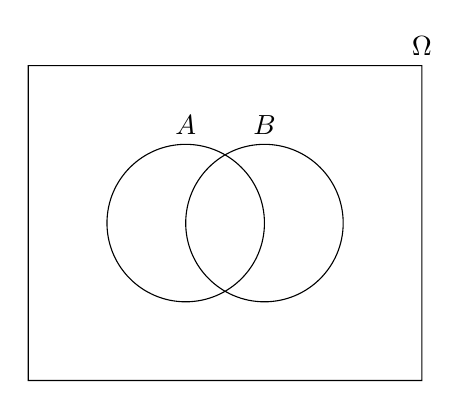
\begin{tikzpicture}[fill=white]
% left hand
\scope
\clip (-2,-2) rectangle (2,2)
      (1,0) circle (1);
\fill[white] (0,0) circle (1);
\endscope
% right hand
\scope
\clip (-2,-2) rectangle (2,2)
      (0,0) circle (1);
\fill[white] (1,0) circle (1);
\endscope
% outline
\draw (0,0) circle (1) (0,1)  node [text=black,above] {$A$}
      (1,0) circle (1) (1,1)  node [text=black,above] {$B$}
      (-2,-2) rectangle (3,2) node [text=black,above] {$\Omega$};
\end{tikzpicture} & &
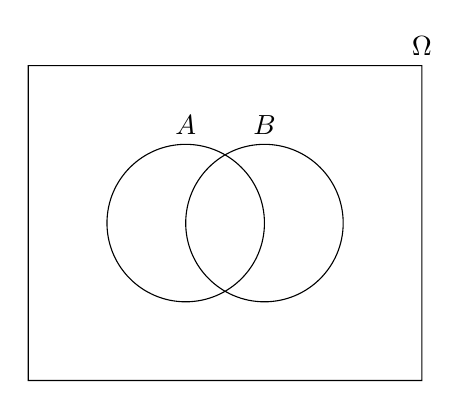
\begin{tikzpicture}[fill=white]
% left hand
\scope
\clip (-2,-2) rectangle (2,2)
      (1,0) circle (1);
\fill[white] (0,0) circle (1);
\endscope
% right hand
\scope
\clip (-2,-2) rectangle (2,2)
      (0,0) circle (1);
\fill[white] (1,0) circle (1);
\endscope
% outline
\draw (0,0) circle (1) (0,1)  node [text=black,above] {$A$}
      (1,0) circle (1) (1,1)  node [text=black,above] {$B$}
      (-2,-2) rectangle (3,2) node [text=black,above] {$\Omega$};
\end{tikzpicture} \\
 &  & \\
  &  & \\
(c) $A \cap B$ & & (d) $A-B$\\
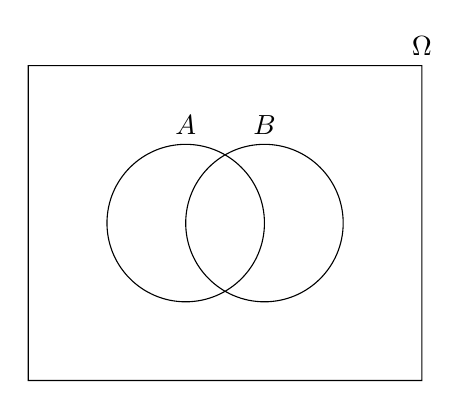
\begin{tikzpicture}[fill=white]
% left hand
\scope
\clip (-2,-2) rectangle (2,2)
      (1,0) circle (1);
\fill[white] (0,0) circle (1);
\endscope
% right hand
\scope
\clip (-2,-2) rectangle (2,2)
      (0,0) circle (1);
\fill[white] (1,0) circle (1);
\endscope
% outline
\draw (0,0) circle (1) (0,1)  node [text=black,above] {$A$}
      (1,0) circle (1) (1,1)  node [text=black,above] {$B$}
      (-2,-2) rectangle (3,2) node [text=black,above] {$\Omega$};
\end{tikzpicture} & &
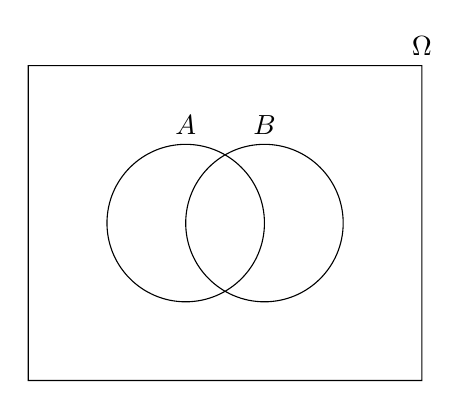
\begin{tikzpicture}[fill=white]
% left hand
\scope
\clip (-2,-2) rectangle (2,2)
      (1,0) circle (1);
\fill[white] (0,0) circle (1);
\endscope
% right hand
\scope
\clip (-2,-2) rectangle (2,2)
      (0,0) circle (1);
\fill[white] (1,0) circle (1);
\endscope
% outline
\draw (0,0) circle (1) (0,1)  node [text=black,above] {$A$}
      (1,0) circle (1) (1,1)  node [text=black,above] {$B$}
      (-2,-2) rectangle (3,2) node [text=black,above] {$\Omega$};
\end{tikzpicture}
\end{tabular}
\ee

%\clearpage

%\pagebegin{Important Venn Diagrams}


%\begin{center}
%\includegraphics[width=3in]{03/03-venn_student.jpg} \ \ \ \ \ 
%\includegraphics[width=3in]{03/03-web_venn.png}
%\end{center}

%\vspace{0.75in}

%\begin{center}
%\includegraphics[width=3in]{03/03-venn_drwho.jpg} \ \ \ \ \ \ 
%\includegraphics[width=2in]{03/03-denzel_venn.png}
%\end{center}


\clearpage
\pagebegin{Probability Rules}

We can generalize the calculations from the previous case study on vitamin A and childhood morbidity to obtain the following results:

\bbox
\begin{theorem}
Let $A$ and $B$ denote two events in sample space $\Omega$, then
\bi
\ii \textbf{\alert{Additive rule}}: $P(A \cup B) = P(A) + P(B) - P(A \cap B)$.
\ii \textbf{\alert{Bayes' Theorem}}: $\dsty P(B | A) = \frac{P(A \cap B)}{P(A)}$
\ii \textbf{\alert{Multiplicative rule}}: $P(A \cap B) = P(A) \cdot P(B | A)$
\ii \textbf{\alert{Complement rule}}: $P(A^C) = 1 - P(A)$
\ei
\end{theorem}
\ebox

\bb[resume] 
\ii When a customer purchases a new car, they are presented with a menu of options such as heated steering wheel, parking assistant, satellite radio, etc. The two most popular options on a certain type of new car are a sunroof (denoted $S$) and heated seats (denoted by $H$). Answer the following questions if we know that 
\[ P(S) = 0.6, \quad P(H) = 0.45,\mbox{ and} \quad P(H | S ) = 0.65 \] \label{q:cars}

\bb
\ii Interpret the practical meaning of $P(H | S ) = 0.65$. \vfill
\ii Compute $P(H^C)$ and interpret the meaning. \vfill
\ii Compute $P(S \cap H)$ and interpret the meaning. \vfill
\ii Compute $P(S | H)$ and interpret the meaning. \vfill
\ee
\ee

\clearpage

\pagebegin{Independent Events}

Often in statistics we want to investigate questions such as:
\bi
\ii Is a newly developed vaccine effective?
\ii Do certain sentencing laws have an effect on crime rates?
\ii Did increasing the minimum wage for fast food workers effect fast food prices?
\ii \textbf{Does the occurrence of one event (getting a sunroof) effect the likelihood that another event (heated seats) occurs?}
\ei

\bb[resume]
\ii In the car option example in question \ref{q:cars}, we know that  $P(S) = 0.6$, $P(H) = 0.45$, and $P(H | S ) = 0.65$. Based on this information, \textbf{if a customer has purchased the sunroof option, are they more, less, or equally likely to get the heated seats option?} Explain how you determined your answer.

\vfill


\ee

\bbox
\begin{definition}\label{def:ind}
Two events $A$ and $B$ are \textbf{\alert{independent}} if the occurrence of one has no effect on the occurrence of the other:

\vspace{0.5in}

%\[ P(B) = P(B | A) \quad \mbox{or} \quad P(A) = P(A | B), \]
\alert{Special case:} If events $A$ and $B$ are independent events then we have $P(A \cap B) = P(A)P(B)$.
\end{definition}
\ebox

\bb[resume]

\ii A person flips a fair coin and stops once they get at least one head and one tail. What is the probability that it takes exactly four flips to get exactly one head and one tail.

\vfill

\ee

\clearpage

%\ii Assume that the overall risk of breast cancer in a 45 year old woman is 1\%. The mammogram test used to screen for
%breast cancer is 90\% \textbf{sensitive}, meaning the test gives a correct positive 90\% of the time. We also know that the mammogram test is 95\% \textbf{specific}, meaning the test gives a correct negative 95\% of the time.\label{medical}
%%Let $D$ denote the event that a 45 year old woman has breast cancer (so $D^C$ is the event she is cancer free). Let $X$ denote the event that the mammogram result is positive for breast cancer (so $X^C$ is the event the screening comes back negative). 
%%\begin{multicols}{2}

%\begin{center}
%\begin{tabular}{c||c|c||c}
%\hline
%\  & $X$, Test Positive & $X^C$, Test negative & Total\\
%\hline
%\hline
%$D$, does have breast cancer &  &  & \\
%\hline
%$D^C$, does NOT have breast cancer &  &  & \\
%\hline
%\hline
%Total &  &  & $100$
%\end{tabular}
%\end{center}

%%\columnbreak
%\bb
%\ii For example, if 100 woman take a mammogram test, fill in the rest of the blanks to complete the \textbf{contingency table} above. \ss
%\ii Are events $D$ and $X$ independent? Show or explain why or why not? \vfill
%%\ee
%%\end{multicols}
%%\bb
%%\addtocounter{enumii}{2}
%\ii What is the probability that a randomly selected 45 year old woman has breast cancer and has a positive test result? \vfill
%\ii What is the probability that a randomly selected 45 year old woman has breast cancer or has a positive test result? \vfill
%\ii You are a doctor who has a 45 year old female patient whose mammogram result is positive. How likely is this patient
%to actually have breast cancer?\vfill
%\ee
%\ee

%\bb[resume]
%\ii According to Lord Mersey's original report to the British Parliament in 1912, there were a total of $2,\!224$ passengers and crew aboard the Titanic when it sank, resulting in the death of $1,\!513$ passengers and crew.  The \textbf{contingency} (or two-way) table shows the passenger breakdown. Let $A_1$, $A_2$, $A_3$ and $A_4$ be the event a randomly selected person onboard the Titanic is first-class, second-class, third-class or crew. Let $S$ be the event the passenger survived.

%\begin{multicols}{2}

%\begin{center}
%\begin{tabular}{c||c|c||c}
%\hline
%\  & Survived & Died & Total\\
%\hline
%\hline
%1st & 203 & 122 & 325\\
%\hline
%2nd & 118 & 167 & 285\\
%\hline
%3rd & 178 & 528 & 706\\
%\hline
%Crew & 212 & 696 & 908\\
%\hline
%\hline
%Total & 711 & 1,\!513 & 2,\!224
%\end{tabular}
%\end{center}

%\columnbreak

%\bb
%%\ii What is the probability that a randomly selected passenger on the Titanic survived?
%\ii Are events $A_2$ and $S$ independent? Show why or why not?
%\ee
%\end{multicols}
%\bb
%\addtocounter{enumii}{1}
%\ii What is the probability that a randomly selected passenger survived and was second-class? \vfill
%\ii What is the probability that a randomly selected passenger survived or was second-class? \vfill
%\ii What is the probability that a randomly selected passenger survived given that we know the passenger was second-class? \vfill
%\ii What is the probability that a randomly selected passenger was second-class class given that we know the passenger survived? \vfill
%\ee
%\ee

%\clearpage

%\pagebegin{Conditional Probabilities}

%\bb[resume]
%\ii Based on your work in \ref{medical}, fill in the blank in definition \ref{def:conditional} below.
%\ee

%\bbox
%\begin{definition}\label{def:conditional}
%If $P(B) >0$, then the \textbf{conditional probability} of $A$ given $B$ is denoted
%\[ P(A \mid B) = \rule{0.2\tw}{0.5pt}.\]
%\end{definition}
%\ebox

%\bb[resume]
%\ii Complete the lemma by filling each blank with one of the following: $P(A \mid B)$, $P(B \mid A)$, $P(A \cap B)$, $P(A)$, or $P(B)$.
%\begin{lemma}\label{lemma:conditional}
%From definition \ref{def:conditional} it follows that
%\bi
%\ii $P(A \cap B) = $ \rule{0.1\tw}{0.5pt} $\cdot P(B) = $ \rule{0.1\tw}{0.5pt} $\cdot P(A)$. \bs
%\ii If $A$ and $B$ are independent events, then $P(A \mid B) = $ \rule{0.1\tw}{0.5pt} .
%\ei
%\end{lemma}
%\ee


\clearpage

\pagebegin{Probability Distributions}

\bbox
\begin{definition}
Two events $A$ and $B$ are \textbf{disjoint} (or \textbf{mutually exclusive}) if they cannot occur at the same time, and therefore $P(A \cap B) = 0$.
\smallskip

\alert{Special case:} If events $A$ and $B$ are disjoint then we have $P(A \cup B) = P(A)+P(B)$.
\end{definition}
\ebox

%\bb[resume]
%\ii Returning to the job applicants example in \ref{applicants}, give an example of:\label{disjoint}
%\bb
%\ii Three different events that are disjoint from one another.\label{aredisjoint} \vfill
%\ii Two different events that are NOT disjoint from one another.\label{notdisjoint} \vfill
%\ee
%\ee


\bb[resume]
%\ii Do the three events you identified in \ref{aredisjoint} form a partition of the sample space $S$ in \ref{applicants}? Show or explain why or why not.
\ii In the options for a new car example in question \ref{q:cars}, are events $H$ and $S$ mutually exclusive? Why or why not? \vfill

\ee

\bbox
\begin{definition}\label{def:prob-dist}
A function $P$ that assigns a real number $P(A)$ to each event $A$ is a \textbf{probability distribution} or a \textbf{probability measure} if it satisfies the following three axioms:
\bb
\ii $P(A) \geq$ \rule{0.1\tw}{0.5pt} for all $A$. \bs
\ii $P(\mbox{full sample space})=P(\Omega) =$ \rule{0.1\tw}{0.5pt} . \bs
\ii If $A$ and $B$ are disjoint, then
\[ P \left( A \cup B \right) = \mbox{\rule{0.25\tw}{0.5pt}}.\]
\ee
\end{definition}
\ebox

%\bb[resume]
%\ii Prove that as a result of definition \ref{def:prob-dist} it follows that $P(A) = 1-P(A^C)$.'\vfill \vspace{1in}

%\ii A fair coin is tossed until we get exactly two heads. What is $\Omega$, the sample space? What is the subset, call it $A$, that corresponds to requiring exactly 4 tosses? What is $A^C$?

%\ee

\clearpage

\pagebegin{OPTIONAL: Counting}


\bb[resume]
\ii 5 people have volunteered to work on a committee. The committee will consist of a total of three people. How many different committees of 3 people can be formed from the 5 volunteers? \vfill
\ee


\bbox
We often need to count the number of ways of choosing $k$ items out of $n$ possible items. You may recall this is often called \textbf{$\mathbf{n}$ choose $\mathbf{k}$} and is denoted as

\[ \left( \begin{array}{c} n \\ k \end{array}\right) = \frac{n!}{k!(n-k)!}.\]
\ebox

\bb[resume]
\ii BONUS: Suppose $n$ people are in a room. What is the probability that there is at least one pair of people that have the same birthday? \textit{Hint: Let $A$ be the event there is no match. Calculate $P(A)$, and then find $P(A^C)$.} %\vfill

\vfill

\ee



%\clearpage

\begin{center}
\includegraphics[width=5in]{03/tyson-tweet.png}
\end{center}
\bs

%\bbox
%\bi 
%\ii A \textbf{statistical experiment or observation} is any random activity that results in a definite outcome.
%\ii The \textbf{sample space} $\Omega$ is the set of all possible outcomes of an experiment.
%\ii An \textbf{outcome, realization or elements}, $\omega$, is a result from an experiment or observation.
%\ii An \textbf{event}, $A$, is a collection of one or more outcomes from an experiment or observation.
%\ei
%\ebox

%\bb
%\ii There are two people in a room. You ask each person what is their birthday (excluding the year).
%\bb
%\ii List several outcomes in the sample space. How many outcomes are in the sample space $\Omega$? \vfill
%\ii Let $M$ denote the event that the two people have the same birthday. How many outcomes are in this event? \vfill
%\ee

%\ii At the end of the semester I randomly select a student in the course and observe their average for the semester.
%\bb
%\ii What is the sample space $\Omega$? \vfill
%\ii What is the event that a student passes the course? \vfill
%\ee

%\ii If possible, give an example of an \textbf{infinite sample space} that is \textbf{discrete}? \vfill

%\ee


\clearpage

\pagebegin{OPTIONAL: Bayes' Theorem}

\bbox
\begin{definition}
A \textbf{partition} of a space $\Omega$ is a collection of disjoint sets such that $\dsty \bigcup_{i=1}^{\infty} A_i = \Omega$.
\end{definition}
\ebox



%%%%%%%%%%%%%%
%% Move elsewhere
%%%%%%%%%%%%%%
\bb[resume]

\ii Fill in the blank to complete theorem \ref{thm:total-prob} below and explain (in words, pictures, or equations) how you determined your answer.

\begin{multicols}{2}

\includegraphics[width=0.4\tw]{03/03-venn-totalprob.jpg}

\columnbreak
\bbox
\begin{theorem}{Law of Total Probability}\label{thm:total-prob}
Let $A_1$, $A_2$, $\ldots , A_k$ be a partition of $\Omega$. Then for any event $B$,
\[ P(B) = \sum_{i=1}^k \rule{0.2\tw}{0.5pt}.\]
\end{theorem}
\ebox

\end{multicols}
\ee

%%%%%%%%%%%%%%
%% Move elsewhere
%%%%%%%%%%%%%%


\clearpage

\bbox
\begin{theorem}{Bayes' Theorem}\label{thm:bayes}
Let $A_1$, $A_2$, $\ldots , A_k$ be a partition of $\Omega$ such that $P(A_i)>0$ for each $i$. If $B$ is any event with $P(B)>0$, then for each $i=1, \ldots k$, we have
Then for any event $B$,
\[ P(A_i \mid B) = \frac{P(A_i \cap B) }{P(B)} = \frac{P(B \mid A_i) P(A_i)}{\sum_{j=1}^k P(B \mid A_j)P(A_j)}.\]
\end{theorem}
\ebox

\bb[resume]
\ii Suppose that 30\% of computers run Mac, 50\% use PC, and 20\% use Linux. A computer virus is
created by hackers, and suppose that  65\% of Mac, 82\% of PC, and 50\% of Linux computers get the virus.
\bb
\ii What is the probability that a randomly selected computer has the virus? \vfill
\ii What is the probability that a randomly selected computer is PC given that the computer is infected by the virus?\vfill \vspace{1in}
\ee
\ee

%\ii Recall the Monty Hall problem. Imagine you are playing the game and initially select door number 1. The game show host than opens one of the other doors (door 2 or door 3) to reveal one of the goats. Let $W$ denote the event the contest wins after making their decision (either \textit{Switch} or \textit{Stay}).
%\bb
%\ii Calculate $P(W \mid \mbox{\textit{Stay}})$. \vfill
%\ii Calculate $P(W \mid \mbox{\textit{Switch}})$. \vfill
%\ii What is the best strategy?  \vfill
%\ii Are $W$ and \textit{Stay} independent events? Mutually exclusive events? \vfill
%\ee
  %Prob Chap 1 Sec 1.1-1.3 Intro to Prob (was 01) and   Sec 1.4-1.5 Condition and Ind (was 02)
%UNIT 1: QUALITATIVE AND GRAPHICAL APPROACHES
% Is first part of original 01.tex
%%%%%%%%%%%%%%%%%%%%%%%%%%%
%%%% Put the following at the top of each .tex file  %
\pagestyle{fancy}
\renewcommand{\theUnit}{2}
\ifthenelse{\isundefined{\UnitPageNumbers}}{}{\setcounter{page}{1}}
\rhead{Carlton and Devore Chapter \theUnit: Discrete Random Variables}
\lhead{Math 3382: Statistical Theory}
%\lhead{\includegraphics[width=1.25cm]{CUDenver-Logo.png}}
\rfoot{\mypage}
\cfoot{\includegraphics[width=2.25cm]{CUDenver-Logo-coverpage.png}}
\lfoot{Adam Spiegler}
\fancypagestyle{firstfooter}{\footskip = 50pt}
\renewcommand{\footrulewidth}{.4pt}
%%%%%%%%%%%%%%%%%%%%%%%%%%%
\vspace*{-20pt} \thispagestyle{firstfooter}

\pagebegin{Introduction to Random Variables}

Suppose a company knows that 1\% of the lithium batteries they manufacture are defective.  The manufacturer sends a shipment of 10 batteries to one of their clients. How likely is it that none of the batteries are defective? How can we connect the data to the concepts of sample spaces and events to answer this question? This link can be made using \textbf{\alert{random variables}}:

\begin{tcolorbox}
\begin{definition}\label{def:rv}
A \textbf{\alert{random variable}} is a mapping
\[ X: \Omega \to \mathbb{R} \]
that assigns a real number $X(\omega)$ to each outcome $\omega \in \Omega$.
\end{definition}
\end{tcolorbox}

For example, the random variable $X$ could map an outcome in which 10 batteries are selected at random to a number corresponding to how many batteries in the sample are not defective, denoted $G$ for good. For instance if $\omega = DDGGGGGGGG$, then $X(DDGGGGGGGG)=8$. We can calculate the probability that $X=10$ (none are defective) using independence of events:
\[ P(X=10) = P(G)P(G) \cdots P(G) = (P(G))^{10} = (0.99)^{10} \approx 0.9044.\]

\bb
\ii A student takes a 3 question quiz. Each of the 3 questions is multiple choice with 4 possible answer choices. Let the random variable $X$ be the number of correct guesses out of the 3 questions.\label{quiz}
\bb
\ii What is the sample space $\Omega$?\label{quizA}
\vspace{0.75in}
\ii Compute $P(X=0)$, how likely is it that the student gets none of the questions correct?
\vspace{0.75in}
\ii Fill in the empty entries in table below

\begin{center}
\begin{tabular}{|c|c|c|c|c|}
\hline
$x$ & \hspace{0.25in} 0  \hspace{0.25in} &  \hspace{0.25in} 1  \hspace{0.25in} &  \hspace{0.25in} 2  \hspace{0.25in} &  \hspace{0.25in} 3  \hspace{0.25in} \\
\hline
 & & & & \\
$P(X=x)$ & & & & \\
 & & & & \\
\hline
\end{tabular}
\end{center}

\ii Compute $P(X \leq 1)$ and interpret the practical meaning of this value.
\ee
\ee

\clearpage

\pagebegin{Distribution Functions}

\begin{tcolorbox}
\begin{definition}\label{def:pmf}
If $X$ is a \textbf{\alert{discrete}} random variable, we define the probability function or \textbf{\alert{probability distribution}} or \textbf{\alert{probability mass function (pmf)}}
for $X$ by
\[ p(x) = P(X=x) .\]
\end{definition}

\vspace{-0.25in}

\begin{definition}\label{def:cdf1}
If $X$ is a random variable, we define the \textbf{\alert{cumulative distribution function (cdf)}} as the function
\[ F(x)=P(X \leq x) = \sum_{k=\mbox{\scriptsize{min value}}}^x p(k) .\]
\end{definition}
\end{tcolorbox}

% Below is a geogebra interactive thing with binomial
% https://www.geogebra.org/m/GyYQWWNX

\bb[resume]
\ii Sketch the pmf and cdf for the random variable $X$ (number of correct guesses on the 3 question quiz) in question \ref{quiz}. Be sure to label the tickmarks on the vertical axes with an appropriate scale.

\begin{center}
\begin{tabular}{ll}
\includegraphics[width=0.3\tw]{04/04-blank-pmf.png} \hspace{1in} &
\includegraphics[width=0.3\tw]{04/04-blank-cdf.png} \\
Sketch the pmf, $p(x)$. & Sketch the cdf, $F(x)$\\
\end{tabular}
\end{center}

\ii Let $X$ is a discrete random variable with pmf and cdf denoted $p(x)$ and $F(x)$, respectively. Determine if each statement is True or False.
\begin{tasks}[counter-format = {(tsk[a])},label-offset = {0.8em},label-format = {\color{black}}](2)
\task $0 \leq p(x) \leq 1$ for all $x$.
\task $0 \leq F(x) \leq 1$ for all $x$. \vspace{0.45in}
\task $\dsty \sum_{\mbox{all $x$}} p(x) = 1$.
\task $\dsty \sum_{\mbox{all $x$}} F(x) = 1$. \vspace{0.45in}
\task $\dsty \lim_{x \to \infty} p(x) = 1$.
\task $\dsty \lim_{x \to \infty} F(x) = 1$. \vspace{0.45in}
\task The pmf must be a nondecreasing function.
\task The cdf must be a nondecreasing function. \vspace{0.45in}
\end{tasks}
\ee

\clearpage

\pagebegin{Expected Value and Variance}

\begin{tcolorbox}
\begin{definition}\label{def:expected}
The average or \textbf{\alert{expected value}} for a discrete random variable $X$ is denote $E(X)$ or $\mu$ and computed using the formula
\[ E(X) = \mu =  \sum_x \left( x \cdot p(x) \right) = \sum_x \left( x \cdot P(X=x) \right). \]
\end{definition}
\vspace{-0.5in}

\begin{definition}\label{def:variance}
The \textbf{\alert{variance}} for a discrete random variable $X$ is one common way to measure how spread out (in relation to the expected value) are the values of $X$. The variance is denoted $\Var(X)$ or $\sigma^2$ and computed using the formula
\[ \Var(X) = \sigma^2 =  \sum_x \left( (x-\mu)^2 \cdot p(x) \right) = \sum_x \left( (x-\mu)^2 \cdot P(X=x) \right). \]
\end{definition}
\vspace{-0.5in}

\begin{definition}\label{def:variance}
The \textbf{\alert{standard deviation}} for a discrete random variable $X$ is the square root of the variance and is denoted by $\sigma$. It more or less measures the average of the distances for each value of $X$ from the mean $\mu$.
\[ \mbox{SD}(X) = \sigma =  \sqrt{\Var(X)}. \]
\end{definition}


\end{tcolorbox}

\bb[resume]
\ii Using properties of the pmf, $p(x)$, show that \label{var-prop}
\begin{tcolorbox}
\[ \Var(X) = E(X^2)  - \mu^2  \]
\end{tcolorbox}

\vspace{0.5in}
\vfill

\ii A charity is running a raffle as afundraiser. They offer one grand prize of \$$500$, two second prizes of \$$100$ each, and ten third prizes of \$$20$ each. They plan to sell $1,\!000$ tickets each at a price of \$$2$. Let $X$ denote the amount of money won by a lottery ticket.\label{lottery}
\bb
\ii Fill in the values of $x$ and $p(x)$ in the table below.\medskip

\begin{center}
\begin{tabular}{|c||c|c|c|c|}
\hline
$x$ &  \hspace{0.5in}  &  \hspace{0.5in}  &  \hspace{0.5in}  &  \hspace{0.5in} \\
\hline
$p(x)$ & & & &  \\
\hline
\end{tabular}
\end{center} \medskip
%\begin{center}
%\begin{tabular}{c|c|c}
%x & \hspace{0.5in} P(x) \hspace{0.5in} & \hspace{1in} $(x-\mu)^2$ \hspace{1in}  \\
%\hline
 % & & \\
 %   & & \\
%\hline
%  & & \\
 %   & & \\
%\hline
%  & & \\
 %   & & \\
%\hline
%  & & \\
 %   & & \\
%\end{tabular}
%\end{center}  \medskip

\ii Calculate $E(X)$ and $\Var(X)$.
\ee
\ee
\vfill
  %Prob Chap 2 Discrete RV (was 03)
%UNIT 1: QUALITATIVE AND GRAPHICAL APPROACHES
% Is first part of original 01.tex
%%%%%%%%%%%%%%%%%%%%%%%%%%%
%%%% Put the following at the top of each .tex file  %
\pagestyle{fancy}
\renewcommand{\theUnit}{2}
\ifthenelse{\isundefined{\UnitPageNumbers}}{}{\setcounter{page}{1}}
\rhead{Carlton and Devore Chapter \theUnit: Discrete Random Variables}
\lhead{Math 3382: Statistical Theory}
%\lhead{\includegraphics[width=1.25cm]{CUDenver-Logo.png}}
\rfoot{\mypage}
\cfoot{\includegraphics[width=2.25cm]{CUDenver-Logo-coverpage.png}}
\lfoot{Adam Spiegler}
\fancypagestyle{firstfooter}{\footskip = 50pt}
\renewcommand{\footrulewidth}{.4pt}
%%%%%%%%%%%%%%%%%%%%%%%%%%%
\vspace*{-20pt} \thispagestyle{firstfooter}

\pagebegin{Discrete Random Variables}

\bb
\ii Suppose a company knows that 1\% of the lithium batteries they manufacture are defective.  The manufacturer sends a shipment of 10 batteries to one of their clients. Let the random variable $X$ denote the number of good (not defective) batteries in the shipment. How likely is it that exactly two of the batteries are defective? \label{q:batteries}

\bb
\ii What is the probability of getting the outcome $GGGGGGGGDD$? Note $G$ and $D$ denote good and defective batteries, respectively. \vfill
\ii How many outcomes are in the event exactly 2 out of 10 batteries are defective? \vfill
\ii Calculate $P(X=8)$. \vfill
\ee

\ii Generalize the result in the previous example. If you repeat $n$ trials which are independent from one another, and each has the same probability of success, $p$, what is the probability of getting exactly $s$ successes out of $n$ trials? \bigskip

$\dsty f(s) = P(X=s) =$   \bigskip

\ii How many good batteries would you expect to receive if you had a shipment of 100 batteries (where it is known that $1$\% of all batteries are defective)? If you received a shipment of 200 batteries? A shipment of 10 batteries? \vfill

\ii Write a general formula for the expected number of successes when $n$ trials are repeated with probability of success $p$ in each trial. \vfill

\ee

\clearpage

\pagebegin{Binomial Distributions}

\begin{tcolorbox}
\bi
\ii A \textbf{\colorb{Bernoulli trial}} is an experiment that has \textbf{\colorb{exactly two possible outcomes}}:
\bi
\ii[$\circ$] The probability that the outcome of a trial is a \colorb{success} ($X=1$ ) is denoted \colorb{$p$}.
\ii[$\circ$] Otherwise, the probability of a \colorr{failure} ($X=0$ ) is \colorr{$q=1-p$}.
\ii[$\circ$] $X$ has a \textbf{\colorb{Bernoulli Distribution}} with probability mass function
\[ f(x) = p^x(1-p)^{1-x} \ \ , \mbox{for } x \in \left\{ 0, 1 \right\}.\]
\ei

\ii Let random variable $X$ be the number of successes out of $n$ trials, where \colorb{each trial is identical and independent}. 
\bi
\ii[$\circ$] $X$ has a \textbf{\colorb{Binomial Distribution}}, written $X \sim \mbox{Binomial}(n,p)$.
\ii[$\circ$] The probability mass function is
\[ f(x) = \left\{ \begin{array}{ll} \left( \begin{array}{c} n\\ x \end{array} \right) p^x(1-p)^{n-x} \ \ & \mbox{for } x =0,1,2, \ldots , n\\
 & \\
0 \ \ & \mbox{otherwise} \end{array} \right. .\]
\ii[$\circ$] The expected value can be calculated with the shortcut \colorb{$E(X) = np$}.
\ii[$\circ$] The variance can be calculated with the shortcut \colorb{$\Var(X) = npq$}.
\ei
\ei
\ebox

\medskip

\begin{tcolorbox}
In R, the we can use the functions:
\bi
\ii \colorb{dbinom($x$, $n$, $p$)} calculates the probability of \colorb{exactly $x$ success} out $n$ trials, \colorb{$P(X=x)$}. 
\ii \colorr{pbinom($x$, $n$, $p$)} calculates the probability of \colorr{at most $x$ success} out $n$ trials, \colorr{$P(X \leq x)$}. 
\ei
\end{tcolorbox}

\bb[resume]
\ii Consider the lithium battery example from question \ref{q:batteries}. Write a command in R that computes the given probability.
\bb
\ii Exactly 7 batteries are good. \vfill
\ii At most 8 batteries are good. \vfill
\ii At most 4 batteries are defective. \vfill
\ee
\ee

\clearpage

\pagebegin{Equally Likely Outcomes}

\bb[resume]
\ii Let $X$ be the value of the result of rolling a fair six-sided die.
\bb
\ii Write out the probability mass function $f(x)$. \vfill
\ii What is the expected value of rolling a fair-six sided die? \vfill
\ee
\ee


\bbox
Let $X$ be a discrete random variable with $k$ different outcomes that each have the same likelihood of occurring.
\bi
\ii $X$ has a \textbf{\colorb{uniform distribution}} on $\left\{ 1, 2, 3, \ldots , k \right\}$
\ii The probability mass function is 
\[ f(x) = \left\{ \begin{array}{ll} \frac{1}{k} \ \ & \mbox{for } x = 1, 2, \ldots,  k\\
0 \ \ & \mbox{otherwise} \end{array} \right. .\]
\ii The expected value is $E(X) = \frac{k+1}{2}$.
\ii The variance is $\Var(X) = \frac{k^2-1}{12}$.
\ei 
\ebox

\bb[resume]
\ii A sports marketer for the Denver Nuggets randomly calls people in the Denver area until she encounters someone who attended a Nuggets' game. What is the probability the market encounters $7$ people who did not attend a game before the first success when it is known that 10\% of the population attended a game last season? \vfill
\ee

\clearpage

\pagebegin{Number of Failures Before First Success}


\bbox
If we repeat a Bernoulli trial that has probability of success $p$ for each trial, we can \colorb{count the number of failures, $X$, that occur before the first success.}
\bi
\ii $X$ has a \textbf{\colorb{Geometric Distribution}}, written $X \sim \mbox{Geom}(p)$.
\ii The probability mass function is $\dsty f(x) = q^xp$ for $x \in \lbrace 0, 1, \ldots \rbrace$.
\ii The expected value is $\mu=E(X) = \frac{q}{p}$.
\ii The variance is $\sigma^2 = \Var(X) = \frac{q}{p^2}$.
\ei

\medskip

In R, the we can use the functions:
\bi
\ii \colorb{dgeom($x$, $p$)} calculates the probability of \colorb{exactly $x$ failures} before first success. 
\ii \colorr{pgeom($x$, $p$)} calculates the probability of \colorr{at most $x$ failures} before first success.
\ii There is no fixed number of trials $n$.
\ei 
\ebox

\pagebegin{Number of Occurrences in a Fixed Time Period}

\bbox
The \textbf{\colorb{Poisson distribution}} applies when the average frequency of occurrences in a given time period is known, and each occurrence is independent the others. Let $X$ denote \colorb{the number of occurrences in the given time period}.
\bi
\ii $X \sim \mbox{Poisson}(\lambda)$, where $\lambda$ denotes the mean number of occurrences in the given time.
\ii The probability mass function is $\dsty f(x) = e^{-\lambda} \frac{\lambda^x}{x!}$ for $x \in \lbrace 0, 1, 2, \ldots \rbrace$.
\ii The expected value is $\mu = E(X) = \lambda$.
\ii The variance is $\sigma^2 = \Var(X) = \lambda$ (same as the expected value).
\ei 

\medskip

In R, the we can use the functions:
\bi
\ii \colorb{dpois($x$, $\lambda$)} calculates the probability of \colorb{exactly $x$ occurrences} in the given time.
\ii \colorr{ppois($x$, $\lambda$)} calculates the probability of \colorr{at most $x$ occurrences} in the given time.
\ei %\bigskip
\ebox

\bb[resume]
\ii If there are twelve cars crossing a bridge per minute on average, find the probability of having seventeen or more cars crossing the bridge in a particular minute.
\ee

\vfill

\clearpage

\pagebegin{Practice}

\bb[resume]
\ii For each situation, identify which distribution best describes the distribution of the random variable. Then use a probability distribution function to calculate the probability.
\bb
\ii A online retailer sells an average of 5 big screen TV's on a given day. What is the probability they sell 9 TV's in a day? \vfill
\ii It is known that 3\% of airbags manufactured by a certain car company are defective. What is the probability that the first defective air bag occurs when the fifth item is inspected? \vfill
\ii Recently, a nurse commented that when a patient calls the medical advice line claiming to have the flu, the chance that he or she truly has the flu (and not just a nasty cold) is only about 4\%. Of the next 25 patients calling in claiming to have the flu, what is the probability that exactly 4 patients will have the flu? \vfill
\ee
\ee
  %Prob Chap 2 Discrete RV (was 03)
%UNIT 1: QUALITATIVE AND GRAPHICAL APPROACHES
% Is first part of original 01.tex
%%%%%%%%%%%%%%%%%%%%%%%%%%%
%%%% Put the following at the top of each .tex file  %
\pagestyle{fancy}
\renewcommand{\theUnit}{3}
\ifthenelse{\isundefined{\UnitPageNumbers}}{}{\setcounter{page}{1}}
\rhead{Carlton and Devore Chapter \theUnit: Continuous Random Variables}
\lhead{Math 3382: Statistical Theory}
%\lhead{\includegraphics[width=1.25cm]{CUDenver-Logo.png}}
\rfoot{\mypage}
\cfoot{\includegraphics[width=2.25cm]{CUDenver-Logo-coverpage.png}}
\lfoot{Adam Spiegler}
\fancypagestyle{firstfooter}{\footskip = 50pt}
\renewcommand{\footrulewidth}{.4pt}
%%%%%%%%%%%%%%%%%%%%%%%%%%%
\vspace*{-20pt} \thispagestyle{firstfooter}

\pagebegin{Introduction to Continuous Random Variables}

A manufacturer of lithium batteries measures the weight of each box they ship out to customers. Let $X$ denote the weight (in pounds) of a randomly selected shipment. It is possible that $X=8$ or $X=9$, but the weight could potentially be any value (greater than 0) such as $8.3671$ pounds if they want to be really precise. Recall the previous definition of a random variable below.

\begin{tcolorbox}
\begin{definition}\label{def:crv}
A \textbf{\colorb{random variable}} is a mapping
\[ X: \Omega \to \mathbb{R} \]
that assigns a real number $X(\omega)$ to each outcome $\omega \in \Omega$.
\end{definition}

\bi
\ii With a discrete random variable, the sample space is mapped to the integers (or a subset of the integers).
\ii With a continuous random variable, the sample space is mapped to an interval of values in $\mathbb{R}$.
\ei

\end{tcolorbox}

\bb
\begin{multicols}{2}

\ii Imagine the GPA distribution for all students at a university follows a \textbf{\colorb{uniform distribution}} with GPA's 
of 0 and 4 being the smallest and largest GPA's possible. \label{gpa-uniform}

\bb
\ii Write a formula for probability density function $f_X(x)$ for the uniform distribution. \vspace{0.5in}
\ii What proportion of students earned a GPA between $3$ and $3.5$?
\ee

\columnbreak

\begin{center}
\includegraphics[width=0.45\tw]{06/06gpa-unif.pdf}
\end{center}

\end{multicols} \vspace{0.5in}

\begin{multicols}{2}
\ii The graph of $f_X(x)$ below shows the probability density function for the GPA's of all students at a university.\label{gpa-v}

\bb
\ii What proportion of students at the university have a GPA between 3 and 4? \vspace{0.5in}
\ii What proportion of students at the university have a GPA between 1 and 3?
\ee

\columnbreak

\includegraphics[width=0.5\tw]{06/06gpa-v.pdf}

\end{multicols} \vspace{0.5in}

\ee

\clearpage

\pagebegin{Probability Distributions}

\begin{tcolorbox}
\begin{multicols}{2}

\begin{definition}\label{def:pdf}
If $X$ is a \textbf{continuous} random variable, the \textbf{\colorb{probability density function (pdf)}}, denoted $f(x)$ satisfies the following properties:
\bi
\ii $f(x) \geq 0$ for all $x$,
\ii $\dsty \int_{-\infty}^{\infty} f(x) = 1$, and 
\ii $\dsty P(a < x < b) = \int_a^b f(x) \, dx$
\ei
\end{definition}

\columnbreak

\includegraphics[width=0.5\tw]{06/06area1.png}
\end{multicols}
\end{tcolorbox}

\bb
\ii The probability of a transistor failing between time $x=a$ and $x=b$ months is given by the probability density function\label{transistor}
\[ f(x) = c \int_a^b e^{-cx} \, dx.\]
\bb
\ii If the probability of failure within the first six months, $0 < x < 6$, is 10\%, set up (but do not solve) an equation to find the value of $c$? \vfill
\ii Set up (but do not evaluate) an integral to represent the probability the transistor fails within the second six months ($6<x<12$)? \vfill
\ii Interpret the meaning of $P(X \leq 9)$ and $P(X < 9)$.\vfill
\ee
 \ee

\clearpage

\begin{tcolorbox}
\begin{definition}\label{def:cdf2}
If $X$ is a \textbf{continuous} random variable, the \textbf{\colorb{cumulative distribution function (cdf)}}, denoted $F(x)$ is
\[ P(X < x) = F(x) = \int_{-\infty}^x f(t) \, dt.\]
\textbf{\colorb{In other words, $F(x)$ is an antiderivative of $f$,} and \colorr{$f(x)$ is the derivative of $F(x)$}.}
\end{definition}
\end{tcolorbox}

\bb[resume]
\begin{multicols}{2}
\ii Match the graphs of the density functions (a), (b), and (c)  with the graphs of the cumulative distribution functions I, II, and III.\label{graph-match}
\columnbreak
\includegraphics[width=0.5\tw]{06/06match.png}
\end{multicols}
\ee

%\clearpage

%\pagebegin{Cumulative Distribution Functions: Section 3.1}

%\bb[resume]
%\ii Decide if the function graphed in is a
%probability density function (pdf) or a cumulative distribution
%function (cdf).  Give reasons.  Find the value of $c$.  Sketch and
%label the other function.  (That is, sketch and label the cdf if the
%problem shows a pdf, and the pdf if the problem shows a cdf.)

%\begin{tasks}[counter-format = {(tsk[a])},label-offset = {0.8em},label-format = {\color{black}\bfseries}](2)
%\task \includegraphics[width=0.4\tw]{06/06graph1.png}
%\task \includegraphics[width=0.4\tw]{06/06graph2.png}
%\end{tasks}
%\ee

\pagebegin{Mean, Variance, and Median}

\begin{tcolorbox}
\bi
\ii The \colorb{mean} of a continuous random variable is\label{def:mean}
\[ E(X) = \mu = \int_{-\infty}^{\infty} x \cdot f(x) \, dx.\]
\ii The \colorb{variance} of a continuous random variable is\label{def:variance}
\[ \Var(X) = E(X-\mu)^2 = E(X^2) - \big( E(X) \big)^2  \ \ \ \mbox{(this can be proven similar as with discrete case)}.\] 
\ii The \colorb{median} is the value $x$ such that $P(X < x) = 0.5$. Thus to find the median we solve the following for $x$:\label{def:median}
\[ F(x) = \int_{-\infty}^x f(t) \, dt = 0.5.\]
\ei
\end{tcolorbox}

\clearpage

\pagebegin{Practice}

\bb[resume]
\ii Consider the random variable with pdf
\[ f(x) = \left\{ \begin{array}{ll} \frac{x}{8}, & \hspace{0.2in} 0 \leq x \leq 4 \\ 0, &  \hspace{0.2in} \mbox{otherwise} \end{array} \right. .\]
\bb
\ii Sketch a graph of the pdf, $f$. \vfill
\ii Give a formula for the cdf, $F$, and sketch its graph. \vspace{1in}
\ii Calculate $P(X < 1)$ and illustrate this value on both of your graphs. \vspace{1in}
\ii Calculate $E(X)$. \vspace{1in}
\ii Give the median value and illustrate this value on both of your graphs. \vfill
\ee
\ee

  %Chapter 3 Continuous RV (was 04)
%UNIT 1: QUALITATIVE AND GRAPHICAL APPROACHES
% Is first part of original 01.tex
%%%%%%%%%%%%%%%%%%%%%%%%%%%
%%%% Put the following at the top of each .tex file  %
\pagestyle{fancy}
\renewcommand{\theUnit}{3}
\ifthenelse{\isundefined{\UnitPageNumbers}}{}{\setcounter{page}{1}}
\rhead{Carlton and Devore Chapter \theUnit: Continuous Random Variables}
\lhead{Math 3382: Statistical Theory}
%\lhead{\includegraphics[width=1.25cm]{CUDenver-Logo.png}}
\rfoot{\mypage}
\cfoot{\includegraphics[width=2.25cm]{CUDenver-Logo-coverpage.png}}
\lfoot{Adam Spiegler}
\fancypagestyle{firstfooter}{\footskip = 50pt}
\renewcommand{\footrulewidth}{.4pt}
%%%%%%%%%%%%%%%%%%%%%%%%%%%
\vspace*{-20pt} \thispagestyle{firstfooter}

\pagebegin{Uniform Distributions}

\begin{tcolorbox}
Recall the \textbf{\colorb{uniform distribution}} of GPA's in problem \ref{gpa-uniform}. More generally, if a continuous random variable is uniformly distributed on the interval $\lbrack a , b \rbrack$, then
\bi
\ii The pdf is $\dsty f(x) = \left\{ \begin{array}{ll} \frac{1}{b-a}, & \hspace{12pt} a \leq x \leq b\\ 0, & \hspace{12pt} \mbox{otherwise} \end{array} \right.$.
\ii The cdf is
\[  F(x) = \left\{ \begin{array}{ll} 0, & \hspace{12pt} x<a \\ \frac{x-a}{b-a}, & \hspace{12pt} a \leq x \leq b \\ 1,  & \hspace{12pt}  x>b \end{array} \right.\]
\ii $E(X) = \frac{a+b}{2}$; $\Var(X) = \frac{(b-a)^2}{12}$; Median $=E(X) = \frac{a+b}{2}$.
\ei
\end{tcolorbox}

\pagebegin{Normal Distributions}

\begin{multicols}{2}
There are many cases where the data tends to be distributed symmetrically around a central value with no bias to the left or
right like this\footnote{Photograph by Peter Morenus in conjunction with Professor Linda Strausberg, of the University of Connecticut}:  %Subjects are University of Connecticut genetics students, females in white tops, males in dark tops}:

\columnbreak

\begin{center} \includegraphics[width=3in]{07/07people.png}\end{center}

\end{multicols}

Normal distributions arise in many settings: Heights of people, size of items produced by machines, and most importantly in statistics data sets resulting from many independent random events. \medskip

\begin{tcolorbox}

The shape of a \textbf{\colorb{normal distribution}} are determined by two parameters:
\bi
\ii The \colorr{mean, $\mu$}, is center of the distribution.
\ii The \colorr{standard deviation, $\sigma$}, tells us how wide the distribution is.
\ii If $X$ is normally distributed with mean $\mu$ and standard deviation $\sigma$, we write \colorr{$\mathbf{X \sim N(\mu, \sigma)}$}.
\ei

\end{tcolorbox}

\begin{tabular}{|c|c|}
\hline
\includegraphics[width=0.35\tw]{07/07normal-width.pdf} & \includegraphics[width=0.35\tw]{07/07normal-center.pdf}\\
\hline
{\scriptsize Increasing the standard deviation makes the curve wider.} &
{\scriptsize Increasing the mean shifts the center of the graph.} \\
\hline
\end{tabular}


\clearpage

\pagebegin{Using the Empirical Rule}

\begin{tcolorbox}
\begin{multicols}{2}
The \textbf{\colorb{empirical rule}} for normal distributions:
\bi
\ii 68\% of all values fall within one standard deviation (both above and below) from the mean, and 
\ii 95\% of all values fall within two standard deviations of the mean.
\ii 99.7\% of all values fall within three standard deviations of the mean.
\ei

\columnbreak

\includegraphics[width=0.45\tw]{07/07empirical.pdf}

\end{multicols}
\end{tcolorbox}

\bb[resume]
\ii ``Last night, Israel became the first country ever to pass legislation banning the use of ‘underweight’ models in local ads and publications. The new law employs an interesting tactic: Models must prove that their Body Mass Index (BMI) is higher than the World Health Organization's indication of malnourishment (a BMI of 18.5) by producing an up-to-date medical report — no older than three months — at all shoots to be used in the Israeli market.'' \footnote{Israel Passes Law Requiring Models to Show Health Records and Meet Weight Standards”, New York Magazine by Charlotte Cowles on April 20, 2012}\label{BMI}

\bi
\ii Let $X$ denote the BMI of adult men in Israel. We know that $X \sim N(26,4)$.
\ii Let $Y$ denote the BMI of adult women in Israel. We know that $Y \sim N(26.5,4.5)$.
\ei

\bb
\ii What proportion of the men in Israel have BMI between 26 and 30? \vfill
\ii What proportion of the women in Israel have BMI between 22 and 35.5? \vfill
\ii How many standard deviations from the mean is a male BMI of 21? \vfill
\ee
\ee

\clearpage

\pagebegin{$Z$-Scores and the Standard Normal Distribution}

\begin{tcolorbox}
\begin{definition}\label{def:zscore}
The number of standard deviations a given data value is from the mean is called the
\textbf{\colorb{z-score}} for the value and is calculated using the formula
\[ z = \frac{x-\mu}{\sigma}.\]
\end{definition}
\end{tcolorbox}

For example, the $z$-score of a male with a BMI 21 is $z=\frac{21-26}{4} = -1.25$.

\begin{center}\includegraphics[width=0.75\tw]{07/07normal-stand.png} \end{center}

When you compute the z-score, you are \textbf{\colorr{“standardizing”}} your data.  You describe values in terms of how many standard deviations from they are from the mean. Comparing areas, we see that \\ $P(X<21) = P(Z<-1.25)$.


\bb[resume]
\ii BMI distribution is approximately normal. In Israel, women have mean BMI of $26.5$ with a standard deviation $4.5$.
What proportion of the women in Israel are legally “underweight” (BMI $< 18.5$)?

\bb
\ii Calculate the $z$-score of a Israeli woman with a BMI of $18.5$. \vfill
\ii Interpret the meaning of the value  in part (a), and give an estimate for the proportion of women in Israel who are legally underweight. \vfill
\ee
\ee

\begin{tcolorbox}
The probability density function for normal distribution (or Gaussian) $X \sim N(\mu,\sigma)$ is given by the formula

\[ f(x) = \frac{1}{\sigma\sqrt{2\pi}} e^{-\frac{1}{2} \left( \frac{x-\mu}{\sigma} \right)^2}\]

To find the probability that a woman has a BMI less than $18.5$, we could try to evaluate

\[ P(\mbox{BMI} < 18.5) = \int_{0}^{18.5} \frac{1}{4.5\sqrt{2\pi}} e^{-\frac{1}{2} \left( \frac{x-26.5}{4.5} \right)^2} \, dx\]

YIKES, good luck with that! So we need to find other methods.
\end{tcolorbox}

\clearpage

\pagebegin{Calculating Areas Under Normal Distributions}


\bb[resume]
\ii What proportion of women in Israel are below the $18.5$ BMI limit?
\ee

\vfill

Using the standard normal distribution table:

\includegraphics[width=0.75\tw]{07/07table.png} \medskip

\begin{tcolorbox}
Using R:
\bi
\ii pnorm($x$, $\mu$, $\sigma$)$=P(X<x)$ gives the area to the left of $x$ under $N(\mu,\sigma)$.
\ii pnorm($x$, $\mu$,  $\sigma$, lower.tail=FALSE)$=P(X>x)$ gives the area to the right of $x$ under $N(\mu,\sigma)$.
\ei \medskip

Or you can find the $z$-score and use the standard normal distribution in R as well:
\bi
\ii pnorm($z$, 0,1)$=P(Z<z)$ gives the area to the left of $x$ under $N(0,1)$.
\ii pnorm($z$, 0,  1, lower.tail=FALSE)$=P(Z>z)$ gives the area to the right of $x$ under $N(0,1)$.
\ei
\end{tcolorbox}

\clearpage

\pagebegin{Practice: IQ Scores}

\bb[resume]
\ii Intelligence quotient (IQ) scores are normally distributed. The mean IQ score is 100 points and the standard deviation is 16 points.

\bb
\ii What proportion of people have an IQ score above 116? \vfill
\ii Marilyn vos Savant has been known to have the highest recorded IQ in the world.  The $z$-score of her test result is $z=5.4$.  What is her IQ score? \vfill
\ii What proportion of people have an IQ score between 75 and 100? \vfill
\ii What is the 90th percentile for IQ? In other words, find the IQ score such that 90\% of the people score less than that score. \vfill
\ee
\ee

\bb[resume]
\ii Let $X$ denote the time (in minutes) spent waiting for the next light-rail to arrive at Union Station. Sketch a possible graph for the probability distribution function of $X$. Explain how you determined the shape of your graph. \vfill
\ee

\clearpage

\pagebegin{Exponential Distribution: Section 3.4}


\begin{tcolorbox}
\bi
\ii Uniform distributions model situations in which each outcome has an equally likely chance to occur.
\ii Most people are average height, but there are approximately an equal number of shorter and taller people. This can be modeled using a normal distribution.
\ii Most of the time, you do not need to wait very long for the next light rail. But sometimes, though rarely,  you do get 
stuck waiting a longer amount of time.
\ii The waiting time for the light rail has properties that can be modeled using an \textbf{\colorb{exponential distribution}}.
\ei

If a continuous random variable $X$ is \textbf{\colorb{exponentially distributed}}, the shape of its pdf depends on one parameter, $\lambda = \frac{1}{\mu}$ where $\mu$ denotes the average value of $X$. We write $X \sim Exp(\lambda)$.

\bi
\ii The pdf is $\dsty f(x) = \lambda e^{-\lambda x}$ for $x >0$ where $\lambda = \frac{1}{\mu}$.
\ii $E(X) = \frac{1}{\lambda}=\mu$ and $\Var(X) = \frac{1}{\lambda^2} = \mu^2$.
\ei
\end{tcolorbox}

\pagebegin{Practice: 911 Call Center}

\bb[resume]
\ii At a 911 call center, calls come in at an average rate of one call every two minutes. Let $X$ denote the time that elapses from one call to the next, and assume $X$ has an exponential distribution.

\bb
\ii Give a formula and sketch the graph of the pdf $f$.  \vfill
\ii Find the probability that after a call is received, it takes more than three minutes for the next call to occur. Illustrate this value on your graph.  \vfill

\clearpage


\ii Find a formula for the cdf, $F$.  \vfill
\ii Find a formula for the inverse of the cdf, $F^{-1}$.  \vfill
\ii Ninety-percent of all calls occur within how many minutes of the previous call? Hint: Use your previous answer.  \vfill
\ii Suppose that two minutes have elapsed since the last call. Find the probability that the next call will occur within the next minute.  \vfill
%\ii Find the probability that less than 20 calls occur within an hour.
\ee
\ee



%During the years 1998 - 2012, a total of 29 earthquakes of magnitude greater than $6.5$ have occurred in Papua New Guinea. Assume that the time spent waiting between earthquakes is exponential.

%\bb
%\ii What is the probability that the next earthquake occurs within the next three months?
%\ii Given that six months has passed without an earthquake in Papua New Guinea, what is the probability that the
%next three months will be free of earthquakes?
%\ii What is the probability of zero earthquakes occurring in 2016?
%\ii What is the probability that at least two earthquakes will occur in 2016?
%\ee
  %Chapter 3 Continuous RV (was 04)
\pagestyle{fancy}
\renewcommand{\theUnit}{4}
\ifthenelse{\isundefined{\UnitPageNumbers}}{}{\setcounter{page}{1}}
\rhead{Carlton and Devore Chapter \theUnit: Joint and Marginal Distributions}
\lhead{Math 3382: Statistical Theory}
%\lhead{\includegraphics[width=1.25cm]{CUDenver-Logo.png}}
\rfoot{\mypage}
\cfoot{\includegraphics[width=2.25cm]{CUDenver-Logo-coverpage.png}}
\lfoot{Adam Spiegler}
\fancypagestyle{firstfooter}{\footskip = 50pt}
\renewcommand{\footrulewidth}{.4pt}
%%%%%%%%%%%%%%%%%%%%%%%%%%%
\vspace*{-20pt} \thispagestyle{firstfooter}


%\begin{tasks}[counter-format = {(tsk[a])},label-offset = {0.8em},label-format = {\color{black}\bfseries}](2)

\pagebegin{Joint and Marginal Probability Distributions}
%From section 4.1 of Prob with Applications to Engineering etc

There are many situations in which we more than one random variable will be of interest.

\bb
\ii A large insurance agency services a number of customers who have purchased both a homeowner’s policy and an automobile policy from the agency. For each type of policy, a deductible amount must be specified. For an automobile policy, the choices are $\$100$ and $\$250$, whereas for a homeowner’s policy, the choices are $\$0$, $\$100$, and $\$200$.\label{insurance}


\begin{multicols}{2}
Suppose an individual with both types of policy is selected at random from the agency’s files. Let $A$ be  the deductible amount on the auto policy and $H$ the deductible amount on the homeowner’s policy. The \alert{joint probability mass  function} $p(a,h)=P(A=a \mbox{ and } H=h)$ is given in the table to the right.

\columnbreak

\begin{center}
\begin{tabular}{|c||c|c|c||c|}
\hline
  & \multicolumn{3}{c||}{$H$} & \\
  \hline
   $p(a,h)$ & $0$ & $100$ & $200$ & Total \\
  \hline 
  \hline
  $a=100$ & $0.20$ & $0.10$ & $0.20$ & \\
\hline
  $a=250$ & $0.05$ & $0.15$ & $0.30$ & \\
\hline
  \hline
  Total  & & & &  \\
\hline
\end{tabular}
\end{center}

\end{multicols}

\bb
\ii Interpret the meaning of the value $p(100,0)=0.2$ in this context. \vfill
\ii Compute $P(A=250)$ and interpret the meaning in this context. \vfill
\ii Compute $P(H=100)$ and interpret the meaning in this context. \vfill
\ee
\ee

\bbox
\bi
\ii The \alert{marginal probability mass function} of $X$ is given by
\[ p_X(x) = P(X=x) = \sum_y p(x,y). \]
\ii The \alert{marginal probability mass function} of $Y$ is given by
\[ p_Y(y) = P(Y=y) = \sum_x p(x,y). \]
\ei
\ebox

\bb[resume]
\ii Using the pmf from the insurance example \ref{insurance}, write a piecewise formula for $p_A(a)$ and $p_H(h)$. \vfill
\ee

\clearpage

\pagebegin{Two Continuous Random Variables}
%From section 4.1 of Prob with Applications to Engineering etc

\bbox
Let $X$ and $Y$ be continuous random variables with \alert{joint probability density function} \newline $f(x,y)$.
\bi
\ii The \alert{marginal probability density function} of $X$ is given by
\[ f_X(x) = \int_{-\infty}^{\infty} f(x,y) \, dy. \]
\ii The \alert{marginal probability density function} of $Y$ is given by
\[ f_Y(y) = \int_{-\infty}^{\infty} f(x,y) \, dx. \]
\ei
\ebox


\bb[resume]
\ii A pharmacy operates both a drive-up facility and a walk-up window. On a randomly selected day, let
$X$ be the proportion of time that the drive-up window is in use,
and let $Y$ be the proportion of time that the walk-up window is in use.
Then the set of possible values for the pair $(X, Y)$ is the rectangle $A= \left\{ (x, y): 0 \leq x \leq 1, 0 \leq y \leq 1 \right\}$ in
$\mathbb{R}^2$. Suppose the joint pdf of $(X,Y)$ is given by\label{pharm}

\[ f(x,y) = \left\{ \begin{array}{ll}
\frac{6}{5}(x+y^2) \ \ \ \ , & 0 \leq x \leq 1, 0 \leq y \leq 1\\
0 , & \mbox{otherwise}
\end{array} \right. \]

\bb
\ii Give a formula for $f_X(x)$ (using integrals). \vfill
\ii Use the formula in the previous part to calculate and interpret $P( 0 \leq X \leq \frac{1}{4})$. \vfill
\ii Give a formula for $f_Y(y)$.  \vfill
\ii Set up (but do not evaluate) a double integral to represent $\dsty P \left( 0 \leq X \leq \frac{1}{4} , \ 0 \leq Y \leq \frac{1}{2} \right)$. \vspace{0.5in}
\ee
\ee

\clearpage

\pagebegin{Marginal PDF's for Continuous Random Variables}

\bbox
Let $X$ and $Y$ be continuous random variables with joint pdf $f(x,y)$.
Then for any two dimensional subset $A \subseteq \mathbb{R}^2$,
\[ P\big( (X,Y) \in A \big) = \int \int_A f(x,y) \, dx dy .\]
In particular if $A$ is a rectangular region  $A= \left\{ (x, y): a \leq x \leq b, c \leq y \leq d \right\}$, then 
\[ P\big( a \leq X \leq b, \ c \leq Y \leq d )= \int_c^d \int_a^b f(x,y) \, dx dy .\]
\ebox

\pagebegin{Independent Random Variables}

\bbox
Two random variables $X$ and $Y$ are said to be \alert{independent} if for every part of $x$ and $y$ values,
\[ \alert{f(x,y) = f_X(x) \cdot f_Y(y)}  \ \ \mbox{when $X$ and $Y$ are continuous, or}\]
\[ \alert{p(x,y) = p_X(x) \cdot p_Y(y)}  \ \ \mbox{when $X$ and $Y$ are discrete.}\]
Notice this definition applies when $A$ and $B$ are independent events, then $P(A \cap B) = P(A)P(B)$. 
\ebox

\bb[resume]
\ii In the insurance example \ref{insurance}, are random variables $X$ and $Y$ independent? Explain how you determined your answer, and then interpret the practical significance of your answer.

\vfill

\ii In the pharmacy example \ref{pharm}, are random variables $X$ and $Y$ independent? Explain how you determined your answer, and then interpret the practical significance of your answer.

\ee

\vfill

\clearpage

\pagebegin{Expected Values: Section 4.2}
%Prob with Applications section 4.2

\bbox
%We have previous seen that if $X$ is a random variable with pdf $f_X(x)$, and if we define $Y=g(X)$, then
%\[ E(Y) = E(g(X)) = \int_{-\infty}^{\infty} g(x) \cdot f_X(x) \ dx .\]
 %A similar result holds for a function of two (or more) variables. \medskip

Let $X$ and $Y$ be two random variables with joint pdf $f(x,y)$. If $Z=h(X,Y)$, then
\[ E(Z) = E(h(X,Y)) = \left\{ \begin{array}{ll}
\dsty \int_{-\infty}^{\infty} \int_{-\infty}^{\infty} h(x,y)\cdot f(x,y) \, dx dy , \ \ \ \ \ \ & \mbox{if $X$ and $Y$ are continuous} \\
 & \\
\dsty \sum_y \sum_x h(x,y)\cdot f(x,y) , &  \mbox{if $X$ and $Y$ are discrete} \end{array} \right. .\]
This is often referred to as the \alert{\textit{Law of the Unconscious Statistician}} since we do not need to know $f_Z(z)$
in order to compute $E(Z)$.
\ebox

\bb[resume]
\ii Let $X$ and $Y$ be the values ($1, 2, \ldots ,6$) rolled by each of two die. Assume that $X$ and $Y$ are independent,
and define the random variable $Z=h(x,y)=xy$ which is the product of the two rolls. Calculate $E(Z)$,
the expected value of $Z$, the product of the two rolls.\label{pair-die}
\ee

\vfill

\clearpage

\pagebegin{Expected Value and Variance of Linear Combinations and Products}

\bbox
Let $X$ and $Y$ be two random variables and consider a linear combination $aX+bY$ for $a$ and $b$ two constants.
\bi
\ii Expected value: \alert{$E(aX+bY)=aE(X)+bE(Y)$}
\ii This propery is true regardless of whether $X$ and $Y$ are independent or dependent.
\ei
\ebox

\bb[resume]
\ii Prove that expected value and property above. \vfill
\ee



\bbox
\textbf{A special case for products:} Let $X$ and $Y$ be two \alert{independent} random variables. Then additionally we have the following properties.
\bi
\ii Expected value: \alert{$E(XY) = E(X) \cdot E(Y)$}.
\ii Variance: \alert{$\Var(aX+bY)=a^2\Var(X)+b^2\Var(Y)$}
\ii Variance: \alert{$\Var(XY) = E(X^2Y^2) - \big( E(X)E(Y) \big)^2$}.
\ii \colorr{In general these properties do NOT hold if $X$ and $Y$ are dependent.}
\ei
\ebox



%\bb[resume]
%\ii Suppose that the lifetimes of two components are independent of each other and that the first lifetime, $X$, has an exponential distribution with average lifetime of 1000 hours. The second component, $Y$, has an exponential distribution with parameter $\lambda_2 = 1200$ hours. Then the joint pdf is

%\[ f(x,y) = \left\{ \begin{array}{ll}
%f_{X}(x)f_Y(y) = \frac{1}{1,\!200,\!000}e^{-\frac{x}{1000}-\frac{y}{1200}} \ \ \ , & x>0 , \ y>0 \\
%0 & \mbox{otherwise} \end{array} \right. . \]

%\bb
%\ii Set an integral that represents the probability that the sum of their lifetimes is at most 3000 hours.
%\ii Evaluate the integral in the previous part. %0.7564
%\ee
%\ee
  %Joint and Marginal: Stat with App 4.1 (was 05)
\pagestyle{fancy}
\renewcommand{\theUnit}{4}
\ifthenelse{\isundefined{\UnitPageNumbers}}{}{\setcounter{page}{1}}
\rhead{Chapter \theUnit: Sampling Distributions}
\lhead{Math 3382: Statistical Theory}
%\lhead{\includegraphics[width=1.25cm]{CUDenver-Logo.png}}
\rfoot{\mypage}
\cfoot{\includegraphics[width=2.25cm]{CUDenver-Logo-coverpage.png}}
\lfoot{Adam Spiegler}
\fancypagestyle{firstfooter}{\footskip = 50pt}
\renewcommand{\footrulewidth}{.4pt}
%%%%%%%%%%%%%%%%%%%%%%%%%%%
\vspace*{-20pt} \thispagestyle{firstfooter}


%\begin{tasks}[counter-format = {(tsk[a])},label-offset = {0.8em},label-format = {\color{black}\bfseries}](2)
\pagebegin{Sampling Distributions}

\bbox
\textbf{\colorb{Statistical inference}} is the process of drawing conclusions about the entire population based on information in a sample.
\bigskip

A \textbf{\colorb{sampling distribution}} is the distribution of sample statistics (such as a mean, proportion, median, maximum, etc.) computed for different samples of the same size from the same population. A sampling distribution shows us how the sample statistic varies from sample to sample.
\ebox

\pagebegin{Sampling from Populations with Different Shapes}

For questions 1-3 below, \textbf{\alert{open the RMarkdown file 09\_Sampling\_Dist.Rmd}} and answer the questions in the RMarkdown file by running R code in that file. Then summarize your answers for each question below.

\bb
\ii Let $X$ denote the distribution of BMI of all adult men. We can approximate this distribution by $X \sim N(26, 4)$. \label{q:bmi}
\[ \bar{x} = \frac{x_1 + x_2 + x_3+x_4}{4}. \]


\begin{center}
\begin{tabular}{|l|c|c|c|c|}
\hline
 \ \ & Population & $n=4$ & $n=9$ & $n=16$ \\
\hline
Shape & Normal & \ \ \ \ \ \ \ \ \ \ \ \ \ \ \ \ \ \ \ \ & \ \ \ \ \ \ \ \ \ \ \ \ \ \ \ \ \ \ \ \ & \ \ \ \ \ \ \ \ \ \ \ \ \ \ \ \ \ \ \ \ \\
\hline
Mean & 26 & & & \\
\hline  
Standard Deviation & 4 & & & \\
\hline  
\end{tabular}
\end{center}

\ii  Let $X$ denote the distribution of the time (in minutes) between successive eruptions (called the wait time) of a certain geyser that is modeled by $X \sim \mbox{Exp} \big( \frac{1}{40} \big)$. \label{q:geyser} %https://www.statology.org/exponential-distribution-real-life-examples/

\begin{center}
\begin{tabular}{|l|c|c|c|c|}
\hline
 \ \ & Population & $n=4$ & $n=9$ & $n=16$ \\
\hline
Shape & Skewed \_\_\_\_\_\_\_\_  & \ \ \ \ \ \ \ \ \ \ \ \ \ \ \ \ \ \ \ \ & \ \ \ \ \ \ \ \ \ \ \ \ \ \ \ \ \ \ \ \ & \ \ \ \ \ \ \ \ \ \ \ \ \ \ \ \ \ \ \ \ \\
\hline
Mean & 40 & & & \\
\hline  
Standard Deviation & $\sqrt{40}$ & & & \\
\hline  
\end{tabular}
\end{center}

\ii The dataset  \colorg{quakes}  in R has the locations of 1000 seismic events that occurred near Fiji since 1964 with body wave magnitude (mb)  $> 4.0$. Assume this data represents the population of all such earthquakes near Fiji since 1964. Let $X$ denote the distribution of the depths (in km) where all such earthquakes occurred. Note this data is approximately \alert{bimodal}. \label{q:quake}

\begin{center}
\begin{tabular}{|l|c|c|c|c|}
\hline
 \ \ & Population & $n=4$ & $n=9$ & $n=16$ \\
\hline
Shape & Bimodal & \ \ \ \ \ \ \ \ \ \ \ \ \ \ \ \ \ \ \ \ & \ \ \ \ \ \ \ \ \ \ \ \ \ \ \ \ \ \ \ \ & \ \ \ \ \ \ \ \ \ \ \ \ \ \ \ \ \ \ \ \ \\
\hline
Mean &  & & & \\
\hline  
Standard Deviation &  & & & \\
\hline  
\end{tabular}
\end{center}

\ee


\clearpage

\pagebegin{Notation}

\bbox
\bi
\ii When describing the \alert{mean} of a distribution we use the notation:
\bi
\ii[$\circ$] Population mean: \alert{$\mu_X$}
\ii[$\circ$] Sample mean:  \alert{$\bar{x}$}
\ii[$\circ$] Center of the Sampling distribution for a mean:  \alert{$\mu_{\overline{X}}$}
\ei
\ii When describing the \alert{standard deviation} of a distribution we use the notation:
\bi
\ii[$\circ$] Population standard deviation:  \alert{$\sigma_X$}
\ii[$\circ$] Sample standard deviation:  \alert{$s_X$}
\ii[$\circ$] Spread of the sampling distribution is called the \alert{Standard Error}.
\bi
\ii[$\diamond$] The standard error measures the variability in sample statistics due to randomness.
\ii[$\diamond$] We use the notation \alert{$\mbox{SE}(\overline{X}) = \sigma_{\overline{X}}$}.
\ei
\ei
\ei
\ebox

\bb[resume]
\ii In each of the three sampling distributions we examined, lets summarize what seems to be happening as the size of the samples, $n$, is increased.

\bb
\ii Does the shape of the sampling distribution stay the same as the population or does it change as $n$ increases? \vfill

\ii Does the center of the sampling distribution, $\mu_{\overline{X}}$, stay the same or change as $n$ increases? How does the value of $\mu_{\overline{X}}$ compare to the population mean $\mu_X$? \vfill

\ii Does the standard error of the sampling distribution, $\mbox{SE}(\overline{X})$, stay the same or change as $n$ increases?  \vfill

\ee
\ee

\clearpage

\pagebegin{Central Limit Theorem for Means}

\bbox
Let $X_1, X_2, \ldots , X_n$ be independent, identically distributed (iid) random variables from a population with mean and
standard deviation $\mu$ and $\sigma$, then as long as $n$ is large enough \colorb{($\mathbf{n \geq 30}$)}, the sampling distribution for the mean, $\bar{X}$ will:
\bi
\ii Be (approximately) normally distribution.
\ii Have mean equal to the mean of the population, $\mu$.
\ii Have standard error $\mbox{SE}(\bar{X}) = \frac{\sigma}{\sqrt{n}}$.
\ei

We summarize the results more concisely below:

\alert{ \[ \overline{X} \sim N \left( \mu_{\overline{X}} , \sigma_{\overline{X}} \right) = N \left( \mu  , \frac{\sigma}{\sqrt{n}} \right) \] }

\ebox

\bb[resume]
\ii Recall the distribution of adult male BMI,  $X \sim N(26,4)$, from question \ref{q:bmi} and answer the questions below.

\bb
\ii What is the probability of randomly select one adult man that has a BMI greater than 28? \vfill

\ii If you construct a sampling distribution for the mean BMI of adult males using random samples each size $n=50$, approximate the shape, center, and standard error of the sampling distribution. \vfill

\ii If you construct a sampling distribution for the mean wait time between geyser eruptions using random samples each size $n=100$, approximate the shape, center, and standard error of the sampling distribution. \vfill

\ii What is the probability of picking a random sample of $n=100$ adult men that has a sample mean BMI greater than 28? \vfill
\ee
\ee

\clearpage

\pagebegin{Independent and Identically Distributed Random Variables}

\bbox
The random variables $X_1, X_2, \ldots , X_n$ are said to be \alert{independent and identically distributed (iid)} if
\bi
\ii The $X_i$'s are independent random variables (the value of $X_i$ does not effect the value of $X_j$ for $i \ne j$).
\ii Every $X_i$ has the same probability distribution.
\ii Such a collection of random variables is called a \alert{simple random sample} of size $n$.
\ei
For example:
\bi
\ii Measure the BMI of $n$ randomly selected adult men.
\ii Measure the weight time of $n$ randomly selected eruptions of a geyser.
\ii Measure the depth of $n$ randomly selected $n$ earthquakes that occurred near Fiji since 1964.
\ei
\ebox

  %Chapt 4 Sampling Dist and CLT for Means (was 07)
\pagestyle{fancy}
\renewcommand{\theUnit}{4}
\ifthenelse{\isundefined{\UnitPageNumbers}}{}{\setcounter{page}{1}}
\rhead{Chapter \theUnit: Sampling Distributions}
\lhead{Math 3382: Statistical Theory}
%\lhead{\includegraphics[width=1.25cm]{CUDenver-Logo.png}}
\rfoot{\mypage}
\cfoot{\includegraphics[width=2.25cm]{CUDenver-Logo-coverpage.png}}
\lfoot{Adam Spiegler}
\fancypagestyle{firstfooter}{\footskip = 50pt}
\renewcommand{\footrulewidth}{.4pt}
%%%%%%%%%%%%%%%%%%%%%%%%%%%
\vspace*{-20pt} \thispagestyle{firstfooter}


%\begin{tasks}[counter-format = {(tsk[a])},label-offset = {0.8em},label-format = {\color{black}\bfseries}](2)

\pagebegin{Sampling from a Binomial Distribution}

Very often we encounter statistical questions that ask us to approximate or compare \alert{proportions}. For example
\bi
\ii ``What proportion of voters support a new law?''
\ii ``What proportion of the population follow public health recommendations?''
\ii ``For a certain model smartphone, what proportion of all smartphones produced are defective?''
\ei

\bbox
\bi
\ii In these cases, we have a certain population in mind. A sample size $n$ is randomly selected. 
\bi
\ii[$\circ$] Each selection is considered a trial. We have $n$ trials.
\ii[$\circ$] Since we pick from the same population, the probability of a success in each trial is $p$.
\ii[$\circ$] We count $X$, the number of ``successes'' out of $n$ independent and identical trials.
\ii[$\circ$] Note that we have $X \sim \mbox{Binom}(n,p)$.
\ii[$\circ$] Then we can calculate the sample proportion:
\[ \hat{p} = \frac{\mbox{Number of successes}}{\mbox{Size of sample}} = \frac{X}{n}.\]
\ei
\ii If we repeat this process over and over again (say 1000 times), then we can look at the \alert{Distribution of Sample Proportions} that we denote \alert{$\widehat{P}$}.
\ei
\ebox


\bb
\ii Let $p$ denote the proportion of all packages mailed by the United States Postal Service (USPS) that contain illegal contents. We randomly select a sample of $n$ packages, count the number of illegal packages $x$, and then compute the proportion of packages in the sample that have illegal contents $\hat{p} =\frac{x}{n} $. We repeat this over and over again and construct the distribution of sample proportions, $\widehat{P}$.

\bb
\ii Let $X$ denote the number of successes (illegal packages) out of a random sample of $n$ USPS packages. What are the mean and standard deviation of $X$. Your answers will depend on $n$ and $p$. \vfill

\ii Let $\widehat{P} = \frac{X}{n}$ denote the distribution of sample proportions. Using formulas from part (a) and properties expected value and variance, give formulas for $E( \widehat{P} )$ and $\Var( \widehat{P} )$. \vfill
\ee
\ee

\clearpage

\pagebegin{Central Limit Theorem for Proportions}

\bbox
Let $X \sim \mbox{Binom}(n,p)$ be a binomial random variable, and let $\widehat{P} = \frac{X}{n}$ denote the distribution of sample proportions. Then if the sample is large enough (\colorb{both $\mathbf{np \geq 10}$ and $\mathbf{n(1-p) \geq 10}$}) , the sampling distribution for $\widehat{P}$ will:
\bi
\ii Be (approximately) normally distribution.
\ii Have mean equal to the population proportion, $p$.
\ii Have standard error $\mbox{SE}(\widehat{P}) = \sqrt{\frac{p(1-p)}{n}}$.
\ei

We summarize the results more concisely below:

\alert{ \[ \widehat{P} \sim N \left( \mu_{\widehat{P}} , \sigma_{\widehat{P}} \right) = N \left( p  , \sqrt{\frac{p(1-p)}{n}} \right) \] }
\ebox


\pagebegin{Practice with Central Limit Theorem for Proportions}


\bb[resume]
\ii Census Bureau data for 2017 shows nearly half (48 percent) of residents in United State's five largest cities now speak a language other than English at home\footnote{https://cis.org/Report/Almost-Half-Speak-Foreign-Language-Americas-Largest-Cities}. If a sample of 150 people are selected at random from the five largest cities in the US, what is the probability that at most 40\% speak a language other than English at home? \label{q:language}
\bb
\ii Is $n$ large enough to use the CLT? Explain why or why not? \vfill
\ii Using the CLT for a proportion, find the z-score of the proportions $0.44$ and $0.48$. \vfill
\ii What is the probability that between 44\%  and 48\%(out of the random sample of 150 people) speak a language other than English at home? \label{q:language-no}\vfill
\ee
\ee

\clearpage

\pagebegin{Continuity Correction for Discrete Random Variables}

\bbox
A binomial random variable is a discrete random variable, but a normal distribution approximation is continuous density function.
When using a normal distribution to approximate the sampling distribution for a discrete random variable $X$, we can improve the estimate by using a \textbf{\colorb{continuity correction}} as follows. If we want to calculate $P( a \leq X \leq b)$ where $a<b$ are integers, then we use
the following correction:
\[ P( a \leq X \leq b) \approx P(a-0.5 < X < b+0.5) =  P \left( \frac{(a-0.5)}{n} < \widehat{P} < \frac{(b+0.5)}{n} \right).\]
\ebox

\bb[resume]
\ii In question \ref{q:language-no} we calculated $P\left( 0.44  \leq \widehat{P} \leq 0.48 \right)$ using a normal distribution (by way of the CLT). We could equivalently rewrite this probability in terms of the discrete random variable $X \sim \mbox{Binom}(150,0.48)$ as $P( 66 \leq X \leq 72$).
\bb
\ii Using a binomial distribution, calculate the exact value of $P( 66 \leq X \leq 72$). \label{q:language-exact}. \vfill

\ii Calculate the $z$-score using a corrected lower limit, $\hat{p}_1^* = \frac{66-0.5}{150} = 0.4367$.  \vfill

\ii Calculate the $z$-score using a corrected upper limit, $\hat{p}_2^* = \frac{72+0.5}{150} = 0.4833$.  \vfill

\ii Using the z-scores from parts (b) and (c) obtained by applying a continuity correction, approximate the probability that between 44\% and 48\%(out of the random sample of 150 people) speak a language other than English at home? \label{q:language-yes}  \vfill

\ii Compare approximations from questions \ref{q:language-no} and \ref{q:language-yes} with the exact calculation in question \ref{q:language-exact}. Comment on whether or not the continuity correction improved the approximation or not.  \vfill
\ee
\ee

\clearpage

\pagebegin{Sampling Distributions for Other Statistics}

\bb[resume]
\ii Frequently we are interested in the minimum, denoted $X_{\rm{min}}$, or maximum, denoted $X_{\rm{max}}$ of a set.  Let’s derive the cdf for the maximum of a random sample, $X_1,X_2, \ldots, X_n$ each independently picked from a distribution with  corresponding cdf $F(x)$. \medskip

$\dsty F_{X_{\rm{max}}} (a) = P(X_1 \leq a, X_2 \leq a, \ldots, X_n \leq a) = $
\vfill

\ii Using the result from the previous problem, find $\dsty f_{X_{\rm{max}}} (a)$, the pdf for the maximum of a random sample. \vspace{1in}

\ii Let $X \sim \mbox{Unif}(0,1)$.
\bb
\ii What are the cdf and pdf, $F(x)$ and $f(x)$ respectively, of $X$? \vspace{1in}
\ii If we pick a random sample of size $n=10$, how likely is it that $X_{\rm{max}}$ is greater than or equal to $0.9$? \vspace{2in}
\ee
\ee


  %Chap4 CLT for Props(was 11)
\pagestyle{fancy}
\renewcommand{\theUnit}{5}
\ifthenelse{\isundefined{\UnitPageNumbers}}{}{\setcounter{page}{1}}
\rhead{Chapter \theUnit: Bootstrap Distributions}
\lhead{Math 3382: Statistical Theory}
%\lhead{\includegraphics[width=1.25cm]{CUDenver-Logo.png}}
\rfoot{\mypage}
\cfoot{\includegraphics[width=2.25cm]{CUDenver-Logo-coverpage.png}}
\lfoot{Adam Spiegler}
\fancypagestyle{firstfooter}{\footskip = 50pt}
\renewcommand{\footrulewidth}{.4pt}
%%%%%%%%%%%%%%%%%%%%%%%%%%%
\vspace*{-20pt} \thispagestyle{firstfooter}


%\begin{tasks}[counter-format = {(tsk[a])},label-offset = {0.8em},label-format = {\color{black}\bfseries}](2)

\pagebegin{Chapter 5: Bootstrap Distributions}

A common feature of previous examples is that the distribution for the population(s) was known.
\bi
\ii For example if a coin is fair, then we know the population is binomial with $p=0.5$, and we can answer questions about the probability of certain events occurring.
\ii If we have population $X \sim \mbox{Exp} ( \lambda )$, then we can use CLT to calculate $P( \overline{X} < 10 )$.
\ei

\bbox
What if the population is unknown? When we use data from a sample to describe some characteristic of the population, we are doing statistics!
\bi
\ii A \textbf{\colorb{parameter}} is a characteristic of a population (which may be a probability distribution).
\ii A \textbf{\colorb{statistic}} is a characteristic of a sample.
\ii A parameter is a typically a number (mean, proportion, ratio of two means) that is unknown.
\ii Recall we use different notation for parameters and statistics.
\ii Statistic(s) from a sample can be used to estimate unknown population parameter(s).
\ei
\ebox


\bb
\ii  Imagine you would like to answer the following question?

\begin{center}\textbf{``What is the average weight of all babies that were born this past year?''}\end{center}

How could you go about answering this question?


\ee

\clearpage

\pagebegin{Estimating the Weight of All Newborns}


The dataset \textit{\textbf{\colorg{NCBirths2004}}} from the textbook contains data from a sample of 1009 babies born in North Carolina in 2004 and contains variables \colorr{Age} (mother's age), \colorr{Tobacco} (mother used tobacco?), \colorr{Gender} (gender assigned at birth to baby), \colorr{Weight}, \colorr{Gestation} (gestation period in weeks when born).

\bi
\ii For the purposes of this thought experiment, we will imagine the 1009 observations in \textit{\textbf{\colorg{NCBirths2004}}} is the population.
\ei

\bb[resume]
\ii Open R Studio and from the Console at the bottom enter the commands:\label{q:newborn}
\begin{lstlisting}
library(resampledata) 
my.samp <- sample(NCBirths2004$Weight, 10, replace = FALSE) 
print(my.samp)
\end{lstlisting}

\bb
\ii Write down or take a picture of your data in \textit{\textbf{\colorg{my.samp}}}. \vspace{1in}

\ii Using your random sample \textit{\textbf{\colorg{my.samp}}}, what would be your best estimate for the average weight of all newborns in the population? \vspace{1in}

\ii Do you think your classmates will have the same estimate? How can we account for this variability in our estimate?  \vspace{1in}

\ee

\ee

\bigskip


\bbox
A \textbf{\colorb{statistical question}} is one that can be answered by collecting data and where there will be variability in that data.
\ebox


\clearpage

\pagebegin{Accounting for the Uncertainty of our Estimate}

%\textbf{\colorb{In many situations, we only have one sample, and no claim about the population. How can we construct a sampling distribution in such scenarios?}}

If we had a \textbf{\colorb{sampling distribution}}, we could use the standard error to measure the variability of sample statistics. \textbf{\colorr{But in practice, we only have one sample, and know very little about the population.}}

\bbox
\textbf{\colorb{Bootstrapping}} is a process that uses data from a sample to construct a new distribution called a \textbf{\colorb{bootstrap distribution}} that approximates the distribution for some sample statistic (such as a mean, proportion, variance, and others). %We can use bootstrapping even when the Central Limit Theorem does not apply.
\ms

Given an original sample of size $n$ from a population:
\bi
\ii Draw a resample of size $n$ (same size as original sample) with replacement from the sample. Compute the relevant statistic.
\ii Repeat this many times (say $10,\!000$ times).
\ii Construct the \textbf{\colorb{bootstrap distribution}} of the statistic. Inspect the center, spread and shape.
\ei
\ebox


\bb[resume]
\ii Consider a random sample of 4 baby weights: 3800, 3065, 2950, and 4100. Which of the following could be a possible bootstrap resample? Explain why or why not.
\bb
\ii 3800, 3065, 4100 \vfill
\ii 3800, 3800, 3800, 3800 \vfill
\ii 3800, 3065, 2950, 4100 \vfill
\ii 3800, 3065, 2950, 4100, 4100 \vfill
\ii 3800, 3065, 2950, 3450 \vfill
\ee

\ii How many possible bootstrap resamples can be constructed from an original sample that has $n$ values? \vfill
\ee


\clearpage

\pagebegin{Creating a Bootstrap Distribution}

Let's return to our question: \textbf{\colorg{``What is the average weight of all babies that were born in North Carolina in 2004?''}}

\bi
\ii For us, the population is the 1009 newborns in \textit{\textbf{\colorg{NCBirths2004}}} (but population data is unknown).
\ii From one random sample of 10 newborns picked from the population,  we can create a bootstrap distribution for the sample mean.
\ei

\begin{multicols}{2}
library(resampledata) \\
\\
$N \ <- \ 10^5$ \# number of bootstrap resamples\\
boot.dist $<-$numeric(N) \# array to save stats\\
\\
%\# \textbf{for each bootstrap resample, pick 1009 numbers}\\
%\# \textbf{between 1 and 1009 (with replacement)}\\
%\# \textbf{pick those values in original sample}
%\# \textbf{and compute sample mean}\\
for (i in 1:N)\\
$\left\{ \right.$\\
\indent \ \ \ \  x $<-$ sample(my.samp, 10, replace = TRUE)\\
\indent \ \ \ \ boot.dist[i] $<-$ mean(x) \\
$\left. \right\}$\\
\\
%\# \textbf{Create a histogram of bootstrap sample means}\\
hist(boot.dist,  xlab = "xbar", \\
\indent  \ \ \ \ \ \ \ main = "Bootstrap Distribution")\\
\\
mean(boot.dist)\\ % \#Calculate center of bootstrap dist \\
sd(boot.dist)\\ %\#Calculate center of bootstrap dist \\

\columnbreak

\begin{center}
\includegraphics[width=0.5\tw]{11/fig-ncbirths2.png}
\end{center}

\vspace{-0.25in}

\textbf{\colorb{Bootstrap Center}}  $= 3322.2$g \\
\textbf{Bootstrap Standard Error}   $= 151.98$g\\
\\
\\ 
\textbf{Bias} $=$ \textbf{\colorb{Bootstrap Center}} $-$ \textbf{\colorr{Sample Mean}}\\
\textbf{Bias} $= 3322.2--3322.5=-0.3$g \\
\\
\\
\textbf{Actual Population Mean} $= 3448.26$g\\
\textbf{CLT SE} $= \frac{\mbox{sd(NCBirths2004\$Weight)}}{\sqrt{10}}= 154.2357$g\\
\end{multicols}

%\[ \mbox{index} = \left( \begin{array}{c} 463 \\ 346 \\ 2 \\ \vdots \\ 5 \\ 1004 \end{array} \right) 

\pagebreak

\pagebegin{Comparing CLT with Bootstrapping}

Consider the theoretical population $X \sim N(23,7)$. Below we compare the sampling distribution for the mean obtained using the central limit theorem on the top row with one random sample and a corresponding bootstrap distribution for the sample mean on the bottom row\footnote{See file Chap5-Compare.R for code that created the figure}..

\begin{center}
\includegraphics[width=0.75\tw]{11/fig-compare2.png}
\end{center}

\begin{center}
\begin{tabular}{lll}
\hline
 & Mean \ \ \ \ \ \ \ \ \ \ & Standard deviation \\
 \hline
Population & 23 & 7 \\
Theoretical Sampling Dist for $\bar{X}$ \ \ \ \ \ \ \ \ \ \ & 23 & $0.99$ \\
Sample ($n=50$) & $23.14$ & $6.69$ \\
Bootstrap distribution & $24.15$ & $0.92$\\
\hline
\end{tabular}
\end{center}


\bb[resume]
\ii Compare the population and sample distributions. What is similar about the two distributions? What are the differences? \vfill

\ii Compare the sampling distribution and bootstrap distribution. What is similar about the two distributions? What are the differences?
\vfill
\ee

\clearpage

\pagebegin{The Plug-in Principle}

 \bbox
\textbf{\colorb{The Plug-in Principle:}} If something (such as a characteristic of a population) is unknown, substitute (plug-in) an estimate.\medskip

Bootstrapping is an extreme application of this principle. We replace the entire popluation (not just one parameter with one value) by the entire set of data from the sample.
\ebox

\bbox
\bi
\ii The goal of a bootstrap distribution is to estimate a sampling distribution for some statistic.
\ii Bootstrap distributions are \textbf{\colorr{biased estimators for the center}} of a sampling distribution since they are centered near $\bar{x}$ not necessarily $E(\overline{X}) = \mu$. %\medskip
\ii Thus the center of a bootstrap distribution is not useful alone, but they are useful at quantifying the behavior of a parameter estimate. % \medskip
\ii For most common statistics, bootstrap distributions provide good estimates for the true \textbf{\colorb{spread}}, \textbf{\colorb{shape}}, and \textbf{\colorb{bias}} of a sampling distribution.
\ei
\ebox

\bb[resume]
\ii Arsenic is a naturally occurring element in the groundwater in Bangladesh. Much of this water is used for drinking in rural areas,
so arsenic poisoning is a serious health issue. The dataset\footnote{http://www.bgs.ac.uk/arsenic/bphase2/datadownload.htm} \textit{\textbf{\colorb{Bangladesh}}} contains measurements on arsenic, chlorine, and cobalt levels (in parts per billion, ppb) present in each of 271 groundwater samples.\label{q:arsenic}

Open the R Markdown file \href{https://ucdenver.instructure.com/files/14966546}{\colorb{Chap5-Bootstrap-Part1.Rmd}} to answer the questions. 


\bb
\ii What are the mean and standard deviation of the arsenic level of the sample? Use correct notation when expressing each value. \vfill
\ii Create a histogram to show the shape of the distribution of the sample data. How would you describe the shape? \vfill
\ii Create a boostrap distribution for the sample mean by generating $10,000$ bootstrap resamples. Plot the results on a histogram. \vfill
\ii Describe the center, shape and spread of the bootstrap distribution. \vfill
\ee
\ee

%%%%%%%%%%%%%%%%%%%%%%%
%% Stuff  below removed since not needed!
%%%%%%%%%%%%%%%%%%%%%%%

%\clearpage

%\begin{multicols}{2}
%library(resampledata)\\
%\\
%Arsenic $<-$ Bangladesh$\$$Arsenic\\
%sample.mean $<-$ mean(Arsenic)\\
%sample.sd $<-$ sd(Arsenic)\\
%\\
%hist(Arsenic)\\
%\\
%n $<-$ length(Arsenic) \# how many observations in Arsenic\\
%N $<- 10^4$ \# Number of bootstrap samples\\
%boot.mean $<-$ numeric(N)\\
%for (i in 1:N)\\
%$\left\{ \right.$\\
%\indent  \ \ \ \ \ x $<-$ sample(Arsenic, n, replace = TRUE)\\
%\indent  \ \ \ \ \ boot.mean$\lbrack i \rbrack  <-$ mean(x)\\
%$\left. \right\}$\\
%\\
%hist(boot.mean, xlab = "xbar",  \\
%\indent \ \ \ \ \ main = "Bootstrap Distribution")\\
%abline(v = sample.mean, col = "red", lwd = 2, lty = 2)\\

%\columnbreak

%\includegraphics[width=0.5\tw]{11/fig-arsenic.png}
%\end{multicols}

%\clearpage

%\bbox
%If $X_1, X_2, \ldots , X_n$ are random variables from a distribution with parameter $\theta$ and $g(X_1, X_2, \ldots , X_n)$ an
%expression used to estimate $\theta$, then we call this function an \textbf{\colorb{estimator}}. For most common estimators, the following hold:
%\bi
%\ii The \textbf{\colorr{center}} of the bootstrap distribution is NOT an accurate approximation for the center of the sampling distribution.
%\ii The \textbf{\colorb{spread}} of the bootstrap distribution DOES reflect the spread of the sampling distribution.
%\ii The \textbf{\colorb{skewness}} of the bootstrap distribution DOES reflect the skewness of the sampling distribution.
%\ii The bootstrap distribution CAN be used to estimate the \textbf{bias} of the sampling distribution.
%\ei
%\ebox

%\bb[resume]
%\ii In the arsenic example, what is the parameter $\theta$ we are estimating? What is the estimator function $g(X_1, X_2, \ldots , X_n)$?  \vspace{1in}
%\ee

%\bb[resume]
%\ii Construct a bootstrap distribution for the sample mean with $10^4$ bootstrap samples, and compute the mean and
%standard error of the bootstrap distribution.

%\ii For a normal distribution, we know that 95\% of all values are within approximately 2 standard deviations from the mean. Using the quantile function find similar the cutoffs for the middle 95\% of all sample means in the arsenic bootstrap distribution. \vfill
%\ee

%\clearpage

%\pagebegin{Section 5.3: Bootstrap Percentile (Confidence) Intervals}


%%%%%%%%%%%%%%%%%%%%%%%
%% Stuff  below removed since ran out of times
%%%%%%%%%%%%%%%%%%%%%%%%%

%\pagebegin{Bootstrap Interval Estimates}

%Usually when estimating an unknown population parameter, we give an \textbf{\colorb{interval estimate}} that gives range of plausible values for the parameter by accounting for the uncertainty due to the variability in sampling.


%\begin{center}
%\includegraphics[width=0.75\tw]{11/fig-fishing.png}
%\end{center}

%\bbox
%The interval between the $2.5$ and $97.5$ percentiles of the bootstrap distribution of a statistic is a \textbf{\colorb{95\% bootstrap percentile confidence interval}} for the corresponding parameter.

%\bi
%\ii If most of the sample statistics are located in a certain interval of the bootstrap distribution, it seems plausible the true value of the parameter is in this interval!
%\ii We would say we are 95\% confident that the interval contains the actual value of  the population parameter.
%\ei
%\ebox

%\bb[resume]
%\ii We return the bootstrap distribution we created to approximate the sampling distribution for the mean arsenic level of groundwater in Bangladesh in question\ref{q:arsenic}.
%\bb
%\ii Following the process above, compute a 95\% bootstrap percentile confidence interval for the mean arsenic level in groundwater in Bangladesh. \vfill 

%\ii Interpret the practical meaning of the interval. \vfill

%\ii Sometimes it is nice to describe the interval as a value plus or minus some margin of error. Recall with normal distributions, approximately 95\% of the data is within 2 standard deviations of center of the distribution.  Construct a symmetric 95\% bootstrap confidence interval for the mean arsenic level.  \vfill
%\ee

%\clearpage

%\ii We return to the mean weight of newborns in North Carolina in question\ref{q:newborn}. Answer the questions below assuming the population is all newborns in North Carolina in 2004 (which is unknown), and we have one large random sample size $n=1009$ in the dataset \textit{\textbf{\colorg{NCBirths2004}}}.

%\bb
%\ii Give a 95\% bootstrap percentile confidence interval for the mean weight of babies born in North Carolina in 2004.\vfill %See \textbf{NCBirths.R}.

%\ii Give a 90\% bootstrap percentile confidence interval for the mean weight of babies born in North Carolina in 2004. \label{q:90per} \vfill

%\ii Interpret the practical meaning of your 90\% bootstrap percentile confidence interval in question \ref{q:90per}. \vfill

%\ii When we decreased the confidence level, what happend to the confidence interval estimate? \vfill
%\ee
%\ee

  %Chap5 Part 1 (was 12)
\pagestyle{fancy}
\renewcommand{\theUnit}{5}
\ifthenelse{\isundefined{\UnitPageNumbers}}{}{\setcounter{page}{1}}
\rhead{Chapter \theUnit: Bootstrap Confidence Intervals}
\lhead{Math 3382: Statistical Theory}
%\lhead{\includegraphics[width=1.25cm]{CUDenver-Logo.png}}
\rfoot{\mypage}
\cfoot{\includegraphics[width=2.25cm]{CUDenver-Logo-coverpage.png}}
\lfoot{Adam Spiegler}
\fancypagestyle{firstfooter}{\footskip = 50pt}
\renewcommand{\footrulewidth}{.4pt}
%%%%%%%%%%%%%%%%%%%%%%%%%%%
\vspace*{-20pt} \thispagestyle{firstfooter}


%\begin{tasks}[counter-format = {(tsk[a])},label-offset = {0.8em},label-format = {\color{black}\bfseries}](2)


\pagebegin{Bootstrap Interval Estimates}

Usually when estimating an unknown population parameter, we give an \textbf{\colorb{interval estimate}} that gives range of plausible values for the parameter by accounting for the uncertainty due to the variability in sampling.


\begin{center}
\includegraphics[width=0.75\tw]{12/fig-fishing.png}
\end{center}

\bbox
The interval between the $2.5$ and $97.5$ percentiles of the bootstrap distribution of a statistic is a \textbf{\colorb{95\% bootstrap percentile confidence interval}} for the corresponding parameter.

\bi
\ii If most of the sample statistics are located in a certain interval of the bootstrap distribution, it seems plausible the true value of the parameter is in this interval!
\ii We would say we are 95\% confident that the interval contains the actual value of  the population parameter.
\ei
\ebox

\bb
\ii We return the bootstrap distribution we created to approximate the sampling distribution for the mean arsenic level of groundwater in Bangladesh. See the R Markdown file that goes along with this case study to answer the questions below.
\bb
\ii Find bootstrap percentiles and give a 95\% bootstrap percentile confidence interval for the mean arsenic level in groundwater in Bangladesh. \vfill 

\ii Interpret the practical meaning of the interval. \vfill

\ii Sometimes it is nice to describe the interval as a value plus or minus some margin of error. Recall with normal distributions, approximately 95\% of the data is within 2 standard deviations of center of the distribution.  Construct a symmetric 95\% bootstrap confidence interval for the mean arsenic level.  \vfill
\ee

\clearpage

\ii We return to the mean weight of newborns in North Carolina from earlier. Answer the questions below assuming the population is all newborns in North Carolina in 2004 (which is unknown), and we have one large random sample size $n=1009$ in the dataset \textit{\textbf{\colorg{NCBirths2004}}}. See the R Markdown file that goes along with this case study to answer the questions below.

\bb
\ii Give a 95\% bootstrap percentile confidence interval for the mean weight of babies born in North Carolina in 2004.\vfill %See \textbf{NCBirths.R}.

\ii Give a 90\% bootstrap percentile confidence interval for the mean weight of babies born in North Carolina in 2004. \label{q:90per} \vfill

\ii Interpret the practical meaning of your 90\% bootstrap percentile confidence interval in question \ref{q:90per}. \vfill

\ii When we decreased the confidence level, what happened to the confidence interval estimate? \vfill
\ee
\ee


\clearpage

\pagebegin{Two-Sample Bootstraps}

\bbox
Given independent samples of sizes $m$ and $n$ from two populations:
\bi
\ii Draw a resample of size $m$ with replacement from the first sample.
\ii Draw a resample of size $n$ with replacement from the second sample.
\ii Compute a statistic that compares the two groups such as a difference or ratio of two means.
\ii Repeat resampling many times over.
\ii Construct a bootstrap distribution of the statistic.
\ei
\ebox

\bb[resume]
\ii What is the difference between the length of commercials on basic cable channels and on extended cable channels? The table
shows the total number of minutes devoted to commercials during randomly selected half-hour periods on basic and extended cable TV channels\footnote{Rodgers and Robinson (2004)}. See the R Markdown file that goes along with this case study to answer the questions below.

\begin{center}
\begin{tabular}{l|cccccccccccc}
\hline
Basic & $7$& $10$ & $10.6$ & $10.2$ & $8.6$ & $7.6$ & $8.2$ & $10.4$ & $11.0$ & $8.5$\\
Extended & $3.4$ & $7.8$ & $9.4$ & $4.7$ & $5.4$ & $7.6$ & $5.0$ & $8.0$ & $7.8$ & $9.6$ & $6.2$ & $8.1$\\
\hline
\end{tabular}
\end{center}

\bb
\ii Use exploratory data analysis to compare the two groups. \vfill

%\clearpage

%times.Basic $<-$ c(7, 10, 10.6, 10.2, 8.6, 7.6, 8.2, 10.4, 11.0, 8.5)\\
%times.Ext $<-$ c(3.4, 7.8, 9.4, 4.7, 5.4, 7.6, 5.0, 8.0, 7.8, 9.6, 6.2, 8.1)\\

%\begin{multicols}{2}

%hist(times.Basic) \\
%hist(times.Ext)\\
%boxplot(times.Basic, times.Ext, \\
% \indent \ \ \ \ \ \ \ \ \ \ \ \ \ \ \ \ \ names = c("Basic", "Extended"))\\
%\\
%mean(times.Basic)\\
%sd(times.Basic)\\
%n.Basic $<-$ length(times.Basic)\\
%\\
%mean(times.Ext)\\
%sd(times.Ext)\\
%n.Ext $<-$ length(times.Ext)\\
%observed $<-$ mean(times.Basic) - mean(times.Ext)\\
%observed\\

%\columnbreak

%\includegraphics[width=0.4\tw]{12/fig-cable-box.png}
%\[ \mbox{difference in means} = 9.21 - 6.917  =  2.293\]
%\end{multicols}

\ii Generate one possible bootstrap resample (from each sample). \vfill

\ii Give a  \textbf{90\% bootstrap percentile confidence interval}  to estimate the difference between the length of commercial times. \vfill

\ii Interpret the practical meaning of your interval estimate . \vfill
\ee
\ee

%\begin{multicols}{2}
%N $<- 10^4$\\
%times.diff.mean $<-$ numeric(N)\\
%\\
%for (i in 1:N)\\
%$\left\{ \right.$\\
%\indent \ \ \ \ \ \   Basic.boot $<-$ sample(times.Basic,  \\
%\indent \ \ \ \ \ \ \ \ \ \ \ \ \ \ \ \ \ n.Basic, replace=TRUE)\\
% \indent \ \ \ \ \ \    Ext.boot $<-$ sample(times.Ext, \\
% \indent \ \ \ \ \ \ \ \ \ \ \ \ \ \ \ \ \  n.Ext, replace=TRUE)\\
%\indent \ \ \ \ \ \  times.diff.mean[i] $<-$  mean(Basic.boot)-mean(Ext.boot)\\
%$\left. \right\}$\\
%\\
%lower $<-$ quantile(times.diff.mean, probs = 0.05)\\
%upper $<-$ quantile(times.diff.mean, probs = 0.95)\\
%\\
%hist(times.diff.mean)\\
%abline(v = observed, col = "red", lwd = 2, lty = 2)\\
%abline(v = lower, col = "blue", lwd = 2, lty = 2)\\
%abline(v = upper, col = "blue", lwd = 2, lty = 2)
%abline(v = mean(times.diff.mean), col = "green", lwd = 2, lty = 2)
%\columnbreak

%\includegraphics[width=0.5\tw]{12/fig-cable-boot.png}

%\[ \hat{\theta} = \bar{x}_{\rm{basic}} - \bar{x}_{\rm{Ext}} = 2.299 , \ \ \  \hat{\mbox{SE}} = 0.680 \]
%\begin{center} 90\% Bootstrap CI: $1.193$ to $3.435$ minutes \end{center}
%\end{multicols}

\clearpage

\pagebegin{Matched Pair Samples}

\begin{multicols}{2}

In the 2008 Olympics there was a lot of controversy over new swimsuits that possibly provided an unfair advantage to swimmers which led to new international rules regarding swimsuit materials and coverage. Can a swimsuit really make a swimmer faster?

\bigskip

A study\footnote{de Lucas, Balidan, Neiva, Grecco, and Denadai. ``The effects of wetsuits on physiological and biomechanical indices during swimming'', \textit{Journal of Science and Medicine in Sport}} tested whether wearing wetsuits influences swimming velocity. Twelve competitive swimmers swam 1500 meters at maximum speed twice each. Once wearing a wetsuit and once wearing a regular bathing suit. The order of the trials was randomized. Each time, the maximum velocity in meters/sec of the swimmer was recorded.

\columnbreak

\includegraphics[width=0.35\tw]{12/fig-phelps.jpg}

\end{multicols}

\vspace{0.5in}

\begin{tabular}{|l||c|c|c|c|c|c|c|c|c|c|c|c|}
Swimmer & 1 & 2 & 3 & 4 & 5 & 6 & 7 & 8 & 9 & 10 & 11 & 12 \\
\hline
Wetsuit & $1.57$ & $1.47$ & $1.42$ & $1.35$ & $1.22$ & $1.75$ & $1.64$ & $1.57$ & $1.56$ & $1.53$ & $1.49$ & $1.51$ \\
No Wetsuit & $1.49$ & $1.37$ & $1.35$ & $1.27$ & $1.12$ & $1.64$ & $1.59$ & $1.52$ & $1.50$ & $1.45$ & $1.44$ & $1.41$ \\
\hline
Difference & $0.08$ &  $0.10$ &  $0.07$ &  $0.08$ &  $0.10$ & $0.11$ & $0.05$ & $0.05$ & $0.06$ & $0.08$ & $0.05$ &  $0.10$
\end{tabular}

\vspace{0.5in}

\bbox
Notice the structure of the data above is different from sampling from two independent populations.
\bi
\ii Each sample consists of one reading from each of the same 12 people.
\ii There is a very natural way to match each value from one sample to exactly one value from the other sample.
\ii The data consists of 12 different \textbf{\colorb{matched pairs}}.
\ii For each pair, we can associate a single value, such as a difference in the two velocities.
\ii We can estimate the value of some statistic (such as the mean) to summarize the matched pair sample.
\ei
\ebox

\clearpage

\pagebegin{Matched Pair Bootstrap Distributions}

\bbox
Given matched samples each of size $n$:
\bi
\ii For each pair calculate the difference.
\ii Consider the collection of $n$ differences as your original sample.
\ii Draw a resample of size $n$ with replacement from the sample of differences. Compute the relevant statistic.
\ii Repeat this many times.
\ii Construct the bootstrap distribution of the statistic.
\ei
\ebox


\bb[resume]
\ii The researchers want to construct a 99\% bootstrap percentile confidence interval to estimate the mean difference in the velocities with the two different types of swimsuits. See the R Markdown file that goes along with this case study to answer the questions below.

\bb
\ii Generate one possible bootstrap resample using this process. \vfill


\ii Construct a 99\% bootstrap percentile confidence interval to estimate this difference. \vfill

\ii Interpret the practical meaning of your interval estimate. \vfill
\ee
\ee

%\begin{multicols}{2}
%Diff $<-$ wetsuit - none \\
%observed $<-$mean(Diff) \\ 
%observed\\
%n $<-$ length(Diff)\\
%\\
%N $<- 10^5$\\
%boot.diff $<-$ numeric(N)\\
%\\
%for (i in 1:N)\\
%$\left\{ \right.$\\
%\indent \ \ \ \ \ \  result $<-$ sample(Diff, n, replace = TRUE)\\
%\indent \ \ \ \ \ \  boot.diff[i] $<-$ mean(result)\\
%$\left. \right\}$\\
%\\
%lower $<-$ quantile(boot.diff, probs = 0.025)\\
%upper $<-$ quantile(boot.diff, probs = 0.975)\\
%lower\\
%upper\\

%hist(boot.diff, xlab = "Difference", \\
 %\indent \ \ \ \ \ \   main = "Bootstrap Distribution")\\
%abline(v = observed, col = "red", lwd = 2, lty = 2)\\
%abline(v = lower, col = "blue", lwd = 2, lty = 2)\\
%abline(v = upper, col = "blue", lwd = 2, lty = 2)

%\columnbreak

%\includegraphics[width=0.5\tw]{12/fig-swim-boot.png}

%\[ \hat{\theta} = \bar{x}_{\rm{diff}} = 0.0774 , \ \ \ \hat{\mbox{SE}} = 0.006 \]
%\begin{center} 95\% Bootstrap CI: $0.066$ to $0.089$ m/sec \end{center}
%\end{multicols}

  %Chap5 Part 2 (was 12)
\pagestyle{fancy}
\renewcommand{\theUnit}{5}
\ifthenelse{\isundefined{\UnitPageNumbers}}{}{\setcounter{page}{1}}
\rhead{Chapter \theUnit: Bootstrap Distributions}
\lhead{Math 3382: Statistical Theory}
%\lhead{\includegraphics[width=1.25cm]{CUDenver-Logo.png}}
\rfoot{\mypage}
\cfoot{\includegraphics[width=2.25cm]{CUDenver-Logo-coverpage.png}}
\lfoot{Adam Spiegler}
\fancypagestyle{firstfooter}{\footskip = 50pt}
\renewcommand{\footrulewidth}{.4pt}
%%%%%%%%%%%%%%%%%%%%%%%%%%%
\vspace*{-20pt} \thispagestyle{firstfooter}


%\begin{tasks}[counter-format = {(tsk[a])},label-offset = {0.8em},label-format = {\color{black}\bfseries}](2)


\pagebegin{Section 5.5: Bootstrap Distributions with Other Statistics}

\bbox
Some statistics, such as means and proportions, we can prove a theory such as the Central Limit Theorem that allows us to theoretically model sampling distributions for those statistics.

\bi
\ii Not all statistics have a Central Limit Theorem.
\ii The bootstrap procedure may be used with a wide variety of other statistics, such as medians, trimmed means, covariance, and ratios.
\ii \textbf{\colorb{We can construct a bootstrap distribution to estimate the sampling distribution for any statistic, even if there is no Central Limit Theorem.}}
\ei
\ebox

\bb
\ii Verizon is the incumbent local exchange carrier (ILEC) for a large part of the Eastern US. When there is an emergency Verizon is responsible for making repairs for the customers of other telephone companies in the region known as competing local exchange carriers (CLEC's). Verizon is subject to fines if the repair times for CLEC customers are substantially worse than the times for Verizon customers. The dataset \textit{Verizon} contains a sample of repair times (\textit{Time}) for 1664 ILEC and 23 CLEC customers (\textit{Group}). Rather than estimate the difference in mean times, suppose we look at the ratio of the means, what is the ratio of the ILEC mean repair time over the CLEC mean repair time?  \textbf{Construct a 95\% bootstrap confidence interval for the ratio of the two means.} \label{verizon-ratio}\bigskip

Time.ILEC $<-$ subset( Verizon, select = \_\_\_\_\_\_\_\_\_\_\_\_\_\_\_\_  , Group == ``\_\_\_\_\_\_\_\_\_\_\_\_\_'', drop = T)\\
Time.CLEC $<-$ subset( Verizon, select = \_\_\_\_\_\_\_\_\_\_\_\_\_\_\_\_  , Group == ``\_\_\_\_\_\_\_\_\_\_\_\_\_ '', drop = T)\\ 
\\
N $<- 10^5$\\
boot.ratio.mean $<-$ numeric(N)\\
for (i in 1:N)\\
$\left\{ \right.$\\
\indent \ \ \ \ \ \ ILEC.sample $<-$ sample(\_\_\_\_\_\_\_\_\_\_ , \_\_\_\_\_\_\_\_\_\_ , replace = \_\_\_\_\_\_\_\_\_\_ )\\
\indent \ \ \ \ \ \ CLEC.sample $<-$ sample(\_\_\_\_\_\_\_\_\_\_ , \_\_\_\_\_\_\_\_\_\_ , replace = \_\_\_\_\_\_\_\_\_\_)\\
\indent \ \ \ \ \ \ boot.ratio.mean[i] $<-$ \_\_\_\_\_\_\_\_\_\_\_\_\_\_\_\_\_\_\_\_\_\_\_\_\_\_\_\_\_\_  \\
$\left. \right\}$\\
\\
lower $<-$ quantile( \_\_\_\_\_\_\_\_\_\_\_\_\_\_\_\_\_\_\_\_\_\_\_\_\_\_\_\_\_  ,  \_\_\_\_\_\_\_\_\_\_\_\_\_) \\
upper $<-$ quantile( \_\_\_\_\_\_\_\_\_\_\_\_\_\_\_\_\_\_\_\_\_\_\_\_\_\_\_\_\_  ,  \_\_\_\_\_\_\_\_\_\_\_\_\_)\\
\\
original.ratio $<-$ \_\_\_\_\_\_\_\_\_\_\_\_\_\_\_\_\_\_\_\_\_\_\_\_\_\_\_\_  \#ratio of original sample means. \\
mean.boot $<-$  \_\_\_\_\_\_\_\_\_\_\_\_\_\_\_\_\_\_\_\_\_\_\_\_  \#mean of the bootstrap dist for ratio of sample means\\
\\
hist( \_\_\_\_\_\_\_\_\_\_\_\_\_\_\_\_\_\_\_\_\_\_\_\_\_\_\_\_\_  , main = ``Bootstrap dist of the ratio of means'')\\
abvline(v = mean.boot , col = ``red'', lty = 2) \\
abvline(v = original.ratio , col = ``blue'', lty = 2) \\
\\
qqnorm( \_\_\_\_\_\_\_\_\_\_\_\_\_\_\_\_\_\_\_\_\_\_\_\_\_\_\_\_\_ )\\
qqline( \_\_\_\_\_\_\_\_\_\_\_\_\_\_\_\_\_\_\_\_\_\_\_\_\_\_\_\_\_ )\\
\ee


\clearpage

\begin{multicols}{2}

\begin{center}
\includegraphics[width=0.4\tw]{13/fig-verizon-ratio.png}
\end{center}

\[ \mbox{95\% Bootstrap CI} = 0.328 \mbox{ to } 0.837.\]
\[ \mbox{Ratio from Original Sample} = \frac{\bar{x}_{\rm{ILEC}}}{\bar{x}_{\rm{CLEC}}} = \colorb{0.5095}.\]
\[ \mbox{Bootstrap center}  = \colorr{0.5396}.\]

\columnbreak

\begin{center}
\includegraphics[width=0.4\tw]{13/fig-verizon-qq.png}
\end{center}

\end{multicols}


\pagebegin{Section 5.6: Bias}

\bbox
\bi
\ii Let $\theta$ denote a parameter. We denote an \textbf{\colorb{estimator}} for the parameter with a hat, \textbf{\colorb{$\widehat{\theta}$}}.
\ii An estimator $\hat{\theta}$ is \textbf{\colorb{biased}} if on average it tends to be too high or too low relative to the true value of $\theta$. The bias of an estimator is
\[ \mbox{Bias}\lbrack \hat{\theta} \rbrack = \Exp \lbrack \hat{\theta} \rbrack - \theta.\]
\ii The bootstrap estimate of bias is
\[ \mbox{Bias}_{\rm{boot}} \lbrack \hat{\theta}^{\ast} \rbrack =  \Exp \lbrack \hat{\theta}^{\ast} \rbrack - \hat{\theta}.\]
\bi
\ii[$\circ$]  $\Exp \lbrack \hat{\theta}^{\ast} \rbrack$ denotes the center of the bootstrap distribution.
\ii[$\circ$]  $\hat{\theta}$ denotes the sample statistic.
\ei
\ii An estimator is \textbf{\colorb{unbiased}} if the bias is zero.
\ei
\ebox


\bb[resume]
\ii  Using the output from the previous bootstrap distribution, calculate the bootstrap estimate of bias in the previous Verizon example \ref{verizon-ratio}. \bigskip

\begin{center}
\begin{tabular}{|l|l|l|}
$\mbox{E} \lbrack \hat{\theta}^{\ast} \rbrack$ \ \ \ \ \ \ \ \ \ \ & $\hat{\theta}$ \ \ \ \ \ \ \ \ \ \ \ \ \ \ \ & $\mbox{Bias}_{\rm boot} \lbrack \hat{\theta}^{\ast} \rbrack$ \ \ \ \ \ \ \ \ \\
\hline
 & & \\
 \end{tabular}
 \end{center}

%\ii Consider a sample $X_1, X_2, \ldots X_n$ randomly selected from population $X$  and $Y_1, Y_2, \ldots Y_m$ randomly selected from population $Y$. Show that the difference in sample means, $\bar{X} - \bar{Y}$, is an unbiased estimator for the difference in population means, $\mu_X - \mu_Y$. \vfill
\ee

\clearpage

\bbox
\bi
\ii We can measure how extreme is the bias of an estimator using the ratio
\[ \frac{\mbox{Bias}}{\mbox{SE}} \approx  \frac{\mbox{Bootstrap Bias}}{\mbox{Bootstrap SE}}.\]
\ii \colorb{\textit{Rule of Thumb:} \textbf{If the ratio bias/SE exceeds $\pm 0.02$, then the bias is large enough to have a substantial effect on the accuracy of the estimate.}}
\ei
\ebox

\bb[resume]
\ii In the arsenic example \ref{q:arsenic} we used a bootstrap distribution to estimate the mean arsenic level (in ppb)
present in groundwater in Bangladesh. The mean of the original sample is $\bar{x} = 125.320$. The mean
of a bootstrap distribution is $125.229$. A bootstrap standard error
is $17.9$. Which bias is more extreme, the bias in the arsenic or Verizon example?
\ee

\vfill

\pagebegin{Sections 5.7-5.9: Implementation and Accuracy}

\bb[resume]
\ii If we had a sample $\left\{ 10,  20 , 18 \right\}$, how many possible bootstrap samples are there? \vfill

\ee

In the Verizon example, there are at most $1664^{1664} \cdot 23^{23}$ different bootstrap samples, If there are
duplicate values in the sample(s), then it gets even more tricky to avoid repeats.

\bbox
\bi
\ii We have not been ensuring we generate all possible bootstrap samples while avoiding repeats.
\ii We have used \textbf{\colorb{Monte Carlo sampling}} which gives an estimate of the theoretical bootstrap distribution.
\ii The larger the number of bootstrap samples, the better the estimate. As a rule, $N=10^4$ bootstrap samples or more is sufficient.
\ei
\ebox
  %Chap5 Part 3 (was 12)
\pagestyle{fancy}
\renewcommand{\theUnit}{6}
\ifthenelse{\isundefined{\UnitPageNumbers}}{}{\setcounter{page}{1}}
\rhead{Chapter \theUnit: Estimation}
\lhead{Math 3382: Statistical Theory}
%\lhead{\includegraphics[width=1.25cm]{CUDenver-Logo.png}}
\rfoot{\mypage}
\cfoot{\includegraphics[width=2.25cm]{CUDenver-Logo-coverpage.png}}
\lfoot{Adam Spiegler}
\fancypagestyle{firstfooter}{\footskip = 50pt}
\renewcommand{\footrulewidth}{.4pt}
%%%%%%%%%%%%%%%%%%%%%%%%%%%
\vspace*{-20pt} \thispagestyle{firstfooter}


%\begin{tasks}[counter-format = {(tsk[a])},label-offset = {0.8em},label-format = {\color{black}\bfseries}](2)

\pagebegin{Section 6.1: Maximum Likelihood Estimation (MLE)}

\bb
\ii A strategic gambler believes they have identified a faulty slot machine which pays out significantly  more money than the other slot machines. She and her friends watch the machine 24 hours a day for 7 days and observed the slot machine paid out the \$$1,\!000,\!000$ jackpot prize 10 times during the week. How can she figure out whether the machine is faulty or whether the number of jackpot prizes are within reason?

\bb
\ii \colorr{Collect data:} They decide to compare the performance of the suspect slot machine to other slot machines. They pick a random sample of 4 other slot machines and record how many jackpot prizes each machine pays over a one week time frame: %Let random variable $X$ denote the number of jackpots paid out per week by a randomly selected slot machine.
\[ x_1=1 \ ,\  x_2=3\ ,\  x_3=4 \ , \ x_4=8 \]

\ii \colorr{What model best fits the data?}%If we had a larger dataset, we could visualize the data. Based on this context what discrete random variable model would make sense?

\bs
\colorr{Poisson Distribution}

\bs

\ii \colorr{Determine the value of the parameter(s) of the model:} Given the observed data, what are the most likely values of the parameters?

\vspace{1.15in}

\ee
\ee

\bbox
The \colorb{\textbf{likelihood function}} $L(\theta)= L( \theta \mid x_1, x_2, \ldots x_n)$ gives the likelihood of the
parameter $\theta$ given the observed data. A \colorb{\textbf{maximum likelihood estimate, $\mathbf{\hat{\theta}_{\rm MLE}}$,}} is
a value of $\theta$ that maximizes the likelihood function.

\textbf{MLE is a process for finding the best parameter(s) for a model based on a given dataset. } 
\ebox

\bb[resume]
\ii Find the value of $\lambda$ that maximizes the likelihood function from question 1.
\ee

\hspace{4in} \includegraphics[width=2.5in]{14/fig-slot-mle.png}

\vfill


\clearpage


\pagebegin{Deriving the Likelihood Function}

 \bbox
Let $f(x; \theta)$ denote the pdf of a random variable $X$ with associated parameter $\theta$. Suppose
$X_1, X_2, \ldots , X_n$ are random samples from this distribution, and $x_1, x_2, \ldots , x_n$ are the
corresponding observed values.

\[ L(\theta \mid x_1, x_2, \ldots , x_n) = f(x_1; \theta) f(x_2; \theta) \ldots f(x_n; \theta) = \prod_{i=1}^n f(x_i; \theta).\]
\ebox

\bb[resume]
\ii For the following random samples, find the likelihood function:
\bb
\ii $(x_1, x_2, x_3, x_4) = (1,3,3,2)$ comes from $X \sim \mbox{Binom}(3,p)$. \vfill
\ii $x_1, x_2, x_3, \ldots, x_n$ come from $X \sim \mbox{Exp}(\lambda)$.  \vfill
\ee


\clearpage

\pagebegin{Maximizing the Likelihood Function}

\ii Find the MLE for $p$ when  $(x_1, x_2, x_3, x_4) = (1,3,3,2)$ comes from $X \sim \mbox{Binom}(3,p)$.

\ee

\vfill

\hspace{3in} \includegraphics[width=2.5in]{14/fig-binom-mle.png}

\bs

 \bbox
Steps for finding MLE, $\hat{\theta}_{\rm MLE}$:
\bb
\ii Find a formula the likelihood function.
\[ L(\theta \mid x_1, x_2, \ldots , x_n) = f(x_1; \theta) f(x_2; \theta) \ldots f(x_n; \theta) = \prod_{i=1}^n f(x_i; \theta) \]
\ii Maximize the likelihood function.
\bb
\ii Take the derivative of $L$ with respect to $\theta$
\ii Find critical points of $L$ where $\frac{dL}{d\theta}=0$ (or is undefined).
\ii Evaluate $L$ at each critical point and identify the MLE.
\ee
\ee
\ebox

\clearpage

\bb[resume]
\ii Find the MLE for $\lambda$ when $x_1, x_2, x_3, \ldots, x_n$ comes from $X \sim \mbox{Exp}(\lambda)$.

 \vfill

\ee

\bbox
The value of $\theta$ that maximizes the \colorb{\textbf{log-likelihood function}} $y = \ln{\bigg( L(\theta \mid x_1, x_2, \ldots , x_n) \bigg)}$ will also the value that maximizes $L(\theta \mid x_1, x_2, \ldots , x_n)$.
\ebox

\clearpage

\pagebegin{Practice}

\bb[resume]
\ii Suppose a random variable with $X_1=5$, $X_2=9$, $X_3=9$, and $X_4=10$ is drawn from a distribution with pdf
\[ f( x; \theta) = \frac{\theta}{2\sqrt{x}}e^{-\theta \sqrt{x}}, \ \ \ \ \ \mbox{where x $>0$}.\]
Find an MLE  for $\theta$.
\ee


\vfill

\hspace{3in} \includegraphics[width=2.5in]{14/fig-theta-mle.png}

\clearpage

\pagebegin{Summary of Results}

 So far we have observed:
  \begin{center}
    \begin{tabular}{l|c}
      Distribution & $\dsty \hat{\theta}_{\rm MLE}$ \\
      \hline
      Binomial & $\dsty \hat{p}_{\rm MLE} = \hat{p}$ \\
      \hline
      Exponential & $\dsty \hat{\lambda}_{\rm MLE} = \frac{1}{\bar{x}}$
    \end{tabular}
  \end{center} 

  \bigskip

\bbox
  \begin{theorem}
    Let $x_1, x_2, x_3, \ldots, x_n$ be a random sample from $N(\mu, \sigma)$. The maximum likelihood estimates of $\mu$ and $\theta$ are
    \[ \hat{\mu} = \frac{1}{n} \sum_{i=1}^n x_i = \bar{x} \ \ \ \mbox{ and } \ \ \ \hat{\sigma} = \sqrt{\frac{1}{n} \sum_{i=1}^n (x_i - \bar{x})^2}.\]
  \end{theorem}
  \ebox

\bigskip


\bbox
\bi
\ii \colorb{\textbf{MLE's give reasonable estimates that make sense!}}
\ii MLE's are often good estimators since they satisfy several nice properties
\bi
\ii \textit{Consistency:}  As we get more data (sample size goes to infinity), the estimator becomes more and
more accurate and converges to the actual value of $\theta$.
\ii \textit{Normality:} As we get more data, the MLE's converge to a normal distribution.
\ii \textit{Efficiency:} They have the smallest possible variance for a consistent estimator.
\ei
\ii \colorr{\textbf{The downside is finding MLE's are not always easy (or possible).}}
\ei
\ebox


 
  %Sec 6.1 (was 13)
\pagestyle{fancy}
\renewcommand{\theUnit}{6}
\ifthenelse{\isundefined{\UnitPageNumbers}}{}{\setcounter{page}{1}}
\rhead{Chapter \theUnit: Estimation}
\lhead{Math 3382: Statistical Theory}
%\lhead{\includegraphics[width=1.25cm]{CUDenver-Logo.png}}
\rfoot{\mypage}
\cfoot{\includegraphics[width=2.25cm]{CUDenver-Logo-coverpage.png}}
\lfoot{Adam Spiegler}
\fancypagestyle{firstfooter}{\footskip = 50pt}
\renewcommand{\footrulewidth}{.4pt}
%%%%%%%%%%%%%%%%%%%%%%%%%%%
\vspace*{-20pt} \thispagestyle{firstfooter}


%\begin{tasks}[counter-format = {(tsk[a])},label-offset = {0.8em},label-format = {\color{black}\bfseries}](2)


\pagebegin{Section 6.2: Method of Moments (MOM) Estimates}


\bi
\ii Let $X$ be a random variable with pdf $f(x; \theta_1, \theta_2, \ \ldots \theta_k)$ that depends on parameters $\theta_1, \theta_2, \ldots , \theta_k$. \medskip

\ii If we independently pick a random variables $X_1, X_2, \ldots X_n$ from population $X$, we can determine what values of $\theta_1, \theta_2, \ldots , \theta_k$  that best fit the data in the following sense:

\bb
\ii The mean of the population $X$ equals the sample mean.
\ii The variance of the population equals the variance of the sample.
\ii The skewness of the population equals the skewness of the sample.
\ii $\ldots$ and so on.
\ee

\ii We find values of the parameters so the properties of random variable $X$ are equal to corresponding properties of our sample.
  \ei


  \bbox
Let $X$ be a random variable with pdf $f(x)$. For a positive integer $k$, \colorb{\textbf{the kth theoretical moment of $X$}} is
\[ \mu_k = E \lbrack X^k \rbrack = \int_{-\infty}^{\infty} x^kf(x) \, dx \ \ \ \mbox{ or } \ \ \  \mu_k = E\lbrack X^k \rbrack = \sum_X x^kf(x),\]


\begin{multicols}{2}

\bi
  \ii The \colorr{mean} $\mu = E \lbrack X \rbrack$ is the first moment. 
  \ii The \colorr{variance} is related to the second moment $\mu_2 = E \lbrack X^2 \rbrack$.
  \ii The \colorr{skewness} is related the third moment $\mu_3 = E \lbrack X^3 \rbrack$.
  \ii The \colorr{kurtosis} (how ``peaky'' or flat the distribution is) is related to $\mu_4 = E \lbrack X^4 \rbrack$.
  \ei

\columnbreak

\begin{center}
\includegraphics[width=0.5\tw]{15/fig-moments.png}
\end{center}

\end{multicols}

For a sample we called the corresponding properties \colorb{\textbf{sample moments}} denoted by \colorb{$M_k$}.

\ebox


\clearpage

%\bbox
%Let $X$ be a random variable with mean $\mu$. The \textbf{skewness} of $X$ measure how symmetric the distribution of $X$ is. The skewness can be found using the third central moment, $\mu_3$:
%\[ \mbox{Skewness} =  \frac{E \lbrack (X-\mu)^3 \rbrack}{\sigma^3} = \frac{\mu_3}{\sigma^3}.\]
%\bi
%\ii If a distribution is symmetric, its skewness is zero.
%\ii If a distribution is skewed to the right, its skewness is positive.
%\ii If a distribution is skewed to the left, its skewness is negative.
%\ei
%\ebox

%\bbox
%Let $X$ be a random variable with mean $\mu$. Informally, the \textbf{kurtosis} of $X$ measures how ``peaky'' or flat  the distribution of $X$ is. The skewness can be found using the fourth central moment $\mu_4$:\footnote{Subtracting three actually gives the excess kurtosis. This is often done so the kurtosis of a normal distribution is equal to 0. In some texts, the $-3$ is not included, in which case a normal distribution has kurtosis equal to 3.}
%\[ \mbox{Kurtosis} =  \frac{E \lbrack (X-\mu)^4 \rbrack}{\sigma^4} = \frac{\mu_4}{\sigma^4} -3.\]
%\bi
%\ii If the kurtosis is zero, then the distribution is peaked like a normal distribution.
%\ii If the kurtosis is positive, then the distribution is more peaked than a normal distribution.
%\ii If the kurtosis is negative, then the distribution is flatter than a normal distribution.
%\ei
%\ebox


\pagebegin{Section 6.2: Method of Moments Estimate}

  \bb
  \ii Let $X$ be a random variable with pdf $\dsty f(x; \lambda, \delta)=\lambda e^{-\lambda(x-\delta)}$ for $x > \delta$ with parameters $\lambda, \delta >0$. Find the first and second theoretical moments of $X$.  \vfill

  
\ii Let $X_1=3$, $X_2=4$, $X_3 = 5$, and $X_4 = 8$ be a random sample from a random variable $X$ with pdf $f(x; \lambda, \delta)$. Find the first and second sample moments. \label{sample} \vfill
\ee


\bbox
Let $X$ be a random variable with pdf $f(x; \theta_1, \theta_2, \ldots, \theta_k)$ and let $X_1$, $X_2$, $\ldots$, $X_n$ be a random
sample.
\bi
\ii The theoretical moments $\mu_k$ are functions of the $k$ parameters $\theta_1, \theta_2, \ldots, \theta_k$.
\ii The sample moments $M_k$ are values we calculate based on the sample.
\ii The \alert{method of moments (MOM) estimate} is obtained by solving the system:
\ei

\begin{align*}
\mu_1 = \int_{-\infty}^{\infty} xf(x) \, dx &= \frac{1}{n} \sum_{i=1}^n X_i = M_1\\
\mu_2 = \int_{-\infty}^{\infty} x^2f(x) \, dx &= \frac{1}{n} \sum_{i=1}^n X_i^2 = M_2\\
& \vdots \\
\mu_k = \int_{-\infty}^{\infty} x^kf(x) \, dx &= \frac{1}{n} \sum_{i=1}^n X_i^k = M_k
\end{align*}

If $X$ is a discrete random variable, change the integrals to summations.
\ebox

\clearpage

\pagebegin{Practice}
  
\bb[resume]
\ii Let $X$ be a random variable with pdf $\dsty f(x; \lambda, \delta)=\lambda e^{-\lambda(x-\delta)}$ for $x > \delta$ with parameters $\lambda, \delta >0$. If $X_1=3$, $X_2=4$, $X_3 = 5$, and $X_4 = 8$ is a random sample picked from random variable $X$, find the first and second sample moments. \label{sample} \vfill

\ii Let $X_1=1, X_2=3, X_3=7, X_4=10$ be four numbers picked at random from the uniform distribution on $\lbrack \alpha , \beta \rbrack$. Find the MoM estimates of $\alpha$ and $\beta$. \vfill

\ee

\clearpage


\pagebegin{Section 6.3.1: Unbiasedness}

  \alert{Which method is best?} We will wrap up Chapter 6 by looking at some properties we can use to gauge estimates, such as unbiasedness, efficiency, and Mean Square Error. \medskip

\bbox
  \alert{Bias:} We like an estimator to be, on average,  equal to the parameter it is estimating: $E \lbrack \hat{\theta} \rbrack -\theta =0$.
  \bi
  \ii Sample mean is unbiased estimator of $\mu$.
  \ii Sample proportion is an unbiased estimator of $p$.
 % \ii The MLE estimate for $\sigma^2$, $\hat{\sigma}^2$, is biased.
  \ei

%In practice, we are satisfied when estimates are approximately unbiased. Estimates that are exactly unbiased may be impossible or unreasonable at times.
\ebox

\bb[resume]
\ii Show that the MLE estimate for the variance for $X \sim N(\mu, \sigma^2)$,
  \[ \hat{\sigma}^2 =\frac{1}{n} \sum_{i=1}^n (x_i-\bar{x})^2,\]
  is a biased estimate for  $\sigma^2$
\ee

  \vspace{3in}

%In practice, we are satisfied when estimates are approximately unbiased. Estimates that are exactly unbiased may be impossible or unreasonable at times (maybe probability example or sample standard deviation?).

\clearpage


\pagebegin{Section 6.3.2: Efficiency}

  Let $X_1, X_2, X_3$ be independent random variables from an identical distribution with mean and variance $\mu$ and $\sigma^2$, respectively.

  \bi
  \ii We have shown $\dsty \bar{X} = \frac{X_1+X_2+X_3}{3}$ is an unbiased estimator of $\mu$.
  \ii The weighted mean $\dsty Y = \frac{1}{6}X_1 + \frac{1}{3}X_2 + \frac{1}{2}X_3$ is also unbiased.
  \ii Is one better than the other?
  \ei

  
\bb[resume]
\ii We have two unbiased estimators of $\mu$ given below.  Which estimator has less variability?
  \[ \bar{X} = \frac{X_1+X_2+X_3}{3} \ \ \ \mbox{and} \ \ \ Y = \frac{1}{6}X_1 + \frac{1}{3}X_2 + \frac{1}{2}X_3.\]

\ms

 \colorg{ \[ \Var \lbrack \bar{X} \rbrack = \Var \left[ \frac{X_1+X_2+X_3}{3} \right] = \frac{1}{3^2} (3 \sigma^2)= \frac{\sigma^2}{3} .\] }

\ms

 \colorr{  \[ \Var \lbrack Y \rbrack = \Var \left[ \frac{1}{6}X_1 + \frac{1}{3}X_2 + \frac{1}{2}X_3 \right] =\left( \frac{1}{36}+ \frac{1}{9}+\frac{1}{4} \right)(3 \sigma^2) = \frac{7}{18} \sigma^2.\] }

\ms
\ee

  
  \bbox
    If $\theta_1$ and $\theta_2$ are both unbiased estimators of $\theta$, then  $\theta_1$ is said to be
    more \alert{efficient} than $\theta_2$ if $\Var \lbrack \theta_1 \rbrack < \Var \lbrack \theta_2 \rbrack$.
  \ebox

\pagebegin{Section 6.3.3: Mean Square Error}

 \bbox
   The \alert{Mean Square Error (MSE)} of an estimator measures the average squared distance between the estimator and the parameter:
 \[ \mbox{MSE} \lbrack \hat{\theta} \rbrack = \Exp \lbrack (\hat{\theta}-\theta)^2 \rbrack.\]


 \alert{Proposition 6.3.3} shows that  $\mbox{MSE} \lbrack \hat{\theta} \rbrack = \Var  \lbrack \hat{\theta} \rbrack + (\mbox{Bias} \lbrack \hat{\theta} \rbrack)^2$.
\ebox

 \bi
 \ii MSE is  a criterion that  combines bias and variance.
\ii If two estimators are unbiased, one is more efficient than the other if and only if its MSE is smaller.
\ii In general, we are often faced with a trade-off between variability and bias.
\ei


\clearpage


 \bb[resume]
\ii Let $X \sim \mbox{Binom}(n,p)$ with $n$ known and parameter $p$ unknown.
  \bb
  \ii Find the variance and MSE for if we use the sample proportion $\hat{p}_1 = \frac{X}{n}$ as an estimate for $p$. \vfill
%  \[ \Var \left[ \hat{p}_1 \right] = \frac{p(1-p)}{n} \ \ \ \mbox{and} \ \ \ \mbox{MSE} \left[ \hat{p}_1 \right] =  \frac{p(1-p)}{n} .\]
  \ii If we add two more trials to the sample, and assume one is a failure and the other a success, then we can define a second estimator for $p$
  \[ \hat{p}_2 = \frac{X+1}{n+2}. \] \vfill
  \ii Is $\hat{p}_2$ is a biased or unbiased estimator for $p$? \vfill
  %since $E \left[ \hat{p}_2 \right] = \frac{np+1}{n+2}$ which gives
%  \[ \mbox{Bias}\left[ \hat{p}_2 \right] = \frac{np+1}{n+2} - p = \frac{1-2p}{n+2}.\]
   \ii Find the $\Var \left[ \hat{p}_2 \right]$ and $\mbox{MSE} \left[ \hat{p}_2 \right]$. \vspace{2.5in}
   \ee
\ee

\hspace{4in}    \includegraphics[width=2.5in]{15/chap6-mse.png}


\bbox
    \bi
    \ii We have looked at two more estimators for unknown population parameters: MLE and MoM.
    \ii We looked at different criteria to compare different estimators: Bias, Efficiency, and MSE.
    \ii The text discusses more properties at the end of Section 6.3 that are more technical.
    \ei
  \ebox  




 
  %Sec 6.2-6.3  (was 13)
\pagestyle{fancy}
\renewcommand{\theUnit}{7}
\ifthenelse{\isundefined{\UnitPageNumbers}}{}{\setcounter{page}{1}}
\rhead{Chapter  \theUnit: Confidence Intervals}
\lhead{Math 3382: Statistical Theory}
%\lhead{\includegraphics[width=1.25cm]{CUDenver-Logo.png}}
\rfoot{\mypage}
\cfoot{\includegraphics[width=2.25cm]{CUDenver-Logo-coverpage.png}}
\lfoot{Adam Spiegler}
\fancypagestyle{firstfooter}{\footskip = 50pt}
\renewcommand{\footrulewidth}{.4pt}
%%%%%%%%%%%%%%%%%%%%%%%%%%%
\vspace*{-20pt} \thispagestyle{firstfooter}


%\begin{tasks}[counter-format = {(tsk[a])},label-offset = {0.8em},label-format = {\color{black}\bfseries}](2)

\pagebegin{Section 7.1: Confidence Intervals for Means}

\begin{multicols}{2}
What is the average sea surface temperature (SST) on Earth? There are a variety of methods that have been used to estimate this parameter. One possible method would be to randomly select locations and times around the world from which to sample, and then compute the average temperature of the sample.

\columnbreak

\begin{center}
\includegraphics[width=0.48\tw]{16/fig-sea-surface.png}
\end{center}

Image Credit: United States Environmental Protection Agency\footnote{\href{https://www.epa.gov/climate-indicators/climate-change-indicators-sea-surface-temperature}{\underline{https://www.epa.gov/climate-indicators/climate-change-indicators-sea-surface-temperature}}, Accessed Nov. 1, 1019.}
\end{multicols}

\bi
\ii We have already seen that one unbiased estimator for the parameter $\mu$ is the sample mean $\bar{x}$.
\ii However, based on one sample we have no idea how far off $\bar{x}$ is from the actual value of $\mu$.
\ii One way build some uncertainty into the estimate is to use a bootstrap distribution to get a range of plausible values.
\ii In chapter 7, we will learn some other methods for constructing confidence intervals.
\ei

\bb
\ii Let's imagine instead of the sea surface, or population $X$ is all of the lyrics to Prince's song ``Raspberry Beret''. Like the sea surface, imagine the population $X$ consists of so many words that it is impractical to calculate the mean length of all words in ``Raspberry Beret''.  We will measure the length of a word by the number of letters in the word.
\bb
\ii True or false: The values of the $\bar{X}$'s will be different for different random samples. \bs
\ii True or false: The value of $\mu$ will be different for different random samples. \bs
\ii Prove that $P\left( \bar{X} - 1.96 \cdot \sigma_{\bar{X}} < \mu < \bar{X}+1.96 \cdot \sigma_{\bar{X}} \right) = 0.95$. \vfill
\ii Explain what $P\left( \bar{X} - 1.96\cdot  \sigma_{\bar{X}} < \mu < \bar{X}+1.96 \cdot \sigma_{\bar{X}} \right) = 0.95$ means in words. \vfill
\ee

\clearpage

\ii Open the file \textit{Raspberry Beret.R}.  Let's assume for now that although we do not know the value of the parameter $\mu$ (average number of letters of all words in the song), we do know that $\sigma^2 = 3.45$ letters.
\bb
\ii Using the sample function, pick a random sample of 30 words (without replacement) from all the lyrics. What are the 30 randomly selected words in your sample? \vspace{1.25in}
\ii Calculate the mean number of letters in each word in your sample and make a histogram of the length of the words in your sample. \vspace{0.5in}
\ii Using the CLT what is the value of $\sigma_{\bar{X}}$, the standard error of the sampling distribution for $\bar{X}$? \vspace{1in}
\ii Based on your previous answers, give an interval of values that has a 95\% chance of containing the actual value of $\mu$. \vfill
\ee
\ee

\bbox
For a sample size $n$ drawn from a normal distribution with unknown $\mu$ and known $\sigma^2$, a 95\% confidence interval for the mean is
%\[ \bar{X} - 1.96 \frac{\sigma}{\sqrt{n}} < \mu <  \bar{X} + 1.96 \frac{\sigma}{\sqrt{n}}.\]
\vspace{1in}

If we draw 1000's of random samples size $n$ from a normal distribution with parameters $\mu$ and $\sigma$ and compute a 95\% confidence interval from each sample, then about 95\% of the intervals would contain $\mu$.
\ebox

\clearpage
\pagebegin{Interpreting Confidence Intervals}

\bb[resume]
\ii A researcher calculates collects a random sample of words and gets a 95\% confidence interval for the mean length of a word that is from $2.57$ letters to $3.90$ letters. For each statement, determine whether the interpretation is correct or not. If not, explain why not.
\bb
\ii There is a 95\% chance that randomly selected word has between $2.57$ and $3.90$ letters. \vfill
\ii There is a 95\% chance that the mean length of all words in ``Raspberry Beret''  is between $2.57$ and $3.90$ letters. \vfill
\ii The interval from $2.57$ and $3.90$ letters will contain the mean length of all words in ``Raspberry Beret''  95\% of the time. \vfill
\ii 95\% of all random samples of size $n=30$ words have a sample mean length between $2.57$ and $3.90$ letters. \vfill
\ii We are 95\% confident that the mean length of all words is between $2.57$ and $3.90$ letters. \vfill
\ee

\ii What are some cautions to keep in mind when interpreting confidence intervals? \vfill

\clearpage

\pagebegin{Changing the Confidence Level}

\ii Researchers want to estimate the average length of all female Kamodo dragons. The pick a random sample of female Kamodo dragons with the following weights (in pound):
\[ 145, 178, 142, 139, 160, 190, 168, 122; \]
and suppose they know that $\sigma = 25$ pounds.
\bb
\ii Give a 95\% confidence interval, and interpret the meaning of your answer. \vfill
\ii Give a 90\% confidence interval, and interpret the meaning of your answer. \vfill
\ii As we decrease the \textbf{confidence level} of the interval, what happens to the width of the interval estimate? \vfill
\ee
\ee

\bbox
If $X_i \sim N(\mu, \sigma^2)$, $i=1,2,\ldots , n$ with known $\sigma$, and confidence level equal to CL, then a corresponding
confidence interval is given by
\[  \bar{X} - z_{\alpha/2} \cdot \frac{\sigma}{\sqrt{n}} < \mu < \bar{X} + z_{\alpha/2} \cdot \frac{\sigma}{\sqrt{n}}, \]
where the area under $N(0,1)$ between $\pm z_{\alpha/2}$ is equal to the confidence level.

The distance $\mbox{ME} = z_{\alpha/2} \cdot \frac{\sigma}{\sqrt{n}}$ is called the \colorb{\textbf{Margin of Error (MOE)}} of the
confidence interval.
\ebox

\clearpage

\pagebegin{Section 7.1: Confidence Intervals for Means, $\sigma$ Unknown}

In most real-life settings, we do not know $\mu$ or $\sigma$. In deriving a confidence interval, we have used $\bar{X}$ as an estimate of $\mu$, so it seems natural to use the sample standard deviation $S$ as an estimate for $\sigma$. The plot on the left gives a histogram for the standardized sampling distribution  $Z' = \frac{\bar{X}-\mu}{s/\sqrt{n}}$ and the plot on the right is a qqplot comparing $Z'$ to $N(0,1)$.  

\begin{center}
\includegraphics[width=0.3\tw]{16/fig-stand-samp.png} \ \ \ \ \ \ \ \ \
\includegraphics[width=0.3\tw]{16/fig-qq-samp.png}
\end{center}

\bbox
\textbf{T Confidence Interval for a Normal Mean With Unknown $\mathbf{\sigma}$:} If $X_i \sim N(\mu, \sigma^2)$, $i=1,2,\ldots , n$ with unknown $\sigma$, and confidence level equal to CL, then a corresponding confidence interval is given by
\[  \bar{X} - t_{\alpha/2} \cdot \frac{s}{\sqrt{n}} < \mu < \bar{X} + t_{\alpha/2} \cdot \frac{s}{\sqrt{n}}, \]
where the area under the $t$-distribution with $n-1$ degrees of freedom between $\pm t_{\alpha/2}$ is equal to the confidence level.
\bi
\ii The command \colorb{\textbf{qt($0.975$, \ $7$)}} gives the $0.975$ quantile from a $t$-distribution with 7 degrees of freedom.
\ii The command \colorb{\textbf{ pt($2.5$, \ $7$)}} gives the $P(T < 2.5)$ for random variable $T$ from a $t$-distribution with 7 degrees of freedom
.
\ii Use a $t$-distribution table to estimate areas under $t$-distributions.
\ii The command \colorb{\textbf{t.test(samp\_name, conf.level = 0.95)$\$$conf}} will give a 95\% confidence level.
\ei
\ebox

\begin{multicols}{2}
\begin{center}
\includegraphics[width=0.33\tw]{16/fig-tdist.png}
\end{center}
\columnbreak

\bbox
\bi
\ii If the underlying population is known to be symmetric (but not necessarily  normal), then a $t$-distribution with $n-1$ degrees of freedom is still a good estimate.
\ii The more skewed the population is, the less accurate using a $t$-distribution becomes.
\ei
\ebox
\end{multicols}

\clearpage
\pagebegin{Practice}

\bb[resume]
\ii Using the dataset \textit{NCBirths2004}, give a 99\% confidence interval for the mean weight (in grams) of all babies born in North Carolina in 2004. Interpret the meaning of your answer in practical terms. Show your work and code used. 
\ee

\vfill

\pagebegin{Section 7.1: Confidence Intervals for a Difference in Means}

\bb[resume]
\ii Let $X$ and $Y$ be independent random variables with $X \sim N(\mu_1, \sigma_1^2)$ and $Y \sim N(\mu_2, \sigma_2^2)$. Using properties of expected value and variance, show for sample sizes $n_1$ and $n_2$, respectively, that
\[ \Exp(\bar{X}-\bar{Y}) = \mu_1-\mu_2 \ \ \ \mbox{and} \ \ \ \Var(\bar{X}-\bar{Y}) = \frac{\sigma_1^2}{n_1} +  \frac{\sigma_2^2}{n_2}.\]
\ee

\vfill

\bbox
\textbf{T Confidence Interval for a Difference in Means:} If $X_i \sim N(\mu_1, \sigma_1^2)$, $i=1,2,\ldots , n_1$ and $Y_j \sim N(\mu_2, \sigma_2^2)$, $j=1,2,\ldots , n_2$, then an approximate confidence interval for $\mu_1 - \mu_2$ is given by
\[ (\bar{X} - \bar{Y}) \pm  t_{\alpha/2} \cdot  \sqrt{\frac{S_1^2}{n_1} +  \frac{S_2^2}{n_2}}\]
where the area under the $t$-distribution with $df$ degrees of freedom between $\pm t_{\alpha/2}$ is equal to the confidence level.
\bi
\ii Informally, we can use the smaller of $n_1-1$ and $n_2-1$ as the degrees of freedom.
\ii A more accurate rule is Welch's approximation:
\[ v = \frac{\left( s_1^2/n_1+ s_2^2/n_2 \right)^2}{ \frac{(s_1^2/n_1)^2}{n_1-1} + \frac{(s_2^2/n_2)^2}{n_2-1}}.\]
\ii If the confidence interval for a difference in means contains $0$, then it is plausible that there is no difference in the two means.
\ii The command \colorb{\textbf{t.test(samp1\_name, samp2\_name, conf.level = 0.95)$\$$conf}} will give a 95\% confidence level for the difference in means.
\ei
\ebox

\pagebegin{Practice}

\bb[resume]
\ii A study randomly assigned students to take notes either writing them by hand or using a laptop. The resulting scores of the students on a test of the material are summarized in the table below:
\begin{center}
\begin{tabular}{lccc}
\hline
Group & $n$ & $\bar{x}$ & $s$ \\
\hline
By hand & 38 & $25.6$ & $10.8$\\
Laptop & 40 & $18.3$ & $9.0$\\
\end{tabular}
\end{center}
\bb
\ii Give a 95\% confidence interval using an approximation with a $t$-distribution with degrees of freedom equal to the $n_{\rm min} -1$. \vfill
\ii Interpret the meaning of your answer. Do you believe there is a difference in the exam scores of the two groups? Explain. \vspace{1.5in}
\ii If you use Welch's approximation, you get $v = 72.1368 \approx 72$. Give a 95\% confidence interval using an approximation with a $t$-distribution with degrees of freedom equal to the $v=72$. \vfill
\ee 

\ee
 % Section 7.1 (was 14)
\pagestyle{fancy}
\renewcommand{\theUnit}{7}
\ifthenelse{\isundefined{\UnitPageNumbers}}{}{\setcounter{page}{1}}
\rhead{Chapter  \theUnit: Confidence Intervals}
\lhead{Math 3382: Statistical Theory}
%\lhead{\includegraphics[width=1.25cm]{CUDenver-Logo.png}}
\rfoot{\mypage}
\cfoot{\includegraphics[width=2.25cm]{CUDenver-Logo-coverpage.png}}
\lfoot{Adam Spiegler}
\fancypagestyle{firstfooter}{\footskip = 50pt}
\renewcommand{\footrulewidth}{.4pt}
%%%%%%%%%%%%%%%%%%%%%%%%%%%
\vspace*{-20pt} \thispagestyle{firstfooter}


%\begin{tasks}[counter-format = {(tsk[a])},label-offset = {0.8em},label-format = {\color{black}\bfseries}](2)

\pagebegin{Section 7.4: Confidence Intervals for Proportions}

A recent PBS NewsHour/NPR/Marist poll\footnote{``Politics still drives how Americans fell about COVID response, one year in'', PBS, March 11, 2021} surveyed $1,\!082$ randomly selected registered voters in the US to gage their opinions on how the US is handling the COVID pandemic.

\begin{center}
\includegraphics[width=4in]{17/vaccination-poll1.png}
\end{center}

\textbf{\colorb{Based on this survey, approximately what proportion of adults in the US do NOT plan to get vaccinated?}}

\bs

\begin{center}
\includegraphics[width=0.95\tw]{17/vaccination-table1.png}
\end{center}

\clearpage

\bbox
Recall if $p$ is the proportion of a population that have a certain characteristic, then the distribution of the sample proportion (when samples size $n$ are randomly selected) will be
\[ \hat{p} \sim N \left( p, \sqrt{ \frac{p(1-p)}{n}} \right) \]
provided both $np \geq 10$ and $n(1-p) \geq 10$.
\ebox


\bb
\ii If we standardize the distribution for the sample proportion we have
\[ P \left( -1.96 < Z < 1.96 \right) = P \left( -1.96 < \frac{p - \hat{p}}{\sqrt{(p(1-p))/n}} < 1.96 \right).\]
Give an interval which will contain the value of $p$ 95\% of the time.\label{rough-approx}


\vfill

\ii Construct a 95\% confidence interval to estimate the proportion of all adults in the US that do not plan to get vaccinated.

\ee
\vfill


\clearpage

\bbox
The \textbf{\colorb{Wald confidence interval for a proportion}} is given by
\[ \hat{p} - z_{\alpha/2} \cdot \sqrt{ \frac{\hat{p}(1-\hat{p})}{n}}  < p <  \hat{p} + z_{\alpha/2} \cdot \sqrt{ \frac{\hat{p}(1-\hat{p})}{n}} \] 
We plug in $\hat{p}$ for the unknown value of $p$ when calculating the standard error.
\bi
\ii The advantage of this estimate is we can do it by hand.
\ii The downside is that when we use $\hat{p}$ in place of $p$ we lose quite a bit of accuracy.
\ei
\ebox


\bbox
The \textbf{\colorb{Agresti-Coull Confidence Interval for a Proportion}}: If $X$ denotes the number of successes in a sample of size $n$, let $\tilde{X} = X+2$, $\tilde{n}=n+4$, and $\tilde{p} = \tilde{X}/\tilde{n}$
\[ \tilde{p} - z_{\alpha/2} \left( \sqrt{ \frac{\tilde{p}(1-\tilde{p})}{\tilde{n}}} \right) < p <  \tilde{p} + z_{\alpha/2} \left( \sqrt{ \frac{\tilde{p}(1-\tilde{p})}{\tilde{n}}} \right)\] 
\ebox

\bb[resume]
\ii Find 95\% confidence interval for the proportion of all adults in the US that do not plan to get vaccinated using the Agresti-Coull Confidence Interval for a Proportion.


\vspace{1in}

\ii Another approach is to solve for the unknown $p$ in the formula in problem \ref{rough-approx}.  Solve $\dsty 1.96 =  \frac{p - \hat{p}}{\sqrt{(p(1-p))/n}}$ for $p$ by writing it in form $ap^2+bp+c=0$ and using the quadratic formula. \vfill
\ee

\clearpage

\bbox
The \textbf{\colorb{score confidence interval for a proportion}} is given by
\begin{align*}
&L= \frac{\hat{p} + z_{\alpha/2}^2/(2n) - z_{\alpha/2} \sqrt{\hat{p}(1-\hat{p})/n+z_{\alpha/2}^2/(4n^2)}}{1+z_{\alpha/2}^2/n} \\
\\
&U= \frac{\hat{p} + z_{\alpha/2}^2/(2n) + z_{\alpha/2} \sqrt{\hat{p}(1-\hat{p})/n+z_{\alpha/2}^2/(4n^2)}}{1+z_{\alpha/2}^2/n} \\
\end{align*}
In R, use the command \textbf{\colorb{prop.test(X, n, conf.level = 0.95)$\$$conf}}
\ebox

\bb[resume]
\ii Find 95\% confidence interval for the proportion of all adults in the US that do not plan to get vaccinated.
Write the R code you used and the output.
\ee

\clearpage
\pagebegin{Confidence Intervals for a Difference in Two Proportions}

\bbox
We can modify the Wald confidence interval to give an approximation for a confidence interval for a difference in two proportions
\[ (\hat{p}_1 - \hat{p}_2) - z_{\alpha/2} \cdot \sqrt{ \frac{\hat{p}_1(1-\hat{p}_1)}{n_1} + \frac{\hat{p}_2(1-\hat{p}_2)}{n_2}}  < p_1-p_2 < (\hat{p}_1 - \hat{p}_2) + z_{\alpha/2} \cdot \sqrt{ \frac{\hat{p}_1(1-\hat{p}_1)}{n_1} + \frac{\hat{p}_2(1-\hat{p}_2)}{n_2}}  \]
\ebox

\bbox
Using a similar score confidence interval for a difference in two proportions provides a more accurate confidence interval. In R, enter the code\\
\begin{center} \textbf{\colorb{prop.test(c($x_1$, $x_2$), c($n_1$, $n_2$), conf.level = 0.95)$\$$conf}}.\end{center}
\ebox

\bb[resume]
\ii Using the data below collected from a survey, construct a 90\% interval for the difference in the proportion of all Democrats and proportion of all Republicans that do not plan to be vaccinated.

\begin{center}
\begin{tabular}{l||c|c|c|c||c}
 & Yes, will & Yes, have already & No & Unsure & Total\\
\hline
Democrat & 213 & 108  & 40 & 7  & 368\\
\hline
Republican & 93 & 70 & 120  & 9 & 292\\
\hline
Total & 306 & 178 & 160 & 16 & 660\\
\end{tabular}
\end{center}
\ee
 % Section 7.4 (was 15)
\pagestyle{fancy}
\renewcommand{\theUnit}{3}
\ifthenelse{\isundefined{\UnitPageNumbers}}{}{\setcounter{page}{1}}
\rhead{Chapter \theUnit: Hypothesis Testing}
\lhead{Math 3382: Statistical Theory}
%\lhead{\includegraphics[width=1.25cm]{CUDenver-Logo.png}}
\rfoot{\mypage}
\cfoot{\includegraphics[width=2.25cm]{CUDenver-Logo-coverpage.png}}
\lfoot{Adam Spiegler}
\fancypagestyle{firstfooter}{\footskip = 50pt}
\renewcommand{\footrulewidth}{.4pt}
%%%%%%%%%%%%%%%%%%%%%%%%%%%
\vspace*{-20pt} \thispagestyle{firstfooter}


%\begin{tasks}[counter-format = {(tsk[a])},label-offset = {0.8em},label-format = {\color{black}\bfseries}](2)

\pagebegin{Chapter 3: Hypothesis Testing}


In \textbf{Hypothesis Testing}
\bi
\ii A claim is made about the population, and researchers want to determine which of the two competing claims is more likely.
\ii Researchers collect data and compare statistics.
\ii Based on data collected, researchers assess which of the claims seems more likely.
\ei

Some examples of questions that could be answered using a hypothesis test are:
\bi
\ii What is a better method to help smokers quit:  give them money for successfully quitting, or penalize them if they don’t stop?
\ii What is the better mailer to send in order to nudge voters into actually voting?
\ii What is a more effective government assistance program, giving people food stamps or cash?
\ei

\bbox
We refer to the two competing hypotheses as the \textbf{\colorb{null hypothesis}}, denoted by \colorb{$H_0$}, and the \colorr{\textbf{alternative hypothesis}}, denoted by \colorr{$H_a$}.
\bi
\ii \colorb{$H_0$ is the boring claim that nothing interesting is happening.}
\ii \colorr{$H_a$ is new or different result a researcher is trying to establish or find evidence for.}
\ei

\textbf{Collect sample data. Then assess the competing claims.} 
\ebox


\bb
\ii Telepathy is the ability of an individual to communicate thoughts and ideas by means other than the known senses. I claim that I do have telepathy. There are two possibilities: either I do or I do not. Which claim is the null hypothesis and which is the alternative?  \vfill


\ii There are many experiments we could try to run to test these competing claims. For example, I will think of a letter A, B, C, or D and communicate this letter to each of you. If I could collect data from everyone in the population, and let $p$ denote the proportion of all people that say the letter I was thinking of. If $H_0$ is true, what would you expect the value of $p$ to be? If $H_a$ is true, what would you expect the value of $p$ to be?  \vfill


\ii There are (about) 25 people in this room. If $\hat{p}$ denotes the proportion of the people in this class that say the letter I was
thinking of. What would be enough evidence to convince you that I do have telepathy? What would need to be true about $\hat{p}$?
 \vfill
 
\ee

\clearpage

\pagebegin{Section 3.2: Hypotheses and Significance}

\bbox
The general steps for a hypothesis test are summarized below.
\bi
\ii Set the hypotheses in terms of population parameters. \colorb{Use an equal sign in the null hypothesis}. Depending on what researchers are hoping to prove \colorr{use $\ne$, $<$, or $>$ in the alternative hypothesis}.
\ii Collect data and define a statistic that can be used to assess the hypotheses. Compute the \textbf{test statistic} using the collected data.
\ii Assume $H_0$ is true. Under this assumption, is the observed test statistic likely? Unlikely?
If the \textbf{\colorb{test statistic is very unlikely}} (under the assumption in $H_0$):
\bi
\ii[$\circ$] The test is \textbf{\colorb{statistically significant}}.
\ii[$\circ$] We have convincing evidence the null hypothesis is wrong.
\ii[$\circ$] \textbf{\colorb{We reject $\mathbf{H_0}$ and accept the alternative hypothesis}}.
\ei
\ii If the \textbf{\colorr{test statistic seems plausible}} (under the assumption in $H_0$):
\bi
\ii[$\circ$] The test is \textbf{\colorr{not statistically significant}}.
\ii[$\circ$] We cannot be sure whether the claim in $H_0$ is true or not.
\ii[$\circ$] The \textbf{\colorr{test is inconclusive}}. We neither reject nor accept $H_0$.
\ei
%\ii How unlikely does the test statistic need to be in order to be significant?
\ei
\ebox


\bb[resume]
\ii A 2004 article\footnote{\href{http://rady.ucsd.edu/faculty/directory/gneezy/pub/docs/splitting-bill.pdf}{\underline{http://rady.ucsd.edu/faculty/directory/gneezy/pub/docs/splitting-bill.pdf}}} from the Economic Journal studied the so called unscrupulous diner’s dilemma.  

\begin{quote}
The unscrupulous diner’s dilemma is a problem faced frequently in social settings. When a group of diners jointly enjoys a meal at a restaurant, often an unspoken agreement exists to divide the check equally. A selfish diner could thereby enjoy exceptional dinners at bargain prices…This dilemma typifies a class of serious social problems\footnote{\href{http://www.uvm.edu/~pdodds/files/papers/others/1994/glance1994a.pdf}{\underline{http://www.uvm.edu/~pdodds/files/papers/others/1994/glance1994a.pdf}}} from environmental protection and resource conservation to eliciting charity donations and slowing arms races.
\end{quote}

Researchers wanted to test whether people order more food and beverages when they know the bill is going to split evenly, or do they order the same amount regardless of whether they are splitting the bill or paying individually.
\bb
\ii State the null and alternative hypotheses in words.  \vfill

\clearpage

\ii To test the claims, participants were randomly assigned into two tables, each with four people. One table (even-split group) was randomly picked and told they were going to evenly-split the bill. The other table (control) was told each person was going to pay for what they ordered. The mean amount ordered by the control group was $\$8.67$. Which of following samples for the even-split group is the most statistically significant? Support your answer with an explanation.

\begin{tasks}[counter-format = {(tsk[r])},label-offset = {0.8em},label-format = {\color{black}\bfseries}](4)
\task $\$4.67$
\task $\$8.50$
\task $\$8.80$
\task $\$11.23$
\end{tasks}

 \vfill

\ii Restate the hypotheses in terms of the parameters $\mu_{\rm{even}}$ and $\mu_{\rm{control}}$, the true mean amount ordered by people that evenly-split and invidiually pay for the bill, respectively.

 \vfill

\ii If the table below gives the amounts ordered by each of the four people in each group, what is the value of the test statistic?

\begin{center}
\begin{tabular}{|cccc|}
\hline
\multicolumn{4}{c}{Even-Split}\\
\hline
$\$15.00$ & $\$8.00$ & $\$8.75$ & $\$13.17$\\
\hline
\end{tabular}
\ \ \ \ \ \ \ \ \ \ \ \ \ \ \ \ \ \ \ \ \ \ \ \ \
\begin{tabular}{|cccc|}
\hline
\multicolumn{4}{c}{Control}\\
\hline
$\$8.50$ & $\$7.90$ & $\$10.85$ & $\$7.43$\\
\hline
\end{tabular}
\end{center}

 \vfill

\ii Based on the test statistic, what do you think we can conclude about the two competing claims?
 \vfill
\ee
\ee

\clearpage

\pagebegin{Example: Social Pressure and Voter Turnout}

\bb[resume]
\ii A 2008 experiment\footnote{\href{http://isps.yale.edu/sites/default/files/publication/2012/12/ISPS08-001.pdf}{\underline{http://isps.yale.edu/sites/default/files/publication/2012/12/ISPS08-001.pdf}}}
at Yale aimed to determine whether positive or negative pressure is more effective at improving voter turnout.

\begin{quote}
Voter turnout theories based on rational self-interested behavior generally fail to predict significant turnout unless they account for the utility that citizens receive from performing their civic duty. We distinguish between two aspects of this type of utility, 
\end{quote}

\begin{multicols}{2}
One group received a mailing emphasizing the intrinsic (internal) satisfaction for voting:

\includegraphics[width=0.48\tw]{18/fig-intrinsic.png}


\columnbreak

Another group received a mailing placing extrinsic (outside) pressure on people to vote:

\includegraphics[width=0.48\tw]{18/fig-extrinsic.png}

\end{multicols}

\bb
\ii State the null and alternative hypotheses in words the researches can use to test whether positive or negative pressure is more effective at improving voter turnout.
\vfill
\ii What is a possible test statistic the researchers could use to assess the competing claims in your previous answer?
\vfill

\ii Using the test statistic in your previous answer, restate your null and alternative hypotheses using appropriate notation.
\vfill
\ee 
\ee

\clearpage

\pagebegin{Calculating $P$-Values}

\bbox
\bi
\ii The \textbf{$\mathbf{P}$-value} is the probability that you would get a random sample with a test statistic as or more extreme
as the observed test statistic if the null hypothesis were true.
\ii The \colorb{smaller the $P$-value} is, the \colorb{less likely the sample} is, and there is evidence that \colorb{contradicts $H_0$} and \colorb{supports $H_a$}.
\ii \textbf{\colorb{Thus, the smaller the $P$-value, the more statistically significant the result is.}}
\ei
\ebox

\bb[resume]
\ii In the telepathy example, let $T$ be the number of people out of 25 that say the letter I was thinking.  If we observed that 20 out of 25 people say the letter I was thinking.
\bb
\ii Calculate the $P$-value of the observed test statistic. In other words, in 25 identical and independent trials each with likelihood of success $p = 0.25$, compute $P(T \geq 20)$.

\vfill

\ii Based on the value of the $P$-value, what can we conclude about my telepathy ability?

\vspace{1.25in}

\ee
\ee

\bbox
The \textbf{\colorb{null distribution}} is the distribution of the test statistic \colorb{if the null hypothesis is true}.
\ebox

\bb[resume]
\ii What is the null distribution for the previous telepathy example?
\vspace{1.25in}
\ee

  %Sec 3.1-3.2 (was 09)
\pagestyle{fancy}
\renewcommand{\theUnit}{3}
\ifthenelse{\isundefined{\UnitPageNumbers}}{}{\setcounter{page}{1}}
\rhead{Chapter \theUnit: Hypothesis Tests}
\lhead{Math 3382: Statistical Theory}
%\lhead{\includegraphics[width=1.25cm]{CUDenver-Logo.png}}
\rfoot{\mypage}
\cfoot{\includegraphics[width=2.25cm]{CUDenver-Logo-coverpage.png}}
\lfoot{Adam Spiegler}
\fancypagestyle{firstfooter}{\footskip = 50pt}
\renewcommand{\footrulewidth}{.4pt}
%%%%%%%%%%%%%%%%%%%%%%%%%%%
\vspace*{-20pt} \thispagestyle{firstfooter}


%\begin{tasks}[counter-format = {(tsk[a])},label-offset = {0.8em},label-format = {\color{black}\bfseries}](2)

\pagebegin{Section 3.3: Permutation Tests}

In the experiment involving evenly-paying versus pay what you order experiment, how can we calculate the $P$-value if we do not know the underlying probability distribution for $T = \mu_{\rm{even}} - \mu_{\rm{control}}$?

\bb[resume]
\ii If how people split the bill does not matter (assuming $H_0$), then the eight values were just randomly split into
two groups of four people, and the actually method of paying has no effect. It could just have turned out that:

\begin{center}
\begin{tabular}{|cccc|}
\hline
\multicolumn{4}{c}{Even-Split}\\
\hline
$\mathbf{\$7.43}$ & $\$8.00$ & $\$8.75$ & $\$13.17$\\
\hline
\end{tabular}
\ \ \ \ \ \ \ \ \ \ \ \ \ \ \ \ \ \ \ \ \ \ \ \ \
\begin{tabular}{|cccc|}
\hline
\multicolumn{4}{c}{Control}\\
\hline
$\$8.50$ & $\$7.90$ & $\$10.85$ & $\mathbf{\$15.00}$\\
\hline
\end{tabular}
\end{center}

\bb
\ii What would be the test statistic for the two samples above? \vspace{1in}
\ii How many different ways can we divide the eight participants into two groups of four? \vspace{1in}
\ee
\ee

\bbox
To perform a \textbf{\colorb{two-sample permutation test}} on data collected from two samples size $m$ and $n$:
\bi
\ii Pool the $m+n$ values together.
\ii Draw a \textbf{\colorb{permutation resample (or resample for short)}  of size $m$ without replacement.}
\ii Use the remaining $n$ observations for the other sample.
\ii Calculate the difference in means or another statistic that compares samples.
\ii Repeat the resamplng process many, many times.
\ii The $P$-value is the proportion of times the random statistics are as or more extreme than the observed difference.
\ei
\ebox

\clearpage

\begin{center}
\includegraphics[width=0.95\tw]{19/fig-meal-permutation.png}
\end{center}

Out of the 70 possible ways of splitting the 8 volunteers into two groups (of four people), 7 had a test statistic that is as or more extreme than the observed test statistic, so
\[ P-\mbox{value} = \frac{7}{70} = 0.10.\]


\bb[resume]
\ii The dataset \textit{Beerwings} contains observations from a sample of 30 people at a bar in which three variables were collect: Gender, Beer and Hot Wings. Imagine a researcher wants to perform a hypothesis test to determine whether males eat more hot wings than women. Out of the 15 males, the mean number of wings consumed was $14.53$ with a standard deviation of $3.56$. Out of the 15 females, the mean number of winds consumed was $9.33$ with a standard deviation of $4.50$.

\begin{center}
\includegraphics[width=0.75\tw]{19/fig-wings-table.png}
\end{center}

\bb
\ii Write out the null and alternative hypotheses using appropriate notation. \vfill
\ii What can we use as the test statistic? What is the value of the observed test statistic? \vfill
\ii If we want to repeat the previous process, we assume gender has no effect, and group all 30 people together. Then we compare the observed difference in sample means to the difference in sample means in all possible resamples. How many different ways can we split the 30 people into two groups each of size 15? \vfill
\ee
\ee

\clearpage

\bbox
In practice, it takes a lot of time and energy (and money) to generate all possible resamples (without any duplicate resamples). Instead we do the following:
\bi
\ii Create a resample by picking $m=15$ observations without replacement from the pooled data to be one sample (say females)
and let the remaining $n=15$ observations be considered as the males.
\ii Calculate the test statistic, in this case $\bar{x}_{\rm{M}} - \bar{x}_{\rm{F}}$.
\ii Repeat this many, many, many times. The more the merrier!
\ii The $P$-value is the fraction of times the random statistic is as or more extreme than the observed test statistic.
\ei
\ebox

\bb[resume]
\ii Returning the to hot wings example. You will first need to enter the command \textbf{library(resampledata)} to get access to the dataset \textit{Beerwings}.
\bb
\ii Find the observed test statistic:
\begin{lstlisting}
tapply(Beerwings$Hotwings, Beerwings$Gender, mean) 
observed <- 14.533-9.333
\end{lstlisting}
\ii Generate $N=10^5-1$ resamples and calculate the difference in the means for each resample.
\begin{lstlisting}
hotwings <- subset(Beerwings, select = Hotwings, drop = T)
N <- 10^5 - 1
result <- numeric(N)
for (i in 1:N)
{
  index <- sample(30, size = 15, replace = FALSE)
  result[i] <- mean(hotwings[index]) - mean(hotwings[-index])
}
\end{lstlisting}
\ii Calculate the $P$-value, how likely is it to get samples with a difference in means as or more extreme than the observed test
statistic.
\begin{lstlisting}
(sum(result >= observed) + 1)/(N+1)
\end{lstlisting}
\bi
\ii The command $\mbox{result } >= \mbox{ observed}$ creates a vectors of T's and F's depending on whether the resulting difference is greater than or equal to the observed difference.
\ii Then count the number of T's we have and then add 1 to account for the original observed sample.
\ii Finally divide by $N+1$ to to account for the original observed sample.
\ei
\ee
\ee

\clearpage

\pagebegin{Permutation Tests On Other Statistics}

\bb[resume]
\ii (Exercise 3.9) Using the dataset FlightDelays perform the following permutation tests. For each, write out the hypotheses both in
words and with appropriate notation. State what the test statistic is, and find the value of the observed test statistic. Finally, similar to the previous example, construct a permutation distribution for the test statistic, and calculate the $P$-value of the observed test statistic.
\bb
\ii Is the variance of the flight lengths in May different from the variance of the flight lengths in June? Note that the variables FlightLength and Month will be of importance. \textit{Hint: Instead of mean use the variance (var) as the function in tapply.}

\vfill

\ii Is the proportion of times the flights in May were delayed more than 20 minutes different from the proportion of times the flights in June were delayed more than 20 minutes? Note that the variables Delay and Month will be of importance.

\vfill

\ee
\ee

\pagebegin{Section 3.4: Matched Pairs}

\begin{multicols}{2}

In the 2008 Olympics there was a lot of controversy over new swimsuits that possibly provided an unfair advantage to swimmers
which led to new international rules regarding swimsuit materials and coverage. Can a swimsuit really make a swimmer faster?

\medskip

A study\footnote{de Lucas, Balidan, Neiva, Grecco, and Denadai. ``The effects of wetsuits on physiological and biomechanical indices during swimming'', \textit{Journal of Science and Medicine in Sport}} tested whether wearing wetsuits influences swimming velocity. Twelve competitive swimmers swam 1500 meters at maximum speed twice each. Once wearing a wetsuit and once wearing a regular bathing suit. The order of the trials was randomized. Each time, the maximum velocity in meters/sec of the swimmer was recorded.

\columnbreak

\includegraphics[width=0.35\tw]{19/fig-phelps.jpg}

\end{multicols}

\vspace{0.5in}

\begin{tabular}{|l||c|c|c|c|c|c|c|c|c|c|c|c|}
Swimmer & 1 & 2 & 3 & 4 & 5 & 6 & 7 & 8 & 9 & 10 & 11 & 12 \\
\hline
Wetsuit & $1.57$ & $1.47$ & $1.42$ & $1.35$ & $1.22$ & $1.75$ & $1.64$ & $1.57$ & $1.56$ & $1.53$ & $1.49$ & $1.51$ \\
No Wetsuit & $1.49$ & $1.37$ & $1.35$ & $1.27$ & $1.12$ & $1.64$ & $1.59$ & $1.52$ & $1.50$ & $1.45$ & $1.44$ & $1.41$ \\
\hline
Difference & $0.08$ &  $0.10$ &  $0.07$ &  $0.08$ &  $0.10$ & $0.11$ & $0.05$ & $0.05$ & $0.06$ & $0.08$ & $0.05$ &  $0.10$
\end{tabular}


\bb[resume]
\ii If researchers are testing to see whether the wetsuit makes people swim faster, set up hypotheses for this test. \vfill

\ii What is the observed test statistic? \vfill

\ii Devise of method that we can use permutation resamples to construct a permutation distribution to approximate the null distribution.\ee

\vfill

\clearpage

\bbox
\bi
\ii We do not want to group both samples together and randomly assign to a wetsuit and no wetsuit group since the two samples
are not independent.
\ii We would like to compare each swimmers wetsuit and regular bathing suit velocities.
\ii If there really is no difference, it was random which velocity was the wetsuit and which was the bathing suit.
\ii For each pair, we can randomly assign one velocity as the wetsuit velocity and use the other as the no wetsuit velocity.
\ii Calculate $t= \bar{x}_{\rm{diff}}$, the mean of the paired differences.
\ei
\ebox

\medskip
\begin{tabular}{l||c|c|c|c|c|c|c|c|c|c|c|c}
Swimmer & 1 & 2 & 3 & 4 & 5 & 6 & 7 & 8 & 9 & 10 & 11 & 12 \\
\hline
Wetsuit & $1.57$ & $\mathbf{1.37}$ & $\mathbf{1.35}$ & $1.35$ & $1.22$ & $1.75$ & $1.64$ & $1.57$ & $\mathbf{1.50}$ & $1.53$ & $1.49$ & $1.51$ \\
No Wetsuit & $1.49$ & $\mathbf{1.47}$ & $\mathbf{1.42}$ & $1.27$ & $1.12$ & $1.64$ & $1.59$ & $1.52$ & $\mathbf{1.56}$ & $1.45$ & $1.44$ & $1.41$ \\
\hline
Difference & $0.08$ &  $\mathbf{-0.10}$ &  $\mathbf{-0.07}$ &  $0.08$ &  $0.10$ & $0.11$ & $0.05$ & $0.05$ & $\mathbf{-0.06}$ & $0.08$ & $0.05$ &  $0.10$
\end{tabular}

\smallskip

\colorr{\textbf{The test statistic of the resample above is $\mathbf{t = \bar{x}_{\rm{diff}} = 0.039}$.}} \smallskip


%\includegraphics[width=0.85\tw]{10/fig-swimsuit-code.png}

\begin{lstlisting}
# Vectors containing the times of each swimmer. Ordering is critical
wetsuit <- c(1.57, 1.47, 1.42, 1.35, 1.22, 1.75, 1.64, 1.57, 1.56, 1.53, 1.49, 1.51)
none <- c(1.49, 1.37, 1.35, 1.27, 1.12, 1.64, 1.59, 1.52, 1.50, 1.45, 1.44, 1.41)

# Create a vector of the 12 paired differences
Diff <- wetsuit - none

# Calculate the observed test statistic, the mean of the paired differences
observed <-mean(Diff) 
observed

# Create a numeric vector size N to store the resampled paird differences
N <- 10^5-1
result <-numeric(N)

# For each pair, randomly assign the difference to be positive or negative.
# Then calculate the new mean of the paired differences
for (i in 1:N)
{
  Sign <-sample(c(-1,1), 12, replace=TRUE)
  Diff2 <- Sign*Diff
  result[i] <- mean(Diff2)
}

# Create a histogram of the permutation distribution
# And add a vertical line at the observed test statistic
hist(result,  xlab = "xbar-diff",
     main = "Permutation Distribution")
abline(v = observed, col = "steelblue")

# Calculate the P-value How likely is it to get samples with a difference
# in means as or more extreme than the observed test statistic
(sum(result >= observed) + 1)/(N+1)
\end{lstlisting}

\clearpage

\bb[resume]
\ii (Exercise 3.15) Is there a difference in the price of groceries sold by Target and Walmart? The dataset \textit{Groceries} contains a sample of grocery items and their prices advertised on their respective websites on a specific day.

\bb
\ii First load the data into two separate vectors of Walmart and Target prices.
\begin{lstlisting}
library(resampledata)
target <-Groceries$Target
walmart <-Groceries$Walmart
\end{lstlisting}

\ii Calculate the mean price for each retailer. \vspace{1in}
\ii Is there a difference in the price of groceries sold by Target and Walmart? Set a hypothesis, and compute the $P$-value for the observed test statistic by modifying the code of the previous example.
\ee
\ee
  %Sec 3.3-3.4 (was 10)
\pagestyle{fancy}
\renewcommand{\theUnit}{8}
\ifthenelse{\isundefined{\UnitPageNumbers}}{}{\setcounter{page}{1}}
\rhead{Chapter  \theUnit: Hypothesis Tests}
\lhead{Math 3382: Statistical Theory}
%\lhead{\includegraphics[width=1.25cm]{CUDenver-Logo.png}}
\rfoot{\mypage}
\cfoot{\includegraphics[width=2.25cm]{CUDenver-Logo-coverpage.png}}
\lfoot{Adam Spiegler}
\fancypagestyle{firstfooter}{\footskip = 50pt}
\renewcommand{\footrulewidth}{.4pt}
%%%%%%%%%%%%%%%%%%%%%%%%%%%
\vspace*{-20pt} \thispagestyle{firstfooter}


%\begin{tasks}[counter-format = {(tsk[a])},label-offset = {0.8em},label-format = {\color{black}\bfseries}](2)

\pagebegin{Summary of Hypothesis Tests: Chapters 3 and 8}

\bbox
\bb
\ii State the hypotheses and identify (from the claim) if it is a one or two-tail test.
\ii Compute the \textbf{\colorb{test statistic}}.
\bi
\ii The test statistic measures how many standard errors the observed statistic(s) is/are from the null claim.
\ii The farther the observed sample is from the null claim, the more significant the test result will be.
\ei
\ii Using the null distribution, compute the \textbf{\colorb{P-value}}.
\bi
\ii The P-value is the probability of getting a sample with a test statistic as or more extreme than the observed sample assuming $H_0$ is true.
\ii It is the area in the tails(s) beyond the test statistic.
\ii The more ``extreme'' the observed sample, the smaller the P-value.
\ei
\ii Based on the \textbf{\colorb{significance level}}, $\alpha$, make a decision to reject or not reject the null hypothesis
\bi
\ii If P-value $\leq  \alpha$, we reject $H_0$.
\ii If P-value $> \alpha$, we do not reject $H_0$.
\ei
\ii Summarize the results. 
\bi
\ii If we reject $H_0$, this means there is enough evidence to support the claim in $H_a$.
\ii If we do not reject $H_0$, this means there is not evidence to support the claim in $H_a$. The test is inconclusive.
\ei
\ee
\ebox

\pagebreak

\pagebegin{Section 8.1: Hypothesis Tests For a Single Mean or Proportion}

\bb
\ii
\begin{multicols}{2}
In the 2010 World Cup in Germany, Paul the octopus (aka the Oracle Octopus) correctly predicted the correct outcome in all 8 of the matches he predicted\footnote{\href{https://youtu.be/3ESGpRUMj9E}{\underline{https://youtu.be/3ESGpRUMj9E}}} . Paul beat out his rival Mani, Singapore's psychic parakeet, who predicted six matches in a row before missing a prediction. \textbf{Is this evidence that Paul actually has psychic powers?}
\columnbreak

\includegraphics[width=0.4\tw]{20/fig-paul.png}

\end{multicols}

\bb
\ii What would this proportion be if Paul does not have psychic powers? If he does? Set up the null and alternative hypotheses in terms of the proportion of all correct guesses an octopus makes. Use appropriate notation. \vspace{1in}
\ii  How unusual would this be if Paul was just randomly guessing? Compute the P-value.   \vfill
\ii If a 5\% significance level is chosen, what is the result?   \vspace{1.5in}
\ee

\clearpage

\ii SAT math scores in the US in 2017 were normally distributed with a mean of 570 and a standard deviation of 107\footnote{\href{https://nces.ed.gov/programs/digest/d17/tables/dt17\_226.40.asp}{\underline{https://nces.ed.gov/programs/digest/d17/tables/dt17\_226.40.asp}}}. A high school district boasts their students are bright and their students are so good at math they can prove it (using a hypothesis test). A random sample of 25 seniors are selected, and the mean SAT math score of the sample is 613.
\bb
\ii Set up the null and alternative hypotheses both in words and using appropriate notation. \vspace{1in}
\ii  Compute the test statistic and interpret the meaning in practical terms. \vfill
\ii  Compute the P-value and interpret the meaning in practical terms. \vfill
\ii If a 5\% significance level is chosen, what is the result? If a 1\% significance level is chosen, what is the result?  \vspace{1.5in}
\ee


\clearpage

\ii Are we getting enough sleep?  It is generally recommended that adults sleep 8 hours per night. A random sample of 22  students at CU Denver had an average of $7.5$ hours with a standard deviation of $1.7$ hours. Is this evidence that sleeping patterns of students at CU Denver are different from the recommended amount of sleep?

\bb
\ii Set up the null and alternative hypotheses both in words and using appropriate notation. \vspace{1in}
\ii  Compute the test statistic and interpret the meaning in practical terms. \vfill
\ii  Compute the P-value and interpret the meaning in practical terms. \vfill
\ii If a 5\% significance level is chosen, what is the result? \vspace{1.5in}
\ee
\ee


\bbox
\bi
\ii Let $X_1, X_2, \ldots , X_n$  be a random sample from a normal population with unknown mean and standard deviation.  Let $\mu_0$ denote the value of $\mu$ claimed in $H_0$, then
\[ t = \frac{\bar{x}-\mu_0}{s/\sqrt{n}}.\]
We use a $t$-distribution with $n-1$ degrees of freedom to compute the corresponding P-value.
\ii Let $X$ be a binomial random and let $p_0$ denote the value of $p$ claimed in $H_0$.  If we observe $X=x$ successes out of $n$ trials, then we can find the P-value using a binomial distribution using the assumed probability of success, $p_0$.
\ei
\ebox

%\ii \textbf{Be nice to pigeons?} In a study\footnote{Belguermi, A., ``Pigeons discriminate between human feeders,'' \textit{Animal Cognition}, 2011} conducted in Paris, equal amounts of pigeon feed were spread on the ground in two adjacent locations. One person was assigned to be ``hostile'' and the other person ``nice''.  The two people were randomly exchanged between the two locations throughout the study. It seemed that the pigeons learned to avoid the hostile person's location.
 % Section 8.1 (was 16)
\pagestyle{fancy}
\renewcommand{\theUnit}{8}
\ifthenelse{\isundefined{\UnitPageNumbers}}{}{\setcounter{page}{1}}
\rhead{Chapter  \theUnit: Hypothesis Tests}
\lhead{Math 3382: Statistical Theory}
%\lhead{\includegraphics[width=1.25cm]{CUDenver-Logo.png}}
\rfoot{\mypage}
\cfoot{\includegraphics[width=2.25cm]{CUDenver-Logo-coverpage.png}}
\lfoot{Adam Spiegler}
\fancypagestyle{firstfooter}{\footskip = 50pt}
\renewcommand{\footrulewidth}{.4pt}
%%%%%%%%%%%%%%%%%%%%%%%%%%%
\vspace*{-20pt} \thispagestyle{firstfooter}


%\begin{tasks}[counter-format = {(tsk[a])},label-offset = {0.8em},label-format = {\color{black}\bfseries}](2)
\pagebegin{Section 8.3: Hypothesis Tests For Means and Proportions: Two Populations}


\bb
\ii State whether each set of hypotheses is valid for a statistical test.  If not, explain why not.  If so, would you use a one-tail or two-tail test.

\bb
\ii $H_0:  \mu = 50$ and $H_a: \mu > 50$. \ms
\ii $H_0: p_a - p_b <0$ and $H_a:  p_a - p_b=0$. \ms
\ii $H_0:  \mu_1 - \mu_2 \ne 0 $ and $H_a: \mu_1 -\mu_2 =0$. \ms
\ii $H_0:  p_a = p_b$ and $H_a: p_a \ne p_b$. \ms
\ii $H_0: \bar{x} = 5$ and $H_a:  \bar{x} \ne 5$. \ms
\ii $H_0: p = 0.25$ and $H_a: p>0.5$. \ms
\ii $H_0: p = 0.25$ and $H_a: p>0.25$. \ms
\ii $H_0: \mu = 10$ and $H_a:  \mu \ne 10$. \ms
\ee


\ii Reflect on the previous question, and list some key points to keep in mind when stating hypotheses.

\vfill
\ee


\clearpage

\pagebegin{Hypothesis Test For a Difference in Two Means }

\bbox
Let $X_1, X_2, \ldots , X_{n_1} \sim N(\mu_1, \sigma_1^2)$  and $Y_1, Y_2, \ldots , Y_{n_2} \sim N(\mu_2, \sigma_2^2)$ be a random samples from two independent normal populations  with sample means and standard deviations $\bar{X}$, $S_1$ and $\bar{Y}$, $S_2$, respectively. To test for a difference between the two means we form the test statistic:
\colorb{\[ t = \frac{\bar{X}-\bar{Y}}{\sqrt{\frac{S_1^2}{n_1}+ \frac{S_2^2}{n_2}}}.\]}
To compute the P-value:
\bi
\ii Use a $t$-distribution with degrees of freedom computed by Welch's approximation.
\ii  \textbf{\colorb{t.test(Variable1 $\sim$ HowGroupsSplit, data = Dataset\_name, alt = ``greater'')}}.
\ii Use ``greater'' for right-tail test, ``less'' for left-tail test. No alt option does a two-tail test.
\ii When doing the calculation by hand, we can use $d.\!f.\! = n_{\rm min} -1$.
\ei
\ebox

\bb[resume]
\ii A researcher suggests that male nurses earn more than female nurses. A survey of 16 male nurses and 20 female nurses reports these data. The mean salary for the 20  females is \$$23,\!750$ with a standard deviation of \$$250$.  The mean salary for the 16  males is \$$23,\!900$ with a standard deviation of \$$300$. Is there enough evidence to support the claim that female nurses earn less than male nurses? Use $\alpha=0.05$.

\medskip

\bb
\ii State the hypotheses. \vspace{0.6in}
\ii Compute the test value and P-value by hand. \vfill
\ii Make a decision and summarize the results.\vspace{1.5in}
\ee
\ee

\clearpage
\pagebegin{Hypothesis Test For a Difference in Two Proportions}


\bbox
Let $X_1 \sim \mbox{Binom}(n_1, p_1)$ and $X_2 \sim \mbox{Binom}(n_2, p_2)$ be two independent random variables. To test for the difference in two proportions we form the test statistic:
\colorb{\[ z= \frac{\hat{p}_1-\hat{p}_2}{\sqrt{\hat{p}_p(1-\hat{p}_p) \left( \frac{1}{n_1}+\frac{1}{n_2} \right) }},\]}
where \textbf{\colorr{$\hat{p}_p = (X_1+X_2)/(n_1+n_2)$ is the pooled proportion}}.
To compute the P-value:
\bi
\ii Use a normal distribution.
\ii \textbf{\colorb{prop.test(c($x_1$, $x_2$), c($n_1$, $n_2$), alt = ``blah'')}}
\ei
\ebox

 \bb[resume]
 \ii It is believed that a sweetener called xylitol helps prevent ear infections. In a randomized experiment $n_1 = 165$ children took a placebo and $68$ of them got ear infections. Another $n_2 = 159$ children took xylitol and $46$ of them got ear infections. We believe that the proportion of ear infections in the placebo group will be greater than the xylitol group. Use $\alpha=0 .01$.

\bb
\ii State the hypotheses. \vspace{0.6in}
\ii Compute the test value and P-value by hand. \vfill
\ii Enter R code to calculate the test statistic and P-value.\vspace{0.6in}
\ii Make a decision and summarize the results. \vspace{1.5in}
\ee
\ee

%\ii \textbf{Be nice to pigeons?} In a study\footnote{Belguermi, A., ``Pigeons discriminate between human feeders,'' \textit{Animal Cognition}, 2011} conducted in Paris, equal amounts of pigeon feed were spread on the ground in two adjacent locations. One person was assigned to be ``hostile'' and the other person ``nice''.  The two people were randomly exchanged between the two locations throughout the study. It seemed that the pigeons learned to avoid the hostile person's location.

\clearpage

 \bbox   
  \bi
  \ii Binomial distributions are discrete, but the CLT approximation uses a normal distribution which is continuous.
  '\ii We can improve the approximation using a \alert{continuity correction} (see Chapter 4).
  \ii Add or subtract $0.5$ from each ``success'' count so the \alert{difference in proportions becomes closer to 0}, and thus gives a larger P-value.
  \ei
\ebox

\bb[resume]
\ii It is believed that a sweetener called xylitol helps prevent ear infections. In a randomized experiment $n_1 = 165$ children took a placebo and $68$ of them got ear infections. Another $n_2 = 159$ children took xylitol and $46$ of them got ear infections. We believe that the xylitol will reduce the incidence of ear infections when compared to no treatment. Use $\alpha=0 .01$. \bigskip

Compute the test value and P-value by hand.
\ee

\clearpage


\bb[resume]
\ii In the \textit{NCBirths2004} dataset, the variable Weight gives the weight in grams of a random sample of 1009 newborns in North Caroline in 2004. The variable Tobacco indicates whether the birth mother is a smoker or not. Researchers want to determine whether mean weight of all babies born North Carolina in 2004 to nonsmoking mothers is different from the mean of all babies born from mothers that are smokers?
\bb
\ii Set up the hypotheses.  \vspace{1in}
\ii Using R calculate the test statistic and P-value. \vspace{1.5in}
\ii Summarize the test results.  \vspace{1.5in}
\ee


\clearpage
\pagebegin{Test Your Own Claims!}

\ii The dataset \textit{NCBirths2004} has the following variables:
\bi
\ii MothersAge: Categorical variable (under 15, 15-19, 20-24, 25-29, 30-34, 35-39, 40-44, 45-49).
\ii Tobacco: Categorical (Yes or No)
\ii Alcohol: Categorical (Yes or No)
\ii Gender: Categorical (Male or Female) - Gender of assigned at birth to baby.
\ii Weight: Numerical (in grams)
\ii Gestation: Numerical (in weeks)
\ei

\bb
\ii Write one possible claim that could be tested by a hypothesis test for a difference in two means. Then write the corresponding hypotheses and R code you would use to calculate the P-value of the observed samples. \vfill
\ii Write one possible claim that could be tested by a hypothesis test for a difference in two proportions. Then write the corresponding hypotheses and R code you would use to calculate the P-value of the observed samples. \vfill
\ii Write one possible claim that could be tested by a hypothesis test for a in a single mean. Then write the corresponding hypotheses and R code you would use to calculate the P-value of the observed sample. \vfill
\ii Write one possible claim that could be tested by a hypothesis test for a single proportion. Then write the corresponding hypotheses and R code you would use to calculate the P-value of the observed sample. \vfill
\ee
\ee

\clearpage

\pagebegin{Section 8.3: Hypothesis Tests For Mean Difference in Matched Pairs}

\bb[resume]
\ii A study\footnote{de Lucas, Balidan, Neiva, Grecco, and Denadai. ``The effects of wetsuits on physiological and biomechanical indices during swimming'', \textit{Journal of Science and Medicine in Sport}} tested whether wearing wetsuits influences swimming velocity. Twelve competitive swimmers swam 1500 meters at maximum speed twice each. Once wearing a wetsuit and once wearing a regular bathing suit. The order of the trials was randomized. Each time, the maximum velocity in meters/sec of the swimmer was recorded.

\vspace{0.25in}

\begin{tabular}{|l||c|c|c|c|c|c|c|c|c|c|c|c|}
Swimmer & 1 & 2 & 3 & 4 & 5 & 6 & 7 & 8 & 9 & 10 & 11 & 12 \\
\hline
Wetsuit & $1.57$ & $1.47$ & $1.42$ & $1.35$ & $1.22$ & $1.75$ & $1.64$ & $1.57$ & $1.56$ & $1.53$ & $1.49$ & $1.51$ \\
No Wetsuit & $1.49$ & $1.37$ & $1.35$ & $1.27$ & $1.12$ & $1.64$ & $1.59$ & $1.52$ & $1.50$ & $1.45$ & $1.44$ & $1.41$ \\
\hline
Difference & $0.08$ &  $0.10$ &  $0.07$ &  $0.08$ &  $0.10$ & $0.11$ & $0.05$ & $0.05$ & $0.06$ & $0.08$ & $0.05$ &  $0.10$
\end{tabular}

\bb
\ii Set up the hypothesis for the test both in words and using appropriate notation. \vspace{0.6in}
\ii What do you think would be an appropriate test statistic we can use to gauge the significance of the sample?  \vfill 
\ii Calculate the P-value of the observed sample.  \vfill
\ii What would the conclusion  be at a 5\% significance level? Summarize the result in the context of this problem.  \vspace{0.5in}
\ee
\ee

 % Section 8.3 (was 17)
\pagestyle{fancy}
\renewcommand{\theUnit}{8}
\ifthenelse{\isundefined{\UnitPageNumbers}}{}{\setcounter{page}{1}}
\rhead{Chapter  \theUnit: Hypothesis Tests}
\lhead{Math 3382: Statistical Theory}
%\lhead{\includegraphics[width=1.25cm]{CUDenver-Logo.png}}
\rfoot{\mypage}
\cfoot{\includegraphics[width=2.25cm]{CUDenver-Logo-coverpage.png}}
\lfoot{Adam Spiegler}
\fancypagestyle{firstfooter}{\footskip = 50pt}
\renewcommand{\footrulewidth}{.4pt}
%%%%%%%%%%%%%%%%%%%%%%%%%%%
\vspace*{-20pt} \thispagestyle{firstfooter}


%\begin{tasks}[counter-format = {(tsk[a])},label-offset = {0.8em},label-format = {\color{black}\bfseries}](2)

\pagebegin{Section 8.4: Type I and Type II Errors}

\bbox
The  result of a hypothesis test has one of two possibilities:
\bi
\ii If \textbf{\colorb{P-value $\leq \alpha$,  we reject $H_0$}}, and we have enough evidence to support the claim in $H_a$.
\ii If \textbf{\colorr{P-value $> \alpha$, we fail to reject $H_0$}}. However, in this case we do not accept $H_0$. The test is inconclusive.
\ei
\ebox

\bb[resume]
\ii Give an example in any setting (not necessarily a hypothesis test) to illustrate the distinction between failing to reject a claim versus accepting a claim. For example, when a jury is deciding a case in court, the hypotheses would be
\bi
\ii $H_0$: The accused person is innocent.
\ii $H_a$: The accused person is guilty.
\ei
Deciding there is not enough evidence to say whether or not the accused is guilty (failing to reject $H_0$) is different from deciding that the accused is innocent (accepting $H_0$).
\ee

\vfill

%\begin{multicols}{2}
\bbox
There are two possible errors in a hypothesis test:
\bi
\ii A \textbf{\colorb{Type I Error}} occurs if we incorrectly reject $H_0$ when it is true.
\bi
\ii This  is known as a false positive.
\ii For example, a jury falsely convicts an innocent person.
\ei
\ii A \textbf{\colorb{Type II Error}} occurs if we incorrectly fail to reject $H_0$ when it is false.
\bi
\ii This  is known as a false negative.
\ii For example, a jury fails to convict a guilty person.
\ei
\ei
\ebox

%\columnbreak

%\begin{center}
%\includegraphics[width=0.45\tw]{22/error-types.png}
%\end{center}

%\end{multicols}

\clearpage

\bb[resume]
\ii A hospital is testing to see whether a donated organ is a match for a recipient in need of an organ transplant. $H_0$ would be the claim that the organ is not a match (boring). $H_a$ would be the claim that the organ is a match (interesting). Describe the Type I and Type II errors in this context. What are the practical consequences of making these errors?

\vfill

\ii A lab runs viral tests to see whether a person is currently infected with COVID-19. $H_0$ would be the claim that a person is not currently infected with COVID-19 (boring). $H_a$ would be the claim that a person is currently infected with COVID-19 (interesting). Describe the Type I and Type II errors in this context. What are the practical consequences of making these errors?

\vfill

\ii If the cholesterol level of healthy men is normally distributed with a mean of 180 and a standard deviation of 20,whereas
men predisposed to heart disease have a mean cholesterol level of 300 with a standard deviation of 30, and
The cholesterol level 225 is used to demarcate healthy from predisposed men. %It is known that 90\% of men have healthy cholesterol levels (so 10\% are predisposed).

\bb
\ii Given that a man is healthy, what is the probability they are diagnosed as predisposed? \vfill
\ii Given that a man is not healthy, what is the probability they are not diagnosed as predisposed? \vfill
\ii Which of the previous answers gives the probability of Type I error and which is for Type II error? Explain. \vspace{1in}
\ee


\clearpage

\begin{center}
\includegraphics[width=0.75\tw]{22/fig-dist-error-types.png}
\end{center}


\ii Suppose we want to test whether a ten-sided die is fair (with sides numbered 0 to 9). Let $p$ be the proportion of all rolls that land on an even number.
\bb
\ii Set up the hypotheses. \vspace{1.5in}
\ii Roll the die 20 times, and record how many times it lands on an even number (0, 2, 4, 6, or 8). \vspace{1in}
\ii Calculate the P-value of your sample. \vfill
\ii What (if anything) can you conclude about the hypothesis at 10\% significance level? \vspace{1.5in}
\ee
\ee

\bbox
The \textbf{\colorb{significance level}} of a hypothesis test is therefore the largest value of $\alpha$ we find acceptable for the probability for a Type I error.
\ebox


 % Section 8.4 (was 18)
\pagestyle{fancy}
\renewcommand{\theUnit}{8}
\ifthenelse{\isundefined{\UnitPageNumbers}}{}{\setcounter{page}{1}}
\rhead{Chapter  \theUnit: Hypothesis Tests}
\lhead{Math 3382: Statistical Theory}
%\lhead{\includegraphics[width=1.25cm]{CUDenver-Logo.png}}
\rfoot{\mypage}
\cfoot{\includegraphics[width=2.25cm]{CUDenver-Logo-coverpage.png}}
\lfoot{Adam Spiegler}
\fancypagestyle{firstfooter}{\footskip = 50pt}
\renewcommand{\footrulewidth}{.4pt}
%%%%%%%%%%%%%%%%%%%%%%%%%%%
\vspace*{-20pt} \thispagestyle{firstfooter}


%\begin{tasks}[counter-format = {(tsk[a])},label-offset = {0.8em},label-format = {\color{black}\bfseries}](2)
\pagebegin{Section 8.4: Type I and Type II Errors}

\bb
\ii A company claims that only 3\% of people who use their facial lotion develop an allergic reaction (a rash). You are suspicious of their claim based on hearing stories from students in your classes, and you believe it is more than 3\%. You pick a random sample of 50 people and have them try the lotion. If more than 3 out of the 50 people develop the rash, you will blow up social media with posts about the dishonesty of the company's claim.

\bb
\ii Set up hypotheses for this test. \vspace{0.6in}
\ii Explain what  Type I and Type II errors are in this case. Make sure you explain in the context of this example. \vspace{1in}
\ii What is the probability of making a Type I error? What might be the ramifications? \vfill
\ii If you were to perform the hypothesis test at a 5\% significance level, and you observe $X=4$, what would be the result of the test? \vfill
\ii For what values of $X$ would you reject $H_0$ at a 5\% significance level? \vfill
\ee
\ee

\clearpage

\pagebegin{Rejection Region}


\bbox
When performing a hypothesis test at a significance level of $\alpha$, the \textbf{\colorb{rejection or critical region}}, $\mathcal{R}$ is the set of all values of the test statistic for which we reject $H_0$. The endpoint(s) of the region are called \textbf{\colorb{critical values}}.
\ebox

\bb[resume]
\ii We tested to whether if the ten-sided die is fair or not by rolling it 20 times, and counting the number of rolls that land on an even number. If $p$ is the proportion of all rolls that land on an even number, then we had
\[ H_0: p = 0.5 \ \ \ \ \mbox{vs.} \ \ \ \ \ H_a: p \ne 0.5. \]
\bb
%\ii If you found only $X=7$ rolls landed on an even number and believe that is enough to reject $H_0$. What is the probability of making a Type I error? \vspace{3in}
\ii If you found only $X=7$ rolls landed on an even number, what is the P-value? \vspace{3in}
\ii Find the critical values and rejection region If we use a significance level of 10\%.
\ee

\clearpage

\pagebegin{Section 8.4.2: Power of a Test}

\ii Suppose you are interested in the lengths of a certain species of snake present around Lake Randazzo. Assume the lengths (in cm.) are normally distributed with unknown mean $\mu$, but the standard deviation of the population is known to be $\sigma = 4$ cm. It has been claimed that the mean length of this species is 25 cm. You believe the actual mean length is greater than 25 cm. You collect a random sample of 30 snakes. You will test using a significance level of $\alpha = 0.05$.
\bb
\ii Set up hypotheses for the test. \vspace{0.6in}
\ii Find the critical value, and give the rejection region. \vfill
\ii If in fact $\mu = 27$ cm, what is the probability of making a Type II error? \vspace{1.5in}
\ii What is the probability of correctly rejecting $H_0$ when $H_a$ is true? \vspace{1in}
\ee
\ee

\bbox
The \textbf{\colorb{power}} of a test is the probability of correctly rejecting $H_0$.
\[ \mbox{power} = P(\mbox{Reject $H_0$ \ $|$ \ $H_a$ is true}) = 1 - \beta ,\]
where $\beta$ denotes the probability of a Type II error.
\ebox

\clearpage

\bb[resume]

\ii Let $X_1$, $X_2$, \ldots $X_{12}$ be a random variable from a Bernoulli distribution with unknown probability $p$. We test $H_0: p=0.3$ versus $H_a: p < 0.3$. We will reject the null if the number of success $Y= X_1 + X_2 + \ldots + X_{12} \leq 1$.
\bb
\ii Find the probability of a Type I error.
\ii If the alternative hypothesis is true, find an expression for the power, $1-\beta$, as a function of $p$.
\ee

\vfill

\ii You draw a random sample $X_1, X_2, \ldots , X_{10}$ from an exponential distribution $f(x; \lambda) = \lambda e^{-\lambda x}$ (recall $\mu = 1/\lambda$). You will test $H_0: \lambda = 0.25$ versus $H_a: \lambda < 0.25$. You decide you will reject the null hypothesis if at least 3 of the values  of $X_i$ are greater than 9.
\bb
\ii Compute the probability of a Type I error.
\ii If actually $\lambda = 0.15$, what is the power of this test?
\ee
\vfill
\ee
 % Section 8.4 (was 19)
%\include{Glossary/Glossary}
%%UNIT 1: QUALITATIVE AND GRAPHICAL APPROACHES
% Is first part of original 01.tex
%%%%%%%%%%%%%%%%%%%%%%%%%%%
%%%% Put the following at the top of each .tex file  %
\pagestyle{fancy}
\renewcommand{\theUnit}{3}
\ifthenelse{\isundefined{\UnitPageNumbers}}{}{\setcounter{page}{1}}
\rhead{Carlton and Devore Chapter \theUnit: Continuous Random Variables}
\lhead{Math 3382: Statistical Theory}
%\lhead{\includegraphics[width=1.25cm]{CUDenver-Logo.png}}
\rfoot{\mypage}
\cfoot{\includegraphics[width=2.25cm]{CUDenver-Logo-coverpage.png}}
\lfoot{Adam Spiegler}
\fancypagestyle{firstfooter}{\footskip = 50pt}
\renewcommand{\footrulewidth}{.4pt}
%%%%%%%%%%%%%%%%%%%%%%%%%%%
\vspace*{-20pt} \thispagestyle{firstfooter}

\pagebegin{Introduction to Continuous Random Variables}

A manufacturer of lithium batteries measures the weight of each box they ship out to customers. Let $X$ denote the weight (in pounds) of a randomly selected shipment. It is possible that $X=8$ or $X=9$, but the weight could potentially be any value (greater than 0) such as $8.3671$ pounds if they want to be really precise. Recall the previous definition of a random variable below.

\begin{tcolorbox}
\begin{definition}\label{def:crv}
A \textbf{\colorb{random variable}} is a mapping
\[ X: \Omega \to \mathbb{R} \]
that assigns a real number $X(\omega)$ to each outcome $\omega \in \Omega$.
\end{definition}

\bi
\ii With a discrete random variable, the sample space is mapped to the integers (or a subset of the integers).
\ii With a continuous random variable, the sample space is mapped to an interval of values in $\mathbb{R}$.
\ei

\end{tcolorbox}

\bb
\begin{multicols}{2}

\ii Imagine the GPA distribution for all students at a university follows a \textbf{\colorb{uniform distribution}} with GPA's 
of 0 and 4 being the smallest and largest GPA's possible. \label{gpa-uniform}

\bb
\ii Write a formula for probability density function $f_X(x)$ for the uniform distribution. \vspace{0.5in}
\ii What proportion of students earned a GPA between $3$ and $3.5$?
\ee

\columnbreak

\begin{center}
\includegraphics[width=0.45\tw]{06/06gpa-unif.pdf}
\end{center}

\end{multicols} \vspace{0.5in}

\begin{multicols}{2}
\ii The graph of $f_X(x)$ below shows the probability density function for the GPA's of all students at a university.\label{gpa-v}

\bb
\ii What proportion of students at the university have a GPA between 3 and 4? \vspace{0.5in}
\ii What proportion of students at the university have a GPA between 1 and 3?
\ee

\columnbreak

\includegraphics[width=0.5\tw]{06/06gpa-v.pdf}

\end{multicols} \vspace{0.5in}

\ee

\clearpage

\pagebegin{Probability Distributions}

\begin{tcolorbox}
\begin{multicols}{2}

\begin{definition}\label{def:pdf}
If $X$ is a \textbf{continuous} random variable, the \textbf{\colorb{probability density function (pdf)}}, denoted $f(x)$ satisfies the following properties:
\bi
\ii $f(x) \geq 0$ for all $x$,
\ii $\dsty \int_{-\infty}^{\infty} f(x) = 1$, and 
\ii $\dsty P(a < x < b) = \int_a^b f(x) \, dx$
\ei
\end{definition}

\columnbreak

\includegraphics[width=0.5\tw]{06/06area1.png}
\end{multicols}
\end{tcolorbox}

\bb
\ii The probability of a transistor failing between time $x=a$ and $x=b$ months is given by the probability density function\label{transistor}
\[ f(x) = c \int_a^b e^{-cx} \, dx.\]
\bb
\ii If the probability of failure within the first six months, $0 < x < 6$, is 10\%, set up (but do not solve) an equation to find the value of $c$? \vfill
\ii Set up (but do not evaluate) an integral to represent the probability the transistor fails within the second six months ($6<x<12$)? \vfill
\ii Interpret the meaning of $P(X \leq 9)$ and $P(X < 9)$.\vfill
\ee
 \ee

\clearpage

\begin{tcolorbox}
\begin{definition}\label{def:cdf2}
If $X$ is a \textbf{continuous} random variable, the \textbf{\colorb{cumulative distribution function (cdf)}}, denoted $F(x)$ is
\[ P(X < x) = F(x) = \int_{-\infty}^x f(t) \, dt.\]
\textbf{\colorb{In other words, $F(x)$ is an antiderivative of $f$,} and \colorr{$f(x)$ is the derivative of $F(x)$}.}
\end{definition}
\end{tcolorbox}

\bb[resume]
\begin{multicols}{2}
\ii Match the graphs of the density functions (a), (b), and (c)  with the graphs of the cumulative distribution functions I, II, and III.\label{graph-match}
\columnbreak
\includegraphics[width=0.5\tw]{06/06match.png}
\end{multicols}
\ee

%\clearpage

%\pagebegin{Cumulative Distribution Functions: Section 3.1}

%\bb[resume]
%\ii Decide if the function graphed in is a
%probability density function (pdf) or a cumulative distribution
%function (cdf).  Give reasons.  Find the value of $c$.  Sketch and
%label the other function.  (That is, sketch and label the cdf if the
%problem shows a pdf, and the pdf if the problem shows a cdf.)

%\begin{tasks}[counter-format = {(tsk[a])},label-offset = {0.8em},label-format = {\color{black}\bfseries}](2)
%\task \includegraphics[width=0.4\tw]{06/06graph1.png}
%\task \includegraphics[width=0.4\tw]{06/06graph2.png}
%\end{tasks}
%\ee

\pagebegin{Mean, Variance, and Median}

\begin{tcolorbox}
\bi
\ii The \colorb{mean} of a continuous random variable is\label{def:mean}
\[ E(X) = \mu = \int_{-\infty}^{\infty} x \cdot f(x) \, dx.\]
\ii The \colorb{variance} of a continuous random variable is\label{def:variance}
\[ \Var(X) = E(X-\mu)^2 = E(X^2) - \big( E(X) \big)^2  \ \ \ \mbox{(this can be proven similar as with discrete case)}.\] 
\ii The \colorb{median} is the value $x$ such that $P(X < x) = 0.5$. Thus to find the median we solve the following for $x$:\label{def:median}
\[ F(x) = \int_{-\infty}^x f(t) \, dt = 0.5.\]
\ei
\end{tcolorbox}

\clearpage

\pagebegin{Practice}

\bb[resume]
\ii Consider the random variable with pdf
\[ f(x) = \left\{ \begin{array}{ll} \frac{x}{8}, & \hspace{0.2in} 0 \leq x \leq 4 \\ 0, &  \hspace{0.2in} \mbox{otherwise} \end{array} \right. .\]
\bb
\ii Sketch a graph of the pdf, $f$. \vfill
\ii Give a formula for the cdf, $F$, and sketch its graph. \vspace{1in}
\ii Calculate $P(X < 1)$ and illustrate this value on both of your graphs. \vspace{1in}
\ii Calculate $E(X)$. \vspace{1in}
\ii Give the median value and illustrate this value on both of your graphs. \vfill
\ee
\ee

  %Covariance and Conditional: Stat with App 4.2 and 4.3
\end{document}


%\pagestyle{fancy}
\renewcommand{\theUnit}{1}
\ifthenelse{\isundefined{\UnitPageNumbers}}{}{\setcounter{page}{1}}
\rhead{Chapter \theUnit: Data and Case Studies}
\lhead{Math 3382: Statistical Theory}
%\lhead{\includegraphics[width=1.25cm]{CUDenver-Logo.png}}
\rfoot{\mypage}
\cfoot{\includegraphics[width=2.25cm]{CUDenver-Logo-coverpage.png}}
\lfoot{Adam Spiegler}
\fancypagestyle{firstfooter}{\footskip = 50pt}
\renewcommand{\footrulewidth}{.4pt}
%%%%%%%%%%%%%%%%%%%%%%%%%%%
\vspace*{-20pt} \thispagestyle{firstfooter}


%\begin{tasks}[counter-format = {(tsk[a])},label-offset = {0.8em},label-format = {\color{black}\bfseries}](2)

\pagebegin{Introduction to Statistical Inference}

%\textbf{\textcolor{blue}{Probability}} is the branch of mathematics concerning numerical descriptions of how likely an event is to occur.
%\bi
%\ii Suppose 1\% of the lithium batteries produced by a certain manufacturer are known to be defective. How likely is it that a shipment of 20 batteries has no defective batteries?
%\ei
%\bi
%\ii What proportion of all lithium batteries produced by a manufacturer are defective? You pick a sample of 500 batteries from this manufacturer, and find that $1.5$\% of the batteries in the sample are defective. What proportion of all batteries produced by this manufacturer are defective?
%\ei

\bbox
\textbf{\textcolor{blue}{Statistics}} is the study of collection, organization, analysis, interpretation, and presentation of data.
\ebox

To get things started, consider the following example. The General Social Survey (GSS) is a major survey that tracks demographics, characteristics, views, and opinions.


\begin{center}
\includegraphics[width=6in]{01/fig-glimpse.png}
\end{center}

\bb
\ii What do you notice about the dataset gss\_cat? How would you summarize what information is contained in this dataset? \vfill
\ii What additional information would be nice to know about this dataset? \vfill
\ee


\clearpage

\pagebegin{The Language of Data}

\bbox
\bi
\ii A \textbf{\colorb{variable}} is a characteristic you can measure. If the property:
\bi
\ii Is measured or counted by a number, it is a \textbf{\colorb{quantitative or numerical}} variable.
\ii Places individuals/objects into groups or categories, it is a \textbf{\colorb{qualitative or categorical}} variable.
\ei
\ii An \textbf{\colorb{observation}} is a set of measurements made under similar conditions. An observation will contain several values, each associated with a different variable.
\ii \textbf{\colorb{Tabular data}} is a set of values, each associated with a variable and an observation.
\bi
\ii Tabular data is \textbf{\colorb{tidy}} if each row corresponds to a different observation and column corresponds to a different variable.
\ei
\ei
\ebox

\begin{center}
\includegraphics[width=7in]{01/fig-view.png}
\end{center}

\includegraphics[width=4in]{01/fig-plot-intro.png} \ \ \ \ \ \ 
\includegraphics[width=3in]{01/fig-plot-missing.png}

\clearpage

\pagebegin{Presentation of Data}

That type of analysis we can do depending on whether:
\bi
\ii We are investigating a single variable, or looking for correlation between multiple variables.
\ii The variable(s) are numerical and/or categorical.
\ii The data satisfies certain assumptions.
\ei

The distribution of values for a numerical variable is often displayed using a \textbf{\colorb{histogram}}.


\includegraphics[width=7in]{01/fig-gss-histos.png}

We can compare side-by-side \textbf{\colorb{boxplots}} to look for relationships between two or more variables.

\includegraphics[width=7in]{01/fig-plot-boxplots.png}

\bbox
Married people tend to be older than people that have never been married, though there are a number of outliers.
\ebox

\clearpage

\pagebegin{Statistical Inference}

\bbox
\bi
\ii A \textbf{\colorb{population}} includes all individuals or objects of interest.
\ii A \textbf{\colorb{sample}} is a subset of the population.
\ii \textbf{\colorb{Statistical inference}} is the process of drawing conclusions about the entire population based on information in a sample.
\ii This semester we will \textbf{\colorr{focus on inference}}, and we will need some \textbf{\colorg{probability}} to do so.
\ei
\ebox

\begin{center}
\includegraphics[width=6in]{01/fig-inference.png} %https://bolt.mph.ufl.edu/6050-6052/unit-4/
\end{center}

\bb[resume]
\ii In the GSS data example, is the data from a sample or a population? \vfill
\ii What statistical questions might be worth investigating among the 9 variables: year, marital, age, race, income, partyid, relig, denom, tvhours. \vfill
\ee

\clearpage

\pagebegin{Collecting Data: Sampling}


Since drawing a sample that resembles the population in every way (except smaller in number) is critical for drawing valid conclusions, how we pick samples is sometimes the most important step.


\begin{center}
\includegraphics[width=6in]{01/fig-sampling-methods.png}
\end{center}
%https://towardsdatascience.com/8-types-of-sampling-techniques-b21adcdd2124 Prakhar Mishra

\bi
\ii When selecting a \colorb{simple random sample}, all individuals are equally likely to be selected.
\ii When selecting a \colorb{stratified sample}, the population is subdivided into groups based on some meaningful characteristic.
\ii When selecting a \colorb{systematic sample}, the first individual is chosen at random. Then a rule is used so that every $\mbox{n}^{\mbox{th}}$ individual is selected after that.
\ii When selecting a \colorb{cluster sample} groups rather than individual units of the target population are selected at random for the test. For example, only people with last digit of phone number equal to 8 are chosen.
\ii A \colorr{convenience sample} is when people or elements in a sample are selected on the basis of their accessibility and availability.
\ii \colorr{Voluntary sampling} is a type of a convenience sample;
\ei


\bbox
\textbf{\colorb{Sampling bias}} occurs when the method of selecting a sample causes the sample to differ from the population in some relevant way. Randomly selecting samples is the best way to avoid bias!
\ebox


\clearpage

\pagebegin{Collecting Data: Designing Studies}

Often in statistics we would like to investigate whether one variable is associated to another. Researchers carry out studies to understand the conditions and causes of certain outcomes.

\bi
\ii Does smoking cause lung cancer?
\ii Is paying people or punishing people a more effective incentive to get vaccinated?
\ii Is a new vaccine effective at preventing disease?
%\ii What factor is most significantly contributing to climate change?
\ei

\bbox
If we are using one variable to help us understand or predict the values (or category) of another variable, we call the first variable the \textbf{\colorb{explanatory variable}} and the second the \textbf{\colorb{response variable}}.
\ebox

\bb[resume]
\ii Both studies below are designed to examine determine whether rewarding good behavior or punishing bad behavior is a more effective method to help people quit smoking. Which study do you believe is better designed? Why?

\bb
\ii Employees at a large company voluntarily enroll in a quit smoking study. When they join, they are provided two options to select from:
\bi
\ii Option 1 (Reward-based group): If after six months the participant has quit smoking, they get an \$800 reward.
\ii Option 2: (Deposit-based group): Pay an initial \$150 refundable deposit. If after six months the participant has quit smoking, they receive their \$150 deposit back plus an additional \$800 reward. If they have not quit smoking, then they do not receive their \$150 deposit back.
\ei
After six months, the success rate is compared between the two groups.

\ii  Employees at a large company voluntarily enroll in a quit smoking study. When they join, they are randomly assigned to either be in the Reward-based or Deposit-based group (same as described above). After six months, the success rate is compared between the two groups.
\ee
\ee

\vfill

\begin{multicols}{2}

\bbox
A third variable that is associated with both the explanatory variable and the response variable is called a \textbf{\colorb{confounding variable}}.
\ebox

\columnbreak

\includegraphics[width=0.45\tw]{01/fig-confounding.png}

\end{multicols}

\clearpage

\pagebegin{Experiments and Observational Studies}

\bbox
\bi
\ii An \textbf{\colorb{observational study}} is a study in which the researcher does not actively control the value of any variable.
\ii An \textbf{\colorb{experiment}} is a study in which the researcher actively controls one or more of the explanatory variables.
\ii The different categories of the explanatory variable are called \textbf{\colorb{treatments}}.
\ii In a \textbf{\colorb{randomized experiment}} the explanatory variable for each unit is determined randomly,
before the response variable is measured.
\ii If treatment groups are randomly determined, they should be similar in every way except for the treatment.
\ii \colorr{There are almost always confounding variables in observational studies.  Thus observational studies can almost never be used to establish causation.}
\ei
\ebox

\ms

% https://www.nsf.gov/pubs/2007/nsf0748/nsf0748_3.pdf

\textbf{An Overview of the General Social Survey}\ss

The General Social Survey (GSS) has provided a wealth of data on contemporary American society for approximately 35 years by measuring social change and trends and constants in attitudes, behaviors and attributes of the adult population. The GSS is a regular, ongoing interview survey of U.S households conducted by the National Opinion Research Center. The mission of the GSS is to make timely, high-quality, scientifically relevant data available to social science researchers. The GSS is a personal interview survey and collects information on a wide range of demographic characteristics of respondents and their parents; behavioral items such as group membership and voting; personal psychological evaluations, including measures of happiness, misanthropy, and life satisfaction; and attitudinal questions on such public issues as abortion, crime and punishment, race relations, gender roles, and spending priorities.

Since 1972 the GSS has conducted 26 in-person, cross-sectional surveys of the adult household population of the U.S. Interviews have been conducted with a total of 51,020 respondents. The 1972-74 surveys used modified probability designs and the remaining surveys were completed using a full-probability sample design, producing a high-quality, representative sample of the adult population of the U.S. The GSS has a response rate of over 70 percent above that of other major social science surveys and 40-45 percentage points higher than the industry average


\ms

 \textbf{Current GSS Design} \ss

The basic GSS design is a repeated cross-sectional survey of a nationally representative sample of non-institutionalized adults who speak either English or Spanish. Subsampling of non- respondents is done to limit survey costs while maintaining a nationally representative sample. Each GSS formally includes an A sample and a B sample. The preferred interview mode is in- person interviews; however, a few interviews will be done by telephone in the event that an in- person contact cannot be scheduled. Each respondent is asked the replicating core of socio- demographic background items, along with replicated measurements of sociopolitical attitudes and behaviors. Many of the latter are measured by way of a “ballot” design such that each item is answered by a random 2/3 of each sample. Each GSS sample (A and B) includes an International Social Survey Program module (ISSP). Each sample is also asked to respond to several topical modules that may be supported by NSF or others, but are no longer supported by the basic grant from NSF. Some of these topical modules, however, extend across both samples in a given GSS survey.

 %Sec 1.1-1.3 Intro to Prob
%\pagestyle{fancy}
\renewcommand{\theUnit}{2}
\ifthenelse{\isundefined{\UnitPageNumbers}}{}{\setcounter{page}{1}}
\rhead{Chapter \theUnit: Exploratory Data Analysis}
\lhead{Math 3382: Statistical Theory}
%\lhead{\includegraphics[width=1.25cm]{CUDenver-Logo.png}}
\rfoot{\mypage}
\cfoot{\includegraphics[width=2.25cm]{CUDenver-Logo-coverpage.png}}
\lfoot{Adam Spiegler}
\fancypagestyle{firstfooter}{\footskip = 50pt}
\renewcommand{\footrulewidth}{.4pt}
%%%%%%%%%%%%%%%%%%%%%%%%%%%
\vspace*{-20pt} \thispagestyle{firstfooter}


%\begin{tasks}[counter-format = {(tsk[a])},label-offset = {0.8em},label-format = {\color{black}\bfseries}](2)

\pagebegin{Exploring Data with R and R Studio}

Most of the time this semester, we will be working with very large datasets and/or using simulation based methods that require lots of computations.
 Therefore, we will frequently be using technology as a tool to investigate data and do analysis. Statisticians use different tools (R, Python, Excel, SPSS, STATA, Minitab, SAS and so on!) in different fields. In data science, the two most universal and powerful tools are programming with R and/or Python. This semester, we will be coding in R and using R Studio to interface with R.

\bbox
\textbf{Both R and R Studio are free, open source software and can be installed for free on any platform (Mac, PC, Linux).}
\bb
\ii First install the latest version of R:
\bi
\ii For Windows, go here:   \href{https://cran.r-project.org/bin/windows/base/}{\underline{\colorb{https://cran.r-project.org/bin/windows/base/}}}

\ii For Mac, go here: \href{https://cran.r-project.org/bin/macosx/}{\underline{\colorb{https://cran.r-project.org/bin/macosx/}}}
\ei
\ii Then install the latest version of R Studio. \textbf{\colorr{Choose the Free Open Source License}} here: \href{https://www.rstudio.com/products/rstudio/download/}{\underline{\colorb{https://www.rstudio.com/products/rstudio/download/}}}
\ii Great, you will not need any other technology this semester!
\ee
\ebox

\begin{center}
\includegraphics[width=6.25in]{02/R-screen.png}
\end{center}

\clearpage

\pagebegin{What is EDA?}

\bbox
\textbf{\colorb{Exploratory data analysis}}, or EDA for short, can be thought of as a cycle:
\bb
\ii Generate questions about your data.
\ii Search for answers by visualizing, transforming, and modeling your data.
\ii Use what you learn to refine your questions and/or generate new questions.
\ee
\ebox

The main goal of EDA is to develop an understanding of your data.  When you ask a question, the question focuses your attention on a specific part of your dataset and helps you decide which graphs, models, or transformations to make.


\pagebegin{Installing and Loading Packages in R}

To initially install a package, make sure you are connected to the Internet, and enter \\
install.packages(``package\_name'').  You only
need to do this one time; however, each time you want to use a function or dataset from the package, you need to load the package with the command library(package\_name). For now install the following two packages by entering the command

\bbox
\begin{lstlisting}
install.packages(c("tidyverse", "dplyr", "resampledata"))
\end{lstlisting}
\ebox

then load the first two packages by entering \textbf{\colorb{library(tidyverse)}} and then \textbf{\colorb{library(dplyr)}}.

\bigskip

\bbox
Here are some commands for creating commonly used tables and graphics:
\bi
\ii \textbf{\colorb{help(package = "dplyr")}} displays a glossary of all (most?) functions and data in the package dplyr.
\ii \textbf{\colorb{data()}} will list all datasets currently loaded in your R session (across all packages).
\ii \textbf{\colorb{glimpse(dataset\_name)}} gives a glimpse of the dataset.
\ii \textbf{\colorb{view(dataset\_name)}} to view the dataset in tabular form.
\ii \textbf{\colorb{table(categorical\_var\_name)}} creates a frequency table.
%\ii \textbf{\colorb{table(categorical\_var1, categorical\_var2)}} creates a contingency table.
%\ii \textbf{\colorb{prop.table(table\_name)}} creates a joint distribution table.
%\bi 
%\ii[$\circ$]\textbf{\colorb{prop.table(table\_name, 1)}} creates a conditional distribution table so sum across each row equals 1.
%\ii[$\circ$] \textbf{\colorb{prop.table(table\_name, 2)}} creates a conditional distribution table so sum down each column equals 1.
%\ei
\ii \textbf{\colorb{barplot(table\_name, [options])}} creates a bar chart.
%\ii \textbf{\colorb{boxplot(numerical\_variable\_name, [options])}} creates a box plot.
\ei
\ebox

\bb
\ii The package \textbf{dplyr} contains many datasets, one of which is \textbf{\colorg{storms}} . How many observations are in  \textbf{\colorg{storms}}? How many variables? Which variables are numerical and which are categorical? What R code did you use to gain this insight?


\clearpage

\pagebegin{Displaying Categorical Variables: Bar Plots}

\ii Let's explore the following question: ``Which storm types occurred most frequently over the period from 1975 to 2015?''
\bb
\ii Create a frequency table to identify how many storms there are in each \textbf{\colorr{status}}. Write the R code below. \vfill

\ii  Write R code below to create a bar graph to visually present the table. \vfill
\ee
\ee

\bbox
\bi
\ii To refer to values of the  variable \textbf{\colorr{status}} in the dataset  \textbf{\colorg{storms}} , we enter \textbf{\colorg{storms}\$\colorr{status}}.
\ii To perform future manipulations with the output from the table, we can assign this output  to an object called \textbf{types}: 
\begin{lstlisting}
types <- table(storms$status)
\end{lstlisting}
\ii Curious about how to make your barplot prettier? Enter \textbf{\colorb{?barplot}} to view the help documentation for the function barplot.
\ei
\ebox

The variable \textbf{\colorr{status}} in the dataset  \textbf{\colorg{storms}}  is a categorical variable, so we can count how many or what proportion of the observations fall into each classification. There is not a natural notion for the average value of the variable status is. The type of analysis and visualizations we can use depend on what type of data we have. We will revisit categorical data shortly, but for now we will focus on how we summarize and present numerical variables.

\clearpage

\pagebegin{Displaying Numerical Variables: Histograms}

\bbox
A \textbf{\colorb{histogram}} is special bar chart we use to display the distribution of values for a numerical variable.
\bi
\ii Values of the numerical variable are measured on the horizontal axis.
\ii The height of each bar gives the total number of observations in the dataset (called the \textbf{\colorb{frequency}}) in the specified \textbf{\colorb{bin range}}. 
\ii There are no gaps between bars. Empty space means no values are in that bin range.
\ii The R function \textbf{\colorb{hist(numerical\_variable\_name, [options])}} creates a histogram.
\ei
\ebox

 The R code below generates the histogram on the left. Notice there are lots of ways to customize your plots.

\begin{multicols}{2}

\begin{lstlisting}
hist(storms$wind, breaks = 15,
     main = "Distribution of Windspeed from 1975-2015",
     xlab="Wind speed (in knots)",
     xlim = c(0, 160), ylim = c(0,2500), 
     col = "steelblue")
\end{lstlisting}

\columnbreak

\ \vspace{0.35in}

\includegraphics[width=0.4\tw]{02/fig-wind-hist.png}

\end{multicols}

\bb[resume]
\ii How would you describe the shape of the distribution of wind speed shown in the histogram above? \vfill

\ii Using R, create a histogram to display the variable \textbf{\colorg{month}}. What does the shape of that graph tell you?  \vfill

\ii Using R, create a histogram to display the variable \textbf{\colorr{long}}. What does the shape of that graph tell you?  \vfill

\ee

\clearpage

\pagebegin{The Shape of Data}

\bbox
\begin{center}
\includegraphics[width=0.3\tw]{02/fig-windspeed-hist.png}
\includegraphics[width=0.3\tw]{02/fig-month-hist.png}
\includegraphics[width=0.3\tw]{02/fig-long-hist.png} 
\end{center}

\bi
\ii The distribution of wind speeds is \alert{skewed right}.
\ii The distribution of months is \alert{skewed left}.
\ii The distribution of longitude is approximately \alert{symmetric}.
\ei
\ebox


\pagebegin{2.2: Measurements of Center}

\bbox
Typical measurements of center are:
\bi
\ii The \alert{mean} is the average. In R, \alert{mean(variable\_name)}
\bi
\ii[$\circ$] We use \colorr{$\mathbf{\bar{x}}$} (pronounced x-bar) to denote a \textbf{\colorr{sample}} mean.
\ii[$\circ$] We use \colorg{$\mathbf{\mu}$} (Greek letter mu) to denote a  \textbf{\colorg{population}} mean.
\ei
\ii The \alert{median} is the $50^{\mbox{th}}$ percentile. 50\% of the values in the dataset are less than the median.  In R, \alert{median(variable\_name)}
\ei
\ebox

\bb[resume]
\ii Compute the mean wind speed of all storms and the median wind speed of all storms. Interpret in practical terms what each tells us. \vfill

%\bigskip
%%%%%%%%%%%
%%% Solution below
%%%%%%%%%%
%\begin{lstlisting}
%mean(storms$wind)  #Mean
%median(storms$wind) #Median
%\end{lstlisting}

\vfill

\ii Why do you think the mean wind speed is greater than the median wind speed of all storms? \vfill

\ee


\bbox
\begin{center}
\includegraphics[width=0.75\tw]{02/fig-symmetric.png} \\
\includegraphics[width=0.75\tw]{02/fig-skewed.png} 
\end{center}

\bi
\ii If the shape of the histogram is \textbf{\colorr{symmetric}}, then the \textbf{\colorr{mean is equal to the median}}.
\ii If the shape of a histogram is \textbf{\colorg{skewed to the left}}, the \textbf{\colorg{mean is less than the median}}.
\ii If the shape of a histogram is \alert{skewed to the right}, the \alert{mean is greater than the median}.
\ei
\ebox

\pagebegin{Filtering and Subsetting Data}

We have seen that the most frequent month is August, followed by July as the second most frequent month. How can we compare the strength of storms that occur in July to August?

\bbox
Here are two useful commands for filtering out a subset of all observations based on some additional condition(s):
\bi
\ii One way to  \textbf{\textcolor{red}{filter}} out the storms that occurred in July:

\begin{lstlisting}
july <- filter(storms, month == "7")
\end{lstlisting}


\ii Or we can \textbf{\textcolor{blue}{subset}} the data with the following command:

\begin{lstlisting}
#keeps all variables, same as filter above
july <- subset(storms, month == "7")
#keeps only windspeed variable
july.wind <- subset(storms, select = wind, month == "7")
#data vector instead of data frame
july.wind.vec <- subset(storms, select = wind, month == "7", drop = T) 
\end{lstlisting}

\ei

\ebox

\bb[resume]
\ii Compute the mean and median wind speed of all storms in July. Compare the values of the mean and median. What does this tell us about the shape of the data? \vfill

\ii In which month are the storms more severe? What statistics did you use to draw your conclusion?  \vfill
\ee

\pagebegin{2.2 Measurements of Spread}

\bbox
Typical measurements of spread are:
\bi
\ii The \alert{range} $= \mbox{max} - \mbox{min}$.
\ii The \alert{standard deviation} approximately measures the average distance of each value from the mean value. 
\bi
\ii[$\circ$] For a sample, $\dsty s = \sqrt{\frac{\sum_{i=1}^{n} (x_i - \bar{x})^2}{n-1}}$.
\ii[$\circ$] In R, \alert{sd(var\_name)}
\ii[$\circ$] We use \colorr{$\mathbf{s}$}  to denote a \textbf{\colorr{sample}} standard deviation.
\ii[$\circ$] We use \colorg{$\mathbf{\sigma}$} (Greek letter sigma) to denote a  \textbf{\colorg{population}} standard deviation.
\ei
\ei
\ebox

\begin{center}
\includegraphics[width=0.75\tw]{02/fig-compare-sd.png}
\end{center}

\bb[resume]
\ii Which of the histograms (i)-(vi) has the largest range? The smallest range? \vfill

\ii Which of the histograms (i)-(vi) has the largest standard deviation? The smallest standard deviation? \vfill
\ee

\pagebegin{Quantiles}

\bbox
\bi
\ii  The $25^{\mbox{th}}$ percentile (\alert{first quartile}) is denoted $\mathbf{Q_1}$.  In R, \alert{quantile(var\_name, probs = $0.25$)}
\ii  The $75^{\mbox{th}}$ percentile (\textbf{\colorr{third quartile}}) is denoted $\mathbf{Q_3}$.  In R,\\ \textbf{\colorr{quantile(var\_name, probs = $0.75$)}}
 \ii The \textbf{\colorg{Interquartile Range (IQR)}}$=Q_3-Q_1$. In R, \textbf{\colorg{IQR(var\_name)}}
\ii The \alert{five number summary} can also provide a good description of the spread of the values since we know 25\% of the values
in a dataset fall between each consecutive pair of values:
\[  \alert{(\mbox{min}, Q_1 , \mbox{median}, Q_3, \mbox{max} )} \]
 In R, \alert{summary(var\_name)}
\ei
\ebox

\bb[resume]
\ii Give the five number summary for the wind speed of all storms in July.  What R code did you use?

%\begin{lstlisting}
%> summary(july$wind)
%   Min. 1st Qu.  Median    Mean 3rd Qu.    Max. 
%   10.0    30.0    37.5    41.2    50.0   140.0 
%\end{lstlisting}

\vfill

\ee

\pagebegin{2.3: Boxplots and Five Number Summaries}

The five number summary for August wind speeds is $(10, 30, 45, 65, 150)$. Below is a \textbf{boxplot} for
this data generated with the following code:



\begin{multicols}{2}

\begin{lstlisting}
boxplot(aug$wind, 
        main = "August Windspeeds", 
        horizontal = FALSE)
\end{lstlisting}
%boxplot(AA$\$$FlightLength,\\
%$\mbox{ }$ \hspace{0.25in}   main = ``American Airline Flight Lengths'', \\
%$\mbox{ }$ \hspace{0.25in}    horizontal = FALSE)

\columnbreak

\includegraphics[width=0.45\tw]{02/fig-aug-box.png}

\end{multicols}

\clearpage



\bb[resume]
\ii Create a boxplot to illustrate the distribution of windspeeds of July storms. What code did you use?  \vfill

%%%%%%%%%%%
%%% Solution below
%%%%%%%%%%

%\begin{multicols}{2}

%\begin{lstlisting}
%boxplot(july$wind, 
%        main = "July windspeeds", 
%        horizontal = TRUE)
%\end{lstlisting}

%\columnbreak

%\includegraphics[width=0.45\tw]{02/fig-july-box.png}

%\end{multicols}

\ii Create a side by side box plot to compare the distribution of wind speeds between July and August. Write your code below. \vfill

%%%%%%%%%%%
%%% Solution below
%%%%%%%%%%
%\begin{multicols}{2}

%\includegraphics[width=0.45\tw]{02/fig-sidebyside.png}

%\columnbreak

%\begin{lstlisting}
%boxplot(july$wind, aug$wind, 
 %       main = "Windspeed of Storms (knots)", 
 %       names = c("July", "August"), 
 %       col = c("red", "blue"), 
 %       horizontal = TRUE)
%\end{lstlisting}

%\end{multicols}


\ee

\bbox
To create a boxplot:
\bi
\ii Find the values of $Q_1$, median, and $Q_3$.
\ii Draw a box with bottom edges at $Q_1$ and $Q_2$ and line inside the box for the median.
\ii Identify the upper and lower fence:
\bi
\ii[$\circ$] Upper fence $=Q_3 + 1.5(\mbox{IQR})$.
\ii[$\circ$] Lower fence $=Q_1 - 1.5(\mbox{IQR})$.
\ei
\ii Extend whiskers from the lower edge to the smallest observation greater than the lower fence, and from the upper
edge to the largest value that is less than the upper fence.
\ii The observations that are less than the lower fence or greater than the upper fence are considered \alert{outliers}. These values are marked by individual points.
\ei
\ebox

  %Sec 1.4-1.5 Condition and Ind
%%UNIT 1: QUALITATIVE AND GRAPHICAL APPROACHES
% Is first part of original 01.tex
%%%%%%%%%%%%%%%%%%%%%%%%%%%
%%%% Put the following at the top of each .tex file  %
\pagestyle{fancy}
\renewcommand{\theUnit}{1}
\ifthenelse{\isundefined{\UnitPageNumbers}}{}{\setcounter{page}{1}}
\rhead{Carlton and Devore Chapter \theUnit: Introduction to Probability}
\lhead{Math 3382: Statistical Theory}
%\lhead{\includegraphics[width=1.25cm]{CUDenver-Logo.png}}
\rfoot{\mypage}
\cfoot{\includegraphics[width=2.25cm]{CUDenver-Logo-coverpage.png}}
\lfoot{Adam Spiegler}
\fancypagestyle{firstfooter}{\footskip = 50pt}
\renewcommand{\footrulewidth}{.4pt}
%%%%%%%%%%%%%%%%%%%%%%%%%%%
\vspace*{-20pt} \thispagestyle{firstfooter}
\pagebegin{Introduction to Probability}



%\pagebegin{Let's Make a Deal!}

%\begin{center}
%\includegraphics[width=3in]{03/03-montyhall.jpg}
%\end{center}
%\bs



%In the September 9, 1990 issue of \textit{Parade} magazine, the columnist Marilyn vos Savant responded to this letter:

%\begin{quotation}
%\textit{Suppose you’re on a game show, and you’re given the choice of three doors. Behind one door is a car, behind the others, goats. You pick a door, say number 1, and the host, who knows what’s behind the doors, opens another door, say number 3, which has a goat. He says to you, ``Do you want to pick door number 2?'' Is it to your advantage to switch your choice of doors?}
%\end{quotation}
%\hfill --Craig. F. Whitaker in Columbia, MD \bs

%The letter roughly describes a situation faced by contestants on the 1970’s game show Let’s Make a Deal, hosted by Monty Hall and Carol Merrill.


%\bb
%\ii After the host opens door 3, what is the best strategy: change doors or trust your initial choice? Play online and see how your strategy works:   \href{http://www.rossmanchance.com/applets/MontyHall/Monty04.html}{\underline{http://www.rossmanchance.com/applets/MontyHall/Monty04.html}}\label{playgame} \vfill

%\ii Rather than using simulations as in \ref{playgame}, give theoretical argument for why one strategy might be better than the other.\label{theorygame} \vfill
%\ee

%\clearpage

\bbox
\begin{definition}\label{def:ind}
 \ 
\bi 
%\ii A \textbf{statistical experiment or observation} is any random activity that results in a definite outcome.
\ii The \textbf{\alert{sample space}} $\Omega$ is the set of all possible outcomes of an experiment.
\ii An \textbf{\alert{outcome}} $\omega$, is a result from an experiment or observation.
\ii An \textbf{\alert{event}}, $A$, is a collection of one or more outcomes from an experiment or observation.
\ei
\end{definition}
\ebox

\bb
\ii In the 1970s, research\footnote{\href{www.laskerfoundation.org/rprimers/sommer/saving1.htm}{www.laskerfoundation.org/rprimers/sommer/saving1.htm} and \textit{Introduction to the Practice of Statistics}, 4th en, by David Moore, George. McCabe}  by Alfred Sommer on vitamin A and night blindness suggested that vitamin A also reduced childhood death rates. Children were randomly assigned to two groups, one group took a vitamin A pill every day, and children in the other group were given a \alert{placebo} (a pill that had no vitamin A). Below is a \colorb{two-way table} displaying the results of Sommer’s research.

\begin{center}
\begin{tabular}{l||c|c||c}
 & Vitamin A & No Vitamin A & Total \\
 \hline
 Died & 101 & 130 & 231 \\
 Lived & $12,\!890$ & $12,\!079$ & $24,\!969$\\
 \hline
 Total & $12,\!991$ & $12,\!209$ & $25\!,200$
 \end{tabular}
 \end{center}

\bb
\ii What is the probability that a randomly selected child in the study:
\bb
\ii  Died? \vfill
\ii Received the treatment, vitamin A? \vfill
%\ii Received a placebo, no vitamin A? \vfill
\ii Received vitamin A and died? \vfill
\ii Received vitamin A or died? \vfill
\ii Died given that they received vitamin A? \vfill
%\ii Died given that they did not receive vitamin A? \vfill
\ee
\ii Based on the data from this experiment, do you believe researchers can claim vitamin A decreases child mortality rates? \vfill
\ee
\ee

%\ii With how quickly new variants of COVID-19 develop and can potentially spread across the world, it is important to focus vaccinations efforts across the world. Below is a screenshot on August 28, 2021 from Our World in Data\footnote{\href{https://ourworldindata.org/covid-vaccinations}{https://ourworldindata.org/covid-vaccinations}}:

%\begin{center}
%\includegraphics[width=0.85\tw]{03/fig-our-world-in-data.png}
%\end{center}

%Totals from Our World in Data are summarized in the table below, where the number of people is given in millions.

%\begin{tabular}{|l||c|c|c|c|c|c||c|}
%\hline
% & Africa & Asia & Australia & Europe & No. America & So. America & World\\
%\hline
%Full or Partial Vax & $65$ & $1,\!590$ & $12$ & $400$ & $316$ & $233$ & $2,\!616$\\
%Total Population & $1,\!370$ & $4,\!680$ & $26$ & $748$ & $597$ & $434$ & $7,\!855$\\
%\hline
%\end{tabular}

%\bb
%\ii What is the probability that a randomly selected person in the world is from Asia?
%\ii What is the probability that a randomly selected person in the world has received at least one vaccine dose?
%\ii What is the probability that a randomly selected person in the world is from Asia and received at least one vaccine does?
%\ii As of Aug, 28 2021, $1.59$ billion people in Asia had received at least one vaccine dose compared to $233$ million people in South America. Does this imply that Asia has done a better job at vaccinations compared to South America? Why or why not?
%\ee
%\ee

\clearpage

\pagebegin{Simple and Compound Probabilities}

\bbox
Let $A$ and $B$ denote two events in sample space $\Omega$, then
\bi
\ii $P(A)$ is the probability that event $A$ occurs.
\ii $P(A^C) = P(\bar{A}) = P(A')$ is the probability that \alert{event $A$ does NOT occur}.\\ The notation \alert{$A^C$, $\bar{A}$, or $A'$} are used to denote the \textbf{\alert{complement}} of $A$.
\ii \alert{$P(A \cap B)$} is the probability that events $A$ \textbf{\alert{and}} $B$ both occur.
\ii \alert{$P(A \cup B)$} is the probability that either event $A$ \alert{or} event $B$ occurs.
\ii \alert{$P(B \big| A )$} is the \textbf{\alert{conditional probability}} that event $B$ occurs \textbf{\alert{given that}} event $A$ occurs.
\ii \alert{$P(A - B)$} is the probability that event A occurs and event B does not occur.
\ei
\ebox


%\pagebegin{Set Notation}

%\bbox
%\begin{center}
%\begin{tabular}{|l|l|}
%\hline
%$\Omega$ & Sample space \\
%\hline
%$\omega$ & Outcome (single point or element in $\Omega$) \\
%\hline
%$A$ & An event (subset of $\Omega$) \\
%\hline
%$A^C$ & Complement of $A$ (all elements not in $A$) \\
%\hline
%$A \cup B$ & Union of $A$ and $B$ (all elements in $A$ or in $B$)\\
%\hline
%$A \cap B$ or $AB$ & Intersection of $A$ and $B$ (all elements both in $A$ and in $B$)\\
%\hline
%$A - B$ & Set difference (all elements in $A$ but not in $B$) \\
%\hline
%$A \subset B$ & $A$ is a subset of $B$ (all elements in $A$ are in $B$)\\
%\hline
%$\emptyset$ & Empty set or Null event (contains no outcomes) \\
%\hline
%\end{tabular}
%\end{center}
%\ebox

\bb[resume]
\ii Shade in a region in the \textbf{Venn diagram} corresponding to:

\bs

\begin{tabular}{lcl}
(a) $A^C$ & \hspace{1in} & (b) $A \cup B$ \\
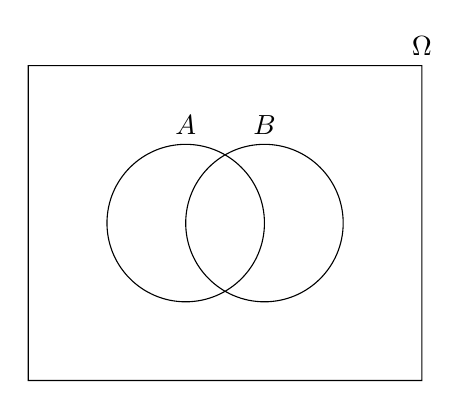
\begin{tikzpicture}[fill=white]
% left hand
\scope
\clip (-2,-2) rectangle (2,2)
      (1,0) circle (1);
\fill[white] (0,0) circle (1);
\endscope
% right hand
\scope
\clip (-2,-2) rectangle (2,2)
      (0,0) circle (1);
\fill[white] (1,0) circle (1);
\endscope
% outline
\draw (0,0) circle (1) (0,1)  node [text=black,above] {$A$}
      (1,0) circle (1) (1,1)  node [text=black,above] {$B$}
      (-2,-2) rectangle (3,2) node [text=black,above] {$\Omega$};
\end{tikzpicture} & &
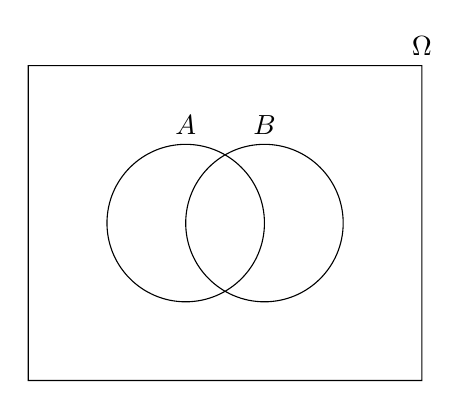
\begin{tikzpicture}[fill=white]
% left hand
\scope
\clip (-2,-2) rectangle (2,2)
      (1,0) circle (1);
\fill[white] (0,0) circle (1);
\endscope
% right hand
\scope
\clip (-2,-2) rectangle (2,2)
      (0,0) circle (1);
\fill[white] (1,0) circle (1);
\endscope
% outline
\draw (0,0) circle (1) (0,1)  node [text=black,above] {$A$}
      (1,0) circle (1) (1,1)  node [text=black,above] {$B$}
      (-2,-2) rectangle (3,2) node [text=black,above] {$\Omega$};
\end{tikzpicture} \\
 &  & \\
  &  & \\
(c) $A \cap B$ & & (d) $A-B$\\
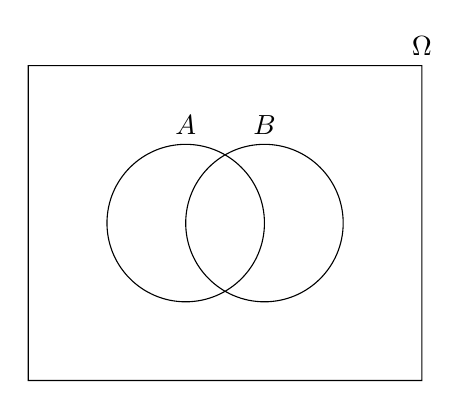
\begin{tikzpicture}[fill=white]
% left hand
\scope
\clip (-2,-2) rectangle (2,2)
      (1,0) circle (1);
\fill[white] (0,0) circle (1);
\endscope
% right hand
\scope
\clip (-2,-2) rectangle (2,2)
      (0,0) circle (1);
\fill[white] (1,0) circle (1);
\endscope
% outline
\draw (0,0) circle (1) (0,1)  node [text=black,above] {$A$}
      (1,0) circle (1) (1,1)  node [text=black,above] {$B$}
      (-2,-2) rectangle (3,2) node [text=black,above] {$\Omega$};
\end{tikzpicture} & &
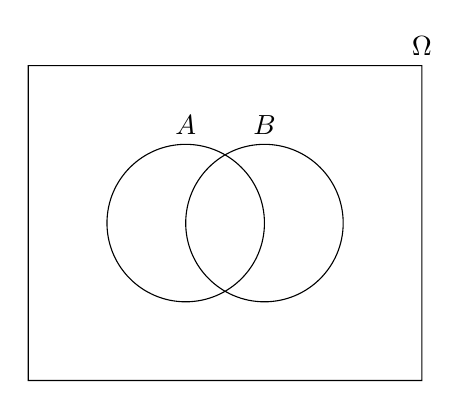
\begin{tikzpicture}[fill=white]
% left hand
\scope
\clip (-2,-2) rectangle (2,2)
      (1,0) circle (1);
\fill[white] (0,0) circle (1);
\endscope
% right hand
\scope
\clip (-2,-2) rectangle (2,2)
      (0,0) circle (1);
\fill[white] (1,0) circle (1);
\endscope
% outline
\draw (0,0) circle (1) (0,1)  node [text=black,above] {$A$}
      (1,0) circle (1) (1,1)  node [text=black,above] {$B$}
      (-2,-2) rectangle (3,2) node [text=black,above] {$\Omega$};
\end{tikzpicture}
\end{tabular}
\ee

%\clearpage

%\pagebegin{Important Venn Diagrams}


%\begin{center}
%\includegraphics[width=3in]{03/03-venn_student.jpg} \ \ \ \ \ 
%\includegraphics[width=3in]{03/03-web_venn.png}
%\end{center}

%\vspace{0.75in}

%\begin{center}
%\includegraphics[width=3in]{03/03-venn_drwho.jpg} \ \ \ \ \ \ 
%\includegraphics[width=2in]{03/03-denzel_venn.png}
%\end{center}


\clearpage
\pagebegin{Probability Rules}

We can generalize the calculations from the previous case study on vitamin A and childhood morbidity to obtain the following results:

\bbox
\begin{theorem}
Let $A$ and $B$ denote two events in sample space $\Omega$, then
\bi
\ii \textbf{\alert{Additive rule}}: $P(A \cup B) = P(A) + P(B) - P(A \cap B)$.
\ii \textbf{\alert{Bayes' Theorem}}: $\dsty P(B | A) = \frac{P(A \cap B)}{P(A)}$
\ii \textbf{\alert{Multiplicative rule}}: $P(A \cap B) = P(A) \cdot P(B | A)$
\ii \textbf{\alert{Complement rule}}: $P(A^C) = 1 - P(A)$
\ei
\end{theorem}
\ebox

\bb[resume] 
\ii When a customer purchases a new car, they are presented with a menu of options such as heated steering wheel, parking assistant, satellite radio, etc. The two most popular options on a certain type of new car are a sunroof (denoted $S$) and heated seats (denoted by $H$). Answer the following questions if we know that 
\[ P(S) = 0.6, \quad P(H) = 0.45,\mbox{ and} \quad P(H | S ) = 0.65 \] \label{q:cars}

\bb
\ii Interpret the practical meaning of $P(H | S ) = 0.65$. \vfill
\ii Compute $P(H^C)$ and interpret the meaning. \vfill
\ii Compute $P(S \cap H)$ and interpret the meaning. \vfill
\ii Compute $P(S | H)$ and interpret the meaning. \vfill
\ee
\ee

\clearpage

\pagebegin{Independent Events}

Often in statistics we want to investigate questions such as:
\bi
\ii Is a newly developed vaccine effective?
\ii Do certain sentencing laws have an effect on crime rates?
\ii Did increasing the minimum wage for fast food workers effect fast food prices?
\ii \textbf{Does the occurrence of one event (getting a sunroof) effect the likelihood that another event (heated seats) occurs?}
\ei

\bb[resume]
\ii In the car option example in question \ref{q:cars}, we know that  $P(S) = 0.6$, $P(H) = 0.45$, and $P(H | S ) = 0.65$. Based on this information, \textbf{if a customer has purchased the sunroof option, are they more, less, or equally likely to get the heated seats option?} Explain how you determined your answer.

\vfill


\ee

\bbox
\begin{definition}\label{def:ind}
Two events $A$ and $B$ are \textbf{\alert{independent}} if the occurrence of one has no effect on the occurrence of the other:

\vspace{0.5in}

%\[ P(B) = P(B | A) \quad \mbox{or} \quad P(A) = P(A | B), \]
\alert{Special case:} If events $A$ and $B$ are independent events then we have $P(A \cap B) = P(A)P(B)$.
\end{definition}
\ebox

\bb[resume]

\ii A person flips a fair coin and stops once they get at least one head and one tail. What is the probability that it takes exactly four flips to get exactly one head and one tail.

\vfill

\ee

\clearpage

%\ii Assume that the overall risk of breast cancer in a 45 year old woman is 1\%. The mammogram test used to screen for
%breast cancer is 90\% \textbf{sensitive}, meaning the test gives a correct positive 90\% of the time. We also know that the mammogram test is 95\% \textbf{specific}, meaning the test gives a correct negative 95\% of the time.\label{medical}
%%Let $D$ denote the event that a 45 year old woman has breast cancer (so $D^C$ is the event she is cancer free). Let $X$ denote the event that the mammogram result is positive for breast cancer (so $X^C$ is the event the screening comes back negative). 
%%\begin{multicols}{2}

%\begin{center}
%\begin{tabular}{c||c|c||c}
%\hline
%\  & $X$, Test Positive & $X^C$, Test negative & Total\\
%\hline
%\hline
%$D$, does have breast cancer &  &  & \\
%\hline
%$D^C$, does NOT have breast cancer &  &  & \\
%\hline
%\hline
%Total &  &  & $100$
%\end{tabular}
%\end{center}

%%\columnbreak
%\bb
%\ii For example, if 100 woman take a mammogram test, fill in the rest of the blanks to complete the \textbf{contingency table} above. \ss
%\ii Are events $D$ and $X$ independent? Show or explain why or why not? \vfill
%%\ee
%%\end{multicols}
%%\bb
%%\addtocounter{enumii}{2}
%\ii What is the probability that a randomly selected 45 year old woman has breast cancer and has a positive test result? \vfill
%\ii What is the probability that a randomly selected 45 year old woman has breast cancer or has a positive test result? \vfill
%\ii You are a doctor who has a 45 year old female patient whose mammogram result is positive. How likely is this patient
%to actually have breast cancer?\vfill
%\ee
%\ee

%\bb[resume]
%\ii According to Lord Mersey's original report to the British Parliament in 1912, there were a total of $2,\!224$ passengers and crew aboard the Titanic when it sank, resulting in the death of $1,\!513$ passengers and crew.  The \textbf{contingency} (or two-way) table shows the passenger breakdown. Let $A_1$, $A_2$, $A_3$ and $A_4$ be the event a randomly selected person onboard the Titanic is first-class, second-class, third-class or crew. Let $S$ be the event the passenger survived.

%\begin{multicols}{2}

%\begin{center}
%\begin{tabular}{c||c|c||c}
%\hline
%\  & Survived & Died & Total\\
%\hline
%\hline
%1st & 203 & 122 & 325\\
%\hline
%2nd & 118 & 167 & 285\\
%\hline
%3rd & 178 & 528 & 706\\
%\hline
%Crew & 212 & 696 & 908\\
%\hline
%\hline
%Total & 711 & 1,\!513 & 2,\!224
%\end{tabular}
%\end{center}

%\columnbreak

%\bb
%%\ii What is the probability that a randomly selected passenger on the Titanic survived?
%\ii Are events $A_2$ and $S$ independent? Show why or why not?
%\ee
%\end{multicols}
%\bb
%\addtocounter{enumii}{1}
%\ii What is the probability that a randomly selected passenger survived and was second-class? \vfill
%\ii What is the probability that a randomly selected passenger survived or was second-class? \vfill
%\ii What is the probability that a randomly selected passenger survived given that we know the passenger was second-class? \vfill
%\ii What is the probability that a randomly selected passenger was second-class class given that we know the passenger survived? \vfill
%\ee
%\ee

%\clearpage

%\pagebegin{Conditional Probabilities}

%\bb[resume]
%\ii Based on your work in \ref{medical}, fill in the blank in definition \ref{def:conditional} below.
%\ee

%\bbox
%\begin{definition}\label{def:conditional}
%If $P(B) >0$, then the \textbf{conditional probability} of $A$ given $B$ is denoted
%\[ P(A \mid B) = \rule{0.2\tw}{0.5pt}.\]
%\end{definition}
%\ebox

%\bb[resume]
%\ii Complete the lemma by filling each blank with one of the following: $P(A \mid B)$, $P(B \mid A)$, $P(A \cap B)$, $P(A)$, or $P(B)$.
%\begin{lemma}\label{lemma:conditional}
%From definition \ref{def:conditional} it follows that
%\bi
%\ii $P(A \cap B) = $ \rule{0.1\tw}{0.5pt} $\cdot P(B) = $ \rule{0.1\tw}{0.5pt} $\cdot P(A)$. \bs
%\ii If $A$ and $B$ are independent events, then $P(A \mid B) = $ \rule{0.1\tw}{0.5pt} .
%\ei
%\end{lemma}
%\ee


\clearpage

\pagebegin{Probability Distributions}

\bbox
\begin{definition}
Two events $A$ and $B$ are \textbf{disjoint} (or \textbf{mutually exclusive}) if they cannot occur at the same time, and therefore $P(A \cap B) = 0$.
\smallskip

\alert{Special case:} If events $A$ and $B$ are disjoint then we have $P(A \cup B) = P(A)+P(B)$.
\end{definition}
\ebox

%\bb[resume]
%\ii Returning to the job applicants example in \ref{applicants}, give an example of:\label{disjoint}
%\bb
%\ii Three different events that are disjoint from one another.\label{aredisjoint} \vfill
%\ii Two different events that are NOT disjoint from one another.\label{notdisjoint} \vfill
%\ee
%\ee


\bb[resume]
%\ii Do the three events you identified in \ref{aredisjoint} form a partition of the sample space $S$ in \ref{applicants}? Show or explain why or why not.
\ii In the options for a new car example in question \ref{q:cars}, are events $H$ and $S$ mutually exclusive? Why or why not? \vfill

\ee

\bbox
\begin{definition}\label{def:prob-dist}
A function $P$ that assigns a real number $P(A)$ to each event $A$ is a \textbf{probability distribution} or a \textbf{probability measure} if it satisfies the following three axioms:
\bb
\ii $P(A) \geq$ \rule{0.1\tw}{0.5pt} for all $A$. \bs
\ii $P(\mbox{full sample space})=P(\Omega) =$ \rule{0.1\tw}{0.5pt} . \bs
\ii If $A$ and $B$ are disjoint, then
\[ P \left( A \cup B \right) = \mbox{\rule{0.25\tw}{0.5pt}}.\]
\ee
\end{definition}
\ebox

%\bb[resume]
%\ii Prove that as a result of definition \ref{def:prob-dist} it follows that $P(A) = 1-P(A^C)$.'\vfill \vspace{1in}

%\ii A fair coin is tossed until we get exactly two heads. What is $\Omega$, the sample space? What is the subset, call it $A$, that corresponds to requiring exactly 4 tosses? What is $A^C$?

%\ee

\clearpage

\pagebegin{OPTIONAL: Counting}


\bb[resume]
\ii 5 people have volunteered to work on a committee. The committee will consist of a total of three people. How many different committees of 3 people can be formed from the 5 volunteers? \vfill
\ee


\bbox
We often need to count the number of ways of choosing $k$ items out of $n$ possible items. You may recall this is often called \textbf{$\mathbf{n}$ choose $\mathbf{k}$} and is denoted as

\[ \left( \begin{array}{c} n \\ k \end{array}\right) = \frac{n!}{k!(n-k)!}.\]
\ebox

\bb[resume]
\ii BONUS: Suppose $n$ people are in a room. What is the probability that there is at least one pair of people that have the same birthday? \textit{Hint: Let $A$ be the event there is no match. Calculate $P(A)$, and then find $P(A^C)$.} %\vfill

\vfill

\ee



%\clearpage

\begin{center}
\includegraphics[width=5in]{03/tyson-tweet.png}
\end{center}
\bs

%\bbox
%\bi 
%\ii A \textbf{statistical experiment or observation} is any random activity that results in a definite outcome.
%\ii The \textbf{sample space} $\Omega$ is the set of all possible outcomes of an experiment.
%\ii An \textbf{outcome, realization or elements}, $\omega$, is a result from an experiment or observation.
%\ii An \textbf{event}, $A$, is a collection of one or more outcomes from an experiment or observation.
%\ei
%\ebox

%\bb
%\ii There are two people in a room. You ask each person what is their birthday (excluding the year).
%\bb
%\ii List several outcomes in the sample space. How many outcomes are in the sample space $\Omega$? \vfill
%\ii Let $M$ denote the event that the two people have the same birthday. How many outcomes are in this event? \vfill
%\ee

%\ii At the end of the semester I randomly select a student in the course and observe their average for the semester.
%\bb
%\ii What is the sample space $\Omega$? \vfill
%\ii What is the event that a student passes the course? \vfill
%\ee

%\ii If possible, give an example of an \textbf{infinite sample space} that is \textbf{discrete}? \vfill

%\ee


\clearpage

\pagebegin{OPTIONAL: Bayes' Theorem}

\bbox
\begin{definition}
A \textbf{partition} of a space $\Omega$ is a collection of disjoint sets such that $\dsty \bigcup_{i=1}^{\infty} A_i = \Omega$.
\end{definition}
\ebox



%%%%%%%%%%%%%%
%% Move elsewhere
%%%%%%%%%%%%%%
\bb[resume]

\ii Fill in the blank to complete theorem \ref{thm:total-prob} below and explain (in words, pictures, or equations) how you determined your answer.

\begin{multicols}{2}

\includegraphics[width=0.4\tw]{03/03-venn-totalprob.jpg}

\columnbreak
\bbox
\begin{theorem}{Law of Total Probability}\label{thm:total-prob}
Let $A_1$, $A_2$, $\ldots , A_k$ be a partition of $\Omega$. Then for any event $B$,
\[ P(B) = \sum_{i=1}^k \rule{0.2\tw}{0.5pt}.\]
\end{theorem}
\ebox

\end{multicols}
\ee

%%%%%%%%%%%%%%
%% Move elsewhere
%%%%%%%%%%%%%%


\clearpage

\bbox
\begin{theorem}{Bayes' Theorem}\label{thm:bayes}
Let $A_1$, $A_2$, $\ldots , A_k$ be a partition of $\Omega$ such that $P(A_i)>0$ for each $i$. If $B$ is any event with $P(B)>0$, then for each $i=1, \ldots k$, we have
Then for any event $B$,
\[ P(A_i \mid B) = \frac{P(A_i \cap B) }{P(B)} = \frac{P(B \mid A_i) P(A_i)}{\sum_{j=1}^k P(B \mid A_j)P(A_j)}.\]
\end{theorem}
\ebox

\bb[resume]
\ii Suppose that 30\% of computers run Mac, 50\% use PC, and 20\% use Linux. A computer virus is
created by hackers, and suppose that  65\% of Mac, 82\% of PC, and 50\% of Linux computers get the virus.
\bb
\ii What is the probability that a randomly selected computer has the virus? \vfill
\ii What is the probability that a randomly selected computer is PC given that the computer is infected by the virus?\vfill \vspace{1in}
\ee
\ee

%\ii Recall the Monty Hall problem. Imagine you are playing the game and initially select door number 1. The game show host than opens one of the other doors (door 2 or door 3) to reveal one of the goats. Let $W$ denote the event the contest wins after making their decision (either \textit{Switch} or \textit{Stay}).
%\bb
%\ii Calculate $P(W \mid \mbox{\textit{Stay}})$. \vfill
%\ii Calculate $P(W \mid \mbox{\textit{Switch}})$. \vfill
%\ii What is the best strategy?  \vfill
%\ii Are $W$ and \textit{Stay} independent events? Mutually exclusive events? \vfill
%\ee
  %Chapter 2 Discrete RV
%%UNIT 1: QUALITATIVE AND GRAPHICAL APPROACHES
% Is first part of original 01.tex
%%%%%%%%%%%%%%%%%%%%%%%%%%%
%%%% Put the following at the top of each .tex file  %
\pagestyle{fancy}
\renewcommand{\theUnit}{2}
\ifthenelse{\isundefined{\UnitPageNumbers}}{}{\setcounter{page}{1}}
\rhead{Carlton and Devore Chapter \theUnit: Discrete Random Variables}
\lhead{Math 3382: Statistical Theory}
%\lhead{\includegraphics[width=1.25cm]{CUDenver-Logo.png}}
\rfoot{\mypage}
\cfoot{\includegraphics[width=2.25cm]{CUDenver-Logo-coverpage.png}}
\lfoot{Adam Spiegler}
\fancypagestyle{firstfooter}{\footskip = 50pt}
\renewcommand{\footrulewidth}{.4pt}
%%%%%%%%%%%%%%%%%%%%%%%%%%%
\vspace*{-20pt} \thispagestyle{firstfooter}

\pagebegin{Introduction to Random Variables}

Suppose a company knows that 1\% of the lithium batteries they manufacture are defective.  The manufacturer sends a shipment of 10 batteries to one of their clients. How likely is it that none of the batteries are defective? How can we connect the data to the concepts of sample spaces and events to answer this question? This link can be made using \textbf{\alert{random variables}}:

\begin{tcolorbox}
\begin{definition}\label{def:rv}
A \textbf{\alert{random variable}} is a mapping
\[ X: \Omega \to \mathbb{R} \]
that assigns a real number $X(\omega)$ to each outcome $\omega \in \Omega$.
\end{definition}
\end{tcolorbox}

For example, the random variable $X$ could map an outcome in which 10 batteries are selected at random to a number corresponding to how many batteries in the sample are not defective, denoted $G$ for good. For instance if $\omega = DDGGGGGGGG$, then $X(DDGGGGGGGG)=8$. We can calculate the probability that $X=10$ (none are defective) using independence of events:
\[ P(X=10) = P(G)P(G) \cdots P(G) = (P(G))^{10} = (0.99)^{10} \approx 0.9044.\]

\bb
\ii A student takes a 3 question quiz. Each of the 3 questions is multiple choice with 4 possible answer choices. Let the random variable $X$ be the number of correct guesses out of the 3 questions.\label{quiz}
\bb
\ii What is the sample space $\Omega$?\label{quizA}
\vspace{0.75in}
\ii Compute $P(X=0)$, how likely is it that the student gets none of the questions correct?
\vspace{0.75in}
\ii Fill in the empty entries in table below

\begin{center}
\begin{tabular}{|c|c|c|c|c|}
\hline
$x$ & \hspace{0.25in} 0  \hspace{0.25in} &  \hspace{0.25in} 1  \hspace{0.25in} &  \hspace{0.25in} 2  \hspace{0.25in} &  \hspace{0.25in} 3  \hspace{0.25in} \\
\hline
 & & & & \\
$P(X=x)$ & & & & \\
 & & & & \\
\hline
\end{tabular}
\end{center}

\ii Compute $P(X \leq 1)$ and interpret the practical meaning of this value.
\ee
\ee

\clearpage

\pagebegin{Distribution Functions}

\begin{tcolorbox}
\begin{definition}\label{def:pmf}
If $X$ is a \textbf{\alert{discrete}} random variable, we define the probability function or \textbf{\alert{probability distribution}} or \textbf{\alert{probability mass function (pmf)}}
for $X$ by
\[ p(x) = P(X=x) .\]
\end{definition}

\vspace{-0.25in}

\begin{definition}\label{def:cdf1}
If $X$ is a random variable, we define the \textbf{\alert{cumulative distribution function (cdf)}} as the function
\[ F(x)=P(X \leq x) = \sum_{k=\mbox{\scriptsize{min value}}}^x p(k) .\]
\end{definition}
\end{tcolorbox}

% Below is a geogebra interactive thing with binomial
% https://www.geogebra.org/m/GyYQWWNX

\bb[resume]
\ii Sketch the pmf and cdf for the random variable $X$ (number of correct guesses on the 3 question quiz) in question \ref{quiz}. Be sure to label the tickmarks on the vertical axes with an appropriate scale.

\begin{center}
\begin{tabular}{ll}
\includegraphics[width=0.3\tw]{04/04-blank-pmf.png} \hspace{1in} &
\includegraphics[width=0.3\tw]{04/04-blank-cdf.png} \\
Sketch the pmf, $p(x)$. & Sketch the cdf, $F(x)$\\
\end{tabular}
\end{center}

\ii Let $X$ is a discrete random variable with pmf and cdf denoted $p(x)$ and $F(x)$, respectively. Determine if each statement is True or False.
\begin{tasks}[counter-format = {(tsk[a])},label-offset = {0.8em},label-format = {\color{black}}](2)
\task $0 \leq p(x) \leq 1$ for all $x$.
\task $0 \leq F(x) \leq 1$ for all $x$. \vspace{0.45in}
\task $\dsty \sum_{\mbox{all $x$}} p(x) = 1$.
\task $\dsty \sum_{\mbox{all $x$}} F(x) = 1$. \vspace{0.45in}
\task $\dsty \lim_{x \to \infty} p(x) = 1$.
\task $\dsty \lim_{x \to \infty} F(x) = 1$. \vspace{0.45in}
\task The pmf must be a nondecreasing function.
\task The cdf must be a nondecreasing function. \vspace{0.45in}
\end{tasks}
\ee

\clearpage

\pagebegin{Expected Value and Variance}

\begin{tcolorbox}
\begin{definition}\label{def:expected}
The average or \textbf{\alert{expected value}} for a discrete random variable $X$ is denote $E(X)$ or $\mu$ and computed using the formula
\[ E(X) = \mu =  \sum_x \left( x \cdot p(x) \right) = \sum_x \left( x \cdot P(X=x) \right). \]
\end{definition}
\vspace{-0.5in}

\begin{definition}\label{def:variance}
The \textbf{\alert{variance}} for a discrete random variable $X$ is one common way to measure how spread out (in relation to the expected value) are the values of $X$. The variance is denoted $\Var(X)$ or $\sigma^2$ and computed using the formula
\[ \Var(X) = \sigma^2 =  \sum_x \left( (x-\mu)^2 \cdot p(x) \right) = \sum_x \left( (x-\mu)^2 \cdot P(X=x) \right). \]
\end{definition}
\vspace{-0.5in}

\begin{definition}\label{def:variance}
The \textbf{\alert{standard deviation}} for a discrete random variable $X$ is the square root of the variance and is denoted by $\sigma$. It more or less measures the average of the distances for each value of $X$ from the mean $\mu$.
\[ \mbox{SD}(X) = \sigma =  \sqrt{\Var(X)}. \]
\end{definition}


\end{tcolorbox}

\bb[resume]
\ii Using properties of the pmf, $p(x)$, show that \label{var-prop}
\begin{tcolorbox}
\[ \Var(X) = E(X^2)  - \mu^2  \]
\end{tcolorbox}

\vspace{0.5in}
\vfill

\ii A charity is running a raffle as afundraiser. They offer one grand prize of \$$500$, two second prizes of \$$100$ each, and ten third prizes of \$$20$ each. They plan to sell $1,\!000$ tickets each at a price of \$$2$. Let $X$ denote the amount of money won by a lottery ticket.\label{lottery}
\bb
\ii Fill in the values of $x$ and $p(x)$ in the table below.\medskip

\begin{center}
\begin{tabular}{|c||c|c|c|c|}
\hline
$x$ &  \hspace{0.5in}  &  \hspace{0.5in}  &  \hspace{0.5in}  &  \hspace{0.5in} \\
\hline
$p(x)$ & & & &  \\
\hline
\end{tabular}
\end{center} \medskip
%\begin{center}
%\begin{tabular}{c|c|c}
%x & \hspace{0.5in} P(x) \hspace{0.5in} & \hspace{1in} $(x-\mu)^2$ \hspace{1in}  \\
%\hline
 % & & \\
 %   & & \\
%\hline
%  & & \\
 %   & & \\
%\hline
%  & & \\
 %   & & \\
%\hline
%  & & \\
 %   & & \\
%\end{tabular}
%\end{center}  \medskip

\ii Calculate $E(X)$ and $\Var(X)$.
\ee
\ee
\vfill
  %Chapter 3 Continuous RV
%%UNIT 1: QUALITATIVE AND GRAPHICAL APPROACHES
% Is first part of original 01.tex
%%%%%%%%%%%%%%%%%%%%%%%%%%%
%%%% Put the following at the top of each .tex file  %
\pagestyle{fancy}
\renewcommand{\theUnit}{2}
\ifthenelse{\isundefined{\UnitPageNumbers}}{}{\setcounter{page}{1}}
\rhead{Carlton and Devore Chapter \theUnit: Discrete Random Variables}
\lhead{Math 3382: Statistical Theory}
%\lhead{\includegraphics[width=1.25cm]{CUDenver-Logo.png}}
\rfoot{\mypage}
\cfoot{\includegraphics[width=2.25cm]{CUDenver-Logo-coverpage.png}}
\lfoot{Adam Spiegler}
\fancypagestyle{firstfooter}{\footskip = 50pt}
\renewcommand{\footrulewidth}{.4pt}
%%%%%%%%%%%%%%%%%%%%%%%%%%%
\vspace*{-20pt} \thispagestyle{firstfooter}

\pagebegin{Discrete Random Variables}

\bb
\ii Suppose a company knows that 1\% of the lithium batteries they manufacture are defective.  The manufacturer sends a shipment of 10 batteries to one of their clients. Let the random variable $X$ denote the number of good (not defective) batteries in the shipment. How likely is it that exactly two of the batteries are defective? \label{q:batteries}

\bb
\ii What is the probability of getting the outcome $GGGGGGGGDD$? Note $G$ and $D$ denote good and defective batteries, respectively. \vfill
\ii How many outcomes are in the event exactly 2 out of 10 batteries are defective? \vfill
\ii Calculate $P(X=8)$. \vfill
\ee

\ii Generalize the result in the previous example. If you repeat $n$ trials which are independent from one another, and each has the same probability of success, $p$, what is the probability of getting exactly $s$ successes out of $n$ trials? \bigskip

$\dsty f(s) = P(X=s) =$   \bigskip

\ii How many good batteries would you expect to receive if you had a shipment of 100 batteries (where it is known that $1$\% of all batteries are defective)? If you received a shipment of 200 batteries? A shipment of 10 batteries? \vfill

\ii Write a general formula for the expected number of successes when $n$ trials are repeated with probability of success $p$ in each trial. \vfill

\ee

\clearpage

\pagebegin{Binomial Distributions}

\begin{tcolorbox}
\bi
\ii A \textbf{\colorb{Bernoulli trial}} is an experiment that has \textbf{\colorb{exactly two possible outcomes}}:
\bi
\ii[$\circ$] The probability that the outcome of a trial is a \colorb{success} ($X=1$ ) is denoted \colorb{$p$}.
\ii[$\circ$] Otherwise, the probability of a \colorr{failure} ($X=0$ ) is \colorr{$q=1-p$}.
\ii[$\circ$] $X$ has a \textbf{\colorb{Bernoulli Distribution}} with probability mass function
\[ f(x) = p^x(1-p)^{1-x} \ \ , \mbox{for } x \in \left\{ 0, 1 \right\}.\]
\ei

\ii Let random variable $X$ be the number of successes out of $n$ trials, where \colorb{each trial is identical and independent}. 
\bi
\ii[$\circ$] $X$ has a \textbf{\colorb{Binomial Distribution}}, written $X \sim \mbox{Binomial}(n,p)$.
\ii[$\circ$] The probability mass function is
\[ f(x) = \left\{ \begin{array}{ll} \left( \begin{array}{c} n\\ x \end{array} \right) p^x(1-p)^{n-x} \ \ & \mbox{for } x =0,1,2, \ldots , n\\
 & \\
0 \ \ & \mbox{otherwise} \end{array} \right. .\]
\ii[$\circ$] The expected value can be calculated with the shortcut \colorb{$E(X) = np$}.
\ii[$\circ$] The variance can be calculated with the shortcut \colorb{$\Var(X) = npq$}.
\ei
\ei
\ebox

\medskip

\begin{tcolorbox}
In R, the we can use the functions:
\bi
\ii \colorb{dbinom($x$, $n$, $p$)} calculates the probability of \colorb{exactly $x$ success} out $n$ trials, \colorb{$P(X=x)$}. 
\ii \colorr{pbinom($x$, $n$, $p$)} calculates the probability of \colorr{at most $x$ success} out $n$ trials, \colorr{$P(X \leq x)$}. 
\ei
\end{tcolorbox}

\bb[resume]
\ii Consider the lithium battery example from question \ref{q:batteries}. Write a command in R that computes the given probability.
\bb
\ii Exactly 7 batteries are good. \vfill
\ii At most 8 batteries are good. \vfill
\ii At most 4 batteries are defective. \vfill
\ee
\ee

\clearpage

\pagebegin{Equally Likely Outcomes}

\bb[resume]
\ii Let $X$ be the value of the result of rolling a fair six-sided die.
\bb
\ii Write out the probability mass function $f(x)$. \vfill
\ii What is the expected value of rolling a fair-six sided die? \vfill
\ee
\ee


\bbox
Let $X$ be a discrete random variable with $k$ different outcomes that each have the same likelihood of occurring.
\bi
\ii $X$ has a \textbf{\colorb{uniform distribution}} on $\left\{ 1, 2, 3, \ldots , k \right\}$
\ii The probability mass function is 
\[ f(x) = \left\{ \begin{array}{ll} \frac{1}{k} \ \ & \mbox{for } x = 1, 2, \ldots,  k\\
0 \ \ & \mbox{otherwise} \end{array} \right. .\]
\ii The expected value is $E(X) = \frac{k+1}{2}$.
\ii The variance is $\Var(X) = \frac{k^2-1}{12}$.
\ei 
\ebox

\bb[resume]
\ii A sports marketer for the Denver Nuggets randomly calls people in the Denver area until she encounters someone who attended a Nuggets' game. What is the probability the market encounters $7$ people who did not attend a game before the first success when it is known that 10\% of the population attended a game last season? \vfill
\ee

\clearpage

\pagebegin{Number of Failures Before First Success}


\bbox
If we repeat a Bernoulli trial that has probability of success $p$ for each trial, we can \colorb{count the number of failures, $X$, that occur before the first success.}
\bi
\ii $X$ has a \textbf{\colorb{Geometric Distribution}}, written $X \sim \mbox{Geom}(p)$.
\ii The probability mass function is $\dsty f(x) = q^xp$ for $x \in \lbrace 0, 1, \ldots \rbrace$.
\ii The expected value is $\mu=E(X) = \frac{q}{p}$.
\ii The variance is $\sigma^2 = \Var(X) = \frac{q}{p^2}$.
\ei

\medskip

In R, the we can use the functions:
\bi
\ii \colorb{dgeom($x$, $p$)} calculates the probability of \colorb{exactly $x$ failures} before first success. 
\ii \colorr{pgeom($x$, $p$)} calculates the probability of \colorr{at most $x$ failures} before first success.
\ii There is no fixed number of trials $n$.
\ei 
\ebox

\pagebegin{Number of Occurrences in a Fixed Time Period}

\bbox
The \textbf{\colorb{Poisson distribution}} applies when the average frequency of occurrences in a given time period is known, and each occurrence is independent the others. Let $X$ denote \colorb{the number of occurrences in the given time period}.
\bi
\ii $X \sim \mbox{Poisson}(\lambda)$, where $\lambda$ denotes the mean number of occurrences in the given time.
\ii The probability mass function is $\dsty f(x) = e^{-\lambda} \frac{\lambda^x}{x!}$ for $x \in \lbrace 0, 1, 2, \ldots \rbrace$.
\ii The expected value is $\mu = E(X) = \lambda$.
\ii The variance is $\sigma^2 = \Var(X) = \lambda$ (same as the expected value).
\ei 

\medskip

In R, the we can use the functions:
\bi
\ii \colorb{dpois($x$, $\lambda$)} calculates the probability of \colorb{exactly $x$ occurrences} in the given time.
\ii \colorr{ppois($x$, $\lambda$)} calculates the probability of \colorr{at most $x$ occurrences} in the given time.
\ei %\bigskip
\ebox

\bb[resume]
\ii If there are twelve cars crossing a bridge per minute on average, find the probability of having seventeen or more cars crossing the bridge in a particular minute.
\ee

\vfill

\clearpage

\pagebegin{Practice}

\bb[resume]
\ii For each situation, identify which distribution best describes the distribution of the random variable. Then use a probability distribution function to calculate the probability.
\bb
\ii A online retailer sells an average of 5 big screen TV's on a given day. What is the probability they sell 9 TV's in a day? \vfill
\ii It is known that 3\% of airbags manufactured by a certain car company are defective. What is the probability that the first defective air bag occurs when the fifth item is inspected? \vfill
\ii Recently, a nurse commented that when a patient calls the medical advice line claiming to have the flu, the chance that he or she truly has the flu (and not just a nasty cold) is only about 4\%. Of the next 25 patients calling in claiming to have the flu, what is the probability that exactly 4 patients will have the flu? \vfill
\ee
\ee
  %Joint and Marginal: Sections 4.2 and 5.2; more closely Stat with App 4.1
%%%UNIT 1: QUALITATIVE AND GRAPHICAL APPROACHES
% Is first part of original 01.tex
%%%%%%%%%%%%%%%%%%%%%%%%%%%
%%%% Put the following at the top of each .tex file  %
\pagestyle{fancy}
\renewcommand{\theUnit}{3}
\ifthenelse{\isundefined{\UnitPageNumbers}}{}{\setcounter{page}{1}}
\rhead{Carlton and Devore Chapter \theUnit: Continuous Random Variables}
\lhead{Math 3382: Statistical Theory}
%\lhead{\includegraphics[width=1.25cm]{CUDenver-Logo.png}}
\rfoot{\mypage}
\cfoot{\includegraphics[width=2.25cm]{CUDenver-Logo-coverpage.png}}
\lfoot{Adam Spiegler}
\fancypagestyle{firstfooter}{\footskip = 50pt}
\renewcommand{\footrulewidth}{.4pt}
%%%%%%%%%%%%%%%%%%%%%%%%%%%
\vspace*{-20pt} \thispagestyle{firstfooter}

\pagebegin{Introduction to Continuous Random Variables}

A manufacturer of lithium batteries measures the weight of each box they ship out to customers. Let $X$ denote the weight (in pounds) of a randomly selected shipment. It is possible that $X=8$ or $X=9$, but the weight could potentially be any value (greater than 0) such as $8.3671$ pounds if they want to be really precise. Recall the previous definition of a random variable below.

\begin{tcolorbox}
\begin{definition}\label{def:crv}
A \textbf{\colorb{random variable}} is a mapping
\[ X: \Omega \to \mathbb{R} \]
that assigns a real number $X(\omega)$ to each outcome $\omega \in \Omega$.
\end{definition}

\bi
\ii With a discrete random variable, the sample space is mapped to the integers (or a subset of the integers).
\ii With a continuous random variable, the sample space is mapped to an interval of values in $\mathbb{R}$.
\ei

\end{tcolorbox}

\bb
\begin{multicols}{2}

\ii Imagine the GPA distribution for all students at a university follows a \textbf{\colorb{uniform distribution}} with GPA's 
of 0 and 4 being the smallest and largest GPA's possible. \label{gpa-uniform}

\bb
\ii Write a formula for probability density function $f_X(x)$ for the uniform distribution. \vspace{0.5in}
\ii What proportion of students earned a GPA between $3$ and $3.5$?
\ee

\columnbreak

\begin{center}
\includegraphics[width=0.45\tw]{06/06gpa-unif.pdf}
\end{center}

\end{multicols} \vspace{0.5in}

\begin{multicols}{2}
\ii The graph of $f_X(x)$ below shows the probability density function for the GPA's of all students at a university.\label{gpa-v}

\bb
\ii What proportion of students at the university have a GPA between 3 and 4? \vspace{0.5in}
\ii What proportion of students at the university have a GPA between 1 and 3?
\ee

\columnbreak

\includegraphics[width=0.5\tw]{06/06gpa-v.pdf}

\end{multicols} \vspace{0.5in}

\ee

\clearpage

\pagebegin{Probability Distributions}

\begin{tcolorbox}
\begin{multicols}{2}

\begin{definition}\label{def:pdf}
If $X$ is a \textbf{continuous} random variable, the \textbf{\colorb{probability density function (pdf)}}, denoted $f(x)$ satisfies the following properties:
\bi
\ii $f(x) \geq 0$ for all $x$,
\ii $\dsty \int_{-\infty}^{\infty} f(x) = 1$, and 
\ii $\dsty P(a < x < b) = \int_a^b f(x) \, dx$
\ei
\end{definition}

\columnbreak

\includegraphics[width=0.5\tw]{06/06area1.png}
\end{multicols}
\end{tcolorbox}

\bb
\ii The probability of a transistor failing between time $x=a$ and $x=b$ months is given by the probability density function\label{transistor}
\[ f(x) = c \int_a^b e^{-cx} \, dx.\]
\bb
\ii If the probability of failure within the first six months, $0 < x < 6$, is 10\%, set up (but do not solve) an equation to find the value of $c$? \vfill
\ii Set up (but do not evaluate) an integral to represent the probability the transistor fails within the second six months ($6<x<12$)? \vfill
\ii Interpret the meaning of $P(X \leq 9)$ and $P(X < 9)$.\vfill
\ee
 \ee

\clearpage

\begin{tcolorbox}
\begin{definition}\label{def:cdf2}
If $X$ is a \textbf{continuous} random variable, the \textbf{\colorb{cumulative distribution function (cdf)}}, denoted $F(x)$ is
\[ P(X < x) = F(x) = \int_{-\infty}^x f(t) \, dt.\]
\textbf{\colorb{In other words, $F(x)$ is an antiderivative of $f$,} and \colorr{$f(x)$ is the derivative of $F(x)$}.}
\end{definition}
\end{tcolorbox}

\bb[resume]
\begin{multicols}{2}
\ii Match the graphs of the density functions (a), (b), and (c)  with the graphs of the cumulative distribution functions I, II, and III.\label{graph-match}
\columnbreak
\includegraphics[width=0.5\tw]{06/06match.png}
\end{multicols}
\ee

%\clearpage

%\pagebegin{Cumulative Distribution Functions: Section 3.1}

%\bb[resume]
%\ii Decide if the function graphed in is a
%probability density function (pdf) or a cumulative distribution
%function (cdf).  Give reasons.  Find the value of $c$.  Sketch and
%label the other function.  (That is, sketch and label the cdf if the
%problem shows a pdf, and the pdf if the problem shows a cdf.)

%\begin{tasks}[counter-format = {(tsk[a])},label-offset = {0.8em},label-format = {\color{black}\bfseries}](2)
%\task \includegraphics[width=0.4\tw]{06/06graph1.png}
%\task \includegraphics[width=0.4\tw]{06/06graph2.png}
%\end{tasks}
%\ee

\pagebegin{Mean, Variance, and Median}

\begin{tcolorbox}
\bi
\ii The \colorb{mean} of a continuous random variable is\label{def:mean}
\[ E(X) = \mu = \int_{-\infty}^{\infty} x \cdot f(x) \, dx.\]
\ii The \colorb{variance} of a continuous random variable is\label{def:variance}
\[ \Var(X) = E(X-\mu)^2 = E(X^2) - \big( E(X) \big)^2  \ \ \ \mbox{(this can be proven similar as with discrete case)}.\] 
\ii The \colorb{median} is the value $x$ such that $P(X < x) = 0.5$. Thus to find the median we solve the following for $x$:\label{def:median}
\[ F(x) = \int_{-\infty}^x f(t) \, dt = 0.5.\]
\ei
\end{tcolorbox}

\clearpage

\pagebegin{Practice}

\bb[resume]
\ii Consider the random variable with pdf
\[ f(x) = \left\{ \begin{array}{ll} \frac{x}{8}, & \hspace{0.2in} 0 \leq x \leq 4 \\ 0, &  \hspace{0.2in} \mbox{otherwise} \end{array} \right. .\]
\bb
\ii Sketch a graph of the pdf, $f$. \vfill
\ii Give a formula for the cdf, $F$, and sketch its graph. \vspace{1in}
\ii Calculate $P(X < 1)$ and illustrate this value on both of your graphs. \vspace{1in}
\ii Calculate $E(X)$. \vspace{1in}
\ii Give the median value and illustrate this value on both of your graphs. \vfill
\ee
\ee

  %Covariance and Conditional: Section 5.4 then 5.3; more closely Stat with App 4.2 and 4.3
%%UNIT 1: QUALITATIVE AND GRAPHICAL APPROACHES
% Is first part of original 01.tex
%%%%%%%%%%%%%%%%%%%%%%%%%%%
%%%% Put the following at the top of each .tex file  %
\pagestyle{fancy}
\renewcommand{\theUnit}{3}
\ifthenelse{\isundefined{\UnitPageNumbers}}{}{\setcounter{page}{1}}
\rhead{Carlton and Devore Chapter \theUnit: Continuous Random Variables}
\lhead{Math 3382: Statistical Theory}
%\lhead{\includegraphics[width=1.25cm]{CUDenver-Logo.png}}
\rfoot{\mypage}
\cfoot{\includegraphics[width=2.25cm]{CUDenver-Logo-coverpage.png}}
\lfoot{Adam Spiegler}
\fancypagestyle{firstfooter}{\footskip = 50pt}
\renewcommand{\footrulewidth}{.4pt}
%%%%%%%%%%%%%%%%%%%%%%%%%%%
\vspace*{-20pt} \thispagestyle{firstfooter}

\pagebegin{Uniform Distributions}

\begin{tcolorbox}
Recall the \textbf{\colorb{uniform distribution}} of GPA's in problem \ref{gpa-uniform}. More generally, if a continuous random variable is uniformly distributed on the interval $\lbrack a , b \rbrack$, then
\bi
\ii The pdf is $\dsty f(x) = \left\{ \begin{array}{ll} \frac{1}{b-a}, & \hspace{12pt} a \leq x \leq b\\ 0, & \hspace{12pt} \mbox{otherwise} \end{array} \right.$.
\ii The cdf is
\[  F(x) = \left\{ \begin{array}{ll} 0, & \hspace{12pt} x<a \\ \frac{x-a}{b-a}, & \hspace{12pt} a \leq x \leq b \\ 1,  & \hspace{12pt}  x>b \end{array} \right.\]
\ii $E(X) = \frac{a+b}{2}$; $\Var(X) = \frac{(b-a)^2}{12}$; Median $=E(X) = \frac{a+b}{2}$.
\ei
\end{tcolorbox}

\pagebegin{Normal Distributions}

\begin{multicols}{2}
There are many cases where the data tends to be distributed symmetrically around a central value with no bias to the left or
right like this\footnote{Photograph by Peter Morenus in conjunction with Professor Linda Strausberg, of the University of Connecticut}:  %Subjects are University of Connecticut genetics students, females in white tops, males in dark tops}:

\columnbreak

\begin{center} \includegraphics[width=3in]{07/07people.png}\end{center}

\end{multicols}

Normal distributions arise in many settings: Heights of people, size of items produced by machines, and most importantly in statistics data sets resulting from many independent random events. \medskip

\begin{tcolorbox}

The shape of a \textbf{\colorb{normal distribution}} are determined by two parameters:
\bi
\ii The \colorr{mean, $\mu$}, is center of the distribution.
\ii The \colorr{standard deviation, $\sigma$}, tells us how wide the distribution is.
\ii If $X$ is normally distributed with mean $\mu$ and standard deviation $\sigma$, we write \colorr{$\mathbf{X \sim N(\mu, \sigma)}$}.
\ei

\end{tcolorbox}

\begin{tabular}{|c|c|}
\hline
\includegraphics[width=0.35\tw]{07/07normal-width.pdf} & \includegraphics[width=0.35\tw]{07/07normal-center.pdf}\\
\hline
{\scriptsize Increasing the standard deviation makes the curve wider.} &
{\scriptsize Increasing the mean shifts the center of the graph.} \\
\hline
\end{tabular}


\clearpage

\pagebegin{Using the Empirical Rule}

\begin{tcolorbox}
\begin{multicols}{2}
The \textbf{\colorb{empirical rule}} for normal distributions:
\bi
\ii 68\% of all values fall within one standard deviation (both above and below) from the mean, and 
\ii 95\% of all values fall within two standard deviations of the mean.
\ii 99.7\% of all values fall within three standard deviations of the mean.
\ei

\columnbreak

\includegraphics[width=0.45\tw]{07/07empirical.pdf}

\end{multicols}
\end{tcolorbox}

\bb[resume]
\ii ``Last night, Israel became the first country ever to pass legislation banning the use of ‘underweight’ models in local ads and publications. The new law employs an interesting tactic: Models must prove that their Body Mass Index (BMI) is higher than the World Health Organization's indication of malnourishment (a BMI of 18.5) by producing an up-to-date medical report — no older than three months — at all shoots to be used in the Israeli market.'' \footnote{Israel Passes Law Requiring Models to Show Health Records and Meet Weight Standards”, New York Magazine by Charlotte Cowles on April 20, 2012}\label{BMI}

\bi
\ii Let $X$ denote the BMI of adult men in Israel. We know that $X \sim N(26,4)$.
\ii Let $Y$ denote the BMI of adult women in Israel. We know that $Y \sim N(26.5,4.5)$.
\ei

\bb
\ii What proportion of the men in Israel have BMI between 26 and 30? \vfill
\ii What proportion of the women in Israel have BMI between 22 and 35.5? \vfill
\ii How many standard deviations from the mean is a male BMI of 21? \vfill
\ee
\ee

\clearpage

\pagebegin{$Z$-Scores and the Standard Normal Distribution}

\begin{tcolorbox}
\begin{definition}\label{def:zscore}
The number of standard deviations a given data value is from the mean is called the
\textbf{\colorb{z-score}} for the value and is calculated using the formula
\[ z = \frac{x-\mu}{\sigma}.\]
\end{definition}
\end{tcolorbox}

For example, the $z$-score of a male with a BMI 21 is $z=\frac{21-26}{4} = -1.25$.

\begin{center}\includegraphics[width=0.75\tw]{07/07normal-stand.png} \end{center}

When you compute the z-score, you are \textbf{\colorr{“standardizing”}} your data.  You describe values in terms of how many standard deviations from they are from the mean. Comparing areas, we see that \\ $P(X<21) = P(Z<-1.25)$.


\bb[resume]
\ii BMI distribution is approximately normal. In Israel, women have mean BMI of $26.5$ with a standard deviation $4.5$.
What proportion of the women in Israel are legally “underweight” (BMI $< 18.5$)?

\bb
\ii Calculate the $z$-score of a Israeli woman with a BMI of $18.5$. \vfill
\ii Interpret the meaning of the value  in part (a), and give an estimate for the proportion of women in Israel who are legally underweight. \vfill
\ee
\ee

\begin{tcolorbox}
The probability density function for normal distribution (or Gaussian) $X \sim N(\mu,\sigma)$ is given by the formula

\[ f(x) = \frac{1}{\sigma\sqrt{2\pi}} e^{-\frac{1}{2} \left( \frac{x-\mu}{\sigma} \right)^2}\]

To find the probability that a woman has a BMI less than $18.5$, we could try to evaluate

\[ P(\mbox{BMI} < 18.5) = \int_{0}^{18.5} \frac{1}{4.5\sqrt{2\pi}} e^{-\frac{1}{2} \left( \frac{x-26.5}{4.5} \right)^2} \, dx\]

YIKES, good luck with that! So we need to find other methods.
\end{tcolorbox}

\clearpage

\pagebegin{Calculating Areas Under Normal Distributions}


\bb[resume]
\ii What proportion of women in Israel are below the $18.5$ BMI limit?
\ee

\vfill

Using the standard normal distribution table:

\includegraphics[width=0.75\tw]{07/07table.png} \medskip

\begin{tcolorbox}
Using R:
\bi
\ii pnorm($x$, $\mu$, $\sigma$)$=P(X<x)$ gives the area to the left of $x$ under $N(\mu,\sigma)$.
\ii pnorm($x$, $\mu$,  $\sigma$, lower.tail=FALSE)$=P(X>x)$ gives the area to the right of $x$ under $N(\mu,\sigma)$.
\ei \medskip

Or you can find the $z$-score and use the standard normal distribution in R as well:
\bi
\ii pnorm($z$, 0,1)$=P(Z<z)$ gives the area to the left of $x$ under $N(0,1)$.
\ii pnorm($z$, 0,  1, lower.tail=FALSE)$=P(Z>z)$ gives the area to the right of $x$ under $N(0,1)$.
\ei
\end{tcolorbox}

\clearpage

\pagebegin{Practice: IQ Scores}

\bb[resume]
\ii Intelligence quotient (IQ) scores are normally distributed. The mean IQ score is 100 points and the standard deviation is 16 points.

\bb
\ii What proportion of people have an IQ score above 116? \vfill
\ii Marilyn vos Savant has been known to have the highest recorded IQ in the world.  The $z$-score of her test result is $z=5.4$.  What is her IQ score? \vfill
\ii What proportion of people have an IQ score between 75 and 100? \vfill
\ii What is the 90th percentile for IQ? In other words, find the IQ score such that 90\% of the people score less than that score. \vfill
\ee
\ee

\bb[resume]
\ii Let $X$ denote the time (in minutes) spent waiting for the next light-rail to arrive at Union Station. Sketch a possible graph for the probability distribution function of $X$. Explain how you determined the shape of your graph. \vfill
\ee

\clearpage

\pagebegin{Exponential Distribution: Section 3.4}


\begin{tcolorbox}
\bi
\ii Uniform distributions model situations in which each outcome has an equally likely chance to occur.
\ii Most people are average height, but there are approximately an equal number of shorter and taller people. This can be modeled using a normal distribution.
\ii Most of the time, you do not need to wait very long for the next light rail. But sometimes, though rarely,  you do get 
stuck waiting a longer amount of time.
\ii The waiting time for the light rail has properties that can be modeled using an \textbf{\colorb{exponential distribution}}.
\ei

If a continuous random variable $X$ is \textbf{\colorb{exponentially distributed}}, the shape of its pdf depends on one parameter, $\lambda = \frac{1}{\mu}$ where $\mu$ denotes the average value of $X$. We write $X \sim Exp(\lambda)$.

\bi
\ii The pdf is $\dsty f(x) = \lambda e^{-\lambda x}$ for $x >0$ where $\lambda = \frac{1}{\mu}$.
\ii $E(X) = \frac{1}{\lambda}=\mu$ and $\Var(X) = \frac{1}{\lambda^2} = \mu^2$.
\ei
\end{tcolorbox}

\pagebegin{Practice: 911 Call Center}

\bb[resume]
\ii At a 911 call center, calls come in at an average rate of one call every two minutes. Let $X$ denote the time that elapses from one call to the next, and assume $X$ has an exponential distribution.

\bb
\ii Give a formula and sketch the graph of the pdf $f$.  \vfill
\ii Find the probability that after a call is received, it takes more than three minutes for the next call to occur. Illustrate this value on your graph.  \vfill

\clearpage


\ii Find a formula for the cdf, $F$.  \vfill
\ii Find a formula for the inverse of the cdf, $F^{-1}$.  \vfill
\ii Ninety-percent of all calls occur within how many minutes of the previous call? Hint: Use your previous answer.  \vfill
\ii Suppose that two minutes have elapsed since the last call. Find the probability that the next call will occur within the next minute.  \vfill
%\ii Find the probability that less than 20 calls occur within an hour.
\ee
\ee



%During the years 1998 - 2012, a total of 29 earthquakes of magnitude greater than $6.5$ have occurred in Papua New Guinea. Assume that the time spent waiting between earthquakes is exponential.

%\bb
%\ii What is the probability that the next earthquake occurs within the next three months?
%\ii Given that six months has passed without an earthquake in Papua New Guinea, what is the probability that the
%next three months will be free of earthquakes?
%\ii What is the probability of zero earthquakes occurring in 2016?
%\ii What is the probability that at least two earthquakes will occur in 2016?
%\ee
  %Hand-wavy but Convergence 4.11 and 4.12; Applied 4.5
%\pagestyle{fancy}
\renewcommand{\theUnit}{4}
\ifthenelse{\isundefined{\UnitPageNumbers}}{}{\setcounter{page}{1}}
\rhead{Carlton and Devore Chapter \theUnit: Joint and Marginal Distributions}
\lhead{Math 3382: Statistical Theory}
%\lhead{\includegraphics[width=1.25cm]{CUDenver-Logo.png}}
\rfoot{\mypage}
\cfoot{\includegraphics[width=2.25cm]{CUDenver-Logo-coverpage.png}}
\lfoot{Adam Spiegler}
\fancypagestyle{firstfooter}{\footskip = 50pt}
\renewcommand{\footrulewidth}{.4pt}
%%%%%%%%%%%%%%%%%%%%%%%%%%%
\vspace*{-20pt} \thispagestyle{firstfooter}


%\begin{tasks}[counter-format = {(tsk[a])},label-offset = {0.8em},label-format = {\color{black}\bfseries}](2)

\pagebegin{Joint and Marginal Probability Distributions}
%From section 4.1 of Prob with Applications to Engineering etc

There are many situations in which we more than one random variable will be of interest.

\bb
\ii A large insurance agency services a number of customers who have purchased both a homeowner’s policy and an automobile policy from the agency. For each type of policy, a deductible amount must be specified. For an automobile policy, the choices are $\$100$ and $\$250$, whereas for a homeowner’s policy, the choices are $\$0$, $\$100$, and $\$200$.\label{insurance}


\begin{multicols}{2}
Suppose an individual with both types of policy is selected at random from the agency’s files. Let $A$ be  the deductible amount on the auto policy and $H$ the deductible amount on the homeowner’s policy. The \alert{joint probability mass  function} $p(a,h)=P(A=a \mbox{ and } H=h)$ is given in the table to the right.

\columnbreak

\begin{center}
\begin{tabular}{|c||c|c|c||c|}
\hline
  & \multicolumn{3}{c||}{$H$} & \\
  \hline
   $p(a,h)$ & $0$ & $100$ & $200$ & Total \\
  \hline 
  \hline
  $a=100$ & $0.20$ & $0.10$ & $0.20$ & \\
\hline
  $a=250$ & $0.05$ & $0.15$ & $0.30$ & \\
\hline
  \hline
  Total  & & & &  \\
\hline
\end{tabular}
\end{center}

\end{multicols}

\bb
\ii Interpret the meaning of the value $p(100,0)=0.2$ in this context. \vfill
\ii Compute $P(A=250)$ and interpret the meaning in this context. \vfill
\ii Compute $P(H=100)$ and interpret the meaning in this context. \vfill
\ee
\ee

\bbox
\bi
\ii The \alert{marginal probability mass function} of $X$ is given by
\[ p_X(x) = P(X=x) = \sum_y p(x,y). \]
\ii The \alert{marginal probability mass function} of $Y$ is given by
\[ p_Y(y) = P(Y=y) = \sum_x p(x,y). \]
\ei
\ebox

\bb[resume]
\ii Using the pmf from the insurance example \ref{insurance}, write a piecewise formula for $p_A(a)$ and $p_H(h)$. \vfill
\ee

\clearpage

\pagebegin{Two Continuous Random Variables}
%From section 4.1 of Prob with Applications to Engineering etc

\bbox
Let $X$ and $Y$ be continuous random variables with \alert{joint probability density function} \newline $f(x,y)$.
\bi
\ii The \alert{marginal probability density function} of $X$ is given by
\[ f_X(x) = \int_{-\infty}^{\infty} f(x,y) \, dy. \]
\ii The \alert{marginal probability density function} of $Y$ is given by
\[ f_Y(y) = \int_{-\infty}^{\infty} f(x,y) \, dx. \]
\ei
\ebox


\bb[resume]
\ii A pharmacy operates both a drive-up facility and a walk-up window. On a randomly selected day, let
$X$ be the proportion of time that the drive-up window is in use,
and let $Y$ be the proportion of time that the walk-up window is in use.
Then the set of possible values for the pair $(X, Y)$ is the rectangle $A= \left\{ (x, y): 0 \leq x \leq 1, 0 \leq y \leq 1 \right\}$ in
$\mathbb{R}^2$. Suppose the joint pdf of $(X,Y)$ is given by\label{pharm}

\[ f(x,y) = \left\{ \begin{array}{ll}
\frac{6}{5}(x+y^2) \ \ \ \ , & 0 \leq x \leq 1, 0 \leq y \leq 1\\
0 , & \mbox{otherwise}
\end{array} \right. \]

\bb
\ii Give a formula for $f_X(x)$ (using integrals). \vfill
\ii Use the formula in the previous part to calculate and interpret $P( 0 \leq X \leq \frac{1}{4})$. \vfill
\ii Give a formula for $f_Y(y)$.  \vfill
\ii Set up (but do not evaluate) a double integral to represent $\dsty P \left( 0 \leq X \leq \frac{1}{4} , \ 0 \leq Y \leq \frac{1}{2} \right)$. \vspace{0.5in}
\ee
\ee

\clearpage

\pagebegin{Marginal PDF's for Continuous Random Variables}

\bbox
Let $X$ and $Y$ be continuous random variables with joint pdf $f(x,y)$.
Then for any two dimensional subset $A \subseteq \mathbb{R}^2$,
\[ P\big( (X,Y) \in A \big) = \int \int_A f(x,y) \, dx dy .\]
In particular if $A$ is a rectangular region  $A= \left\{ (x, y): a \leq x \leq b, c \leq y \leq d \right\}$, then 
\[ P\big( a \leq X \leq b, \ c \leq Y \leq d )= \int_c^d \int_a^b f(x,y) \, dx dy .\]
\ebox

\pagebegin{Independent Random Variables}

\bbox
Two random variables $X$ and $Y$ are said to be \alert{independent} if for every part of $x$ and $y$ values,
\[ \alert{f(x,y) = f_X(x) \cdot f_Y(y)}  \ \ \mbox{when $X$ and $Y$ are continuous, or}\]
\[ \alert{p(x,y) = p_X(x) \cdot p_Y(y)}  \ \ \mbox{when $X$ and $Y$ are discrete.}\]
Notice this definition applies when $A$ and $B$ are independent events, then $P(A \cap B) = P(A)P(B)$. 
\ebox

\bb[resume]
\ii In the insurance example \ref{insurance}, are random variables $X$ and $Y$ independent? Explain how you determined your answer, and then interpret the practical significance of your answer.

\vfill

\ii In the pharmacy example \ref{pharm}, are random variables $X$ and $Y$ independent? Explain how you determined your answer, and then interpret the practical significance of your answer.

\ee

\vfill

\clearpage

\pagebegin{Expected Values: Section 4.2}
%Prob with Applications section 4.2

\bbox
%We have previous seen that if $X$ is a random variable with pdf $f_X(x)$, and if we define $Y=g(X)$, then
%\[ E(Y) = E(g(X)) = \int_{-\infty}^{\infty} g(x) \cdot f_X(x) \ dx .\]
 %A similar result holds for a function of two (or more) variables. \medskip

Let $X$ and $Y$ be two random variables with joint pdf $f(x,y)$. If $Z=h(X,Y)$, then
\[ E(Z) = E(h(X,Y)) = \left\{ \begin{array}{ll}
\dsty \int_{-\infty}^{\infty} \int_{-\infty}^{\infty} h(x,y)\cdot f(x,y) \, dx dy , \ \ \ \ \ \ & \mbox{if $X$ and $Y$ are continuous} \\
 & \\
\dsty \sum_y \sum_x h(x,y)\cdot f(x,y) , &  \mbox{if $X$ and $Y$ are discrete} \end{array} \right. .\]
This is often referred to as the \alert{\textit{Law of the Unconscious Statistician}} since we do not need to know $f_Z(z)$
in order to compute $E(Z)$.
\ebox

\bb[resume]
\ii Let $X$ and $Y$ be the values ($1, 2, \ldots ,6$) rolled by each of two die. Assume that $X$ and $Y$ are independent,
and define the random variable $Z=h(x,y)=xy$ which is the product of the two rolls. Calculate $E(Z)$,
the expected value of $Z$, the product of the two rolls.\label{pair-die}
\ee

\vfill

\clearpage

\pagebegin{Expected Value and Variance of Linear Combinations and Products}

\bbox
Let $X$ and $Y$ be two random variables and consider a linear combination $aX+bY$ for $a$ and $b$ two constants.
\bi
\ii Expected value: \alert{$E(aX+bY)=aE(X)+bE(Y)$}
\ii This propery is true regardless of whether $X$ and $Y$ are independent or dependent.
\ei
\ebox

\bb[resume]
\ii Prove that expected value and property above. \vfill
\ee



\bbox
\textbf{A special case for products:} Let $X$ and $Y$ be two \alert{independent} random variables. Then additionally we have the following properties.
\bi
\ii Expected value: \alert{$E(XY) = E(X) \cdot E(Y)$}.
\ii Variance: \alert{$\Var(aX+bY)=a^2\Var(X)+b^2\Var(Y)$}
\ii Variance: \alert{$\Var(XY) = E(X^2Y^2) - \big( E(X)E(Y) \big)^2$}.
\ii \colorr{In general these properties do NOT hold if $X$ and $Y$ are dependent.}
\ei
\ebox



%\bb[resume]
%\ii Suppose that the lifetimes of two components are independent of each other and that the first lifetime, $X$, has an exponential distribution with average lifetime of 1000 hours. The second component, $Y$, has an exponential distribution with parameter $\lambda_2 = 1200$ hours. Then the joint pdf is

%\[ f(x,y) = \left\{ \begin{array}{ll}
%f_{X}(x)f_Y(y) = \frac{1}{1,\!200,\!000}e^{-\frac{x}{1000}-\frac{y}{1200}} \ \ \ , & x>0 , \ y>0 \\
%0 & \mbox{otherwise} \end{array} \right. . \]

%\bb
%\ii Set an integral that represents the probability that the sum of their lifetimes is at most 3000 hours.
%\ii Evaluate the integral in the previous part. %0.7564
%\ee
%\ee
  %EDA Chap 2 Took 1.5-2 days
%\pagestyle{fancy}
\renewcommand{\theUnit}{4}
\ifthenelse{\isundefined{\UnitPageNumbers}}{}{\setcounter{page}{1}}
\rhead{Chapter \theUnit: Sampling Distributions}
\lhead{Math 3382: Statistical Theory}
%\lhead{\includegraphics[width=1.25cm]{CUDenver-Logo.png}}
\rfoot{\mypage}
\cfoot{\includegraphics[width=2.25cm]{CUDenver-Logo-coverpage.png}}
\lfoot{Adam Spiegler}
\fancypagestyle{firstfooter}{\footskip = 50pt}
\renewcommand{\footrulewidth}{.4pt}
%%%%%%%%%%%%%%%%%%%%%%%%%%%
\vspace*{-20pt} \thispagestyle{firstfooter}


%\begin{tasks}[counter-format = {(tsk[a])},label-offset = {0.8em},label-format = {\color{black}\bfseries}](2)
\pagebegin{Sampling Distributions}

\bbox
\textbf{\colorb{Statistical inference}} is the process of drawing conclusions about the entire population based on information in a sample.
\bigskip

A \textbf{\colorb{sampling distribution}} is the distribution of sample statistics (such as a mean, proportion, median, maximum, etc.) computed for different samples of the same size from the same population. A sampling distribution shows us how the sample statistic varies from sample to sample.
\ebox

\pagebegin{Sampling from Populations with Different Shapes}

For questions 1-3 below, \textbf{\alert{open the RMarkdown file 09\_Sampling\_Dist.Rmd}} and answer the questions in the RMarkdown file by running R code in that file. Then summarize your answers for each question below.

\bb
\ii Let $X$ denote the distribution of BMI of all adult men. We can approximate this distribution by $X \sim N(26, 4)$. \label{q:bmi}
\[ \bar{x} = \frac{x_1 + x_2 + x_3+x_4}{4}. \]


\begin{center}
\begin{tabular}{|l|c|c|c|c|}
\hline
 \ \ & Population & $n=4$ & $n=9$ & $n=16$ \\
\hline
Shape & Normal & \ \ \ \ \ \ \ \ \ \ \ \ \ \ \ \ \ \ \ \ & \ \ \ \ \ \ \ \ \ \ \ \ \ \ \ \ \ \ \ \ & \ \ \ \ \ \ \ \ \ \ \ \ \ \ \ \ \ \ \ \ \\
\hline
Mean & 26 & & & \\
\hline  
Standard Deviation & 4 & & & \\
\hline  
\end{tabular}
\end{center}

\ii  Let $X$ denote the distribution of the time (in minutes) between successive eruptions (called the wait time) of a certain geyser that is modeled by $X \sim \mbox{Exp} \big( \frac{1}{40} \big)$. \label{q:geyser} %https://www.statology.org/exponential-distribution-real-life-examples/

\begin{center}
\begin{tabular}{|l|c|c|c|c|}
\hline
 \ \ & Population & $n=4$ & $n=9$ & $n=16$ \\
\hline
Shape & Skewed \_\_\_\_\_\_\_\_  & \ \ \ \ \ \ \ \ \ \ \ \ \ \ \ \ \ \ \ \ & \ \ \ \ \ \ \ \ \ \ \ \ \ \ \ \ \ \ \ \ & \ \ \ \ \ \ \ \ \ \ \ \ \ \ \ \ \ \ \ \ \\
\hline
Mean & 40 & & & \\
\hline  
Standard Deviation & $\sqrt{40}$ & & & \\
\hline  
\end{tabular}
\end{center}

\ii The dataset  \colorg{quakes}  in R has the locations of 1000 seismic events that occurred near Fiji since 1964 with body wave magnitude (mb)  $> 4.0$. Assume this data represents the population of all such earthquakes near Fiji since 1964. Let $X$ denote the distribution of the depths (in km) where all such earthquakes occurred. Note this data is approximately \alert{bimodal}. \label{q:quake}

\begin{center}
\begin{tabular}{|l|c|c|c|c|}
\hline
 \ \ & Population & $n=4$ & $n=9$ & $n=16$ \\
\hline
Shape & Bimodal & \ \ \ \ \ \ \ \ \ \ \ \ \ \ \ \ \ \ \ \ & \ \ \ \ \ \ \ \ \ \ \ \ \ \ \ \ \ \ \ \ & \ \ \ \ \ \ \ \ \ \ \ \ \ \ \ \ \ \ \ \ \\
\hline
Mean &  & & & \\
\hline  
Standard Deviation &  & & & \\
\hline  
\end{tabular}
\end{center}

\ee


\clearpage

\pagebegin{Notation}

\bbox
\bi
\ii When describing the \alert{mean} of a distribution we use the notation:
\bi
\ii[$\circ$] Population mean: \alert{$\mu_X$}
\ii[$\circ$] Sample mean:  \alert{$\bar{x}$}
\ii[$\circ$] Center of the Sampling distribution for a mean:  \alert{$\mu_{\overline{X}}$}
\ei
\ii When describing the \alert{standard deviation} of a distribution we use the notation:
\bi
\ii[$\circ$] Population standard deviation:  \alert{$\sigma_X$}
\ii[$\circ$] Sample standard deviation:  \alert{$s_X$}
\ii[$\circ$] Spread of the sampling distribution is called the \alert{Standard Error}.
\bi
\ii[$\diamond$] The standard error measures the variability in sample statistics due to randomness.
\ii[$\diamond$] We use the notation \alert{$\mbox{SE}(\overline{X}) = \sigma_{\overline{X}}$}.
\ei
\ei
\ei
\ebox

\bb[resume]
\ii In each of the three sampling distributions we examined, lets summarize what seems to be happening as the size of the samples, $n$, is increased.

\bb
\ii Does the shape of the sampling distribution stay the same as the population or does it change as $n$ increases? \vfill

\ii Does the center of the sampling distribution, $\mu_{\overline{X}}$, stay the same or change as $n$ increases? How does the value of $\mu_{\overline{X}}$ compare to the population mean $\mu_X$? \vfill

\ii Does the standard error of the sampling distribution, $\mbox{SE}(\overline{X})$, stay the same or change as $n$ increases?  \vfill

\ee
\ee

\clearpage

\pagebegin{Central Limit Theorem for Means}

\bbox
Let $X_1, X_2, \ldots , X_n$ be independent, identically distributed (iid) random variables from a population with mean and
standard deviation $\mu$ and $\sigma$, then as long as $n$ is large enough \colorb{($\mathbf{n \geq 30}$)}, the sampling distribution for the mean, $\bar{X}$ will:
\bi
\ii Be (approximately) normally distribution.
\ii Have mean equal to the mean of the population, $\mu$.
\ii Have standard error $\mbox{SE}(\bar{X}) = \frac{\sigma}{\sqrt{n}}$.
\ei

We summarize the results more concisely below:

\alert{ \[ \overline{X} \sim N \left( \mu_{\overline{X}} , \sigma_{\overline{X}} \right) = N \left( \mu  , \frac{\sigma}{\sqrt{n}} \right) \] }

\ebox

\bb[resume]
\ii Recall the distribution of adult male BMI,  $X \sim N(26,4)$, from question \ref{q:bmi} and answer the questions below.

\bb
\ii What is the probability of randomly select one adult man that has a BMI greater than 28? \vfill

\ii If you construct a sampling distribution for the mean BMI of adult males using random samples each size $n=50$, approximate the shape, center, and standard error of the sampling distribution. \vfill

\ii If you construct a sampling distribution for the mean wait time between geyser eruptions using random samples each size $n=100$, approximate the shape, center, and standard error of the sampling distribution. \vfill

\ii What is the probability of picking a random sample of $n=100$ adult men that has a sample mean BMI greater than 28? \vfill
\ee
\ee

\clearpage

\pagebegin{Independent and Identically Distributed Random Variables}

\bbox
The random variables $X_1, X_2, \ldots , X_n$ are said to be \alert{independent and identically distributed (iid)} if
\bi
\ii The $X_i$'s are independent random variables (the value of $X_i$ does not effect the value of $X_j$ for $i \ne j$).
\ii Every $X_i$ has the same probability distribution.
\ii Such a collection of random variables is called a \alert{simple random sample} of size $n$.
\ei
For example:
\bi
\ii Measure the BMI of $n$ randomly selected adult men.
\ii Measure the weight time of $n$ randomly selected eruptions of a geyser.
\ii Measure the depth of $n$ randomly selected $n$ earthquakes that occurred near Fiji since 1964.
\ei
\ebox

  %Sec 3.1-3.2
%\pagestyle{fancy}
\renewcommand{\theUnit}{4}
\ifthenelse{\isundefined{\UnitPageNumbers}}{}{\setcounter{page}{1}}
\rhead{Chapter \theUnit: Sampling Distributions}
\lhead{Math 3382: Statistical Theory}
%\lhead{\includegraphics[width=1.25cm]{CUDenver-Logo.png}}
\rfoot{\mypage}
\cfoot{\includegraphics[width=2.25cm]{CUDenver-Logo-coverpage.png}}
\lfoot{Adam Spiegler}
\fancypagestyle{firstfooter}{\footskip = 50pt}
\renewcommand{\footrulewidth}{.4pt}
%%%%%%%%%%%%%%%%%%%%%%%%%%%
\vspace*{-20pt} \thispagestyle{firstfooter}


%\begin{tasks}[counter-format = {(tsk[a])},label-offset = {0.8em},label-format = {\color{black}\bfseries}](2)

\pagebegin{Sampling from a Binomial Distribution}

Very often we encounter statistical questions that ask us to approximate or compare \alert{proportions}. For example
\bi
\ii ``What proportion of voters support a new law?''
\ii ``What proportion of the population follow public health recommendations?''
\ii ``For a certain model smartphone, what proportion of all smartphones produced are defective?''
\ei

\bbox
\bi
\ii In these cases, we have a certain population in mind. A sample size $n$ is randomly selected. 
\bi
\ii[$\circ$] Each selection is considered a trial. We have $n$ trials.
\ii[$\circ$] Since we pick from the same population, the probability of a success in each trial is $p$.
\ii[$\circ$] We count $X$, the number of ``successes'' out of $n$ independent and identical trials.
\ii[$\circ$] Note that we have $X \sim \mbox{Binom}(n,p)$.
\ii[$\circ$] Then we can calculate the sample proportion:
\[ \hat{p} = \frac{\mbox{Number of successes}}{\mbox{Size of sample}} = \frac{X}{n}.\]
\ei
\ii If we repeat this process over and over again (say 1000 times), then we can look at the \alert{Distribution of Sample Proportions} that we denote \alert{$\widehat{P}$}.
\ei
\ebox


\bb
\ii Let $p$ denote the proportion of all packages mailed by the United States Postal Service (USPS) that contain illegal contents. We randomly select a sample of $n$ packages, count the number of illegal packages $x$, and then compute the proportion of packages in the sample that have illegal contents $\hat{p} =\frac{x}{n} $. We repeat this over and over again and construct the distribution of sample proportions, $\widehat{P}$.

\bb
\ii Let $X$ denote the number of successes (illegal packages) out of a random sample of $n$ USPS packages. What are the mean and standard deviation of $X$. Your answers will depend on $n$ and $p$. \vfill

\ii Let $\widehat{P} = \frac{X}{n}$ denote the distribution of sample proportions. Using formulas from part (a) and properties expected value and variance, give formulas for $E( \widehat{P} )$ and $\Var( \widehat{P} )$. \vfill
\ee
\ee

\clearpage

\pagebegin{Central Limit Theorem for Proportions}

\bbox
Let $X \sim \mbox{Binom}(n,p)$ be a binomial random variable, and let $\widehat{P} = \frac{X}{n}$ denote the distribution of sample proportions. Then if the sample is large enough (\colorb{both $\mathbf{np \geq 10}$ and $\mathbf{n(1-p) \geq 10}$}) , the sampling distribution for $\widehat{P}$ will:
\bi
\ii Be (approximately) normally distribution.
\ii Have mean equal to the population proportion, $p$.
\ii Have standard error $\mbox{SE}(\widehat{P}) = \sqrt{\frac{p(1-p)}{n}}$.
\ei

We summarize the results more concisely below:

\alert{ \[ \widehat{P} \sim N \left( \mu_{\widehat{P}} , \sigma_{\widehat{P}} \right) = N \left( p  , \sqrt{\frac{p(1-p)}{n}} \right) \] }
\ebox


\pagebegin{Practice with Central Limit Theorem for Proportions}


\bb[resume]
\ii Census Bureau data for 2017 shows nearly half (48 percent) of residents in United State's five largest cities now speak a language other than English at home\footnote{https://cis.org/Report/Almost-Half-Speak-Foreign-Language-Americas-Largest-Cities}. If a sample of 150 people are selected at random from the five largest cities in the US, what is the probability that at most 40\% speak a language other than English at home? \label{q:language}
\bb
\ii Is $n$ large enough to use the CLT? Explain why or why not? \vfill
\ii Using the CLT for a proportion, find the z-score of the proportions $0.44$ and $0.48$. \vfill
\ii What is the probability that between 44\%  and 48\%(out of the random sample of 150 people) speak a language other than English at home? \label{q:language-no}\vfill
\ee
\ee

\clearpage

\pagebegin{Continuity Correction for Discrete Random Variables}

\bbox
A binomial random variable is a discrete random variable, but a normal distribution approximation is continuous density function.
When using a normal distribution to approximate the sampling distribution for a discrete random variable $X$, we can improve the estimate by using a \textbf{\colorb{continuity correction}} as follows. If we want to calculate $P( a \leq X \leq b)$ where $a<b$ are integers, then we use
the following correction:
\[ P( a \leq X \leq b) \approx P(a-0.5 < X < b+0.5) =  P \left( \frac{(a-0.5)}{n} < \widehat{P} < \frac{(b+0.5)}{n} \right).\]
\ebox

\bb[resume]
\ii In question \ref{q:language-no} we calculated $P\left( 0.44  \leq \widehat{P} \leq 0.48 \right)$ using a normal distribution (by way of the CLT). We could equivalently rewrite this probability in terms of the discrete random variable $X \sim \mbox{Binom}(150,0.48)$ as $P( 66 \leq X \leq 72$).
\bb
\ii Using a binomial distribution, calculate the exact value of $P( 66 \leq X \leq 72$). \label{q:language-exact}. \vfill

\ii Calculate the $z$-score using a corrected lower limit, $\hat{p}_1^* = \frac{66-0.5}{150} = 0.4367$.  \vfill

\ii Calculate the $z$-score using a corrected upper limit, $\hat{p}_2^* = \frac{72+0.5}{150} = 0.4833$.  \vfill

\ii Using the z-scores from parts (b) and (c) obtained by applying a continuity correction, approximate the probability that between 44\% and 48\%(out of the random sample of 150 people) speak a language other than English at home? \label{q:language-yes}  \vfill

\ii Compare approximations from questions \ref{q:language-no} and \ref{q:language-yes} with the exact calculation in question \ref{q:language-exact}. Comment on whether or not the continuity correction improved the approximation or not.  \vfill
\ee
\ee

\clearpage

\pagebegin{Sampling Distributions for Other Statistics}

\bb[resume]
\ii Frequently we are interested in the minimum, denoted $X_{\rm{min}}$, or maximum, denoted $X_{\rm{max}}$ of a set.  Let’s derive the cdf for the maximum of a random sample, $X_1,X_2, \ldots, X_n$ each independently picked from a distribution with  corresponding cdf $F(x)$. \medskip

$\dsty F_{X_{\rm{max}}} (a) = P(X_1 \leq a, X_2 \leq a, \ldots, X_n \leq a) = $
\vfill

\ii Using the result from the previous problem, find $\dsty f_{X_{\rm{max}}} (a)$, the pdf for the maximum of a random sample. \vspace{1in}

\ii Let $X \sim \mbox{Unif}(0,1)$.
\bb
\ii What are the cdf and pdf, $F(x)$ and $f(x)$ respectively, of $X$? \vspace{1in}
\ii If we pick a random sample of size $n=10$, how likely is it that $X_{\rm{max}}$ is greater than or equal to $0.9$? \vspace{2in}
\ee
\ee


  %Sec 3.3-3.4
%\pagestyle{fancy}
\renewcommand{\theUnit}{5}
\ifthenelse{\isundefined{\UnitPageNumbers}}{}{\setcounter{page}{1}}
\rhead{Chapter \theUnit: Bootstrap Distributions}
\lhead{Math 3382: Statistical Theory}
%\lhead{\includegraphics[width=1.25cm]{CUDenver-Logo.png}}
\rfoot{\mypage}
\cfoot{\includegraphics[width=2.25cm]{CUDenver-Logo-coverpage.png}}
\lfoot{Adam Spiegler}
\fancypagestyle{firstfooter}{\footskip = 50pt}
\renewcommand{\footrulewidth}{.4pt}
%%%%%%%%%%%%%%%%%%%%%%%%%%%
\vspace*{-20pt} \thispagestyle{firstfooter}


%\begin{tasks}[counter-format = {(tsk[a])},label-offset = {0.8em},label-format = {\color{black}\bfseries}](2)

\pagebegin{Chapter 5: Bootstrap Distributions}

A common feature of previous examples is that the distribution for the population(s) was known.
\bi
\ii For example if a coin is fair, then we know the population is binomial with $p=0.5$, and we can answer questions about the probability of certain events occurring.
\ii If we have population $X \sim \mbox{Exp} ( \lambda )$, then we can use CLT to calculate $P( \overline{X} < 10 )$.
\ei

\bbox
What if the population is unknown? When we use data from a sample to describe some characteristic of the population, we are doing statistics!
\bi
\ii A \textbf{\colorb{parameter}} is a characteristic of a population (which may be a probability distribution).
\ii A \textbf{\colorb{statistic}} is a characteristic of a sample.
\ii A parameter is a typically a number (mean, proportion, ratio of two means) that is unknown.
\ii Recall we use different notation for parameters and statistics.
\ii Statistic(s) from a sample can be used to estimate unknown population parameter(s).
\ei
\ebox


\bb
\ii  Imagine you would like to answer the following question?

\begin{center}\textbf{``What is the average weight of all babies that were born this past year?''}\end{center}

How could you go about answering this question?


\ee

\clearpage

\pagebegin{Estimating the Weight of All Newborns}


The dataset \textit{\textbf{\colorg{NCBirths2004}}} from the textbook contains data from a sample of 1009 babies born in North Carolina in 2004 and contains variables \colorr{Age} (mother's age), \colorr{Tobacco} (mother used tobacco?), \colorr{Gender} (gender assigned at birth to baby), \colorr{Weight}, \colorr{Gestation} (gestation period in weeks when born).

\bi
\ii For the purposes of this thought experiment, we will imagine the 1009 observations in \textit{\textbf{\colorg{NCBirths2004}}} is the population.
\ei

\bb[resume]
\ii Open R Studio and from the Console at the bottom enter the commands:\label{q:newborn}
\begin{lstlisting}
library(resampledata) 
my.samp <- sample(NCBirths2004$Weight, 10, replace = FALSE) 
print(my.samp)
\end{lstlisting}

\bb
\ii Write down or take a picture of your data in \textit{\textbf{\colorg{my.samp}}}. \vspace{1in}

\ii Using your random sample \textit{\textbf{\colorg{my.samp}}}, what would be your best estimate for the average weight of all newborns in the population? \vspace{1in}

\ii Do you think your classmates will have the same estimate? How can we account for this variability in our estimate?  \vspace{1in}

\ee

\ee

\bigskip


\bbox
A \textbf{\colorb{statistical question}} is one that can be answered by collecting data and where there will be variability in that data.
\ebox


\clearpage

\pagebegin{Accounting for the Uncertainty of our Estimate}

%\textbf{\colorb{In many situations, we only have one sample, and no claim about the population. How can we construct a sampling distribution in such scenarios?}}

If we had a \textbf{\colorb{sampling distribution}}, we could use the standard error to measure the variability of sample statistics. \textbf{\colorr{But in practice, we only have one sample, and know very little about the population.}}

\bbox
\textbf{\colorb{Bootstrapping}} is a process that uses data from a sample to construct a new distribution called a \textbf{\colorb{bootstrap distribution}} that approximates the distribution for some sample statistic (such as a mean, proportion, variance, and others). %We can use bootstrapping even when the Central Limit Theorem does not apply.
\ms

Given an original sample of size $n$ from a population:
\bi
\ii Draw a resample of size $n$ (same size as original sample) with replacement from the sample. Compute the relevant statistic.
\ii Repeat this many times (say $10,\!000$ times).
\ii Construct the \textbf{\colorb{bootstrap distribution}} of the statistic. Inspect the center, spread and shape.
\ei
\ebox


\bb[resume]
\ii Consider a random sample of 4 baby weights: 3800, 3065, 2950, and 4100. Which of the following could be a possible bootstrap resample? Explain why or why not.
\bb
\ii 3800, 3065, 4100 \vfill
\ii 3800, 3800, 3800, 3800 \vfill
\ii 3800, 3065, 2950, 4100 \vfill
\ii 3800, 3065, 2950, 4100, 4100 \vfill
\ii 3800, 3065, 2950, 3450 \vfill
\ee

\ii How many possible bootstrap resamples can be constructed from an original sample that has $n$ values? \vfill
\ee


\clearpage

\pagebegin{Creating a Bootstrap Distribution}

Let's return to our question: \textbf{\colorg{``What is the average weight of all babies that were born in North Carolina in 2004?''}}

\bi
\ii For us, the population is the 1009 newborns in \textit{\textbf{\colorg{NCBirths2004}}} (but population data is unknown).
\ii From one random sample of 10 newborns picked from the population,  we can create a bootstrap distribution for the sample mean.
\ei

\begin{multicols}{2}
library(resampledata) \\
\\
$N \ <- \ 10^5$ \# number of bootstrap resamples\\
boot.dist $<-$numeric(N) \# array to save stats\\
\\
%\# \textbf{for each bootstrap resample, pick 1009 numbers}\\
%\# \textbf{between 1 and 1009 (with replacement)}\\
%\# \textbf{pick those values in original sample}
%\# \textbf{and compute sample mean}\\
for (i in 1:N)\\
$\left\{ \right.$\\
\indent \ \ \ \  x $<-$ sample(my.samp, 10, replace = TRUE)\\
\indent \ \ \ \ boot.dist[i] $<-$ mean(x) \\
$\left. \right\}$\\
\\
%\# \textbf{Create a histogram of bootstrap sample means}\\
hist(boot.dist,  xlab = "xbar", \\
\indent  \ \ \ \ \ \ \ main = "Bootstrap Distribution")\\
\\
mean(boot.dist)\\ % \#Calculate center of bootstrap dist \\
sd(boot.dist)\\ %\#Calculate center of bootstrap dist \\

\columnbreak

\begin{center}
\includegraphics[width=0.5\tw]{11/fig-ncbirths2.png}
\end{center}

\vspace{-0.25in}

\textbf{\colorb{Bootstrap Center}}  $= 3322.2$g \\
\textbf{Bootstrap Standard Error}   $= 151.98$g\\
\\
\\ 
\textbf{Bias} $=$ \textbf{\colorb{Bootstrap Center}} $-$ \textbf{\colorr{Sample Mean}}\\
\textbf{Bias} $= 3322.2--3322.5=-0.3$g \\
\\
\\
\textbf{Actual Population Mean} $= 3448.26$g\\
\textbf{CLT SE} $= \frac{\mbox{sd(NCBirths2004\$Weight)}}{\sqrt{10}}= 154.2357$g\\
\end{multicols}

%\[ \mbox{index} = \left( \begin{array}{c} 463 \\ 346 \\ 2 \\ \vdots \\ 5 \\ 1004 \end{array} \right) 

\pagebreak

\pagebegin{Comparing CLT with Bootstrapping}

Consider the theoretical population $X \sim N(23,7)$. Below we compare the sampling distribution for the mean obtained using the central limit theorem on the top row with one random sample and a corresponding bootstrap distribution for the sample mean on the bottom row\footnote{See file Chap5-Compare.R for code that created the figure}..

\begin{center}
\includegraphics[width=0.75\tw]{11/fig-compare2.png}
\end{center}

\begin{center}
\begin{tabular}{lll}
\hline
 & Mean \ \ \ \ \ \ \ \ \ \ & Standard deviation \\
 \hline
Population & 23 & 7 \\
Theoretical Sampling Dist for $\bar{X}$ \ \ \ \ \ \ \ \ \ \ & 23 & $0.99$ \\
Sample ($n=50$) & $23.14$ & $6.69$ \\
Bootstrap distribution & $24.15$ & $0.92$\\
\hline
\end{tabular}
\end{center}


\bb[resume]
\ii Compare the population and sample distributions. What is similar about the two distributions? What are the differences? \vfill

\ii Compare the sampling distribution and bootstrap distribution. What is similar about the two distributions? What are the differences?
\vfill
\ee

\clearpage

\pagebegin{The Plug-in Principle}

 \bbox
\textbf{\colorb{The Plug-in Principle:}} If something (such as a characteristic of a population) is unknown, substitute (plug-in) an estimate.\medskip

Bootstrapping is an extreme application of this principle. We replace the entire popluation (not just one parameter with one value) by the entire set of data from the sample.
\ebox

\bbox
\bi
\ii The goal of a bootstrap distribution is to estimate a sampling distribution for some statistic.
\ii Bootstrap distributions are \textbf{\colorr{biased estimators for the center}} of a sampling distribution since they are centered near $\bar{x}$ not necessarily $E(\overline{X}) = \mu$. %\medskip
\ii Thus the center of a bootstrap distribution is not useful alone, but they are useful at quantifying the behavior of a parameter estimate. % \medskip
\ii For most common statistics, bootstrap distributions provide good estimates for the true \textbf{\colorb{spread}}, \textbf{\colorb{shape}}, and \textbf{\colorb{bias}} of a sampling distribution.
\ei
\ebox

\bb[resume]
\ii Arsenic is a naturally occurring element in the groundwater in Bangladesh. Much of this water is used for drinking in rural areas,
so arsenic poisoning is a serious health issue. The dataset\footnote{http://www.bgs.ac.uk/arsenic/bphase2/datadownload.htm} \textit{\textbf{\colorb{Bangladesh}}} contains measurements on arsenic, chlorine, and cobalt levels (in parts per billion, ppb) present in each of 271 groundwater samples.\label{q:arsenic}

Open the R Markdown file \href{https://ucdenver.instructure.com/files/14966546}{\colorb{Chap5-Bootstrap-Part1.Rmd}} to answer the questions. 


\bb
\ii What are the mean and standard deviation of the arsenic level of the sample? Use correct notation when expressing each value. \vfill
\ii Create a histogram to show the shape of the distribution of the sample data. How would you describe the shape? \vfill
\ii Create a boostrap distribution for the sample mean by generating $10,000$ bootstrap resamples. Plot the results on a histogram. \vfill
\ii Describe the center, shape and spread of the bootstrap distribution. \vfill
\ee
\ee

%%%%%%%%%%%%%%%%%%%%%%%
%% Stuff  below removed since not needed!
%%%%%%%%%%%%%%%%%%%%%%%

%\clearpage

%\begin{multicols}{2}
%library(resampledata)\\
%\\
%Arsenic $<-$ Bangladesh$\$$Arsenic\\
%sample.mean $<-$ mean(Arsenic)\\
%sample.sd $<-$ sd(Arsenic)\\
%\\
%hist(Arsenic)\\
%\\
%n $<-$ length(Arsenic) \# how many observations in Arsenic\\
%N $<- 10^4$ \# Number of bootstrap samples\\
%boot.mean $<-$ numeric(N)\\
%for (i in 1:N)\\
%$\left\{ \right.$\\
%\indent  \ \ \ \ \ x $<-$ sample(Arsenic, n, replace = TRUE)\\
%\indent  \ \ \ \ \ boot.mean$\lbrack i \rbrack  <-$ mean(x)\\
%$\left. \right\}$\\
%\\
%hist(boot.mean, xlab = "xbar",  \\
%\indent \ \ \ \ \ main = "Bootstrap Distribution")\\
%abline(v = sample.mean, col = "red", lwd = 2, lty = 2)\\

%\columnbreak

%\includegraphics[width=0.5\tw]{11/fig-arsenic.png}
%\end{multicols}

%\clearpage

%\bbox
%If $X_1, X_2, \ldots , X_n$ are random variables from a distribution with parameter $\theta$ and $g(X_1, X_2, \ldots , X_n)$ an
%expression used to estimate $\theta$, then we call this function an \textbf{\colorb{estimator}}. For most common estimators, the following hold:
%\bi
%\ii The \textbf{\colorr{center}} of the bootstrap distribution is NOT an accurate approximation for the center of the sampling distribution.
%\ii The \textbf{\colorb{spread}} of the bootstrap distribution DOES reflect the spread of the sampling distribution.
%\ii The \textbf{\colorb{skewness}} of the bootstrap distribution DOES reflect the skewness of the sampling distribution.
%\ii The bootstrap distribution CAN be used to estimate the \textbf{bias} of the sampling distribution.
%\ei
%\ebox

%\bb[resume]
%\ii In the arsenic example, what is the parameter $\theta$ we are estimating? What is the estimator function $g(X_1, X_2, \ldots , X_n)$?  \vspace{1in}
%\ee

%\bb[resume]
%\ii Construct a bootstrap distribution for the sample mean with $10^4$ bootstrap samples, and compute the mean and
%standard error of the bootstrap distribution.

%\ii For a normal distribution, we know that 95\% of all values are within approximately 2 standard deviations from the mean. Using the quantile function find similar the cutoffs for the middle 95\% of all sample means in the arsenic bootstrap distribution. \vfill
%\ee

%\clearpage

%\pagebegin{Section 5.3: Bootstrap Percentile (Confidence) Intervals}


%%%%%%%%%%%%%%%%%%%%%%%
%% Stuff  below removed since ran out of times
%%%%%%%%%%%%%%%%%%%%%%%%%

%\pagebegin{Bootstrap Interval Estimates}

%Usually when estimating an unknown population parameter, we give an \textbf{\colorb{interval estimate}} that gives range of plausible values for the parameter by accounting for the uncertainty due to the variability in sampling.


%\begin{center}
%\includegraphics[width=0.75\tw]{11/fig-fishing.png}
%\end{center}

%\bbox
%The interval between the $2.5$ and $97.5$ percentiles of the bootstrap distribution of a statistic is a \textbf{\colorb{95\% bootstrap percentile confidence interval}} for the corresponding parameter.

%\bi
%\ii If most of the sample statistics are located in a certain interval of the bootstrap distribution, it seems plausible the true value of the parameter is in this interval!
%\ii We would say we are 95\% confident that the interval contains the actual value of  the population parameter.
%\ei
%\ebox

%\bb[resume]
%\ii We return the bootstrap distribution we created to approximate the sampling distribution for the mean arsenic level of groundwater in Bangladesh in question\ref{q:arsenic}.
%\bb
%\ii Following the process above, compute a 95\% bootstrap percentile confidence interval for the mean arsenic level in groundwater in Bangladesh. \vfill 

%\ii Interpret the practical meaning of the interval. \vfill

%\ii Sometimes it is nice to describe the interval as a value plus or minus some margin of error. Recall with normal distributions, approximately 95\% of the data is within 2 standard deviations of center of the distribution.  Construct a symmetric 95\% bootstrap confidence interval for the mean arsenic level.  \vfill
%\ee

%\clearpage

%\ii We return to the mean weight of newborns in North Carolina in question\ref{q:newborn}. Answer the questions below assuming the population is all newborns in North Carolina in 2004 (which is unknown), and we have one large random sample size $n=1009$ in the dataset \textit{\textbf{\colorg{NCBirths2004}}}.

%\bb
%\ii Give a 95\% bootstrap percentile confidence interval for the mean weight of babies born in North Carolina in 2004.\vfill %See \textbf{NCBirths.R}.

%\ii Give a 90\% bootstrap percentile confidence interval for the mean weight of babies born in North Carolina in 2004. \label{q:90per} \vfill

%\ii Interpret the practical meaning of your 90\% bootstrap percentile confidence interval in question \ref{q:90per}. \vfill

%\ii When we decreased the confidence level, what happend to the confidence interval estimate? \vfill
%\ee
%\ee

  %Chap4
%\pagestyle{fancy}
\renewcommand{\theUnit}{5}
\ifthenelse{\isundefined{\UnitPageNumbers}}{}{\setcounter{page}{1}}
\rhead{Chapter \theUnit: Bootstrap Confidence Intervals}
\lhead{Math 3382: Statistical Theory}
%\lhead{\includegraphics[width=1.25cm]{CUDenver-Logo.png}}
\rfoot{\mypage}
\cfoot{\includegraphics[width=2.25cm]{CUDenver-Logo-coverpage.png}}
\lfoot{Adam Spiegler}
\fancypagestyle{firstfooter}{\footskip = 50pt}
\renewcommand{\footrulewidth}{.4pt}
%%%%%%%%%%%%%%%%%%%%%%%%%%%
\vspace*{-20pt} \thispagestyle{firstfooter}


%\begin{tasks}[counter-format = {(tsk[a])},label-offset = {0.8em},label-format = {\color{black}\bfseries}](2)


\pagebegin{Bootstrap Interval Estimates}

Usually when estimating an unknown population parameter, we give an \textbf{\colorb{interval estimate}} that gives range of plausible values for the parameter by accounting for the uncertainty due to the variability in sampling.


\begin{center}
\includegraphics[width=0.75\tw]{12/fig-fishing.png}
\end{center}

\bbox
The interval between the $2.5$ and $97.5$ percentiles of the bootstrap distribution of a statistic is a \textbf{\colorb{95\% bootstrap percentile confidence interval}} for the corresponding parameter.

\bi
\ii If most of the sample statistics are located in a certain interval of the bootstrap distribution, it seems plausible the true value of the parameter is in this interval!
\ii We would say we are 95\% confident that the interval contains the actual value of  the population parameter.
\ei
\ebox

\bb
\ii We return the bootstrap distribution we created to approximate the sampling distribution for the mean arsenic level of groundwater in Bangladesh. See the R Markdown file that goes along with this case study to answer the questions below.
\bb
\ii Find bootstrap percentiles and give a 95\% bootstrap percentile confidence interval for the mean arsenic level in groundwater in Bangladesh. \vfill 

\ii Interpret the practical meaning of the interval. \vfill

\ii Sometimes it is nice to describe the interval as a value plus or minus some margin of error. Recall with normal distributions, approximately 95\% of the data is within 2 standard deviations of center of the distribution.  Construct a symmetric 95\% bootstrap confidence interval for the mean arsenic level.  \vfill
\ee

\clearpage

\ii We return to the mean weight of newborns in North Carolina from earlier. Answer the questions below assuming the population is all newborns in North Carolina in 2004 (which is unknown), and we have one large random sample size $n=1009$ in the dataset \textit{\textbf{\colorg{NCBirths2004}}}. See the R Markdown file that goes along with this case study to answer the questions below.

\bb
\ii Give a 95\% bootstrap percentile confidence interval for the mean weight of babies born in North Carolina in 2004.\vfill %See \textbf{NCBirths.R}.

\ii Give a 90\% bootstrap percentile confidence interval for the mean weight of babies born in North Carolina in 2004. \label{q:90per} \vfill

\ii Interpret the practical meaning of your 90\% bootstrap percentile confidence interval in question \ref{q:90per}. \vfill

\ii When we decreased the confidence level, what happened to the confidence interval estimate? \vfill
\ee
\ee


\clearpage

\pagebegin{Two-Sample Bootstraps}

\bbox
Given independent samples of sizes $m$ and $n$ from two populations:
\bi
\ii Draw a resample of size $m$ with replacement from the first sample.
\ii Draw a resample of size $n$ with replacement from the second sample.
\ii Compute a statistic that compares the two groups such as a difference or ratio of two means.
\ii Repeat resampling many times over.
\ii Construct a bootstrap distribution of the statistic.
\ei
\ebox

\bb[resume]
\ii What is the difference between the length of commercials on basic cable channels and on extended cable channels? The table
shows the total number of minutes devoted to commercials during randomly selected half-hour periods on basic and extended cable TV channels\footnote{Rodgers and Robinson (2004)}. See the R Markdown file that goes along with this case study to answer the questions below.

\begin{center}
\begin{tabular}{l|cccccccccccc}
\hline
Basic & $7$& $10$ & $10.6$ & $10.2$ & $8.6$ & $7.6$ & $8.2$ & $10.4$ & $11.0$ & $8.5$\\
Extended & $3.4$ & $7.8$ & $9.4$ & $4.7$ & $5.4$ & $7.6$ & $5.0$ & $8.0$ & $7.8$ & $9.6$ & $6.2$ & $8.1$\\
\hline
\end{tabular}
\end{center}

\bb
\ii Use exploratory data analysis to compare the two groups. \vfill

%\clearpage

%times.Basic $<-$ c(7, 10, 10.6, 10.2, 8.6, 7.6, 8.2, 10.4, 11.0, 8.5)\\
%times.Ext $<-$ c(3.4, 7.8, 9.4, 4.7, 5.4, 7.6, 5.0, 8.0, 7.8, 9.6, 6.2, 8.1)\\

%\begin{multicols}{2}

%hist(times.Basic) \\
%hist(times.Ext)\\
%boxplot(times.Basic, times.Ext, \\
% \indent \ \ \ \ \ \ \ \ \ \ \ \ \ \ \ \ \ names = c("Basic", "Extended"))\\
%\\
%mean(times.Basic)\\
%sd(times.Basic)\\
%n.Basic $<-$ length(times.Basic)\\
%\\
%mean(times.Ext)\\
%sd(times.Ext)\\
%n.Ext $<-$ length(times.Ext)\\
%observed $<-$ mean(times.Basic) - mean(times.Ext)\\
%observed\\

%\columnbreak

%\includegraphics[width=0.4\tw]{12/fig-cable-box.png}
%\[ \mbox{difference in means} = 9.21 - 6.917  =  2.293\]
%\end{multicols}

\ii Generate one possible bootstrap resample (from each sample). \vfill

\ii Give a  \textbf{90\% bootstrap percentile confidence interval}  to estimate the difference between the length of commercial times. \vfill

\ii Interpret the practical meaning of your interval estimate . \vfill
\ee
\ee

%\begin{multicols}{2}
%N $<- 10^4$\\
%times.diff.mean $<-$ numeric(N)\\
%\\
%for (i in 1:N)\\
%$\left\{ \right.$\\
%\indent \ \ \ \ \ \   Basic.boot $<-$ sample(times.Basic,  \\
%\indent \ \ \ \ \ \ \ \ \ \ \ \ \ \ \ \ \ n.Basic, replace=TRUE)\\
% \indent \ \ \ \ \ \    Ext.boot $<-$ sample(times.Ext, \\
% \indent \ \ \ \ \ \ \ \ \ \ \ \ \ \ \ \ \  n.Ext, replace=TRUE)\\
%\indent \ \ \ \ \ \  times.diff.mean[i] $<-$  mean(Basic.boot)-mean(Ext.boot)\\
%$\left. \right\}$\\
%\\
%lower $<-$ quantile(times.diff.mean, probs = 0.05)\\
%upper $<-$ quantile(times.diff.mean, probs = 0.95)\\
%\\
%hist(times.diff.mean)\\
%abline(v = observed, col = "red", lwd = 2, lty = 2)\\
%abline(v = lower, col = "blue", lwd = 2, lty = 2)\\
%abline(v = upper, col = "blue", lwd = 2, lty = 2)
%abline(v = mean(times.diff.mean), col = "green", lwd = 2, lty = 2)
%\columnbreak

%\includegraphics[width=0.5\tw]{12/fig-cable-boot.png}

%\[ \hat{\theta} = \bar{x}_{\rm{basic}} - \bar{x}_{\rm{Ext}} = 2.299 , \ \ \  \hat{\mbox{SE}} = 0.680 \]
%\begin{center} 90\% Bootstrap CI: $1.193$ to $3.435$ minutes \end{center}
%\end{multicols}

\clearpage

\pagebegin{Matched Pair Samples}

\begin{multicols}{2}

In the 2008 Olympics there was a lot of controversy over new swimsuits that possibly provided an unfair advantage to swimmers which led to new international rules regarding swimsuit materials and coverage. Can a swimsuit really make a swimmer faster?

\bigskip

A study\footnote{de Lucas, Balidan, Neiva, Grecco, and Denadai. ``The effects of wetsuits on physiological and biomechanical indices during swimming'', \textit{Journal of Science and Medicine in Sport}} tested whether wearing wetsuits influences swimming velocity. Twelve competitive swimmers swam 1500 meters at maximum speed twice each. Once wearing a wetsuit and once wearing a regular bathing suit. The order of the trials was randomized. Each time, the maximum velocity in meters/sec of the swimmer was recorded.

\columnbreak

\includegraphics[width=0.35\tw]{12/fig-phelps.jpg}

\end{multicols}

\vspace{0.5in}

\begin{tabular}{|l||c|c|c|c|c|c|c|c|c|c|c|c|}
Swimmer & 1 & 2 & 3 & 4 & 5 & 6 & 7 & 8 & 9 & 10 & 11 & 12 \\
\hline
Wetsuit & $1.57$ & $1.47$ & $1.42$ & $1.35$ & $1.22$ & $1.75$ & $1.64$ & $1.57$ & $1.56$ & $1.53$ & $1.49$ & $1.51$ \\
No Wetsuit & $1.49$ & $1.37$ & $1.35$ & $1.27$ & $1.12$ & $1.64$ & $1.59$ & $1.52$ & $1.50$ & $1.45$ & $1.44$ & $1.41$ \\
\hline
Difference & $0.08$ &  $0.10$ &  $0.07$ &  $0.08$ &  $0.10$ & $0.11$ & $0.05$ & $0.05$ & $0.06$ & $0.08$ & $0.05$ &  $0.10$
\end{tabular}

\vspace{0.5in}

\bbox
Notice the structure of the data above is different from sampling from two independent populations.
\bi
\ii Each sample consists of one reading from each of the same 12 people.
\ii There is a very natural way to match each value from one sample to exactly one value from the other sample.
\ii The data consists of 12 different \textbf{\colorb{matched pairs}}.
\ii For each pair, we can associate a single value, such as a difference in the two velocities.
\ii We can estimate the value of some statistic (such as the mean) to summarize the matched pair sample.
\ei
\ebox

\clearpage

\pagebegin{Matched Pair Bootstrap Distributions}

\bbox
Given matched samples each of size $n$:
\bi
\ii For each pair calculate the difference.
\ii Consider the collection of $n$ differences as your original sample.
\ii Draw a resample of size $n$ with replacement from the sample of differences. Compute the relevant statistic.
\ii Repeat this many times.
\ii Construct the bootstrap distribution of the statistic.
\ei
\ebox


\bb[resume]
\ii The researchers want to construct a 99\% bootstrap percentile confidence interval to estimate the mean difference in the velocities with the two different types of swimsuits. See the R Markdown file that goes along with this case study to answer the questions below.

\bb
\ii Generate one possible bootstrap resample using this process. \vfill


\ii Construct a 99\% bootstrap percentile confidence interval to estimate this difference. \vfill

\ii Interpret the practical meaning of your interval estimate. \vfill
\ee
\ee

%\begin{multicols}{2}
%Diff $<-$ wetsuit - none \\
%observed $<-$mean(Diff) \\ 
%observed\\
%n $<-$ length(Diff)\\
%\\
%N $<- 10^5$\\
%boot.diff $<-$ numeric(N)\\
%\\
%for (i in 1:N)\\
%$\left\{ \right.$\\
%\indent \ \ \ \ \ \  result $<-$ sample(Diff, n, replace = TRUE)\\
%\indent \ \ \ \ \ \  boot.diff[i] $<-$ mean(result)\\
%$\left. \right\}$\\
%\\
%lower $<-$ quantile(boot.diff, probs = 0.025)\\
%upper $<-$ quantile(boot.diff, probs = 0.975)\\
%lower\\
%upper\\

%hist(boot.diff, xlab = "Difference", \\
 %\indent \ \ \ \ \ \   main = "Bootstrap Distribution")\\
%abline(v = observed, col = "red", lwd = 2, lty = 2)\\
%abline(v = lower, col = "blue", lwd = 2, lty = 2)\\
%abline(v = upper, col = "blue", lwd = 2, lty = 2)

%\columnbreak

%\includegraphics[width=0.5\tw]{12/fig-swim-boot.png}

%\[ \hat{\theta} = \bar{x}_{\rm{diff}} = 0.0774 , \ \ \ \hat{\mbox{SE}} = 0.006 \]
%\begin{center} 95\% Bootstrap CI: $0.066$ to $0.089$ m/sec \end{center}
%\end{multicols}

  %Chap5 (split over 2 days)
%\pagestyle{fancy}
\renewcommand{\theUnit}{5}
\ifthenelse{\isundefined{\UnitPageNumbers}}{}{\setcounter{page}{1}}
\rhead{Chapter \theUnit: Bootstrap Distributions}
\lhead{Math 3382: Statistical Theory}
%\lhead{\includegraphics[width=1.25cm]{CUDenver-Logo.png}}
\rfoot{\mypage}
\cfoot{\includegraphics[width=2.25cm]{CUDenver-Logo-coverpage.png}}
\lfoot{Adam Spiegler}
\fancypagestyle{firstfooter}{\footskip = 50pt}
\renewcommand{\footrulewidth}{.4pt}
%%%%%%%%%%%%%%%%%%%%%%%%%%%
\vspace*{-20pt} \thispagestyle{firstfooter}


%\begin{tasks}[counter-format = {(tsk[a])},label-offset = {0.8em},label-format = {\color{black}\bfseries}](2)


\pagebegin{Section 5.5: Bootstrap Distributions with Other Statistics}

\bbox
Some statistics, such as means and proportions, we can prove a theory such as the Central Limit Theorem that allows us to theoretically model sampling distributions for those statistics.

\bi
\ii Not all statistics have a Central Limit Theorem.
\ii The bootstrap procedure may be used with a wide variety of other statistics, such as medians, trimmed means, covariance, and ratios.
\ii \textbf{\colorb{We can construct a bootstrap distribution to estimate the sampling distribution for any statistic, even if there is no Central Limit Theorem.}}
\ei
\ebox

\bb
\ii Verizon is the incumbent local exchange carrier (ILEC) for a large part of the Eastern US. When there is an emergency Verizon is responsible for making repairs for the customers of other telephone companies in the region known as competing local exchange carriers (CLEC's). Verizon is subject to fines if the repair times for CLEC customers are substantially worse than the times for Verizon customers. The dataset \textit{Verizon} contains a sample of repair times (\textit{Time}) for 1664 ILEC and 23 CLEC customers (\textit{Group}). Rather than estimate the difference in mean times, suppose we look at the ratio of the means, what is the ratio of the ILEC mean repair time over the CLEC mean repair time?  \textbf{Construct a 95\% bootstrap confidence interval for the ratio of the two means.} \label{verizon-ratio}\bigskip

Time.ILEC $<-$ subset( Verizon, select = \_\_\_\_\_\_\_\_\_\_\_\_\_\_\_\_  , Group == ``\_\_\_\_\_\_\_\_\_\_\_\_\_'', drop = T)\\
Time.CLEC $<-$ subset( Verizon, select = \_\_\_\_\_\_\_\_\_\_\_\_\_\_\_\_  , Group == ``\_\_\_\_\_\_\_\_\_\_\_\_\_ '', drop = T)\\ 
\\
N $<- 10^5$\\
boot.ratio.mean $<-$ numeric(N)\\
for (i in 1:N)\\
$\left\{ \right.$\\
\indent \ \ \ \ \ \ ILEC.sample $<-$ sample(\_\_\_\_\_\_\_\_\_\_ , \_\_\_\_\_\_\_\_\_\_ , replace = \_\_\_\_\_\_\_\_\_\_ )\\
\indent \ \ \ \ \ \ CLEC.sample $<-$ sample(\_\_\_\_\_\_\_\_\_\_ , \_\_\_\_\_\_\_\_\_\_ , replace = \_\_\_\_\_\_\_\_\_\_)\\
\indent \ \ \ \ \ \ boot.ratio.mean[i] $<-$ \_\_\_\_\_\_\_\_\_\_\_\_\_\_\_\_\_\_\_\_\_\_\_\_\_\_\_\_\_\_  \\
$\left. \right\}$\\
\\
lower $<-$ quantile( \_\_\_\_\_\_\_\_\_\_\_\_\_\_\_\_\_\_\_\_\_\_\_\_\_\_\_\_\_  ,  \_\_\_\_\_\_\_\_\_\_\_\_\_) \\
upper $<-$ quantile( \_\_\_\_\_\_\_\_\_\_\_\_\_\_\_\_\_\_\_\_\_\_\_\_\_\_\_\_\_  ,  \_\_\_\_\_\_\_\_\_\_\_\_\_)\\
\\
original.ratio $<-$ \_\_\_\_\_\_\_\_\_\_\_\_\_\_\_\_\_\_\_\_\_\_\_\_\_\_\_\_  \#ratio of original sample means. \\
mean.boot $<-$  \_\_\_\_\_\_\_\_\_\_\_\_\_\_\_\_\_\_\_\_\_\_\_\_  \#mean of the bootstrap dist for ratio of sample means\\
\\
hist( \_\_\_\_\_\_\_\_\_\_\_\_\_\_\_\_\_\_\_\_\_\_\_\_\_\_\_\_\_  , main = ``Bootstrap dist of the ratio of means'')\\
abvline(v = mean.boot , col = ``red'', lty = 2) \\
abvline(v = original.ratio , col = ``blue'', lty = 2) \\
\\
qqnorm( \_\_\_\_\_\_\_\_\_\_\_\_\_\_\_\_\_\_\_\_\_\_\_\_\_\_\_\_\_ )\\
qqline( \_\_\_\_\_\_\_\_\_\_\_\_\_\_\_\_\_\_\_\_\_\_\_\_\_\_\_\_\_ )\\
\ee


\clearpage

\begin{multicols}{2}

\begin{center}
\includegraphics[width=0.4\tw]{13/fig-verizon-ratio.png}
\end{center}

\[ \mbox{95\% Bootstrap CI} = 0.328 \mbox{ to } 0.837.\]
\[ \mbox{Ratio from Original Sample} = \frac{\bar{x}_{\rm{ILEC}}}{\bar{x}_{\rm{CLEC}}} = \colorb{0.5095}.\]
\[ \mbox{Bootstrap center}  = \colorr{0.5396}.\]

\columnbreak

\begin{center}
\includegraphics[width=0.4\tw]{13/fig-verizon-qq.png}
\end{center}

\end{multicols}


\pagebegin{Section 5.6: Bias}

\bbox
\bi
\ii Let $\theta$ denote a parameter. We denote an \textbf{\colorb{estimator}} for the parameter with a hat, \textbf{\colorb{$\widehat{\theta}$}}.
\ii An estimator $\hat{\theta}$ is \textbf{\colorb{biased}} if on average it tends to be too high or too low relative to the true value of $\theta$. The bias of an estimator is
\[ \mbox{Bias}\lbrack \hat{\theta} \rbrack = \Exp \lbrack \hat{\theta} \rbrack - \theta.\]
\ii The bootstrap estimate of bias is
\[ \mbox{Bias}_{\rm{boot}} \lbrack \hat{\theta}^{\ast} \rbrack =  \Exp \lbrack \hat{\theta}^{\ast} \rbrack - \hat{\theta}.\]
\bi
\ii[$\circ$]  $\Exp \lbrack \hat{\theta}^{\ast} \rbrack$ denotes the center of the bootstrap distribution.
\ii[$\circ$]  $\hat{\theta}$ denotes the sample statistic.
\ei
\ii An estimator is \textbf{\colorb{unbiased}} if the bias is zero.
\ei
\ebox


\bb[resume]
\ii  Using the output from the previous bootstrap distribution, calculate the bootstrap estimate of bias in the previous Verizon example \ref{verizon-ratio}. \bigskip

\begin{center}
\begin{tabular}{|l|l|l|}
$\mbox{E} \lbrack \hat{\theta}^{\ast} \rbrack$ \ \ \ \ \ \ \ \ \ \ & $\hat{\theta}$ \ \ \ \ \ \ \ \ \ \ \ \ \ \ \ & $\mbox{Bias}_{\rm boot} \lbrack \hat{\theta}^{\ast} \rbrack$ \ \ \ \ \ \ \ \ \\
\hline
 & & \\
 \end{tabular}
 \end{center}

%\ii Consider a sample $X_1, X_2, \ldots X_n$ randomly selected from population $X$  and $Y_1, Y_2, \ldots Y_m$ randomly selected from population $Y$. Show that the difference in sample means, $\bar{X} - \bar{Y}$, is an unbiased estimator for the difference in population means, $\mu_X - \mu_Y$. \vfill
\ee

\clearpage

\bbox
\bi
\ii We can measure how extreme is the bias of an estimator using the ratio
\[ \frac{\mbox{Bias}}{\mbox{SE}} \approx  \frac{\mbox{Bootstrap Bias}}{\mbox{Bootstrap SE}}.\]
\ii \colorb{\textit{Rule of Thumb:} \textbf{If the ratio bias/SE exceeds $\pm 0.02$, then the bias is large enough to have a substantial effect on the accuracy of the estimate.}}
\ei
\ebox

\bb[resume]
\ii In the arsenic example \ref{q:arsenic} we used a bootstrap distribution to estimate the mean arsenic level (in ppb)
present in groundwater in Bangladesh. The mean of the original sample is $\bar{x} = 125.320$. The mean
of a bootstrap distribution is $125.229$. A bootstrap standard error
is $17.9$. Which bias is more extreme, the bias in the arsenic or Verizon example?
\ee

\vfill

\pagebegin{Sections 5.7-5.9: Implementation and Accuracy}

\bb[resume]
\ii If we had a sample $\left\{ 10,  20 , 18 \right\}$, how many possible bootstrap samples are there? \vfill

\ee

In the Verizon example, there are at most $1664^{1664} \cdot 23^{23}$ different bootstrap samples, If there are
duplicate values in the sample(s), then it gets even more tricky to avoid repeats.

\bbox
\bi
\ii We have not been ensuring we generate all possible bootstrap samples while avoiding repeats.
\ii We have used \textbf{\colorb{Monte Carlo sampling}} which gives an estimate of the theoretical bootstrap distribution.
\ii The larger the number of bootstrap samples, the better the estimate. As a rule, $N=10^4$ bootstrap samples or more is sufficient.
\ei
\ebox
  %Sec 6.1-6.3 (not covered 6.3)
%\pagestyle{fancy}
\renewcommand{\theUnit}{6}
\ifthenelse{\isundefined{\UnitPageNumbers}}{}{\setcounter{page}{1}}
\rhead{Chapter \theUnit: Estimation}
\lhead{Math 3382: Statistical Theory}
%\lhead{\includegraphics[width=1.25cm]{CUDenver-Logo.png}}
\rfoot{\mypage}
\cfoot{\includegraphics[width=2.25cm]{CUDenver-Logo-coverpage.png}}
\lfoot{Adam Spiegler}
\fancypagestyle{firstfooter}{\footskip = 50pt}
\renewcommand{\footrulewidth}{.4pt}
%%%%%%%%%%%%%%%%%%%%%%%%%%%
\vspace*{-20pt} \thispagestyle{firstfooter}


%\begin{tasks}[counter-format = {(tsk[a])},label-offset = {0.8em},label-format = {\color{black}\bfseries}](2)

\pagebegin{Section 6.1: Maximum Likelihood Estimation (MLE)}

\bb
\ii A strategic gambler believes they have identified a faulty slot machine which pays out significantly  more money than the other slot machines. She and her friends watch the machine 24 hours a day for 7 days and observed the slot machine paid out the \$$1,\!000,\!000$ jackpot prize 10 times during the week. How can she figure out whether the machine is faulty or whether the number of jackpot prizes are within reason?

\bb
\ii \colorr{Collect data:} They decide to compare the performance of the suspect slot machine to other slot machines. They pick a random sample of 4 other slot machines and record how many jackpot prizes each machine pays over a one week time frame: %Let random variable $X$ denote the number of jackpots paid out per week by a randomly selected slot machine.
\[ x_1=1 \ ,\  x_2=3\ ,\  x_3=4 \ , \ x_4=8 \]

\ii \colorr{What model best fits the data?}%If we had a larger dataset, we could visualize the data. Based on this context what discrete random variable model would make sense?

\bs
\colorr{Poisson Distribution}

\bs

\ii \colorr{Determine the value of the parameter(s) of the model:} Given the observed data, what are the most likely values of the parameters?

\vspace{1.15in}

\ee
\ee

\bbox
The \colorb{\textbf{likelihood function}} $L(\theta)= L( \theta \mid x_1, x_2, \ldots x_n)$ gives the likelihood of the
parameter $\theta$ given the observed data. A \colorb{\textbf{maximum likelihood estimate, $\mathbf{\hat{\theta}_{\rm MLE}}$,}} is
a value of $\theta$ that maximizes the likelihood function.

\textbf{MLE is a process for finding the best parameter(s) for a model based on a given dataset. } 
\ebox

\bb[resume]
\ii Find the value of $\lambda$ that maximizes the likelihood function from question 1.
\ee

\hspace{4in} \includegraphics[width=2.5in]{14/fig-slot-mle.png}

\vfill


\clearpage


\pagebegin{Deriving the Likelihood Function}

 \bbox
Let $f(x; \theta)$ denote the pdf of a random variable $X$ with associated parameter $\theta$. Suppose
$X_1, X_2, \ldots , X_n$ are random samples from this distribution, and $x_1, x_2, \ldots , x_n$ are the
corresponding observed values.

\[ L(\theta \mid x_1, x_2, \ldots , x_n) = f(x_1; \theta) f(x_2; \theta) \ldots f(x_n; \theta) = \prod_{i=1}^n f(x_i; \theta).\]
\ebox

\bb[resume]
\ii For the following random samples, find the likelihood function:
\bb
\ii $(x_1, x_2, x_3, x_4) = (1,3,3,2)$ comes from $X \sim \mbox{Binom}(3,p)$. \vfill
\ii $x_1, x_2, x_3, \ldots, x_n$ come from $X \sim \mbox{Exp}(\lambda)$.  \vfill
\ee


\clearpage

\pagebegin{Maximizing the Likelihood Function}

\ii Find the MLE for $p$ when  $(x_1, x_2, x_3, x_4) = (1,3,3,2)$ comes from $X \sim \mbox{Binom}(3,p)$.

\ee

\vfill

\hspace{3in} \includegraphics[width=2.5in]{14/fig-binom-mle.png}

\bs

 \bbox
Steps for finding MLE, $\hat{\theta}_{\rm MLE}$:
\bb
\ii Find a formula the likelihood function.
\[ L(\theta \mid x_1, x_2, \ldots , x_n) = f(x_1; \theta) f(x_2; \theta) \ldots f(x_n; \theta) = \prod_{i=1}^n f(x_i; \theta) \]
\ii Maximize the likelihood function.
\bb
\ii Take the derivative of $L$ with respect to $\theta$
\ii Find critical points of $L$ where $\frac{dL}{d\theta}=0$ (or is undefined).
\ii Evaluate $L$ at each critical point and identify the MLE.
\ee
\ee
\ebox

\clearpage

\bb[resume]
\ii Find the MLE for $\lambda$ when $x_1, x_2, x_3, \ldots, x_n$ comes from $X \sim \mbox{Exp}(\lambda)$.

 \vfill

\ee

\bbox
The value of $\theta$ that maximizes the \colorb{\textbf{log-likelihood function}} $y = \ln{\bigg( L(\theta \mid x_1, x_2, \ldots , x_n) \bigg)}$ will also the value that maximizes $L(\theta \mid x_1, x_2, \ldots , x_n)$.
\ebox

\clearpage

\pagebegin{Practice}

\bb[resume]
\ii Suppose a random variable with $X_1=5$, $X_2=9$, $X_3=9$, and $X_4=10$ is drawn from a distribution with pdf
\[ f( x; \theta) = \frac{\theta}{2\sqrt{x}}e^{-\theta \sqrt{x}}, \ \ \ \ \ \mbox{where x $>0$}.\]
Find an MLE  for $\theta$.
\ee


\vfill

\hspace{3in} \includegraphics[width=2.5in]{14/fig-theta-mle.png}

\clearpage

\pagebegin{Summary of Results}

 So far we have observed:
  \begin{center}
    \begin{tabular}{l|c}
      Distribution & $\dsty \hat{\theta}_{\rm MLE}$ \\
      \hline
      Binomial & $\dsty \hat{p}_{\rm MLE} = \hat{p}$ \\
      \hline
      Exponential & $\dsty \hat{\lambda}_{\rm MLE} = \frac{1}{\bar{x}}$
    \end{tabular}
  \end{center} 

  \bigskip

\bbox
  \begin{theorem}
    Let $x_1, x_2, x_3, \ldots, x_n$ be a random sample from $N(\mu, \sigma)$. The maximum likelihood estimates of $\mu$ and $\theta$ are
    \[ \hat{\mu} = \frac{1}{n} \sum_{i=1}^n x_i = \bar{x} \ \ \ \mbox{ and } \ \ \ \hat{\sigma} = \sqrt{\frac{1}{n} \sum_{i=1}^n (x_i - \bar{x})^2}.\]
  \end{theorem}
  \ebox

\bigskip


\bbox
\bi
\ii \colorb{\textbf{MLE's give reasonable estimates that make sense!}}
\ii MLE's are often good estimators since they satisfy several nice properties
\bi
\ii \textit{Consistency:}  As we get more data (sample size goes to infinity), the estimator becomes more and
more accurate and converges to the actual value of $\theta$.
\ii \textit{Normality:} As we get more data, the MLE's converge to a normal distribution.
\ii \textit{Efficiency:} They have the smallest possible variance for a consistent estimator.
\ei
\ii \colorr{\textbf{The downside is finding MLE's are not always easy (or possible).}}
\ei
\ebox


 
 % Section 7.1
%\pagestyle{fancy}
\renewcommand{\theUnit}{6}
\ifthenelse{\isundefined{\UnitPageNumbers}}{}{\setcounter{page}{1}}
\rhead{Chapter \theUnit: Estimation}
\lhead{Math 3382: Statistical Theory}
%\lhead{\includegraphics[width=1.25cm]{CUDenver-Logo.png}}
\rfoot{\mypage}
\cfoot{\includegraphics[width=2.25cm]{CUDenver-Logo-coverpage.png}}
\lfoot{Adam Spiegler}
\fancypagestyle{firstfooter}{\footskip = 50pt}
\renewcommand{\footrulewidth}{.4pt}
%%%%%%%%%%%%%%%%%%%%%%%%%%%
\vspace*{-20pt} \thispagestyle{firstfooter}


%\begin{tasks}[counter-format = {(tsk[a])},label-offset = {0.8em},label-format = {\color{black}\bfseries}](2)


\pagebegin{Section 6.2: Method of Moments (MOM) Estimates}


\bi
\ii Let $X$ be a random variable with pdf $f(x; \theta_1, \theta_2, \ \ldots \theta_k)$ that depends on parameters $\theta_1, \theta_2, \ldots , \theta_k$. \medskip

\ii If we independently pick a random variables $X_1, X_2, \ldots X_n$ from population $X$, we can determine what values of $\theta_1, \theta_2, \ldots , \theta_k$  that best fit the data in the following sense:

\bb
\ii The mean of the population $X$ equals the sample mean.
\ii The variance of the population equals the variance of the sample.
\ii The skewness of the population equals the skewness of the sample.
\ii $\ldots$ and so on.
\ee

\ii We find values of the parameters so the properties of random variable $X$ are equal to corresponding properties of our sample.
  \ei


  \bbox
Let $X$ be a random variable with pdf $f(x)$. For a positive integer $k$, \colorb{\textbf{the kth theoretical moment of $X$}} is
\[ \mu_k = E \lbrack X^k \rbrack = \int_{-\infty}^{\infty} x^kf(x) \, dx \ \ \ \mbox{ or } \ \ \  \mu_k = E\lbrack X^k \rbrack = \sum_X x^kf(x),\]


\begin{multicols}{2}

\bi
  \ii The \colorr{mean} $\mu = E \lbrack X \rbrack$ is the first moment. 
  \ii The \colorr{variance} is related to the second moment $\mu_2 = E \lbrack X^2 \rbrack$.
  \ii The \colorr{skewness} is related the third moment $\mu_3 = E \lbrack X^3 \rbrack$.
  \ii The \colorr{kurtosis} (how ``peaky'' or flat the distribution is) is related to $\mu_4 = E \lbrack X^4 \rbrack$.
  \ei

\columnbreak

\begin{center}
\includegraphics[width=0.5\tw]{15/fig-moments.png}
\end{center}

\end{multicols}

For a sample we called the corresponding properties \colorb{\textbf{sample moments}} denoted by \colorb{$M_k$}.

\ebox


\clearpage

%\bbox
%Let $X$ be a random variable with mean $\mu$. The \textbf{skewness} of $X$ measure how symmetric the distribution of $X$ is. The skewness can be found using the third central moment, $\mu_3$:
%\[ \mbox{Skewness} =  \frac{E \lbrack (X-\mu)^3 \rbrack}{\sigma^3} = \frac{\mu_3}{\sigma^3}.\]
%\bi
%\ii If a distribution is symmetric, its skewness is zero.
%\ii If a distribution is skewed to the right, its skewness is positive.
%\ii If a distribution is skewed to the left, its skewness is negative.
%\ei
%\ebox

%\bbox
%Let $X$ be a random variable with mean $\mu$. Informally, the \textbf{kurtosis} of $X$ measures how ``peaky'' or flat  the distribution of $X$ is. The skewness can be found using the fourth central moment $\mu_4$:\footnote{Subtracting three actually gives the excess kurtosis. This is often done so the kurtosis of a normal distribution is equal to 0. In some texts, the $-3$ is not included, in which case a normal distribution has kurtosis equal to 3.}
%\[ \mbox{Kurtosis} =  \frac{E \lbrack (X-\mu)^4 \rbrack}{\sigma^4} = \frac{\mu_4}{\sigma^4} -3.\]
%\bi
%\ii If the kurtosis is zero, then the distribution is peaked like a normal distribution.
%\ii If the kurtosis is positive, then the distribution is more peaked than a normal distribution.
%\ii If the kurtosis is negative, then the distribution is flatter than a normal distribution.
%\ei
%\ebox


\pagebegin{Section 6.2: Method of Moments Estimate}

  \bb
  \ii Let $X$ be a random variable with pdf $\dsty f(x; \lambda, \delta)=\lambda e^{-\lambda(x-\delta)}$ for $x > \delta$ with parameters $\lambda, \delta >0$. Find the first and second theoretical moments of $X$.  \vfill

  
\ii Let $X_1=3$, $X_2=4$, $X_3 = 5$, and $X_4 = 8$ be a random sample from a random variable $X$ with pdf $f(x; \lambda, \delta)$. Find the first and second sample moments. \label{sample} \vfill
\ee


\bbox
Let $X$ be a random variable with pdf $f(x; \theta_1, \theta_2, \ldots, \theta_k)$ and let $X_1$, $X_2$, $\ldots$, $X_n$ be a random
sample.
\bi
\ii The theoretical moments $\mu_k$ are functions of the $k$ parameters $\theta_1, \theta_2, \ldots, \theta_k$.
\ii The sample moments $M_k$ are values we calculate based on the sample.
\ii The \alert{method of moments (MOM) estimate} is obtained by solving the system:
\ei

\begin{align*}
\mu_1 = \int_{-\infty}^{\infty} xf(x) \, dx &= \frac{1}{n} \sum_{i=1}^n X_i = M_1\\
\mu_2 = \int_{-\infty}^{\infty} x^2f(x) \, dx &= \frac{1}{n} \sum_{i=1}^n X_i^2 = M_2\\
& \vdots \\
\mu_k = \int_{-\infty}^{\infty} x^kf(x) \, dx &= \frac{1}{n} \sum_{i=1}^n X_i^k = M_k
\end{align*}

If $X$ is a discrete random variable, change the integrals to summations.
\ebox

\clearpage

\pagebegin{Practice}
  
\bb[resume]
\ii Let $X$ be a random variable with pdf $\dsty f(x; \lambda, \delta)=\lambda e^{-\lambda(x-\delta)}$ for $x > \delta$ with parameters $\lambda, \delta >0$. If $X_1=3$, $X_2=4$, $X_3 = 5$, and $X_4 = 8$ is a random sample picked from random variable $X$, find the first and second sample moments. \label{sample} \vfill

\ii Let $X_1=1, X_2=3, X_3=7, X_4=10$ be four numbers picked at random from the uniform distribution on $\lbrack \alpha , \beta \rbrack$. Find the MoM estimates of $\alpha$ and $\beta$. \vfill

\ee

\clearpage


\pagebegin{Section 6.3.1: Unbiasedness}

  \alert{Which method is best?} We will wrap up Chapter 6 by looking at some properties we can use to gauge estimates, such as unbiasedness, efficiency, and Mean Square Error. \medskip

\bbox
  \alert{Bias:} We like an estimator to be, on average,  equal to the parameter it is estimating: $E \lbrack \hat{\theta} \rbrack -\theta =0$.
  \bi
  \ii Sample mean is unbiased estimator of $\mu$.
  \ii Sample proportion is an unbiased estimator of $p$.
 % \ii The MLE estimate for $\sigma^2$, $\hat{\sigma}^2$, is biased.
  \ei

%In practice, we are satisfied when estimates are approximately unbiased. Estimates that are exactly unbiased may be impossible or unreasonable at times.
\ebox

\bb[resume]
\ii Show that the MLE estimate for the variance for $X \sim N(\mu, \sigma^2)$,
  \[ \hat{\sigma}^2 =\frac{1}{n} \sum_{i=1}^n (x_i-\bar{x})^2,\]
  is a biased estimate for  $\sigma^2$
\ee

  \vspace{3in}

%In practice, we are satisfied when estimates are approximately unbiased. Estimates that are exactly unbiased may be impossible or unreasonable at times (maybe probability example or sample standard deviation?).

\clearpage


\pagebegin{Section 6.3.2: Efficiency}

  Let $X_1, X_2, X_3$ be independent random variables from an identical distribution with mean and variance $\mu$ and $\sigma^2$, respectively.

  \bi
  \ii We have shown $\dsty \bar{X} = \frac{X_1+X_2+X_3}{3}$ is an unbiased estimator of $\mu$.
  \ii The weighted mean $\dsty Y = \frac{1}{6}X_1 + \frac{1}{3}X_2 + \frac{1}{2}X_3$ is also unbiased.
  \ii Is one better than the other?
  \ei

  
\bb[resume]
\ii We have two unbiased estimators of $\mu$ given below.  Which estimator has less variability?
  \[ \bar{X} = \frac{X_1+X_2+X_3}{3} \ \ \ \mbox{and} \ \ \ Y = \frac{1}{6}X_1 + \frac{1}{3}X_2 + \frac{1}{2}X_3.\]

\ms

 \colorg{ \[ \Var \lbrack \bar{X} \rbrack = \Var \left[ \frac{X_1+X_2+X_3}{3} \right] = \frac{1}{3^2} (3 \sigma^2)= \frac{\sigma^2}{3} .\] }

\ms

 \colorr{  \[ \Var \lbrack Y \rbrack = \Var \left[ \frac{1}{6}X_1 + \frac{1}{3}X_2 + \frac{1}{2}X_3 \right] =\left( \frac{1}{36}+ \frac{1}{9}+\frac{1}{4} \right)(3 \sigma^2) = \frac{7}{18} \sigma^2.\] }

\ms
\ee

  
  \bbox
    If $\theta_1$ and $\theta_2$ are both unbiased estimators of $\theta$, then  $\theta_1$ is said to be
    more \alert{efficient} than $\theta_2$ if $\Var \lbrack \theta_1 \rbrack < \Var \lbrack \theta_2 \rbrack$.
  \ebox

\pagebegin{Section 6.3.3: Mean Square Error}

 \bbox
   The \alert{Mean Square Error (MSE)} of an estimator measures the average squared distance between the estimator and the parameter:
 \[ \mbox{MSE} \lbrack \hat{\theta} \rbrack = \Exp \lbrack (\hat{\theta}-\theta)^2 \rbrack.\]


 \alert{Proposition 6.3.3} shows that  $\mbox{MSE} \lbrack \hat{\theta} \rbrack = \Var  \lbrack \hat{\theta} \rbrack + (\mbox{Bias} \lbrack \hat{\theta} \rbrack)^2$.
\ebox

 \bi
 \ii MSE is  a criterion that  combines bias and variance.
\ii If two estimators are unbiased, one is more efficient than the other if and only if its MSE is smaller.
\ii In general, we are often faced with a trade-off between variability and bias.
\ei


\clearpage


 \bb[resume]
\ii Let $X \sim \mbox{Binom}(n,p)$ with $n$ known and parameter $p$ unknown.
  \bb
  \ii Find the variance and MSE for if we use the sample proportion $\hat{p}_1 = \frac{X}{n}$ as an estimate for $p$. \vfill
%  \[ \Var \left[ \hat{p}_1 \right] = \frac{p(1-p)}{n} \ \ \ \mbox{and} \ \ \ \mbox{MSE} \left[ \hat{p}_1 \right] =  \frac{p(1-p)}{n} .\]
  \ii If we add two more trials to the sample, and assume one is a failure and the other a success, then we can define a second estimator for $p$
  \[ \hat{p}_2 = \frac{X+1}{n+2}. \] \vfill
  \ii Is $\hat{p}_2$ is a biased or unbiased estimator for $p$? \vfill
  %since $E \left[ \hat{p}_2 \right] = \frac{np+1}{n+2}$ which gives
%  \[ \mbox{Bias}\left[ \hat{p}_2 \right] = \frac{np+1}{n+2} - p = \frac{1-2p}{n+2}.\]
   \ii Find the $\Var \left[ \hat{p}_2 \right]$ and $\mbox{MSE} \left[ \hat{p}_2 \right]$. \vspace{2.5in}
   \ee
\ee

\hspace{4in}    \includegraphics[width=2.5in]{15/chap6-mse.png}


\bbox
    \bi
    \ii We have looked at two more estimators for unknown population parameters: MLE and MoM.
    \ii We looked at different criteria to compare different estimators: Bias, Efficiency, and MSE.
    \ii The text discusses more properties at the end of Section 6.3 that are more technical.
    \ei
  \ebox  




 
 % Section 7.4
%\pagestyle{fancy}
\renewcommand{\theUnit}{7}
\ifthenelse{\isundefined{\UnitPageNumbers}}{}{\setcounter{page}{1}}
\rhead{Chapter  \theUnit: Confidence Intervals}
\lhead{Math 3382: Statistical Theory}
%\lhead{\includegraphics[width=1.25cm]{CUDenver-Logo.png}}
\rfoot{\mypage}
\cfoot{\includegraphics[width=2.25cm]{CUDenver-Logo-coverpage.png}}
\lfoot{Adam Spiegler}
\fancypagestyle{firstfooter}{\footskip = 50pt}
\renewcommand{\footrulewidth}{.4pt}
%%%%%%%%%%%%%%%%%%%%%%%%%%%
\vspace*{-20pt} \thispagestyle{firstfooter}


%\begin{tasks}[counter-format = {(tsk[a])},label-offset = {0.8em},label-format = {\color{black}\bfseries}](2)

\pagebegin{Section 7.1: Confidence Intervals for Means}

\begin{multicols}{2}
What is the average sea surface temperature (SST) on Earth? There are a variety of methods that have been used to estimate this parameter. One possible method would be to randomly select locations and times around the world from which to sample, and then compute the average temperature of the sample.

\columnbreak

\begin{center}
\includegraphics[width=0.48\tw]{16/fig-sea-surface.png}
\end{center}

Image Credit: United States Environmental Protection Agency\footnote{\href{https://www.epa.gov/climate-indicators/climate-change-indicators-sea-surface-temperature}{\underline{https://www.epa.gov/climate-indicators/climate-change-indicators-sea-surface-temperature}}, Accessed Nov. 1, 1019.}
\end{multicols}

\bi
\ii We have already seen that one unbiased estimator for the parameter $\mu$ is the sample mean $\bar{x}$.
\ii However, based on one sample we have no idea how far off $\bar{x}$ is from the actual value of $\mu$.
\ii One way build some uncertainty into the estimate is to use a bootstrap distribution to get a range of plausible values.
\ii In chapter 7, we will learn some other methods for constructing confidence intervals.
\ei

\bb
\ii Let's imagine instead of the sea surface, or population $X$ is all of the lyrics to Prince's song ``Raspberry Beret''. Like the sea surface, imagine the population $X$ consists of so many words that it is impractical to calculate the mean length of all words in ``Raspberry Beret''.  We will measure the length of a word by the number of letters in the word.
\bb
\ii True or false: The values of the $\bar{X}$'s will be different for different random samples. \bs
\ii True or false: The value of $\mu$ will be different for different random samples. \bs
\ii Prove that $P\left( \bar{X} - 1.96 \cdot \sigma_{\bar{X}} < \mu < \bar{X}+1.96 \cdot \sigma_{\bar{X}} \right) = 0.95$. \vfill
\ii Explain what $P\left( \bar{X} - 1.96\cdot  \sigma_{\bar{X}} < \mu < \bar{X}+1.96 \cdot \sigma_{\bar{X}} \right) = 0.95$ means in words. \vfill
\ee

\clearpage

\ii Open the file \textit{Raspberry Beret.R}.  Let's assume for now that although we do not know the value of the parameter $\mu$ (average number of letters of all words in the song), we do know that $\sigma^2 = 3.45$ letters.
\bb
\ii Using the sample function, pick a random sample of 30 words (without replacement) from all the lyrics. What are the 30 randomly selected words in your sample? \vspace{1.25in}
\ii Calculate the mean number of letters in each word in your sample and make a histogram of the length of the words in your sample. \vspace{0.5in}
\ii Using the CLT what is the value of $\sigma_{\bar{X}}$, the standard error of the sampling distribution for $\bar{X}$? \vspace{1in}
\ii Based on your previous answers, give an interval of values that has a 95\% chance of containing the actual value of $\mu$. \vfill
\ee
\ee

\bbox
For a sample size $n$ drawn from a normal distribution with unknown $\mu$ and known $\sigma^2$, a 95\% confidence interval for the mean is
%\[ \bar{X} - 1.96 \frac{\sigma}{\sqrt{n}} < \mu <  \bar{X} + 1.96 \frac{\sigma}{\sqrt{n}}.\]
\vspace{1in}

If we draw 1000's of random samples size $n$ from a normal distribution with parameters $\mu$ and $\sigma$ and compute a 95\% confidence interval from each sample, then about 95\% of the intervals would contain $\mu$.
\ebox

\clearpage
\pagebegin{Interpreting Confidence Intervals}

\bb[resume]
\ii A researcher calculates collects a random sample of words and gets a 95\% confidence interval for the mean length of a word that is from $2.57$ letters to $3.90$ letters. For each statement, determine whether the interpretation is correct or not. If not, explain why not.
\bb
\ii There is a 95\% chance that randomly selected word has between $2.57$ and $3.90$ letters. \vfill
\ii There is a 95\% chance that the mean length of all words in ``Raspberry Beret''  is between $2.57$ and $3.90$ letters. \vfill
\ii The interval from $2.57$ and $3.90$ letters will contain the mean length of all words in ``Raspberry Beret''  95\% of the time. \vfill
\ii 95\% of all random samples of size $n=30$ words have a sample mean length between $2.57$ and $3.90$ letters. \vfill
\ii We are 95\% confident that the mean length of all words is between $2.57$ and $3.90$ letters. \vfill
\ee

\ii What are some cautions to keep in mind when interpreting confidence intervals? \vfill

\clearpage

\pagebegin{Changing the Confidence Level}

\ii Researchers want to estimate the average length of all female Kamodo dragons. The pick a random sample of female Kamodo dragons with the following weights (in pound):
\[ 145, 178, 142, 139, 160, 190, 168, 122; \]
and suppose they know that $\sigma = 25$ pounds.
\bb
\ii Give a 95\% confidence interval, and interpret the meaning of your answer. \vfill
\ii Give a 90\% confidence interval, and interpret the meaning of your answer. \vfill
\ii As we decrease the \textbf{confidence level} of the interval, what happens to the width of the interval estimate? \vfill
\ee
\ee

\bbox
If $X_i \sim N(\mu, \sigma^2)$, $i=1,2,\ldots , n$ with known $\sigma$, and confidence level equal to CL, then a corresponding
confidence interval is given by
\[  \bar{X} - z_{\alpha/2} \cdot \frac{\sigma}{\sqrt{n}} < \mu < \bar{X} + z_{\alpha/2} \cdot \frac{\sigma}{\sqrt{n}}, \]
where the area under $N(0,1)$ between $\pm z_{\alpha/2}$ is equal to the confidence level.

The distance $\mbox{ME} = z_{\alpha/2} \cdot \frac{\sigma}{\sqrt{n}}$ is called the \colorb{\textbf{Margin of Error (MOE)}} of the
confidence interval.
\ebox

\clearpage

\pagebegin{Section 7.1: Confidence Intervals for Means, $\sigma$ Unknown}

In most real-life settings, we do not know $\mu$ or $\sigma$. In deriving a confidence interval, we have used $\bar{X}$ as an estimate of $\mu$, so it seems natural to use the sample standard deviation $S$ as an estimate for $\sigma$. The plot on the left gives a histogram for the standardized sampling distribution  $Z' = \frac{\bar{X}-\mu}{s/\sqrt{n}}$ and the plot on the right is a qqplot comparing $Z'$ to $N(0,1)$.  

\begin{center}
\includegraphics[width=0.3\tw]{16/fig-stand-samp.png} \ \ \ \ \ \ \ \ \
\includegraphics[width=0.3\tw]{16/fig-qq-samp.png}
\end{center}

\bbox
\textbf{T Confidence Interval for a Normal Mean With Unknown $\mathbf{\sigma}$:} If $X_i \sim N(\mu, \sigma^2)$, $i=1,2,\ldots , n$ with unknown $\sigma$, and confidence level equal to CL, then a corresponding confidence interval is given by
\[  \bar{X} - t_{\alpha/2} \cdot \frac{s}{\sqrt{n}} < \mu < \bar{X} + t_{\alpha/2} \cdot \frac{s}{\sqrt{n}}, \]
where the area under the $t$-distribution with $n-1$ degrees of freedom between $\pm t_{\alpha/2}$ is equal to the confidence level.
\bi
\ii The command \colorb{\textbf{qt($0.975$, \ $7$)}} gives the $0.975$ quantile from a $t$-distribution with 7 degrees of freedom.
\ii The command \colorb{\textbf{ pt($2.5$, \ $7$)}} gives the $P(T < 2.5)$ for random variable $T$ from a $t$-distribution with 7 degrees of freedom
.
\ii Use a $t$-distribution table to estimate areas under $t$-distributions.
\ii The command \colorb{\textbf{t.test(samp\_name, conf.level = 0.95)$\$$conf}} will give a 95\% confidence level.
\ei
\ebox

\begin{multicols}{2}
\begin{center}
\includegraphics[width=0.33\tw]{16/fig-tdist.png}
\end{center}
\columnbreak

\bbox
\bi
\ii If the underlying population is known to be symmetric (but not necessarily  normal), then a $t$-distribution with $n-1$ degrees of freedom is still a good estimate.
\ii The more skewed the population is, the less accurate using a $t$-distribution becomes.
\ei
\ebox
\end{multicols}

\clearpage
\pagebegin{Practice}

\bb[resume]
\ii Using the dataset \textit{NCBirths2004}, give a 99\% confidence interval for the mean weight (in grams) of all babies born in North Carolina in 2004. Interpret the meaning of your answer in practical terms. Show your work and code used. 
\ee

\vfill

\pagebegin{Section 7.1: Confidence Intervals for a Difference in Means}

\bb[resume]
\ii Let $X$ and $Y$ be independent random variables with $X \sim N(\mu_1, \sigma_1^2)$ and $Y \sim N(\mu_2, \sigma_2^2)$. Using properties of expected value and variance, show for sample sizes $n_1$ and $n_2$, respectively, that
\[ \Exp(\bar{X}-\bar{Y}) = \mu_1-\mu_2 \ \ \ \mbox{and} \ \ \ \Var(\bar{X}-\bar{Y}) = \frac{\sigma_1^2}{n_1} +  \frac{\sigma_2^2}{n_2}.\]
\ee

\vfill

\bbox
\textbf{T Confidence Interval for a Difference in Means:} If $X_i \sim N(\mu_1, \sigma_1^2)$, $i=1,2,\ldots , n_1$ and $Y_j \sim N(\mu_2, \sigma_2^2)$, $j=1,2,\ldots , n_2$, then an approximate confidence interval for $\mu_1 - \mu_2$ is given by
\[ (\bar{X} - \bar{Y}) \pm  t_{\alpha/2} \cdot  \sqrt{\frac{S_1^2}{n_1} +  \frac{S_2^2}{n_2}}\]
where the area under the $t$-distribution with $df$ degrees of freedom between $\pm t_{\alpha/2}$ is equal to the confidence level.
\bi
\ii Informally, we can use the smaller of $n_1-1$ and $n_2-1$ as the degrees of freedom.
\ii A more accurate rule is Welch's approximation:
\[ v = \frac{\left( s_1^2/n_1+ s_2^2/n_2 \right)^2}{ \frac{(s_1^2/n_1)^2}{n_1-1} + \frac{(s_2^2/n_2)^2}{n_2-1}}.\]
\ii If the confidence interval for a difference in means contains $0$, then it is plausible that there is no difference in the two means.
\ii The command \colorb{\textbf{t.test(samp1\_name, samp2\_name, conf.level = 0.95)$\$$conf}} will give a 95\% confidence level for the difference in means.
\ei
\ebox

\pagebegin{Practice}

\bb[resume]
\ii A study randomly assigned students to take notes either writing them by hand or using a laptop. The resulting scores of the students on a test of the material are summarized in the table below:
\begin{center}
\begin{tabular}{lccc}
\hline
Group & $n$ & $\bar{x}$ & $s$ \\
\hline
By hand & 38 & $25.6$ & $10.8$\\
Laptop & 40 & $18.3$ & $9.0$\\
\end{tabular}
\end{center}
\bb
\ii Give a 95\% confidence interval using an approximation with a $t$-distribution with degrees of freedom equal to the $n_{\rm min} -1$. \vfill
\ii Interpret the meaning of your answer. Do you believe there is a difference in the exam scores of the two groups? Explain. \vspace{1.5in}
\ii If you use Welch's approximation, you get $v = 72.1368 \approx 72$. Give a 95\% confidence interval using an approximation with a $t$-distribution with degrees of freedom equal to the $v=72$. \vfill
\ee 

\ee
 % Section 8.1
%\pagestyle{fancy}
\renewcommand{\theUnit}{7}
\ifthenelse{\isundefined{\UnitPageNumbers}}{}{\setcounter{page}{1}}
\rhead{Chapter  \theUnit: Confidence Intervals}
\lhead{Math 3382: Statistical Theory}
%\lhead{\includegraphics[width=1.25cm]{CUDenver-Logo.png}}
\rfoot{\mypage}
\cfoot{\includegraphics[width=2.25cm]{CUDenver-Logo-coverpage.png}}
\lfoot{Adam Spiegler}
\fancypagestyle{firstfooter}{\footskip = 50pt}
\renewcommand{\footrulewidth}{.4pt}
%%%%%%%%%%%%%%%%%%%%%%%%%%%
\vspace*{-20pt} \thispagestyle{firstfooter}


%\begin{tasks}[counter-format = {(tsk[a])},label-offset = {0.8em},label-format = {\color{black}\bfseries}](2)

\pagebegin{Section 7.4: Confidence Intervals for Proportions}

A recent PBS NewsHour/NPR/Marist poll\footnote{``Politics still drives how Americans fell about COVID response, one year in'', PBS, March 11, 2021} surveyed $1,\!082$ randomly selected registered voters in the US to gage their opinions on how the US is handling the COVID pandemic.

\begin{center}
\includegraphics[width=4in]{17/vaccination-poll1.png}
\end{center}

\textbf{\colorb{Based on this survey, approximately what proportion of adults in the US do NOT plan to get vaccinated?}}

\bs

\begin{center}
\includegraphics[width=0.95\tw]{17/vaccination-table1.png}
\end{center}

\clearpage

\bbox
Recall if $p$ is the proportion of a population that have a certain characteristic, then the distribution of the sample proportion (when samples size $n$ are randomly selected) will be
\[ \hat{p} \sim N \left( p, \sqrt{ \frac{p(1-p)}{n}} \right) \]
provided both $np \geq 10$ and $n(1-p) \geq 10$.
\ebox


\bb
\ii If we standardize the distribution for the sample proportion we have
\[ P \left( -1.96 < Z < 1.96 \right) = P \left( -1.96 < \frac{p - \hat{p}}{\sqrt{(p(1-p))/n}} < 1.96 \right).\]
Give an interval which will contain the value of $p$ 95\% of the time.\label{rough-approx}


\vfill

\ii Construct a 95\% confidence interval to estimate the proportion of all adults in the US that do not plan to get vaccinated.

\ee
\vfill


\clearpage

\bbox
The \textbf{\colorb{Wald confidence interval for a proportion}} is given by
\[ \hat{p} - z_{\alpha/2} \cdot \sqrt{ \frac{\hat{p}(1-\hat{p})}{n}}  < p <  \hat{p} + z_{\alpha/2} \cdot \sqrt{ \frac{\hat{p}(1-\hat{p})}{n}} \] 
We plug in $\hat{p}$ for the unknown value of $p$ when calculating the standard error.
\bi
\ii The advantage of this estimate is we can do it by hand.
\ii The downside is that when we use $\hat{p}$ in place of $p$ we lose quite a bit of accuracy.
\ei
\ebox


\bbox
The \textbf{\colorb{Agresti-Coull Confidence Interval for a Proportion}}: If $X$ denotes the number of successes in a sample of size $n$, let $\tilde{X} = X+2$, $\tilde{n}=n+4$, and $\tilde{p} = \tilde{X}/\tilde{n}$
\[ \tilde{p} - z_{\alpha/2} \left( \sqrt{ \frac{\tilde{p}(1-\tilde{p})}{\tilde{n}}} \right) < p <  \tilde{p} + z_{\alpha/2} \left( \sqrt{ \frac{\tilde{p}(1-\tilde{p})}{\tilde{n}}} \right)\] 
\ebox

\bb[resume]
\ii Find 95\% confidence interval for the proportion of all adults in the US that do not plan to get vaccinated using the Agresti-Coull Confidence Interval for a Proportion.


\vspace{1in}

\ii Another approach is to solve for the unknown $p$ in the formula in problem \ref{rough-approx}.  Solve $\dsty 1.96 =  \frac{p - \hat{p}}{\sqrt{(p(1-p))/n}}$ for $p$ by writing it in form $ap^2+bp+c=0$ and using the quadratic formula. \vfill
\ee

\clearpage

\bbox
The \textbf{\colorb{score confidence interval for a proportion}} is given by
\begin{align*}
&L= \frac{\hat{p} + z_{\alpha/2}^2/(2n) - z_{\alpha/2} \sqrt{\hat{p}(1-\hat{p})/n+z_{\alpha/2}^2/(4n^2)}}{1+z_{\alpha/2}^2/n} \\
\\
&U= \frac{\hat{p} + z_{\alpha/2}^2/(2n) + z_{\alpha/2} \sqrt{\hat{p}(1-\hat{p})/n+z_{\alpha/2}^2/(4n^2)}}{1+z_{\alpha/2}^2/n} \\
\end{align*}
In R, use the command \textbf{\colorb{prop.test(X, n, conf.level = 0.95)$\$$conf}}
\ebox

\bb[resume]
\ii Find 95\% confidence interval for the proportion of all adults in the US that do not plan to get vaccinated.
Write the R code you used and the output.
\ee

\clearpage
\pagebegin{Confidence Intervals for a Difference in Two Proportions}

\bbox
We can modify the Wald confidence interval to give an approximation for a confidence interval for a difference in two proportions
\[ (\hat{p}_1 - \hat{p}_2) - z_{\alpha/2} \cdot \sqrt{ \frac{\hat{p}_1(1-\hat{p}_1)}{n_1} + \frac{\hat{p}_2(1-\hat{p}_2)}{n_2}}  < p_1-p_2 < (\hat{p}_1 - \hat{p}_2) + z_{\alpha/2} \cdot \sqrt{ \frac{\hat{p}_1(1-\hat{p}_1)}{n_1} + \frac{\hat{p}_2(1-\hat{p}_2)}{n_2}}  \]
\ebox

\bbox
Using a similar score confidence interval for a difference in two proportions provides a more accurate confidence interval. In R, enter the code\\
\begin{center} \textbf{\colorb{prop.test(c($x_1$, $x_2$), c($n_1$, $n_2$), conf.level = 0.95)$\$$conf}}.\end{center}
\ebox

\bb[resume]
\ii Using the data below collected from a survey, construct a 90\% interval for the difference in the proportion of all Democrats and proportion of all Republicans that do not plan to be vaccinated.

\begin{center}
\begin{tabular}{l||c|c|c|c||c}
 & Yes, will & Yes, have already & No & Unsure & Total\\
\hline
Democrat & 213 & 108  & 40 & 7  & 368\\
\hline
Republican & 93 & 70 & 120  & 9 & 292\\
\hline
Total & 306 & 178 & 160 & 16 & 660\\
\end{tabular}
\end{center}
\ee
 % Section 8.3
%\pagestyle{fancy}
\renewcommand{\theUnit}{3}
\ifthenelse{\isundefined{\UnitPageNumbers}}{}{\setcounter{page}{1}}
\rhead{Chapter \theUnit: Hypothesis Testing}
\lhead{Math 3382: Statistical Theory}
%\lhead{\includegraphics[width=1.25cm]{CUDenver-Logo.png}}
\rfoot{\mypage}
\cfoot{\includegraphics[width=2.25cm]{CUDenver-Logo-coverpage.png}}
\lfoot{Adam Spiegler}
\fancypagestyle{firstfooter}{\footskip = 50pt}
\renewcommand{\footrulewidth}{.4pt}
%%%%%%%%%%%%%%%%%%%%%%%%%%%
\vspace*{-20pt} \thispagestyle{firstfooter}


%\begin{tasks}[counter-format = {(tsk[a])},label-offset = {0.8em},label-format = {\color{black}\bfseries}](2)

\pagebegin{Chapter 3: Hypothesis Testing}


In \textbf{Hypothesis Testing}
\bi
\ii A claim is made about the population, and researchers want to determine which of the two competing claims is more likely.
\ii Researchers collect data and compare statistics.
\ii Based on data collected, researchers assess which of the claims seems more likely.
\ei

Some examples of questions that could be answered using a hypothesis test are:
\bi
\ii What is a better method to help smokers quit:  give them money for successfully quitting, or penalize them if they don’t stop?
\ii What is the better mailer to send in order to nudge voters into actually voting?
\ii What is a more effective government assistance program, giving people food stamps or cash?
\ei

\bbox
We refer to the two competing hypotheses as the \textbf{\colorb{null hypothesis}}, denoted by \colorb{$H_0$}, and the \colorr{\textbf{alternative hypothesis}}, denoted by \colorr{$H_a$}.
\bi
\ii \colorb{$H_0$ is the boring claim that nothing interesting is happening.}
\ii \colorr{$H_a$ is new or different result a researcher is trying to establish or find evidence for.}
\ei

\textbf{Collect sample data. Then assess the competing claims.} 
\ebox


\bb
\ii Telepathy is the ability of an individual to communicate thoughts and ideas by means other than the known senses. I claim that I do have telepathy. There are two possibilities: either I do or I do not. Which claim is the null hypothesis and which is the alternative?  \vfill


\ii There are many experiments we could try to run to test these competing claims. For example, I will think of a letter A, B, C, or D and communicate this letter to each of you. If I could collect data from everyone in the population, and let $p$ denote the proportion of all people that say the letter I was thinking of. If $H_0$ is true, what would you expect the value of $p$ to be? If $H_a$ is true, what would you expect the value of $p$ to be?  \vfill


\ii There are (about) 25 people in this room. If $\hat{p}$ denotes the proportion of the people in this class that say the letter I was
thinking of. What would be enough evidence to convince you that I do have telepathy? What would need to be true about $\hat{p}$?
 \vfill
 
\ee

\clearpage

\pagebegin{Section 3.2: Hypotheses and Significance}

\bbox
The general steps for a hypothesis test are summarized below.
\bi
\ii Set the hypotheses in terms of population parameters. \colorb{Use an equal sign in the null hypothesis}. Depending on what researchers are hoping to prove \colorr{use $\ne$, $<$, or $>$ in the alternative hypothesis}.
\ii Collect data and define a statistic that can be used to assess the hypotheses. Compute the \textbf{test statistic} using the collected data.
\ii Assume $H_0$ is true. Under this assumption, is the observed test statistic likely? Unlikely?
If the \textbf{\colorb{test statistic is very unlikely}} (under the assumption in $H_0$):
\bi
\ii[$\circ$] The test is \textbf{\colorb{statistically significant}}.
\ii[$\circ$] We have convincing evidence the null hypothesis is wrong.
\ii[$\circ$] \textbf{\colorb{We reject $\mathbf{H_0}$ and accept the alternative hypothesis}}.
\ei
\ii If the \textbf{\colorr{test statistic seems plausible}} (under the assumption in $H_0$):
\bi
\ii[$\circ$] The test is \textbf{\colorr{not statistically significant}}.
\ii[$\circ$] We cannot be sure whether the claim in $H_0$ is true or not.
\ii[$\circ$] The \textbf{\colorr{test is inconclusive}}. We neither reject nor accept $H_0$.
\ei
%\ii How unlikely does the test statistic need to be in order to be significant?
\ei
\ebox


\bb[resume]
\ii A 2004 article\footnote{\href{http://rady.ucsd.edu/faculty/directory/gneezy/pub/docs/splitting-bill.pdf}{\underline{http://rady.ucsd.edu/faculty/directory/gneezy/pub/docs/splitting-bill.pdf}}} from the Economic Journal studied the so called unscrupulous diner’s dilemma.  

\begin{quote}
The unscrupulous diner’s dilemma is a problem faced frequently in social settings. When a group of diners jointly enjoys a meal at a restaurant, often an unspoken agreement exists to divide the check equally. A selfish diner could thereby enjoy exceptional dinners at bargain prices…This dilemma typifies a class of serious social problems\footnote{\href{http://www.uvm.edu/~pdodds/files/papers/others/1994/glance1994a.pdf}{\underline{http://www.uvm.edu/~pdodds/files/papers/others/1994/glance1994a.pdf}}} from environmental protection and resource conservation to eliciting charity donations and slowing arms races.
\end{quote}

Researchers wanted to test whether people order more food and beverages when they know the bill is going to split evenly, or do they order the same amount regardless of whether they are splitting the bill or paying individually.
\bb
\ii State the null and alternative hypotheses in words.  \vfill

\clearpage

\ii To test the claims, participants were randomly assigned into two tables, each with four people. One table (even-split group) was randomly picked and told they were going to evenly-split the bill. The other table (control) was told each person was going to pay for what they ordered. The mean amount ordered by the control group was $\$8.67$. Which of following samples for the even-split group is the most statistically significant? Support your answer with an explanation.

\begin{tasks}[counter-format = {(tsk[r])},label-offset = {0.8em},label-format = {\color{black}\bfseries}](4)
\task $\$4.67$
\task $\$8.50$
\task $\$8.80$
\task $\$11.23$
\end{tasks}

 \vfill

\ii Restate the hypotheses in terms of the parameters $\mu_{\rm{even}}$ and $\mu_{\rm{control}}$, the true mean amount ordered by people that evenly-split and invidiually pay for the bill, respectively.

 \vfill

\ii If the table below gives the amounts ordered by each of the four people in each group, what is the value of the test statistic?

\begin{center}
\begin{tabular}{|cccc|}
\hline
\multicolumn{4}{c}{Even-Split}\\
\hline
$\$15.00$ & $\$8.00$ & $\$8.75$ & $\$13.17$\\
\hline
\end{tabular}
\ \ \ \ \ \ \ \ \ \ \ \ \ \ \ \ \ \ \ \ \ \ \ \ \
\begin{tabular}{|cccc|}
\hline
\multicolumn{4}{c}{Control}\\
\hline
$\$8.50$ & $\$7.90$ & $\$10.85$ & $\$7.43$\\
\hline
\end{tabular}
\end{center}

 \vfill

\ii Based on the test statistic, what do you think we can conclude about the two competing claims?
 \vfill
\ee
\ee

\clearpage

\pagebegin{Example: Social Pressure and Voter Turnout}

\bb[resume]
\ii A 2008 experiment\footnote{\href{http://isps.yale.edu/sites/default/files/publication/2012/12/ISPS08-001.pdf}{\underline{http://isps.yale.edu/sites/default/files/publication/2012/12/ISPS08-001.pdf}}}
at Yale aimed to determine whether positive or negative pressure is more effective at improving voter turnout.

\begin{quote}
Voter turnout theories based on rational self-interested behavior generally fail to predict significant turnout unless they account for the utility that citizens receive from performing their civic duty. We distinguish between two aspects of this type of utility, 
\end{quote}

\begin{multicols}{2}
One group received a mailing emphasizing the intrinsic (internal) satisfaction for voting:

\includegraphics[width=0.48\tw]{18/fig-intrinsic.png}


\columnbreak

Another group received a mailing placing extrinsic (outside) pressure on people to vote:

\includegraphics[width=0.48\tw]{18/fig-extrinsic.png}

\end{multicols}

\bb
\ii State the null and alternative hypotheses in words the researches can use to test whether positive or negative pressure is more effective at improving voter turnout.
\vfill
\ii What is a possible test statistic the researchers could use to assess the competing claims in your previous answer?
\vfill

\ii Using the test statistic in your previous answer, restate your null and alternative hypotheses using appropriate notation.
\vfill
\ee 
\ee

\clearpage

\pagebegin{Calculating $P$-Values}

\bbox
\bi
\ii The \textbf{$\mathbf{P}$-value} is the probability that you would get a random sample with a test statistic as or more extreme
as the observed test statistic if the null hypothesis were true.
\ii The \colorb{smaller the $P$-value} is, the \colorb{less likely the sample} is, and there is evidence that \colorb{contradicts $H_0$} and \colorb{supports $H_a$}.
\ii \textbf{\colorb{Thus, the smaller the $P$-value, the more statistically significant the result is.}}
\ei
\ebox

\bb[resume]
\ii In the telepathy example, let $T$ be the number of people out of 25 that say the letter I was thinking.  If we observed that 20 out of 25 people say the letter I was thinking.
\bb
\ii Calculate the $P$-value of the observed test statistic. In other words, in 25 identical and independent trials each with likelihood of success $p = 0.25$, compute $P(T \geq 20)$.

\vfill

\ii Based on the value of the $P$-value, what can we conclude about my telepathy ability?

\vspace{1.25in}

\ee
\ee

\bbox
The \textbf{\colorb{null distribution}} is the distribution of the test statistic \colorb{if the null hypothesis is true}.
\ebox

\bb[resume]
\ii What is the null distribution for the previous telepathy example?
\vspace{1.25in}
\ee

 % Section 8.4
%\pagestyle{fancy}
\renewcommand{\theUnit}{3}
\ifthenelse{\isundefined{\UnitPageNumbers}}{}{\setcounter{page}{1}}
\rhead{Chapter \theUnit: Hypothesis Tests}
\lhead{Math 3382: Statistical Theory}
%\lhead{\includegraphics[width=1.25cm]{CUDenver-Logo.png}}
\rfoot{\mypage}
\cfoot{\includegraphics[width=2.25cm]{CUDenver-Logo-coverpage.png}}
\lfoot{Adam Spiegler}
\fancypagestyle{firstfooter}{\footskip = 50pt}
\renewcommand{\footrulewidth}{.4pt}
%%%%%%%%%%%%%%%%%%%%%%%%%%%
\vspace*{-20pt} \thispagestyle{firstfooter}


%\begin{tasks}[counter-format = {(tsk[a])},label-offset = {0.8em},label-format = {\color{black}\bfseries}](2)

\pagebegin{Section 3.3: Permutation Tests}

In the experiment involving evenly-paying versus pay what you order experiment, how can we calculate the $P$-value if we do not know the underlying probability distribution for $T = \mu_{\rm{even}} - \mu_{\rm{control}}$?

\bb[resume]
\ii If how people split the bill does not matter (assuming $H_0$), then the eight values were just randomly split into
two groups of four people, and the actually method of paying has no effect. It could just have turned out that:

\begin{center}
\begin{tabular}{|cccc|}
\hline
\multicolumn{4}{c}{Even-Split}\\
\hline
$\mathbf{\$7.43}$ & $\$8.00$ & $\$8.75$ & $\$13.17$\\
\hline
\end{tabular}
\ \ \ \ \ \ \ \ \ \ \ \ \ \ \ \ \ \ \ \ \ \ \ \ \
\begin{tabular}{|cccc|}
\hline
\multicolumn{4}{c}{Control}\\
\hline
$\$8.50$ & $\$7.90$ & $\$10.85$ & $\mathbf{\$15.00}$\\
\hline
\end{tabular}
\end{center}

\bb
\ii What would be the test statistic for the two samples above? \vspace{1in}
\ii How many different ways can we divide the eight participants into two groups of four? \vspace{1in}
\ee
\ee

\bbox
To perform a \textbf{\colorb{two-sample permutation test}} on data collected from two samples size $m$ and $n$:
\bi
\ii Pool the $m+n$ values together.
\ii Draw a \textbf{\colorb{permutation resample (or resample for short)}  of size $m$ without replacement.}
\ii Use the remaining $n$ observations for the other sample.
\ii Calculate the difference in means or another statistic that compares samples.
\ii Repeat the resamplng process many, many times.
\ii The $P$-value is the proportion of times the random statistics are as or more extreme than the observed difference.
\ei
\ebox

\clearpage

\begin{center}
\includegraphics[width=0.95\tw]{19/fig-meal-permutation.png}
\end{center}

Out of the 70 possible ways of splitting the 8 volunteers into two groups (of four people), 7 had a test statistic that is as or more extreme than the observed test statistic, so
\[ P-\mbox{value} = \frac{7}{70} = 0.10.\]


\bb[resume]
\ii The dataset \textit{Beerwings} contains observations from a sample of 30 people at a bar in which three variables were collect: Gender, Beer and Hot Wings. Imagine a researcher wants to perform a hypothesis test to determine whether males eat more hot wings than women. Out of the 15 males, the mean number of wings consumed was $14.53$ with a standard deviation of $3.56$. Out of the 15 females, the mean number of winds consumed was $9.33$ with a standard deviation of $4.50$.

\begin{center}
\includegraphics[width=0.75\tw]{19/fig-wings-table.png}
\end{center}

\bb
\ii Write out the null and alternative hypotheses using appropriate notation. \vfill
\ii What can we use as the test statistic? What is the value of the observed test statistic? \vfill
\ii If we want to repeat the previous process, we assume gender has no effect, and group all 30 people together. Then we compare the observed difference in sample means to the difference in sample means in all possible resamples. How many different ways can we split the 30 people into two groups each of size 15? \vfill
\ee
\ee

\clearpage

\bbox
In practice, it takes a lot of time and energy (and money) to generate all possible resamples (without any duplicate resamples). Instead we do the following:
\bi
\ii Create a resample by picking $m=15$ observations without replacement from the pooled data to be one sample (say females)
and let the remaining $n=15$ observations be considered as the males.
\ii Calculate the test statistic, in this case $\bar{x}_{\rm{M}} - \bar{x}_{\rm{F}}$.
\ii Repeat this many, many, many times. The more the merrier!
\ii The $P$-value is the fraction of times the random statistic is as or more extreme than the observed test statistic.
\ei
\ebox

\bb[resume]
\ii Returning the to hot wings example. You will first need to enter the command \textbf{library(resampledata)} to get access to the dataset \textit{Beerwings}.
\bb
\ii Find the observed test statistic:
\begin{lstlisting}
tapply(Beerwings$Hotwings, Beerwings$Gender, mean) 
observed <- 14.533-9.333
\end{lstlisting}
\ii Generate $N=10^5-1$ resamples and calculate the difference in the means for each resample.
\begin{lstlisting}
hotwings <- subset(Beerwings, select = Hotwings, drop = T)
N <- 10^5 - 1
result <- numeric(N)
for (i in 1:N)
{
  index <- sample(30, size = 15, replace = FALSE)
  result[i] <- mean(hotwings[index]) - mean(hotwings[-index])
}
\end{lstlisting}
\ii Calculate the $P$-value, how likely is it to get samples with a difference in means as or more extreme than the observed test
statistic.
\begin{lstlisting}
(sum(result >= observed) + 1)/(N+1)
\end{lstlisting}
\bi
\ii The command $\mbox{result } >= \mbox{ observed}$ creates a vectors of T's and F's depending on whether the resulting difference is greater than or equal to the observed difference.
\ii Then count the number of T's we have and then add 1 to account for the original observed sample.
\ii Finally divide by $N+1$ to to account for the original observed sample.
\ei
\ee
\ee

\clearpage

\pagebegin{Permutation Tests On Other Statistics}

\bb[resume]
\ii (Exercise 3.9) Using the dataset FlightDelays perform the following permutation tests. For each, write out the hypotheses both in
words and with appropriate notation. State what the test statistic is, and find the value of the observed test statistic. Finally, similar to the previous example, construct a permutation distribution for the test statistic, and calculate the $P$-value of the observed test statistic.
\bb
\ii Is the variance of the flight lengths in May different from the variance of the flight lengths in June? Note that the variables FlightLength and Month will be of importance. \textit{Hint: Instead of mean use the variance (var) as the function in tapply.}

\vfill

\ii Is the proportion of times the flights in May were delayed more than 20 minutes different from the proportion of times the flights in June were delayed more than 20 minutes? Note that the variables Delay and Month will be of importance.

\vfill

\ee
\ee

\pagebegin{Section 3.4: Matched Pairs}

\begin{multicols}{2}

In the 2008 Olympics there was a lot of controversy over new swimsuits that possibly provided an unfair advantage to swimmers
which led to new international rules regarding swimsuit materials and coverage. Can a swimsuit really make a swimmer faster?

\medskip

A study\footnote{de Lucas, Balidan, Neiva, Grecco, and Denadai. ``The effects of wetsuits on physiological and biomechanical indices during swimming'', \textit{Journal of Science and Medicine in Sport}} tested whether wearing wetsuits influences swimming velocity. Twelve competitive swimmers swam 1500 meters at maximum speed twice each. Once wearing a wetsuit and once wearing a regular bathing suit. The order of the trials was randomized. Each time, the maximum velocity in meters/sec of the swimmer was recorded.

\columnbreak

\includegraphics[width=0.35\tw]{19/fig-phelps.jpg}

\end{multicols}

\vspace{0.5in}

\begin{tabular}{|l||c|c|c|c|c|c|c|c|c|c|c|c|}
Swimmer & 1 & 2 & 3 & 4 & 5 & 6 & 7 & 8 & 9 & 10 & 11 & 12 \\
\hline
Wetsuit & $1.57$ & $1.47$ & $1.42$ & $1.35$ & $1.22$ & $1.75$ & $1.64$ & $1.57$ & $1.56$ & $1.53$ & $1.49$ & $1.51$ \\
No Wetsuit & $1.49$ & $1.37$ & $1.35$ & $1.27$ & $1.12$ & $1.64$ & $1.59$ & $1.52$ & $1.50$ & $1.45$ & $1.44$ & $1.41$ \\
\hline
Difference & $0.08$ &  $0.10$ &  $0.07$ &  $0.08$ &  $0.10$ & $0.11$ & $0.05$ & $0.05$ & $0.06$ & $0.08$ & $0.05$ &  $0.10$
\end{tabular}


\bb[resume]
\ii If researchers are testing to see whether the wetsuit makes people swim faster, set up hypotheses for this test. \vfill

\ii What is the observed test statistic? \vfill

\ii Devise of method that we can use permutation resamples to construct a permutation distribution to approximate the null distribution.\ee

\vfill

\clearpage

\bbox
\bi
\ii We do not want to group both samples together and randomly assign to a wetsuit and no wetsuit group since the two samples
are not independent.
\ii We would like to compare each swimmers wetsuit and regular bathing suit velocities.
\ii If there really is no difference, it was random which velocity was the wetsuit and which was the bathing suit.
\ii For each pair, we can randomly assign one velocity as the wetsuit velocity and use the other as the no wetsuit velocity.
\ii Calculate $t= \bar{x}_{\rm{diff}}$, the mean of the paired differences.
\ei
\ebox

\medskip
\begin{tabular}{l||c|c|c|c|c|c|c|c|c|c|c|c}
Swimmer & 1 & 2 & 3 & 4 & 5 & 6 & 7 & 8 & 9 & 10 & 11 & 12 \\
\hline
Wetsuit & $1.57$ & $\mathbf{1.37}$ & $\mathbf{1.35}$ & $1.35$ & $1.22$ & $1.75$ & $1.64$ & $1.57$ & $\mathbf{1.50}$ & $1.53$ & $1.49$ & $1.51$ \\
No Wetsuit & $1.49$ & $\mathbf{1.47}$ & $\mathbf{1.42}$ & $1.27$ & $1.12$ & $1.64$ & $1.59$ & $1.52$ & $\mathbf{1.56}$ & $1.45$ & $1.44$ & $1.41$ \\
\hline
Difference & $0.08$ &  $\mathbf{-0.10}$ &  $\mathbf{-0.07}$ &  $0.08$ &  $0.10$ & $0.11$ & $0.05$ & $0.05$ & $\mathbf{-0.06}$ & $0.08$ & $0.05$ &  $0.10$
\end{tabular}

\smallskip

\colorr{\textbf{The test statistic of the resample above is $\mathbf{t = \bar{x}_{\rm{diff}} = 0.039}$.}} \smallskip


%\includegraphics[width=0.85\tw]{10/fig-swimsuit-code.png}

\begin{lstlisting}
# Vectors containing the times of each swimmer. Ordering is critical
wetsuit <- c(1.57, 1.47, 1.42, 1.35, 1.22, 1.75, 1.64, 1.57, 1.56, 1.53, 1.49, 1.51)
none <- c(1.49, 1.37, 1.35, 1.27, 1.12, 1.64, 1.59, 1.52, 1.50, 1.45, 1.44, 1.41)

# Create a vector of the 12 paired differences
Diff <- wetsuit - none

# Calculate the observed test statistic, the mean of the paired differences
observed <-mean(Diff) 
observed

# Create a numeric vector size N to store the resampled paird differences
N <- 10^5-1
result <-numeric(N)

# For each pair, randomly assign the difference to be positive or negative.
# Then calculate the new mean of the paired differences
for (i in 1:N)
{
  Sign <-sample(c(-1,1), 12, replace=TRUE)
  Diff2 <- Sign*Diff
  result[i] <- mean(Diff2)
}

# Create a histogram of the permutation distribution
# And add a vertical line at the observed test statistic
hist(result,  xlab = "xbar-diff",
     main = "Permutation Distribution")
abline(v = observed, col = "steelblue")

# Calculate the P-value How likely is it to get samples with a difference
# in means as or more extreme than the observed test statistic
(sum(result >= observed) + 1)/(N+1)
\end{lstlisting}

\clearpage

\bb[resume]
\ii (Exercise 3.15) Is there a difference in the price of groceries sold by Target and Walmart? The dataset \textit{Groceries} contains a sample of grocery items and their prices advertised on their respective websites on a specific day.

\bb
\ii First load the data into two separate vectors of Walmart and Target prices.
\begin{lstlisting}
library(resampledata)
target <-Groceries$Target
walmart <-Groceries$Walmart
\end{lstlisting}

\ii Calculate the mean price for each retailer. \vspace{1in}
\ii Is there a difference in the price of groceries sold by Target and Walmart? Set a hypothesis, and compute the $P$-value for the observed test statistic by modifying the code of the previous example.
\ee
\ee
 % Section 8.4
